\documentclass[12pt, a4paper]{ctexrep}

% --- 宏包引入 ---
\usepackage{amsmath}        % 数学公式
\usepackage{graphicx}       % 图片插入
\usepackage{geometry}       % 页面设置
\usepackage{listings}       % 代码块
\usepackage{float}          % 浮动体控制
\usepackage{booktabs}       % 三线表
\usepackage{siunitx}        % 物理单位
\usepackage{fancyhdr}       % 页眉页脚
\usepackage{caption}        % 标题设置
\usepackage{subcaption}     % 子图支持
\usepackage[colorlinks, linkcolor=black, anchorcolor=black, citecolor=black]{hyperref} % 超链接
\usepackage{makecell}       % 表格换行
\usepackage{multirow}       % 表格合并行

% --- 全局设置 ---
\sisetup{per-mode=symbol}   % 单位格式 m/s
\geometry{left=2.5cm, right=2.5cm, top=2.5cm, bottom=2.5cm}
\setlength{\jot}{6pt}       % 公式行距
\linespread{1.5}            % 行间距

% --- 页眉页脚设置 ---
\pagestyle{fancy}
% \fancyhf{}
\fancyhead[C]{信号与系统实验}
\fancyfoot[C]{\thepage}

% --- 文档开始 ---
\begin{document}

% ===================================================================
% 封面 (Cover Page)
% ===================================================================
\begin{titlepage}
    \centering
    \vspace*{1cm}
    
    % 学校Logo (假设Logo在第一个文件夹中，路径已调整)
    \begin{figure}[h]
        \centering
        
\includegraphics[width=13cm]{./1. common signals/figures/logo1.png}
    \end{figure}

    \vspace{2.5cm}

    {\Huge \textbf{信号与系统实验报告}}

    \vspace{1.5cm}
    {\Large \textbf{（2024-2025学年）}}
    
    \vspace*{\fill}

    \begin{table}[H]
        \centering
        \large
        \begin{tabular}{ll}
        \textbf{课程:} & 信号与系统实验 \\
        \textbf{姓名:} & 郭浩然 \\
        \textbf{学号:} & 2024303980 \\
        \textbf{桌号:} & 18 \\
        \textbf{班级:} & 10班 \\
        \textbf{学院:} & 民航学院 \\
        \textbf{专业:} & 飞行器控制与信息工程 \\
        \textbf{时间:} & \today \\
        \end{tabular}
    \end{table}

    \vspace{2cm}
\end{titlepage}

% ===================================================================
% 目录 (Table of Contents)
% ===================================================================
\tableofcontents
\thispagestyle{empty}
\newpage

% ===================================================================
% 第一章：常用信号的输入及系统响应 (Origin: 1. common signals)
% ===================================================================
\chapter{常用信号的输入及系统响应}

% --- 实验目的 ---
\section{实验目的}
\begin{enumerate}
    \item 观察常用信号的波形，了解其特点及产生方法。
    \item 学会用示波器测量常用波形的基本参数，了解信号及信号的特性。
\end{enumerate}

% --- 实验器材 ---
\section{实验器材}
\begin{enumerate}
    \item 数字信号处理模块：1块
    \item 双踪示波器：1台
\end{enumerate}

% --- 实验原理 ---
\section{实验原理}
对一个系统特性的研究，一方面是研究它的输入输出关系，即在一定的输入信号下，系统对应的输出响应信号。信号可以表示为一个或多个变量的函数，本实验仅对一维信号进行研究，自变量为时间。

本实验系统在模块 S4 的 TP1 测试点可观测的常用信号有：指数信号（增长）、指数信号（衰减）、指数正弦信号（增长）、指数正弦信号（衰减）、抽样信号以及钟形信号。下面将分别介绍这六种信号的表达式及特性。
\subsection{指数增长信号}
指数增长信号的幅度随时间按指数规律增长。其数学表达式为：
\begin{equation}
    f(t) = K e^{\alpha t}, \quad (\alpha > 0)
\end{equation}
其中，$K$ 是 $t=0$ 时的信号幅度；$\alpha$ 是一个正常数，决定了信号增长的速率，$\alpha$ 越大，信号增长越快。在本实验中，具体的函数为 $f(t) = 0.65e^{t/370}$。
\begin{figure}[htbp]
    \centering
    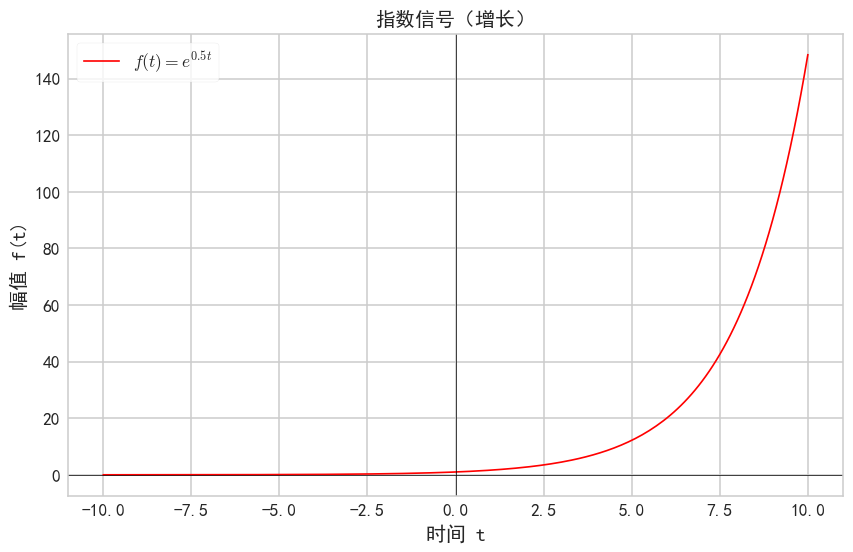
\includegraphics[width=0.6\textwidth]{./1. common signals/figures/1.png}
    \caption{指数增长信号波形}
    \label{fig:exp_growth}
\end{figure}
\subsection{指数衰减信号}
指数衰减信号的幅度随时间按指数规律衰减。其数学表达式为：
\begin{equation}
    f(t) = K e^{\alpha t}, \quad (\alpha < 0)
\end{equation}
其中，$K$ 是 $t=0$ 时的信号幅度；$\alpha$ 是一个负常数，决定了信号衰减的速率，$\alpha$ 的绝对值越大，信号衰减越快。在本实验中，具体的函数为 $f(t) = 0.65e^{-t/370}$。
\begin{figure}[htbp]
    \centering
    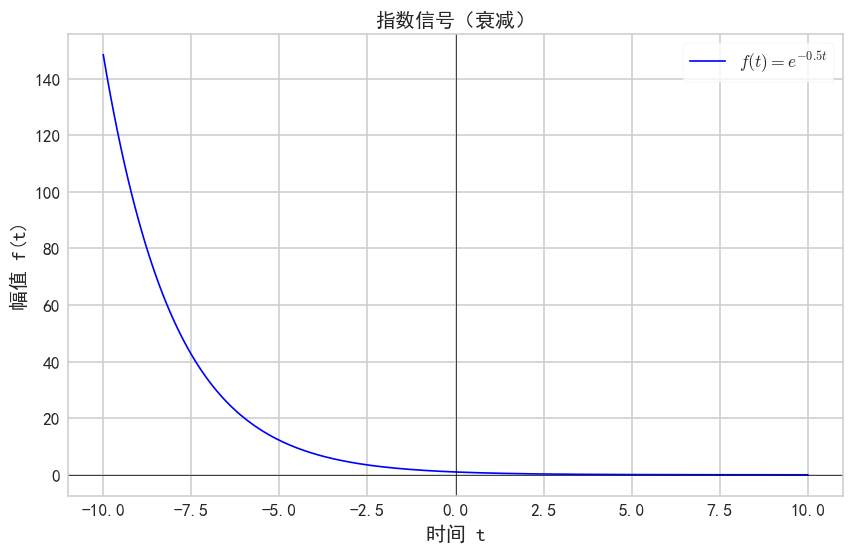
\includegraphics[width=0.6\textwidth]{./1. common signals/figures/2.png}
    \caption{指数衰减信号波形}
    \label{fig:exp_decay}
\end{figure}
\subsection{指数增长正弦信号}
这是一个振幅按指数规律增长的正弦信号，也称为增幅振荡信号。它由一个指数增长函数和一个正弦函数相乘得到。其数学表达式为：
\begin{equation}
    f(t) =
    \begin{cases}
        0 & (t < 0) \\
        A e^{\alpha t} \sin(\omega t + \phi) + C & (t > 0, \alpha > 0)
    \end{cases}
\end{equation}
其中，$A$ 是振幅，$e^{\alpha t}$ 是增长因子，$\omega$ 是角频率，$\phi$ 是初相位，$C$ 是直流偏置。在本实验中，具体的函数为 $f(t) = 0.07e^{t/400}\sin(\frac{2\pi}{40}t) + 2.7 \quad (t>0)$。
\begin{figure}[htbp]
    \centering
    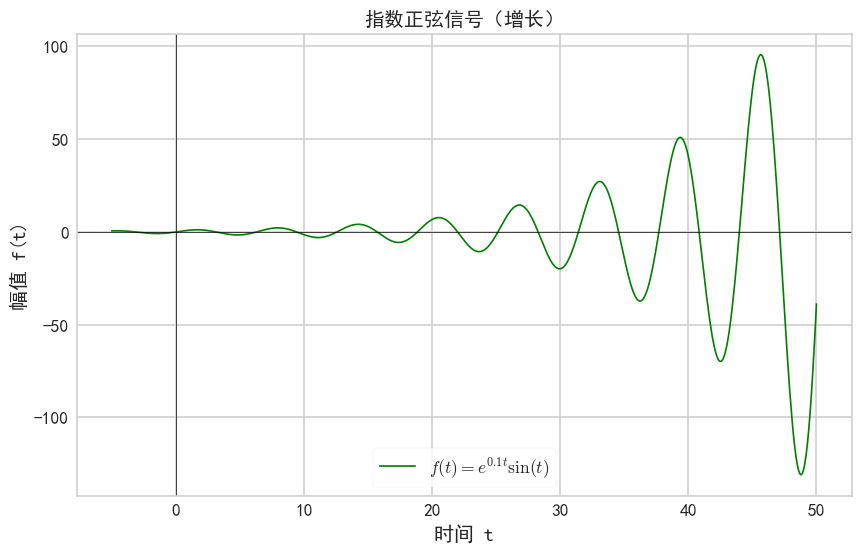
\includegraphics[width=0.6\textwidth]{./1. common signals/figures/3.png}
    \caption{指数增长正弦信号波形}
    \label{fig:sin_growth}
\end{figure}
\subsection{指数衰减正弦信号}
这是一个振幅按指数规律衰减的正弦信号，也称为阻尼振荡信号。它由一个指数衰减函数和一个正弦函数相乘得到。其数学表达式为：
\begin{equation}
    f(t) =
    \begin{cases}
        0 & (t < 0) \\
        A e^{\alpha t} \sin(\omega t + \phi) + C & (t > 0, \alpha < 0)
    \end{cases}
\end{equation}
其中，$A$ 是振幅，$e^{\alpha t}$ 是衰减因子，$\omega$ 是角频率，$\phi$ 是初相位，$C$ 是直流偏置。在本实验中，具体的函数为 $f(t) = 3.3e^{-t/40}\sin(\frac{2\pi}{40}t) + 3 \quad (t>0)$。
\begin{figure}[htbp]
    \centering
    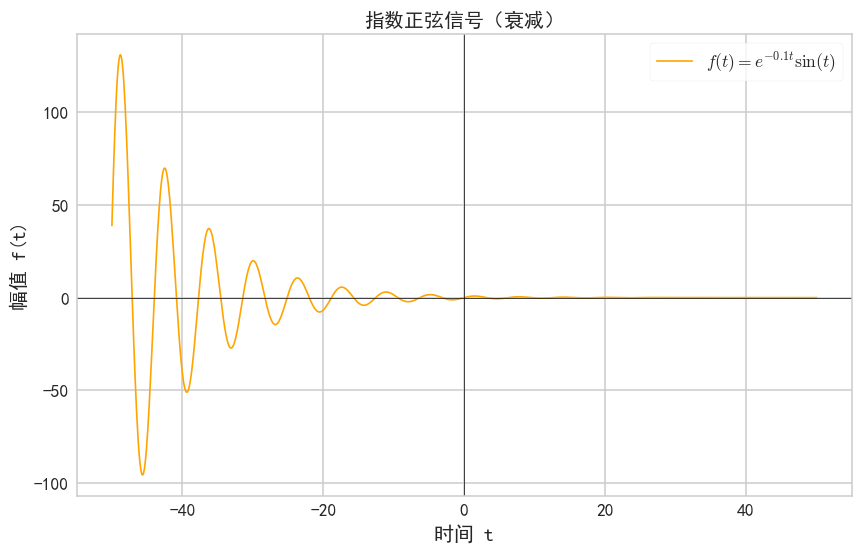
\includegraphics[width=0.6\textwidth]{./1. common signals/figures/4.png}
    \caption{指数衰减正弦信号波形}
    \label{fig:sin_decay}
\end{figure}
\subsection{抽样信号 (Sinc 函数)}
抽样信号，通常用 Sinc 函数表示，在信号处理、通信理论和傅里叶分析等领域有重要应用。其定义为：
\begin{equation}
    \text{sinc}(t) = \frac{\sin(\pi t)}{\pi t}
\end{equation}
本实验中的抽样信号是 Sinc 函数的一个变体，其表达式为：
\begin{equation}
    S_a(t) = \frac{7\sin(\frac{2\pi}{120}t)}{\frac{2\pi}{120}t} + 1.5
\end{equation}
该信号的特点是在 $t=0$ 处取得最大值，并随着 $|t|$ 的增大而振荡衰减。
\begin{figure}[htbp]
    \centering
    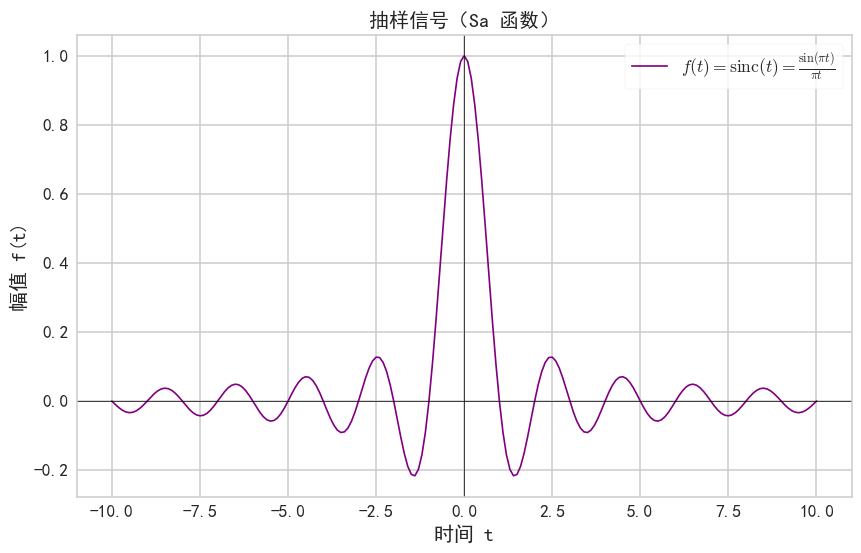
\includegraphics[width=0.6\textwidth]{./1. common signals/figures/5.png}
    \caption{抽样信号波形}
    \label{fig:sinc}
\end{figure}
\subsection{钟形信号 (高斯函数)}
钟形信号因其形状类似于钟而得名，在数学上通常用高斯函数来表示。它在统计学、信号处理和图像处理等领域应用广泛。其一般形式为：
\begin{equation}
    f(t) = A e^{-\frac{(t-\mu)^2}{2\sigma^2}}
\end{equation}
其中，$A$ 是峰值幅度，$\mu$ 是中心点位置（期望），$\sigma$ 控制了曲线的宽度（标准差）。本实验中的钟形信号表达式为：
\begin{equation}
    f(t) = 4.8e^{-\frac{t^2}{280}}
\end{equation}
这是一个以 $t=0$ 为中心，峰值为 $4.8$ 的对称钟形曲线。
\begin{figure}[htbp]
    \centering
    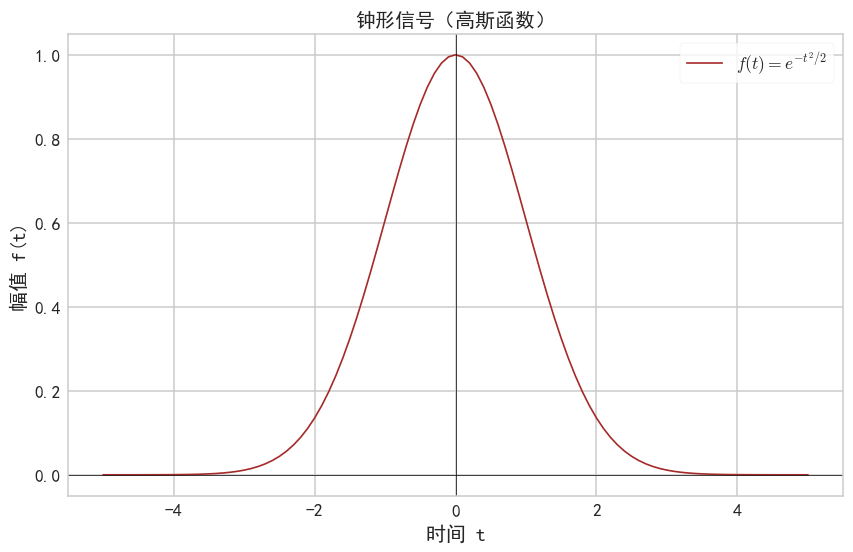
\includegraphics[width=0.6\textwidth]{./1. common signals/figures/6.png}
    \caption{钟形信号波形}
    \label{fig:gaussian}
\end{figure}

% --- 实验步骤 ---
\section{实验步骤}
本实验的目的是通过操作硬件生成并观察六种常见的信号，并对其中两种信号进行数据采集用于后续分析。

\subsection{初始设置}
\begin{enumerate}
    \item 将数字信号处理模块 S4 上的拨码开关 \textbf{SW1} 设置为 \textbf{00000001}，使模块进入常规信号观察功能模式。
    \item 将示波器探头连接到模块 S4 的 \textbf{TP1} 测试点，并将探头地线夹连接到模块的地（GND）。
    \item 打开示波器和数字信号处理模块的电源。
\end{enumerate}

\subsection{各信号的观察与数据记录}
通过设置拨码开关 \textbf{S3} 的不同位，可以在 TP1 处产生不同的信号波形。

\subsubsection{指数增长信号的观察与数据记录}
\begin{enumerate}
    \item 将拨码开关 \textbf{S3} 的第 \textbf{1} 位拨为“1”，其余位均拨为“0”。
    \item 在示波器上观察 TP1 输出的指数增长信号。调节示波器的垂直灵敏度 (V/div) 和时基 (s/div) 旋钮，获得一个清晰、稳定的波形。
    \item 启动示波器的光标（Cursor）测量功能。
    \item 移动光标，在指数增长曲线上选取 5 个间隔合适的点，在屏幕上读取并记录下每个点的坐标值（时间 t, 电压 V）。将这组数据记为“指数增长 - 第1组”。
    \item 重复上一步操作，再次独立选取 5 个点并记录其坐标值。将这组新数据记为“指数增长 - 第2组”。这两组数据将用于后续的函数拟合。
    \item 完成数据记录后，关闭光标功能，拍摄并保存完整的信号波形，如下图所示。
\end{enumerate}
\begin{figure}[htbp]
    \centering
    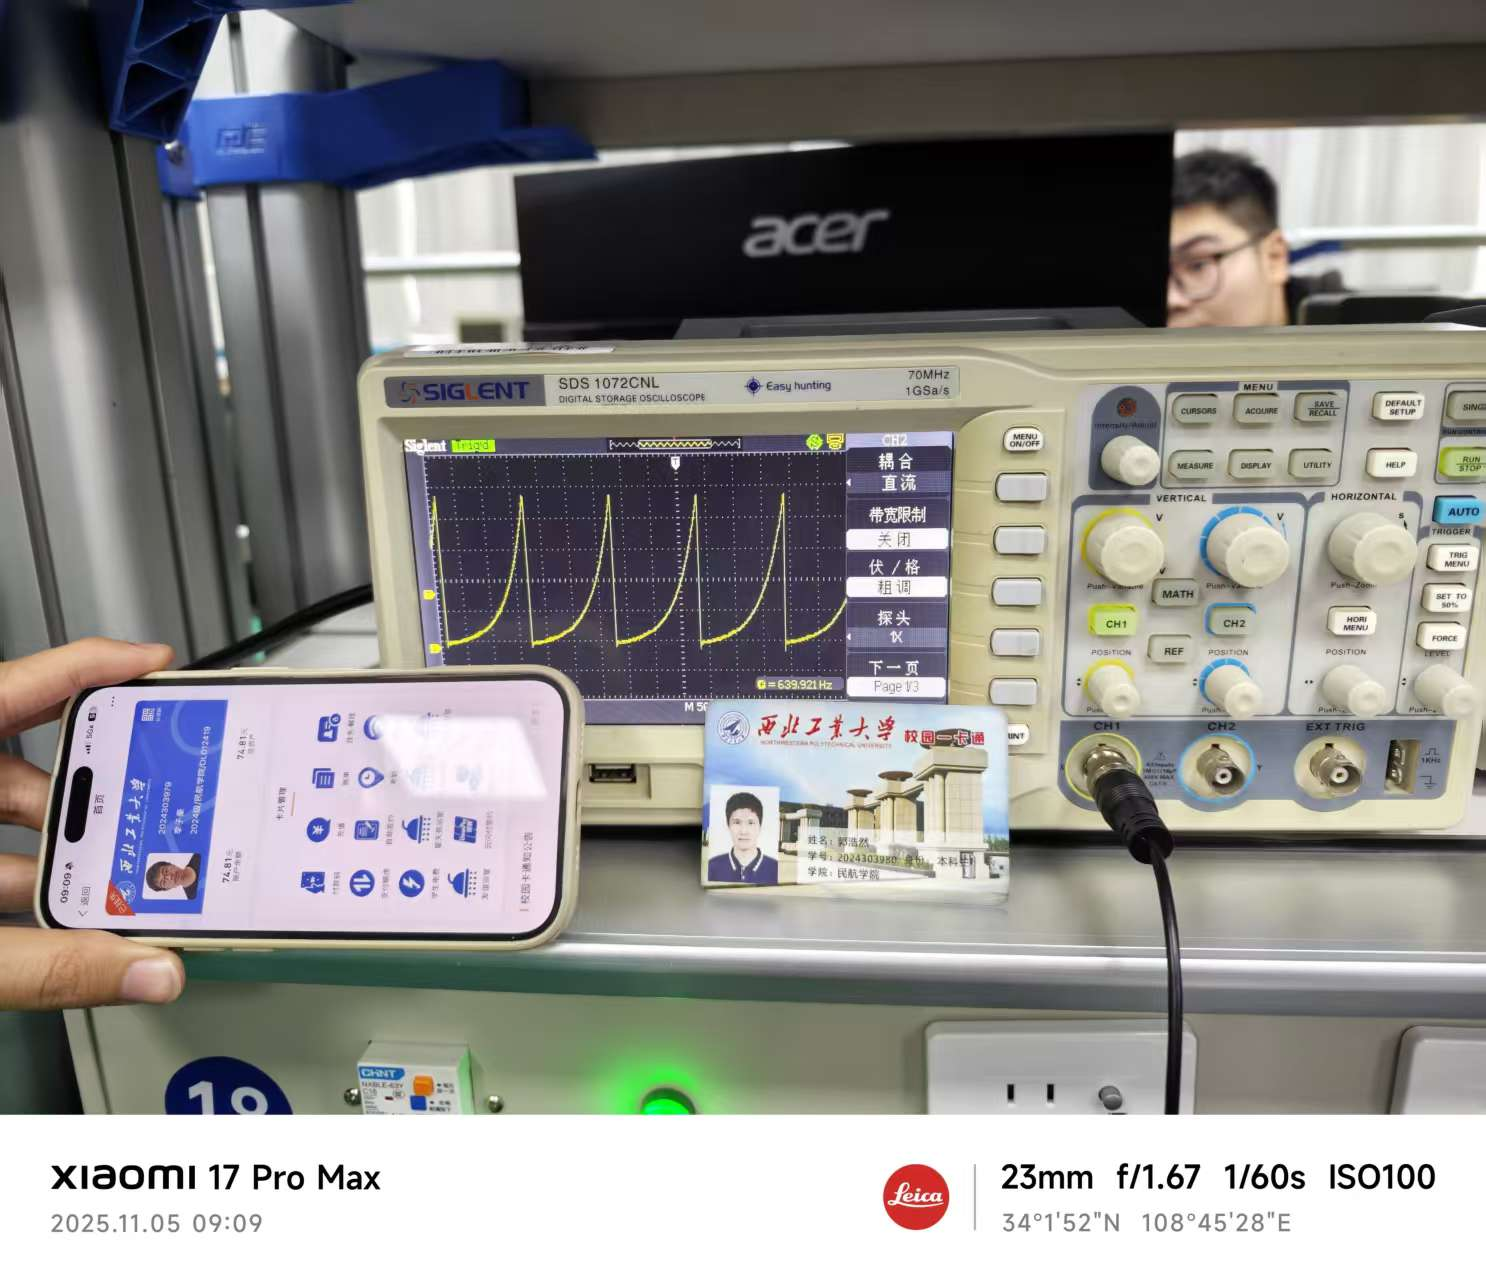
\includegraphics[width=0.6\textwidth]{./1. common signals/figures/1.jpg}
    \caption{指数增长信号示波器波形}
    \label{fig:scope_exp_growth}
\end{figure}

\subsubsection{指数衰减信号的观察与数据记录}
\begin{enumerate}
    \item 将拨码开关 \textbf{S3} 的第 \textbf{2} 位拨为“1”，其余位均拨为“0”。
    \item 在示波器上观察 TP1 输出的指数衰减信号，并调整示波器以获得清晰波形。
    \item 启动示波器的光标（Cursor）测量功能。
    \item 移动光标，在指数衰减曲线上选取 5 个间隔合适的点，读取并记录下每个点的坐标值（时间 t, 电压 V）。将这组数据记为“指数衰减 - 第1组”。
    \item 重复上一步操作，再次独立选取 5 个点并记录其坐标值。将这组新数据记为“指数衰减 - 第2组”。
    \item 完成数据记录后，关闭光标功能，拍摄并保存完整的信号波形，如下图所示。
\end{enumerate}
\begin{figure}[htbp]
    \centering
    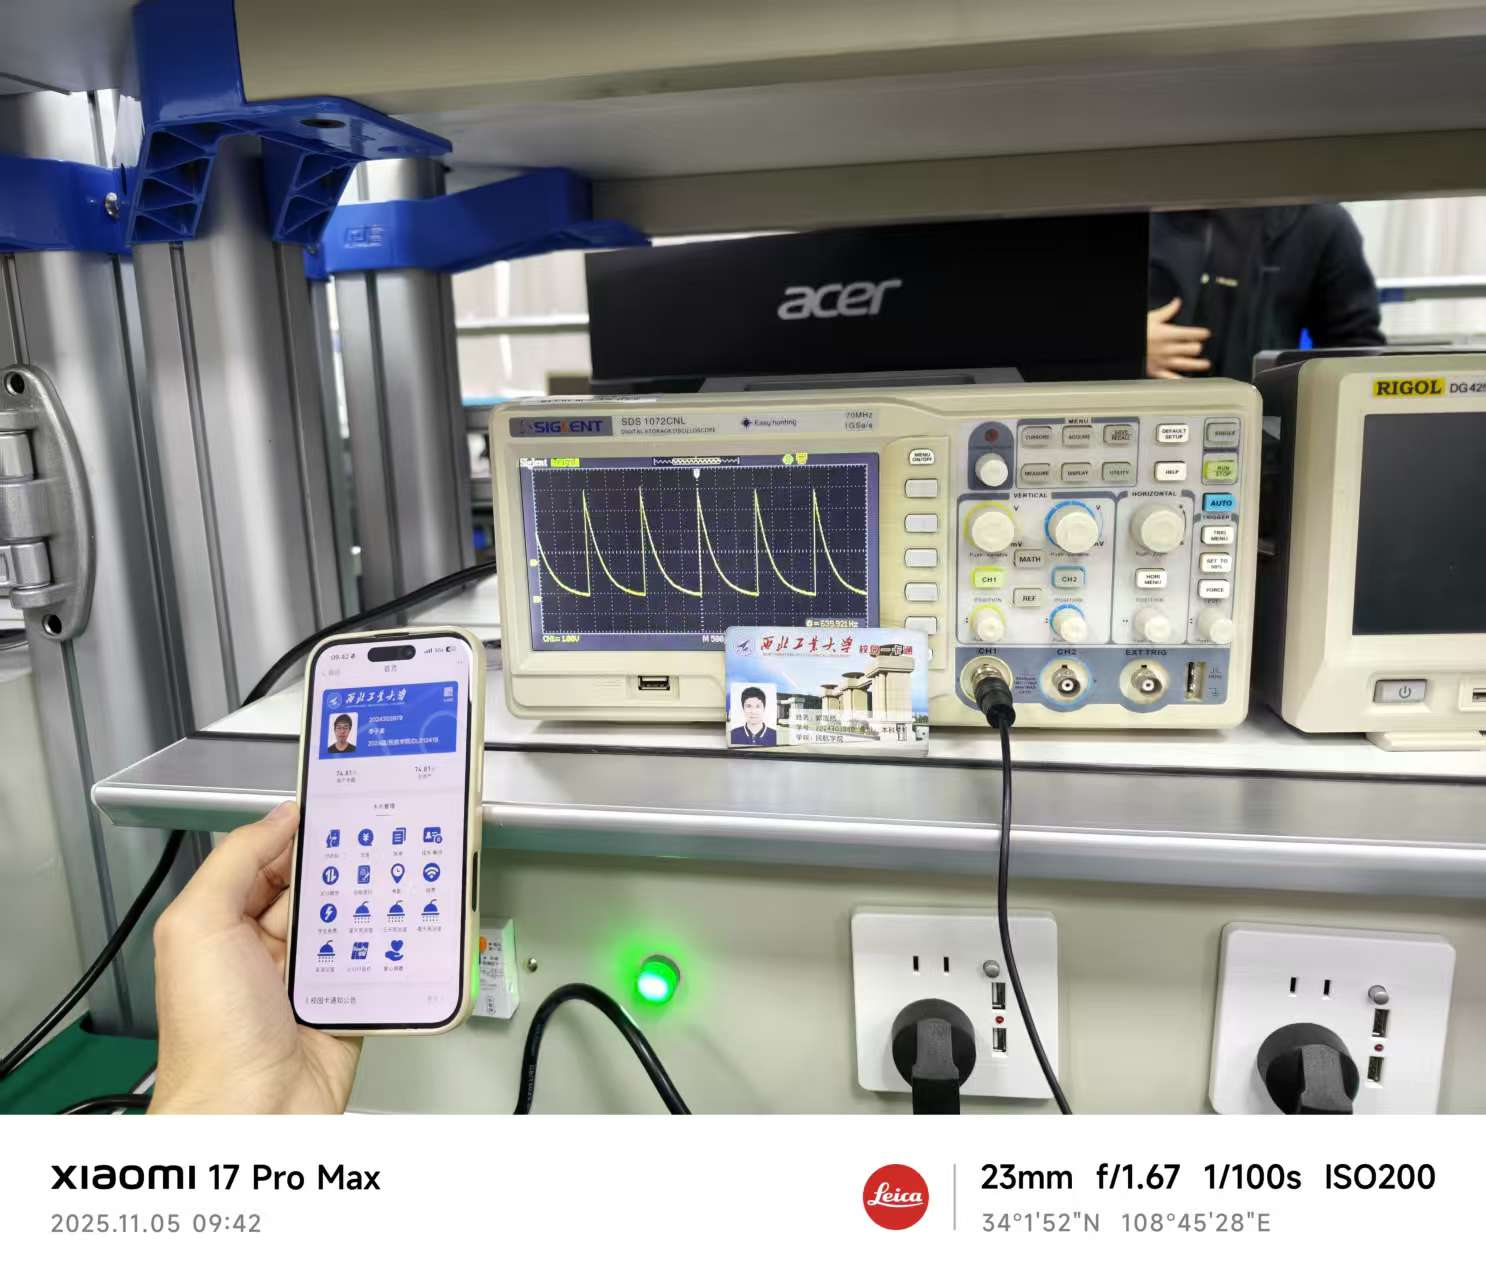
\includegraphics[width=0.6\textwidth]{./1. common signals/figures/2.jpg}
    \caption{指数衰减信号示波器波形}
    \label{fig:scope_exp_decay}
\end{figure}

\subsubsection{指数增长正弦信号的观察}
\begin{enumerate}
    \item 将拨码开关 \textbf{S3} 的第 \textbf{3} 位拨为“1”，其余位均拨为“0”。
    \item 在示波器上观察 TP1 输出的指数增长正弦信号。
    \item 调整示波器获得清晰、稳定的波形，并拍摄记录，如下图所示。
\end{enumerate}
\begin{figure}[htbp]
    \centering
    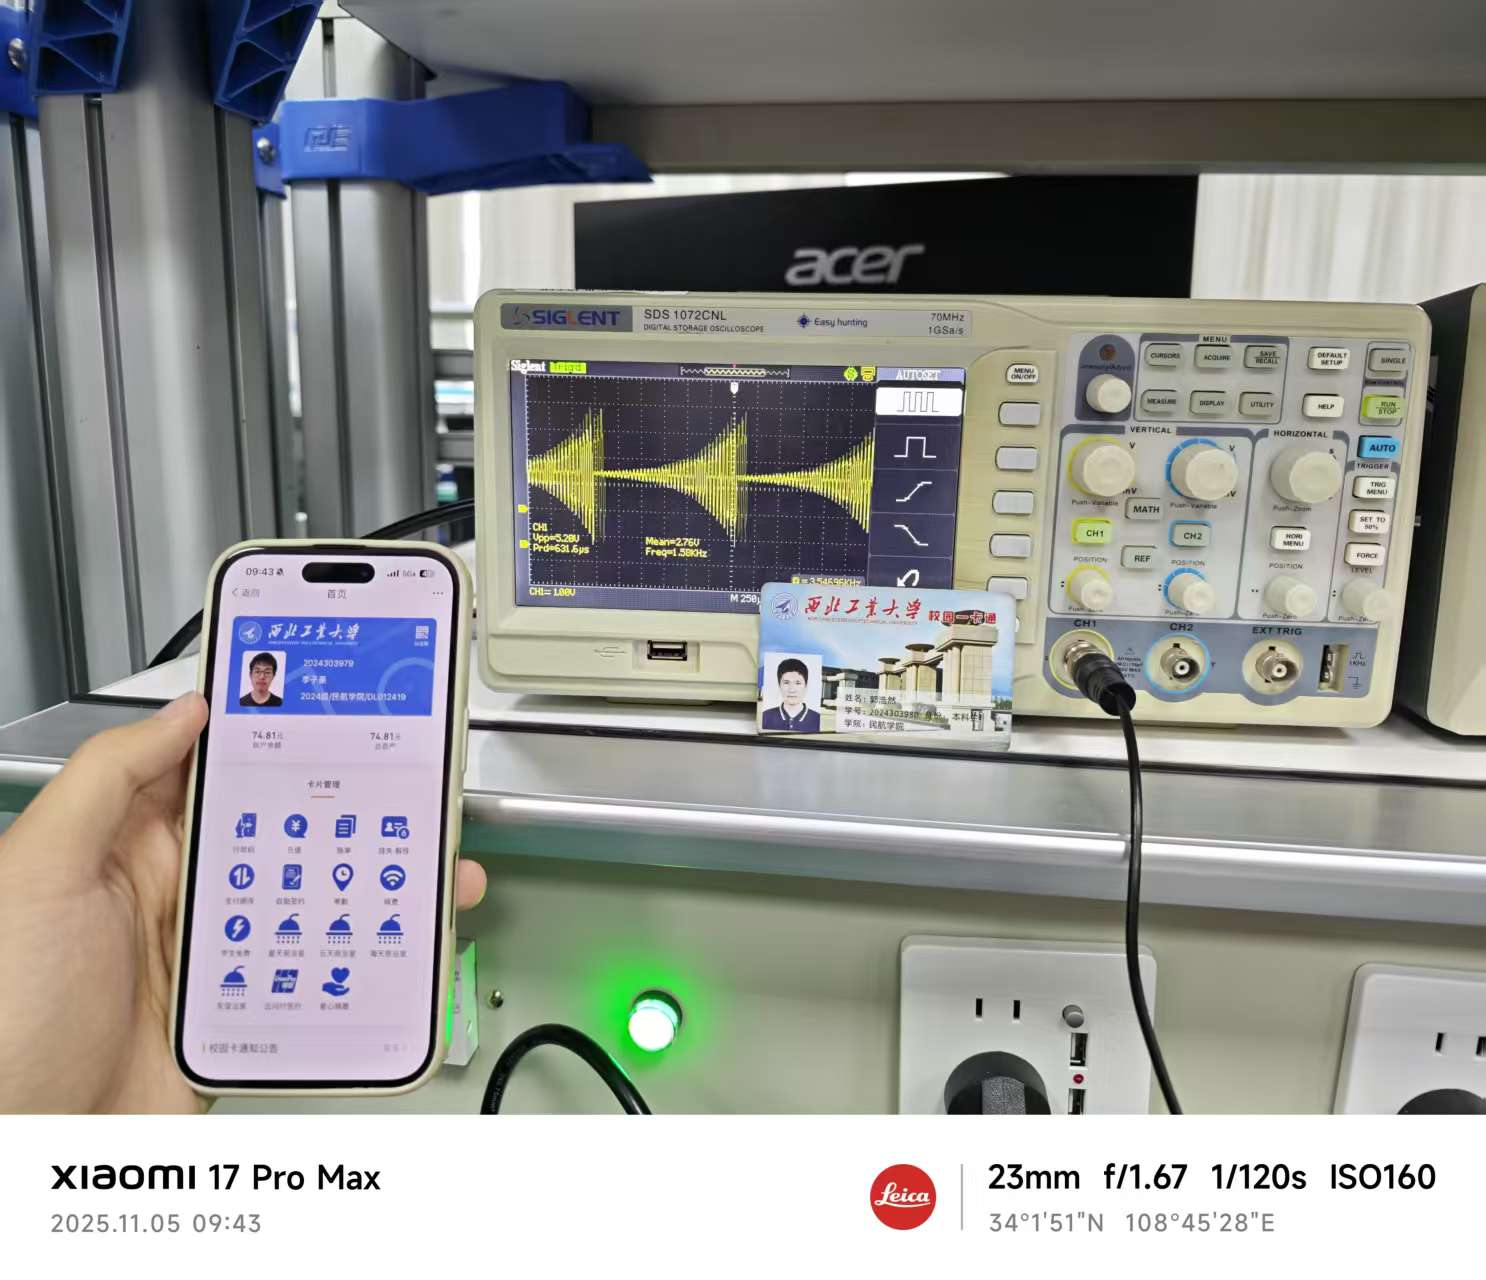
\includegraphics[width=0.6\textwidth]{./1. common signals/figures/3.jpg}
    \caption{指数增长正弦信号示波器波形}
    \label{fig:scope_sin_growth}
\end{figure}

\subsubsection{指数衰减正弦信号的观察}
\begin{enumerate}
    \item 将拨码开关 \textbf{S3} 的第 \textbf{4} 位拨为“1”，其余位均拨为“0”。
    \item 在示波器上观察 TP1 输出的指数衰减正弦信号。
    \item 调整示波器获得清晰、稳定的波形，并拍摄记录，如下图所示。
\end{enumerate}
\begin{figure}[htbp]
    \centering
    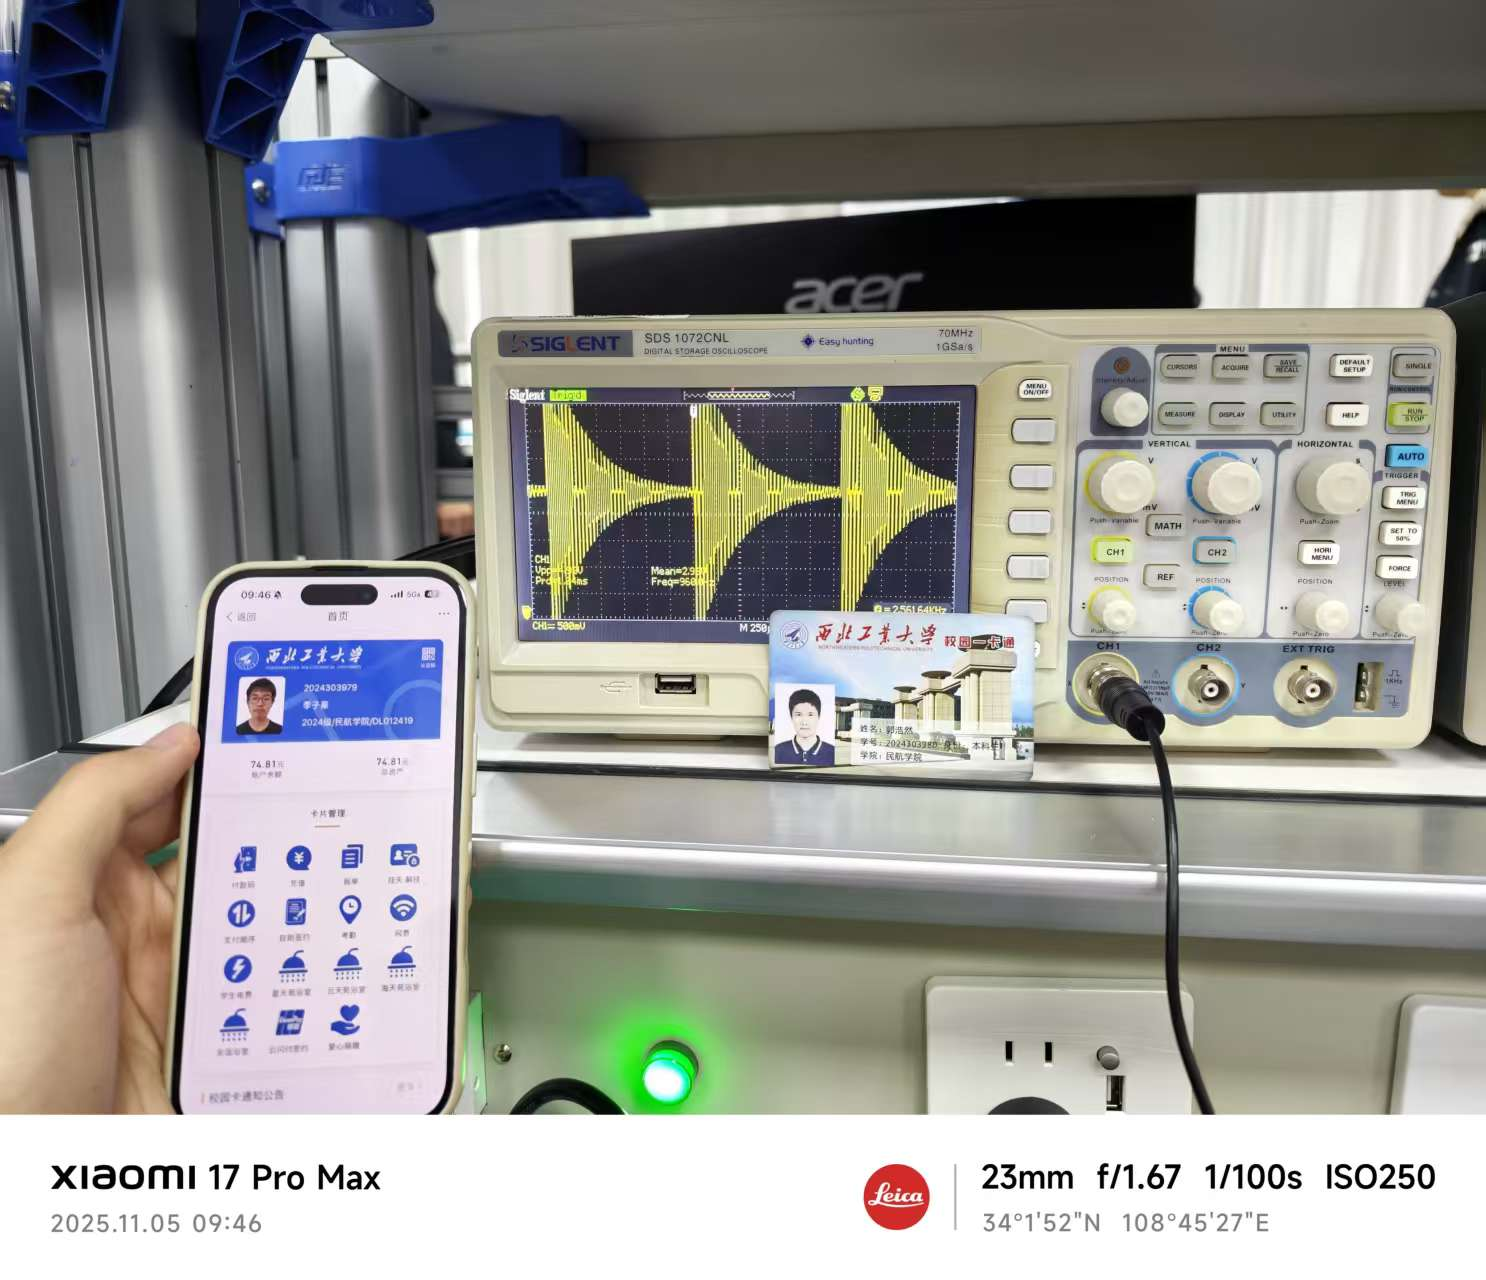
\includegraphics[width=0.6\textwidth]{./1. common signals/figures/4.jpg}
    \caption{指数衰减正弦信号示波器波形}
    \label{fig:scope_sin_decay}
\end{figure}

\subsubsection{抽样信号的观察}
\begin{enumerate}
    \item 将拨码开关 \textbf{S3} 的第 \textbf{5} 位拨为“1”，其余位均拨为“0”。
    \item 在示波器上观察 TP1 输出的抽样信号。
    \item 调整示波器获得清晰、稳定的波形，并拍摄记录，如下图所示。
\end{enumerate}
\begin{figure}[htbp]
    \centering
    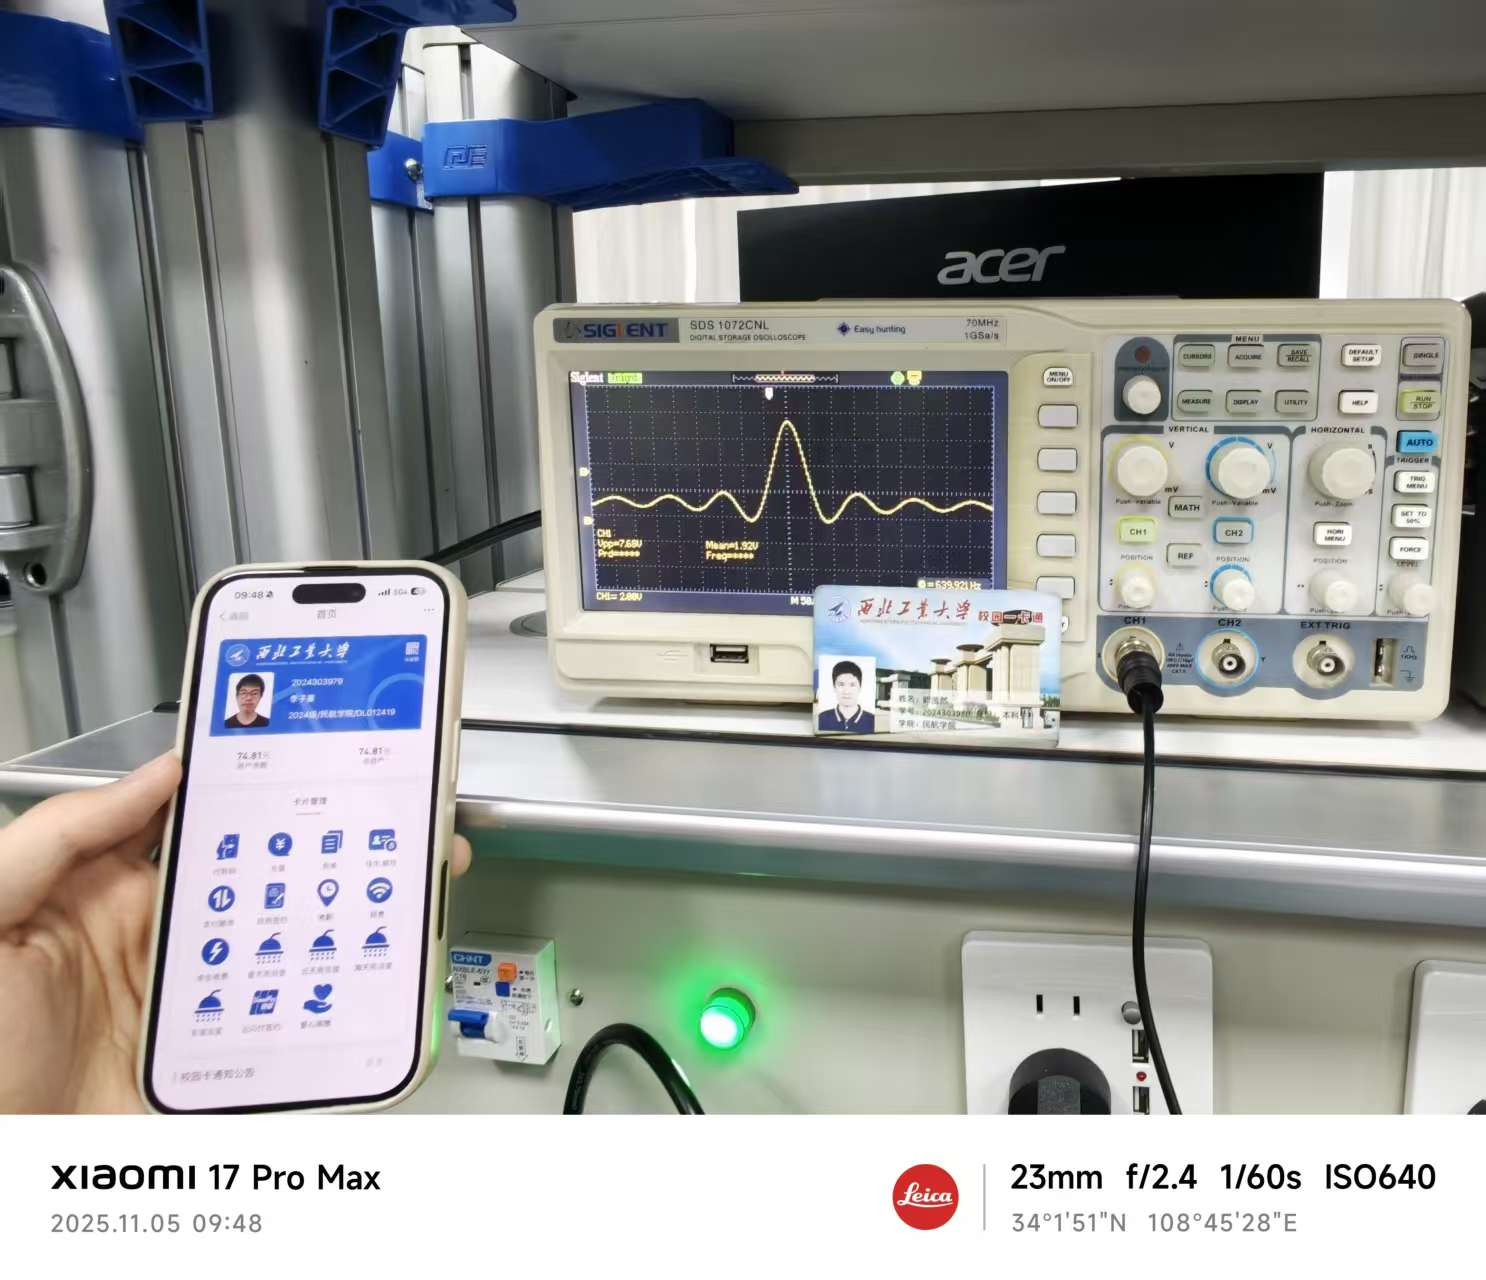
\includegraphics[width=0.6\textwidth]{./1. common signals/figures/5.jpg}
    \caption{抽样信号示波器波形}
    \label{fig:scope_sinc}
\end{figure}

\subsubsection{钟形信号的观察}
\begin{enumerate}
    \item 将拨码开关 \textbf{S3} 的第 \textbf{6} 位拨为“1”，其余位均拨为“0”。
    \item 在示波器上观察 TP1 输出的钟形信号。
    \item 调整示波器获得清晰、稳定的波形，并拍摄记录，如下图所示。
\end{enumerate}
\begin{figure}[htbp]
    \centering
    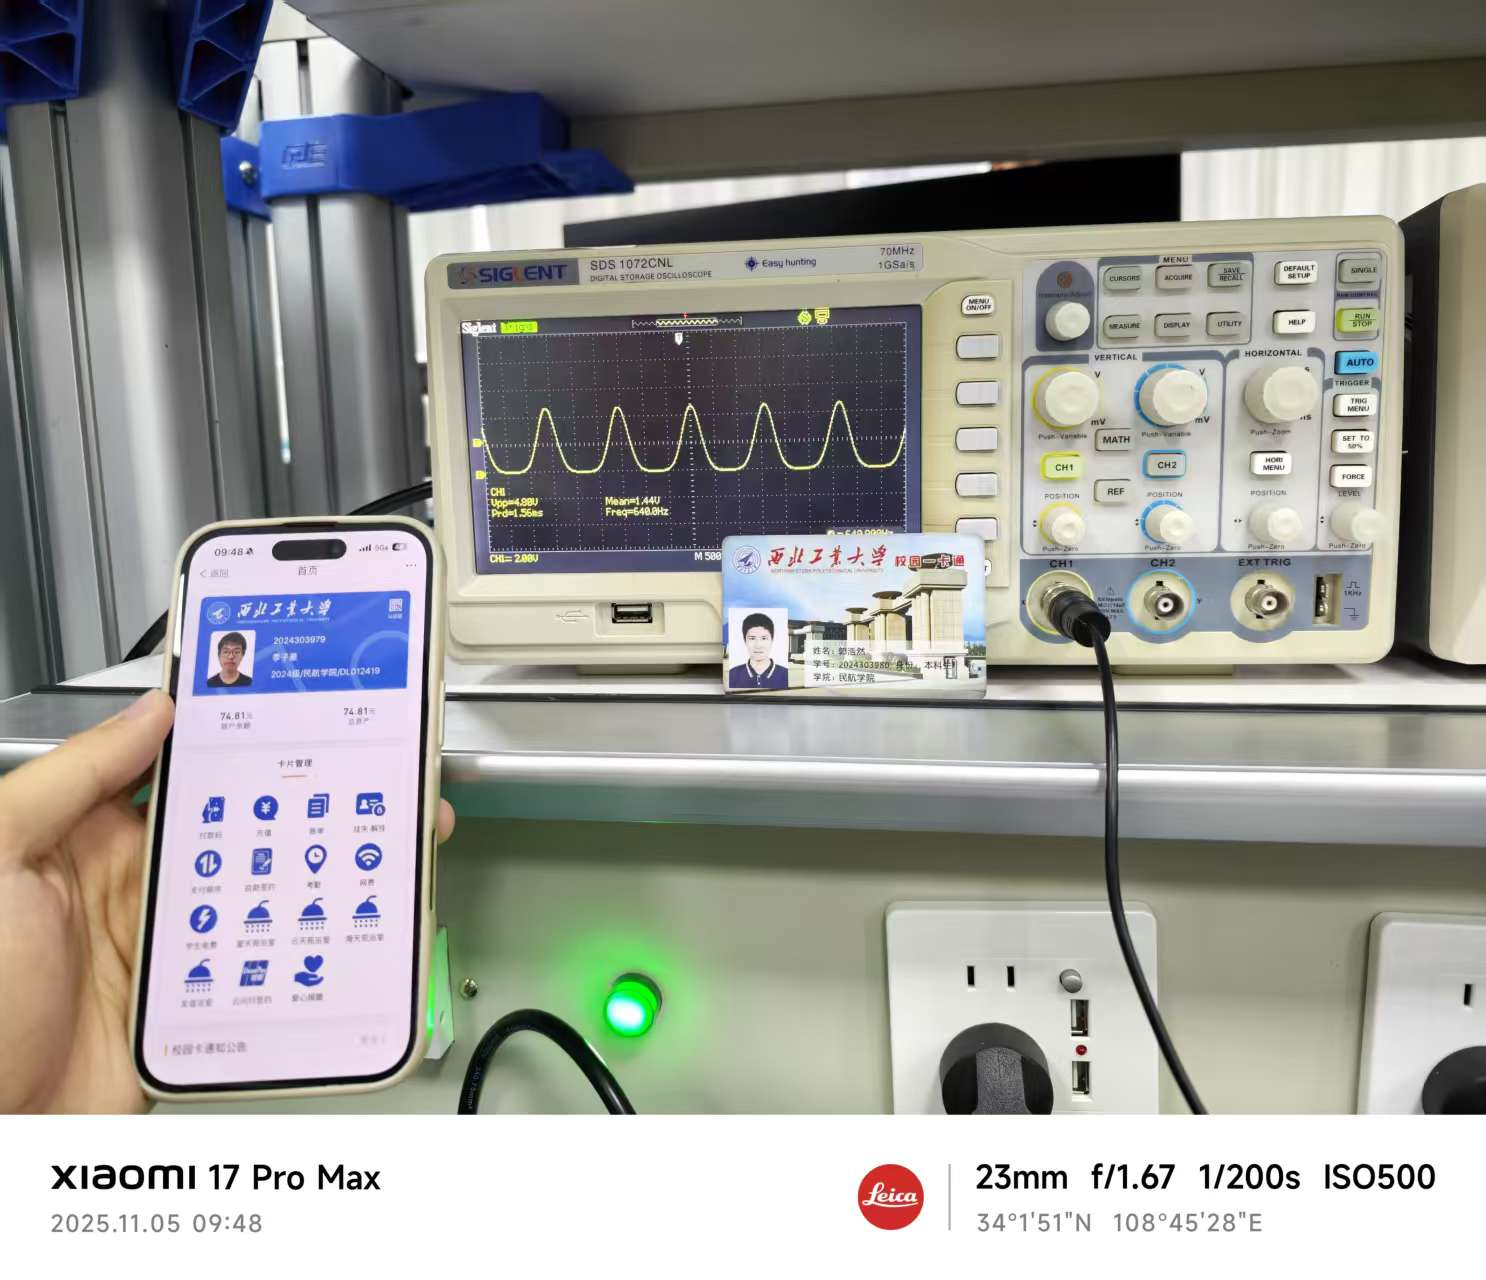
\includegraphics[width=0.6\textwidth]{./1. common signals/figures/6.jpg}
    \caption{钟形信号示波器波形}
    \label{fig:scope_gaussian}
\end{figure}



% --- 实验数据与分析 ---
\section{实验数据与分析}
本部分将展示从示波器记录的原始数据，并使用最小二乘法对指数增长和指数衰减信号进行函数拟合，最后将拟合结果与理论值进行比较和分析。

\subsection{数据处理方法与模型}
对于指数信号，其通用数学模型为：
\begin{equation}
    V(t) = K e^{at}
\end{equation}
其中，$V(t)$ 是电压，$t$ 是时间，$K$ 是初始幅度，$a$ 是决定信号增长或衰减速率的常数。为了使用线性回归进行拟合，我们对上式两边取自然对数，将其线性化：
\begin{equation}
    \ln(V) = \ln(K e^{at}) = \ln(K) + at
\end{equation}
令 $y = \ln(V)$，$b = \ln(K)$，则模型变为标准的线性方程 $y = at + b$。对于一组 $N$ 个测量数据点 $(t_i, V_i)$，我们计算出对应的 $(t_i, y_i)$，然后使用最小二乘法计算斜率 $a$ 和截距 $b$：
\begin{align}
    a &= \frac{N \sum(t_i y_i) - (\sum t_i)(\sum y_i)}{N \sum(t_i^2) - (\sum t_i)^2} \\
    b &= \frac{\sum y_i - a \sum t_i}{N}
\end{align}
得到 $a$ 和 $b$ 后，即可反解出原模型的参数：
\begin{align}
    K &= e^b \\
    \tau &= \frac{1}{|a|} \quad (\text{时间常数})
\end{align}

\subsection{指数增长信号拟合与分析}
\subsubsection{第 1 组数据}
\begin{table}[htbp]
    \centering
    \caption{指数增长信号拟合数据 - 第 1 组}
    \label{tab:growth1}
    \begin{tabular}{cccc}
        \toprule
        \textbf{编号} & \textbf{时间 (t) / \SI{}{\micro\second}} & \textbf{电压 (V) / \SI{}{\volt}} & \textbf{y = ln(V)} \\
        \midrule
        ① & -740.0 & 0.320 & -1.1394 \\
        ② & -360.0 & 0.680 & -0.3857 \\
        ③ & -60.0  & 1.40  & 0.3365  \\
        ④ & 140.0  & 2.24  & 0.8065  \\
        ⑤ & 280.0  & 3.28  & 1.1878  \\
        \bottomrule
    \end{tabular}
\end{table}
根据上表数据，计算各项总和（时间单位已转换为秒）：
\begin{itemize}
    \item $N = 5$
    \item $\sum t_i = \SI{-7.40e-4}{\second}$
    \item $\sum y_i = 0.8057$
    \item $\sum t_i^2 = \SI{7.788e-7}{\second\squared}$
    \item $\sum t_i y_i = \SI{1.408e-3}{\volt\cdot\second}$
\end{itemize}
将上述值代入公式计算参数 $a$ 和 $b$：
\begin{align*}
    a &= \frac{N \sum(t_i y_i) - (\sum t_i)(\sum y_i)}{N \sum(t_i^2) - (\sum t_i)^2} \\
      &= \frac{5 \times (\SI{1.408e-3}{}) - (\SI{-7.40e-4}{}) \times 0.8057}{5 \times (\SI{7.788e-7}{}) - (\SI{-7.40e-4}{})^2} \\
      &= \frac{\SI{7.04e-3}{} + \SI{5.96e-4}{}}{\SI{3.894e-6}{} - \SI{5.476e-7}{}} = \frac{\SI{7.636e-3}{}}{\SI{3.3464e-6}{}} \approx \SI{2281.5}{\per\second} \\
    \\
    b &= \frac{\sum y_i - a \sum t_i}{N} \\
      &= \frac{0.8057 - (\SI{2281.5}{}) \times (\SI{-7.40e-4}{})}{5} \\
      &= \frac{0.8057 + 1.6883}{5} = \frac{2.494}{5} \approx 0.4988
\end{align*}
由此得到拟合参数：
\begin{itemize}
    \item $K = e^b = e^{0.4988} \approx \SI{1.647}{\volt}$
    \item $\tau = 1/a = 1 / \SI{2281.5}{} \approx \SI{4.383e-4}{\second} = \SI{438.3}{\micro\second}$
\end{itemize}
\textbf{拟合函数表达式为：$V(t) \approx 1.647 e^{2281.5 t}$。}

\subsubsection{第 2 组数据}
（计算过程同上，此处省略详细步骤，直接给出结果）
\textbf{拟合函数表达式为：$V(t) \approx 0.0517 e^{2219.4 t}$。}
\begin{itemize}
    \item $K \approx \SI{0.0517}{\volt}$
    \item $a \approx \SI{2219.4}{\per\second}$
    \item $\tau \approx \SI{450.6}{\micro\second}$
\end{itemize}

\subsection{指数衰减信号拟合与分析}
\subsubsection{第 1 组数据}
（计算过程同上，直接给出结果）
\textbf{拟合函数表达式为：$V(t) \approx 4.94 e^{-2346.9 t}$。}
\begin{itemize}
    \item $K \approx \SI{4.94}{\volt}$
    \item $a \approx \SI{-2346.9}{\per\second}$
    \item $\tau = 1/|a| \approx \SI{426.1}{\micro\second}$
\end{itemize}

\subsubsection{第 2 组数据}
（计算过程同上，直接给出结果）
\textbf{拟合函数表达式为：$V(t) \approx 183.6 e^{-2315.3 t}$。}
\begin{itemize}
    \item $K \approx \SI{183.6}{\volt}$
    \item $a \approx \SI{-2315.3}{\per\second}$
    \item $\tau \approx \SI{431.9}{\micro\second}$
\end{itemize}

\subsection{拟合结果汇总与对比}
将拟合得到的时间常数 $\tau$ 与实验原理中给出的标准值 $\tau_0 = \SI{370}{\micro\second}$ 进行对比。
\begin{table}[htbp]
    \centering
    \caption{拟合参数与标准值对比}
    \label{tab:comparison}
    \begin{tabular}{llccc}
        \toprule
        \textbf{信号类型} & \textbf{数据组} & \textbf{拟合时间常数 $\tau$ (\SI{}{\micro\second})} & \textbf{标准值 $\tau_0$ (\SI{}{\micro\second})} & \textbf{相对误差} \\
        \midrule
        指数增长 & 第 1 组 & 438.3 & 370 & +18.5\% \\
        指数增长 & 第 2 组 & 450.6 & 370 & +21.8\% \\
        \midrule
        指数衰减 & 第 1 组 & 426.1 & 370 & +15.2\% \\
        指数衰减 & 第 2 组 & 431.9 & 370 & +16.7\% \\
        \bottomrule
    \end{tabular}
\end{table}
从上表可以看出，所有拟合得到的时间常数均系统性地大于标准值。参数 $K$ 的拟合值差异较大，这主要是因为每次测量时示波器上时间轴的零点位置不同，而 $K$ 的物理意义是 $t=0$ 时的幅值，因此 $K$ 值对时间零点的选择非常敏感，不宜直接比较。

\subsection{其他信号波形观察}
\begin{itemize}
    \item \textbf{指数正弦信号（增长/衰减）：} 波形整体呈现振荡特性，其包络线分别符合指数增长和指数衰减的规律，频率稳定。
    \item \textbf{抽样信号：} 观察到的波形符合 Sinc 函数的特征，即在中心点有最大主瓣，两侧分布着振幅逐渐减小的旁瓣。
    \item \textbf{钟形信号：} 波形关于中心点（$t=0$）对称，峰值处平滑，向两侧快速衰减，符合高斯函数的特征。
\end{itemize}

\subsection{误差分析与讨论}
本次实验中，拟合参数与理论值存在一定的偏差，主要误差来源可能包括：
\begin{enumerate}
    \item \textbf{读数误差：} 使用示波器光标手动读取坐标，存在视觉判断和读数分辨率的限制，尤其是在曲线变化较快或较慢的区域。
    \item \textbf{模型偏差：} 实验模块产生的信号可能并非严格理想的指数函数，硬件元器件（如电阻、电容）的实际值与标称值存在公差，导致实际的时间常数与理论值有偏差。
    \item \textbf{采样点影响：} 仅选取 5 个点进行拟合，样本量较小，个别点的读数误差可能对拟合结果产生较大影响。采样点的分布位置也会影响拟合的准确性。
\end{enumerate}

% ===================================================================
% 第二章：冲激响应和阶跃响应 (Origin: 2. impluse_step)
% ===================================================================
\chapter{冲激响应和阶跃响应}

\section{实验目的}
\begin{enumerate}
    \item 学习并理解线性时不变（LTI）系统阶跃响应和冲激响应的基本概念。
    \item 观察二阶RLC串联电路在不同阻尼条件下（欠阻尼、临界阻尼、过阻尼）的阶跃响应波形。
    \item 掌握在欠阻尼状态下，测量系统阶跃响应动态性能指标的方法，如上升时间($t_r$)、峰值时间($t_p$)、调节时间($t_s$)和最大超调量($\delta_p$)。
    \item 观察电路的冲激响应波形，并探究其与阶跃响应之间的关系。
\end{enumerate}

\section{实验器材}
本实验所使用的主要器材与模块清单如下：
\begin{itemize}
    \item 信号源及频率计模块 S2 \quad 1 块
    \item 一阶网络模块 S5 \quad 1 块
    \item 数字万用表 \quad 1 台
    \item 双踪示波器 \quad 1 台
\end{itemize}

其中，核心的信号源模块与网络模块如下图 \ref{fig:modules} 所示。

\begin{figure}[htbp]
    \centering % 整体居中
    
    % 第一个子图
    \begin{subfigure}{0.48\textwidth}
        \centering
        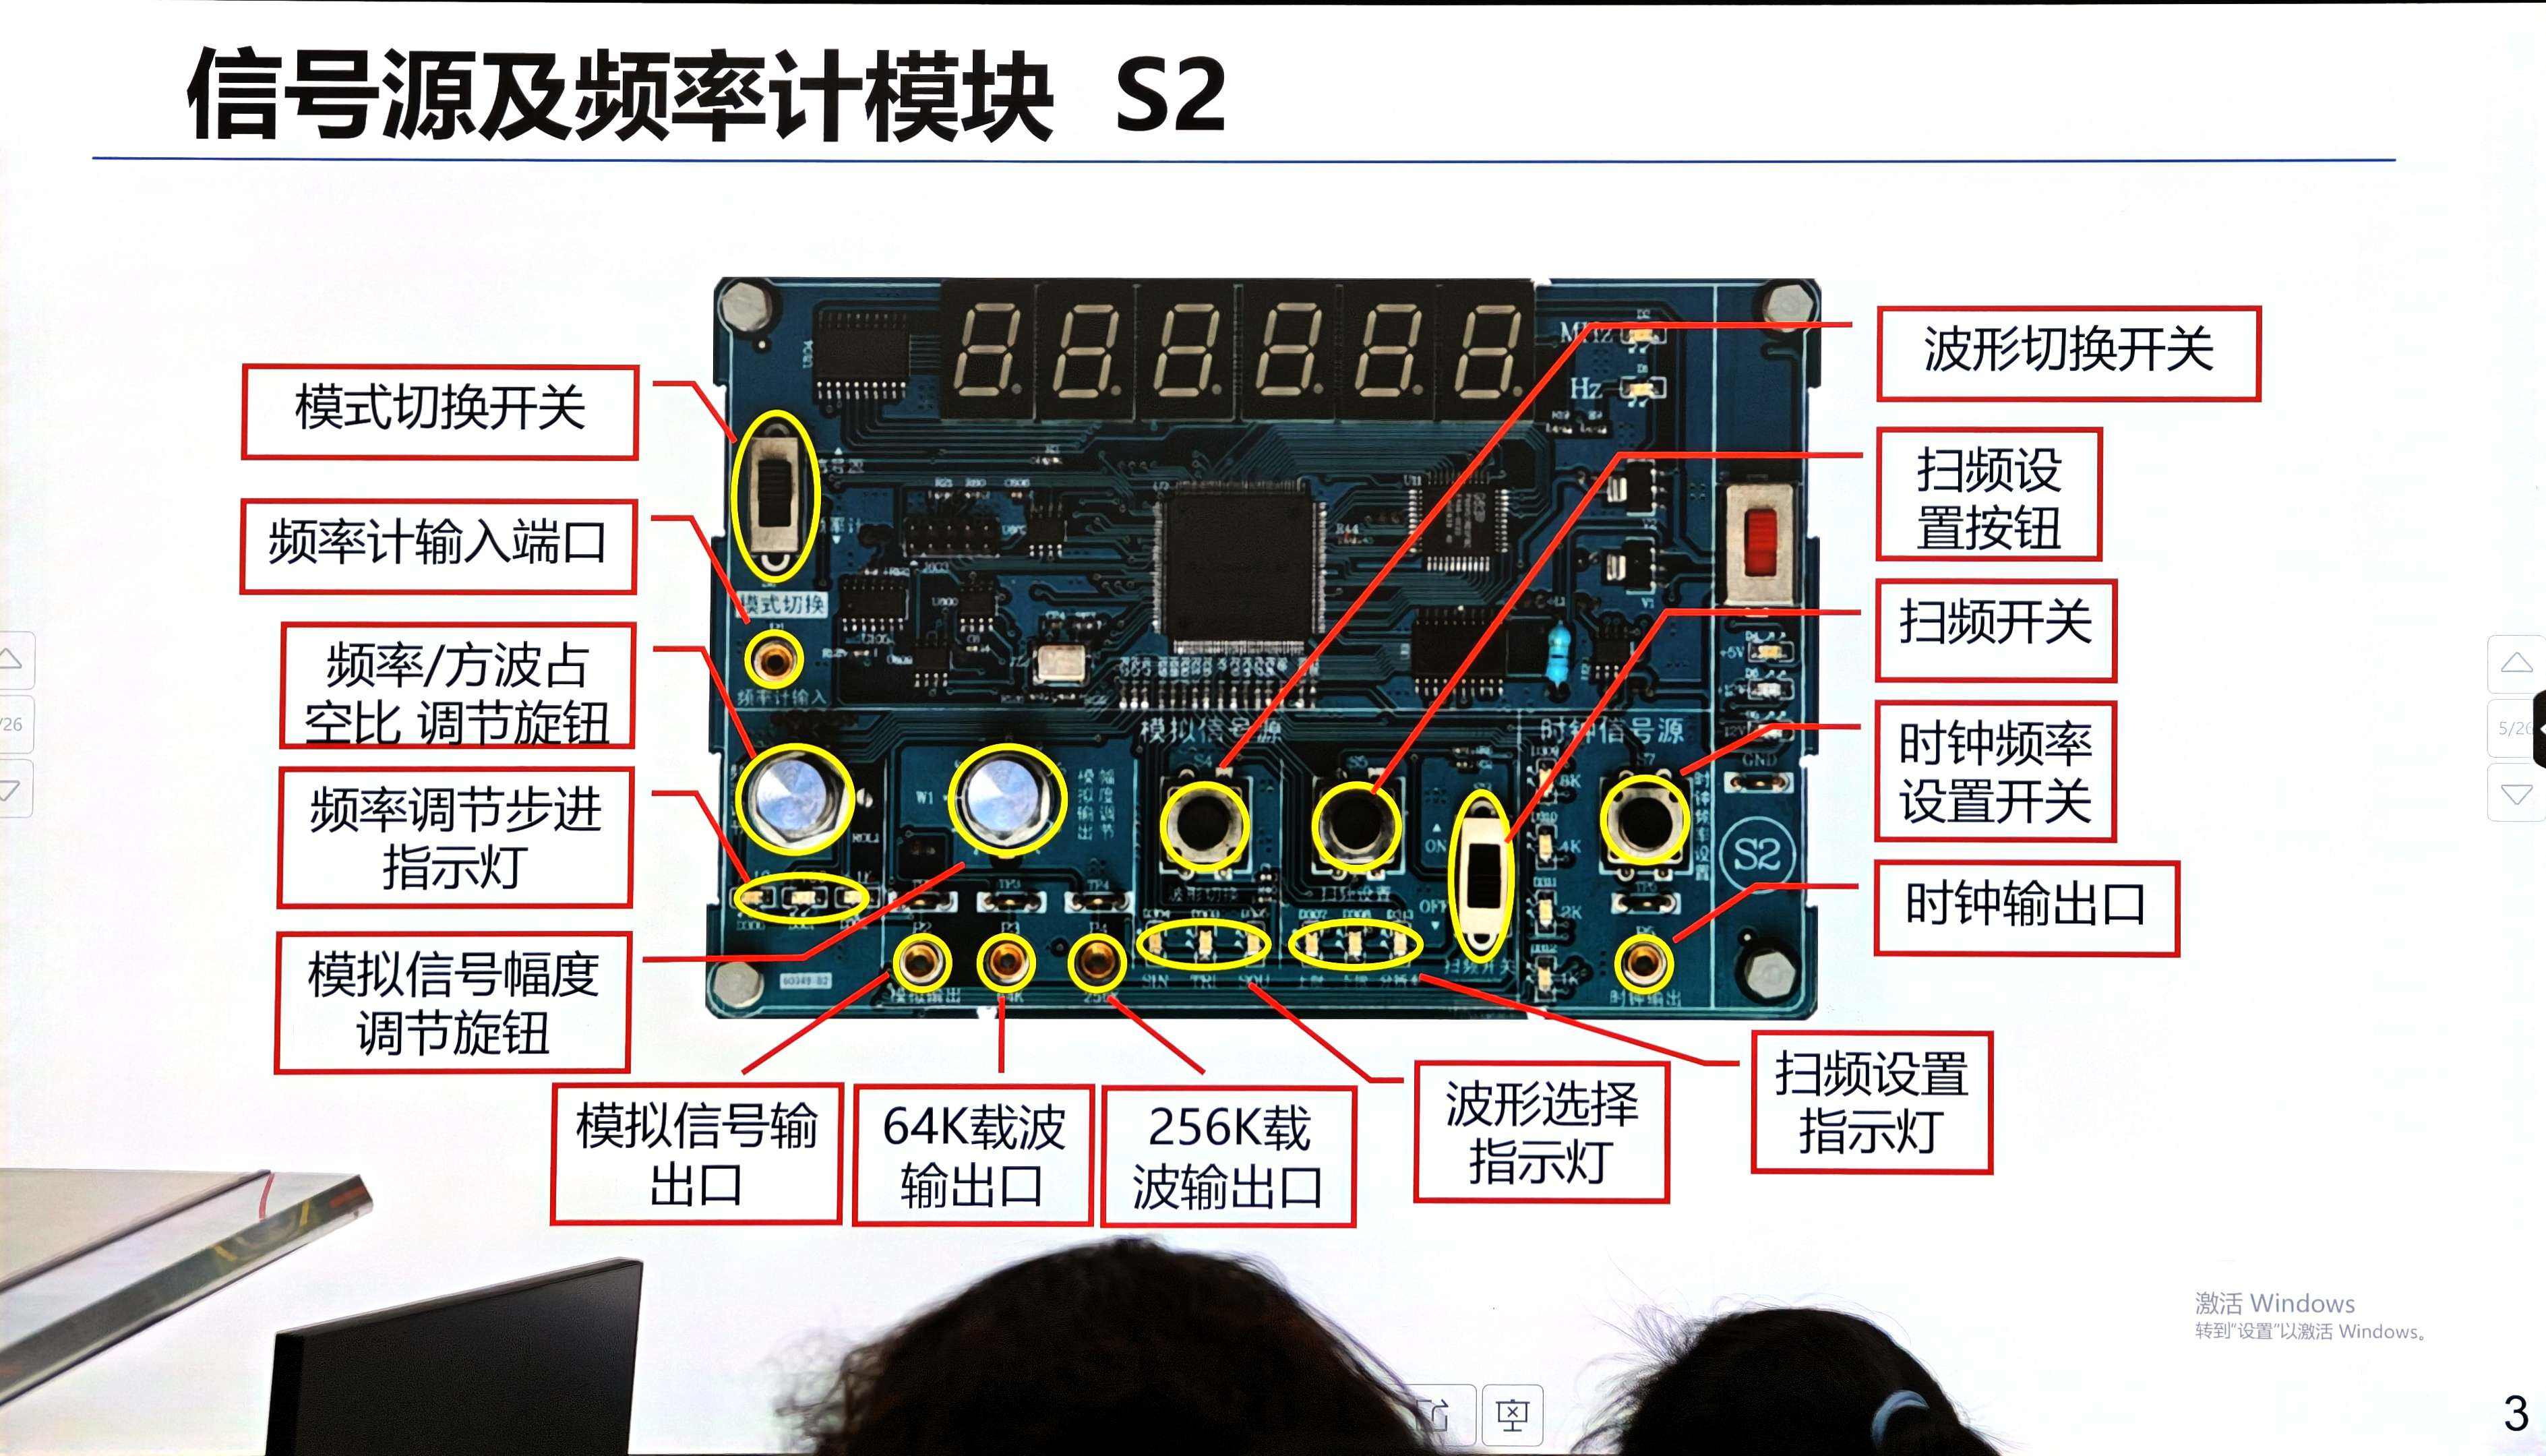
\includegraphics[width=\linewidth]{./2. impluse_step/figures/s2.jpg} % 图片宽度充满子图宽度
        \caption{信号源及频率计模块 S2}
        \label{fig:s2_sub}
    \end{subfigure}
    \hfill % 在两个子图之间添加弹性空白，使其左右散开
    % 第二个子图
    \begin{subfigure}{0.48\textwidth}
        \centering
        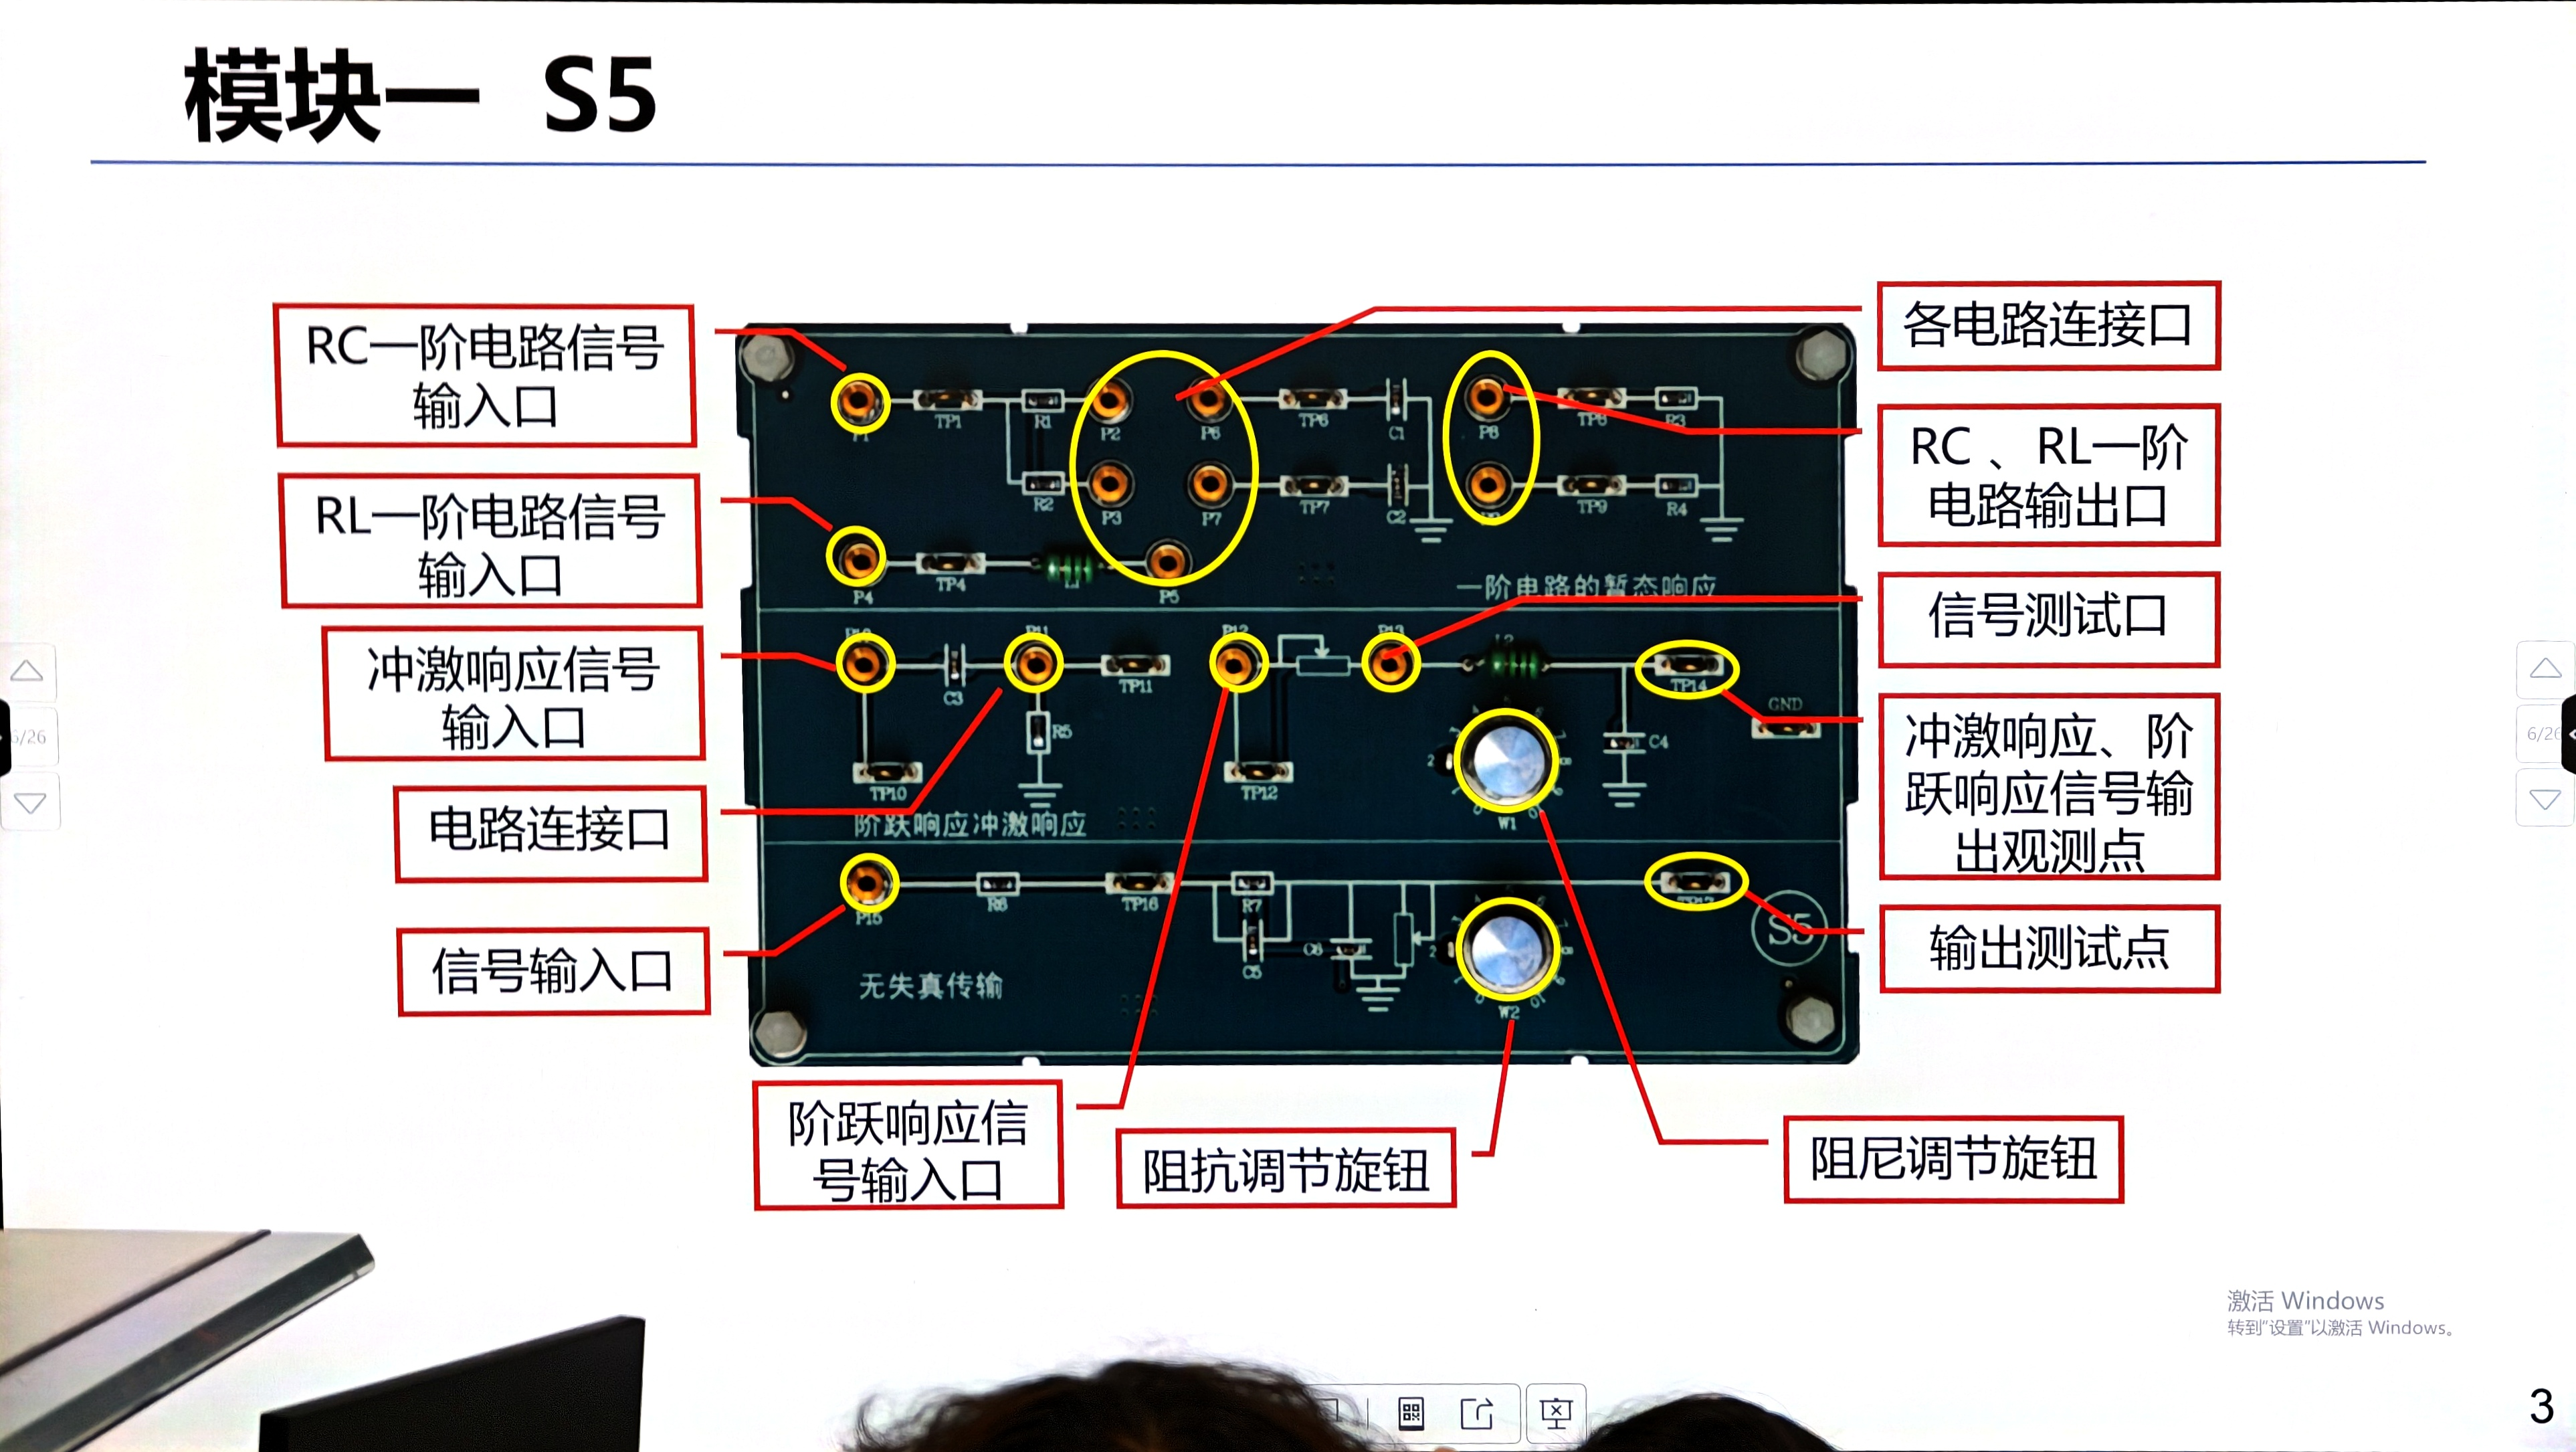
\includegraphics[width=\linewidth]{./2. impluse_step/figures/s5.jpg}
        \caption{一阶网络模块 S5}
        \label{fig:s5_sub}
    \end{subfigure}
    
    \caption{实验核心模块} % 整个图的总标题
    \label{fig:modules}
\end{figure}

\section{实验原理}

\subsection{基本概念}
对于一个线性时不变（LTI）系统，其动态特性可以通过系统对特定输入信号的响应来描述。其中，最基本的两种响应是单位冲激响应和单位阶跃响应。

\begin{itemize}
    \item \textbf{单位冲激响应}: 当输入信号为单位冲激函数 $\delta(t)$ 时，系统产生的零状态响应称为单位冲激响应，记为 $h(t)$。如图 \ref{fig:impulse_response} 所示。
    \item \textbf{单位阶跃响应}: 当输入信号为单位阶跃函数 $u(t)$ 时，系统产生的零状态响应称为单位阶跃响应，记为 $g(t)$。如图 \ref{fig:step_response} 所示。
\end{itemize}

冲激响应与阶跃响应之间存在密切的微积分关系：阶跃响应是冲激响应的积分，而冲激响应是阶跃响应的导数。
\[ g(t) = \int_{0}^{t} h(\tau) d\tau \quad \Leftrightarrow \quad h(t) = \frac{d g(t)}{dt} \]

\begin{figure}[htbp]
    \centering
    \begin{subfigure}{0.48\textwidth}
        \centering
        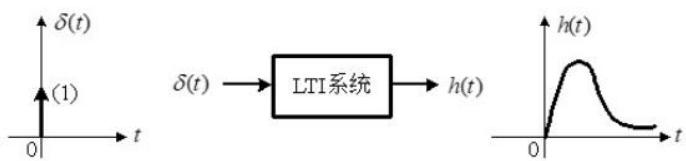
\includegraphics[width=\linewidth]{./2. impluse_step/figures/fig_impulse_response.png}
        \caption{冲激响应示意图}
        \label{fig:impulse_response}
    \end{subfigure}
    \hfill
    \begin{subfigure}{0.48\textwidth}
        \centering
        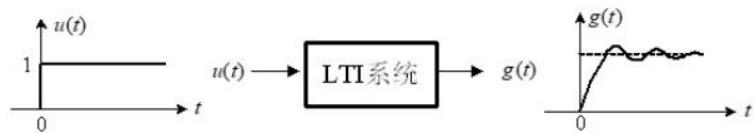
\includegraphics[width=\linewidth]{./2. impluse_step/figures/fig_step_response.png}
        \caption{阶跃响应示意图}
        \label{fig:step_response}
    \end{subfigure}
    \caption{LTI 系统的基本响应}
    \label{fig:lti_responses}
\end{figure}


\subsection{RLC 串联电路的响应分析}
本实验研究的对象是二阶 RLC 串联电路，其阶跃响应与冲激响应的电路连接如图 \ref{fig:rlc_circuits} 所示。根据电阻 $R$、电感 $L$ 和电容 $C$ 的取值不同，系统的响应会呈现出三种不同的状态：
\begin{enumerate}
    \item \textbf{过阻尼状态}: 当 $R > 2\sqrt{\frac{L}{C}}$ 时，响应曲线无振荡，缓慢上升至稳态值。
    \item \textbf{临界阻尼状态}: 当 $R = 2\sqrt{\frac{L}{C}}$ 时，响应以最快的速度到达稳态值且无超调。
    \item \textbf{欠阻尼状态}: 当 $R < 2\sqrt{\frac{L}{C}}$ 时，响应曲线将出现振荡和超调现象。
\end{enumerate}

\begin{figure}[htbp]
    \centering
    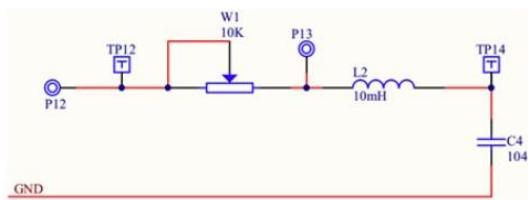
\includegraphics[width=0.4\textwidth]{./2. impluse_step/figures/fig_rlc_circuits.png}
    \caption{RLC 串联电路连接示意图}
    \label{fig:rlc_circuits}
\end{figure}


\subsection{动态性能指标}
对于欠阻尼二阶系统的阶跃响应，通常使用一系列动态性能指标来衡量其响应的快速性和稳定性，如图 \ref{fig:indicators} 所示。
\begin{description}
    \item[上升时间 ($t_r$)] 响应从稳态值的 10\% 上升到 90\% 所需的时间（或从0首次到达稳态值的时间）。
    \item[峰值时间 ($t_p$)] 响应从开始上升到第一个峰值点所需的时间。
    \item[调节时间 ($t_s$)] 响应进入并保持在稳态值的 $\pm 5\%$ (或 $\pm 2\%$) 误差带内所需的最短时间。
    \item[最大超调量 ($\delta_p$)] 响应的最大峰值 $y_{\max}$ 超出其稳态值 $y(\infty)$ 的百分比，计算公式为：
    \[ \delta_p = \frac{y_{\max} - y(\infty)}{y(\infty)} \times 100\% \]
\end{description}

\begin{figure}[htbp]
    \centering
    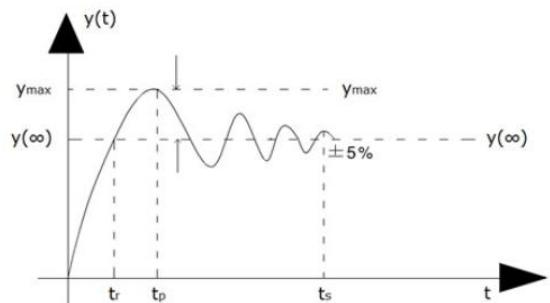
\includegraphics[width=0.4\textwidth]{./2. impluse_step/figures/fig_indicators.png}
    \caption{欠阻尼响应动态性能指标示意图}
    \label{fig:indicators}
\end{figure}

\section{实验数据与分析}

\subsection{波形观察与记录}
实验中，通过示波器观察并记录了阶跃响应和冲激响应在不同阻尼状态下的输入与输出波形，具体如下图所示。

% --- 阶跃响应波形图 ---
\begin{figure}[htbp]
    \centering
    \begin{subfigure}{0.32\textwidth}
        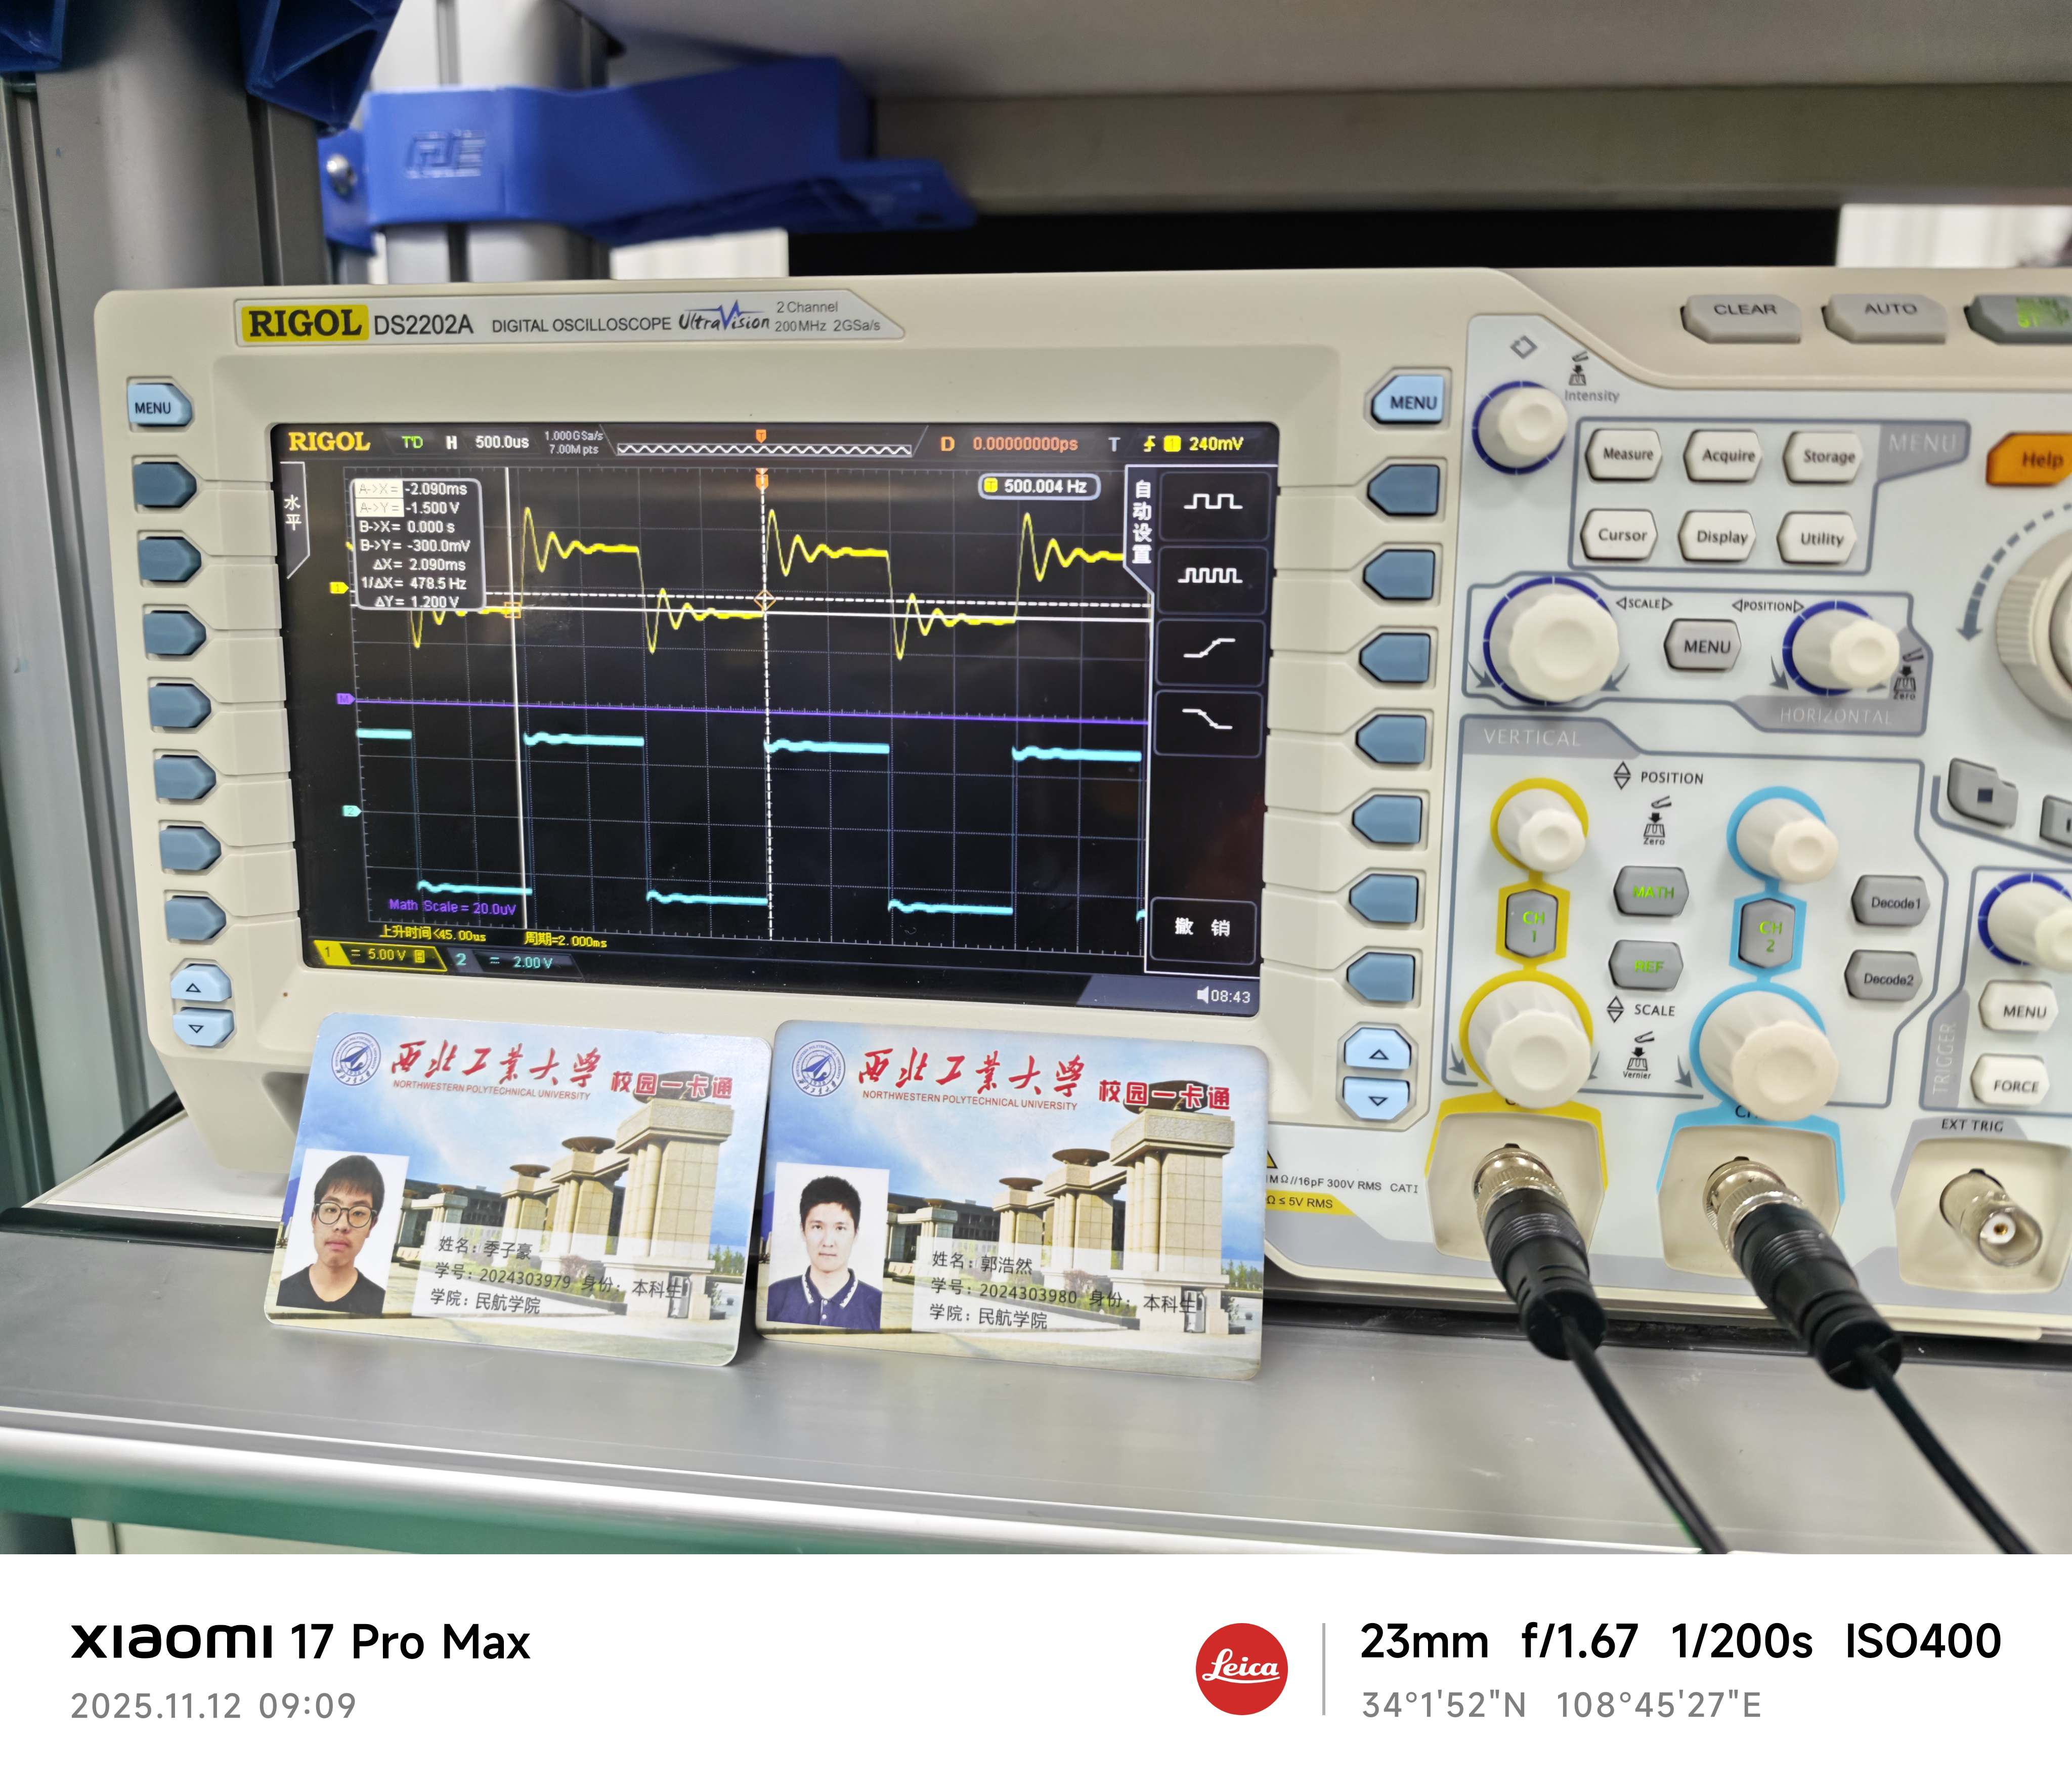
\includegraphics[width=\linewidth]{./2. impluse_step/figures/step_underdamped.jpg}
        \caption{欠阻尼状态}
        \label{fig:step_under}
    \end{subfigure}
    \hfill
    \begin{subfigure}{0.32\textwidth}
        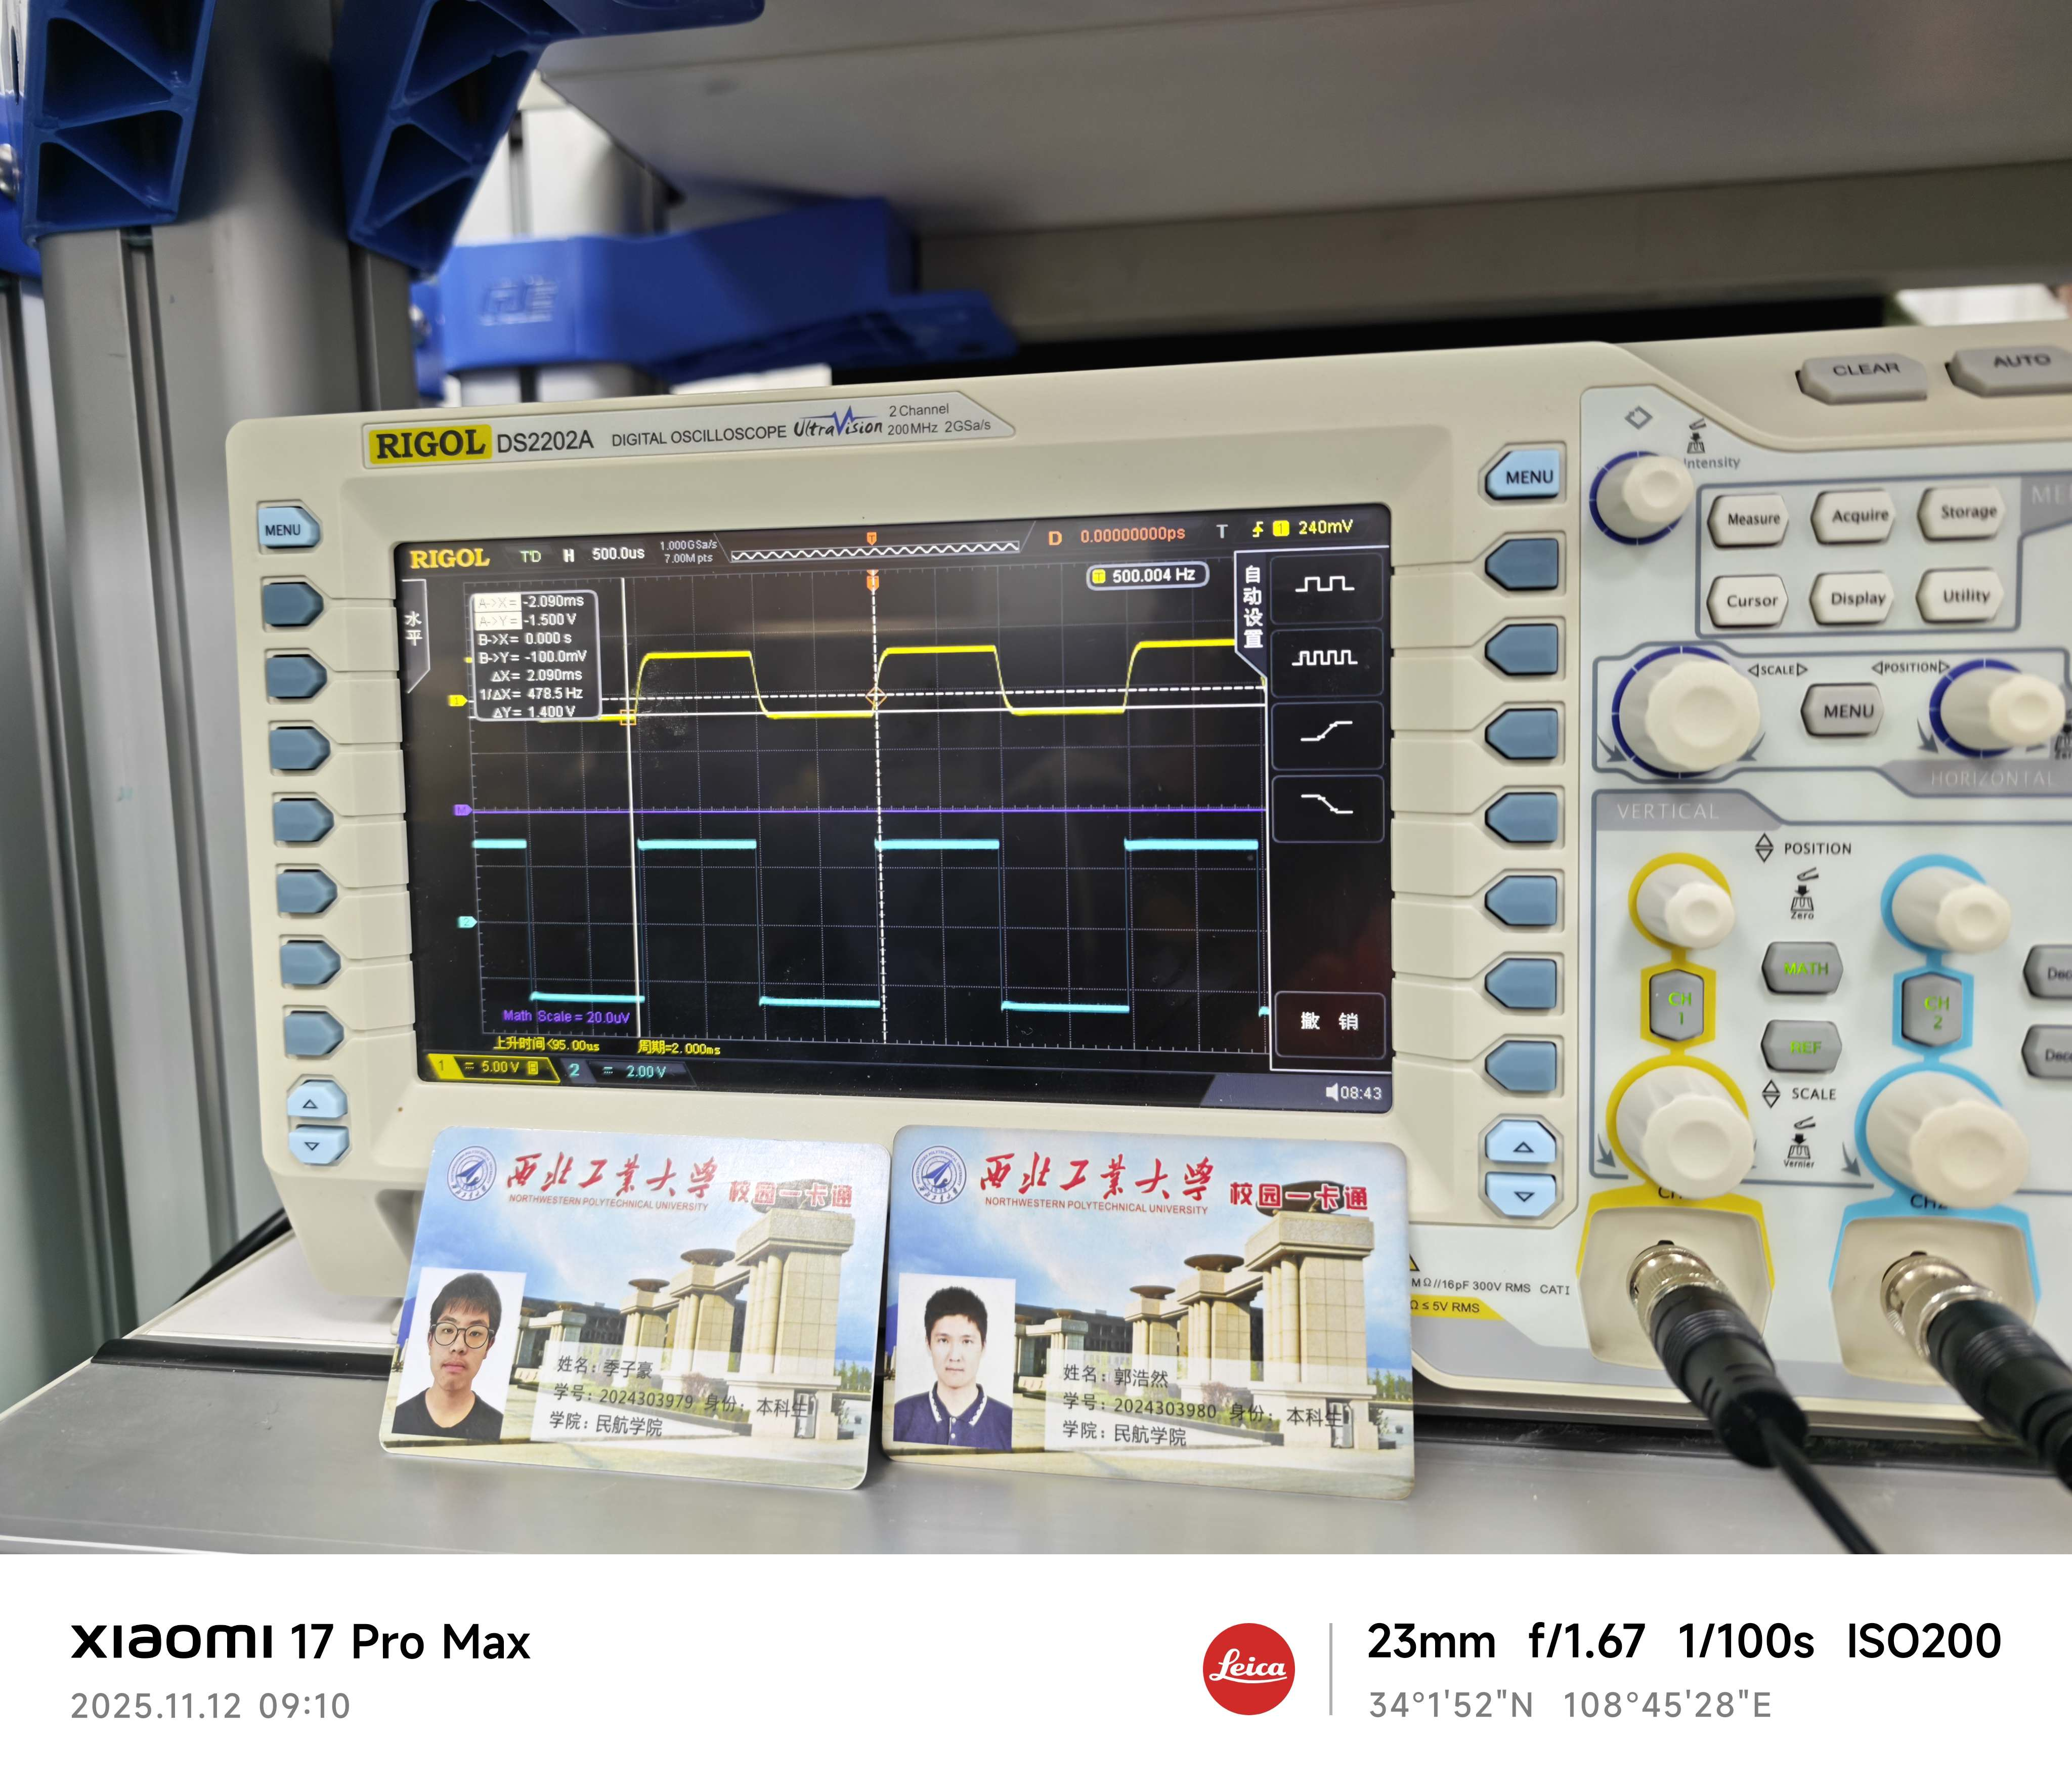
\includegraphics[width=\linewidth]{./2. impluse_step/figures/step_critical.jpg}
        \caption{临界阻尼状态}
        \label{fig:step_critical}
    \end{subfigure}
    \hfill
    \begin{subfigure}{0.32\textwidth}
        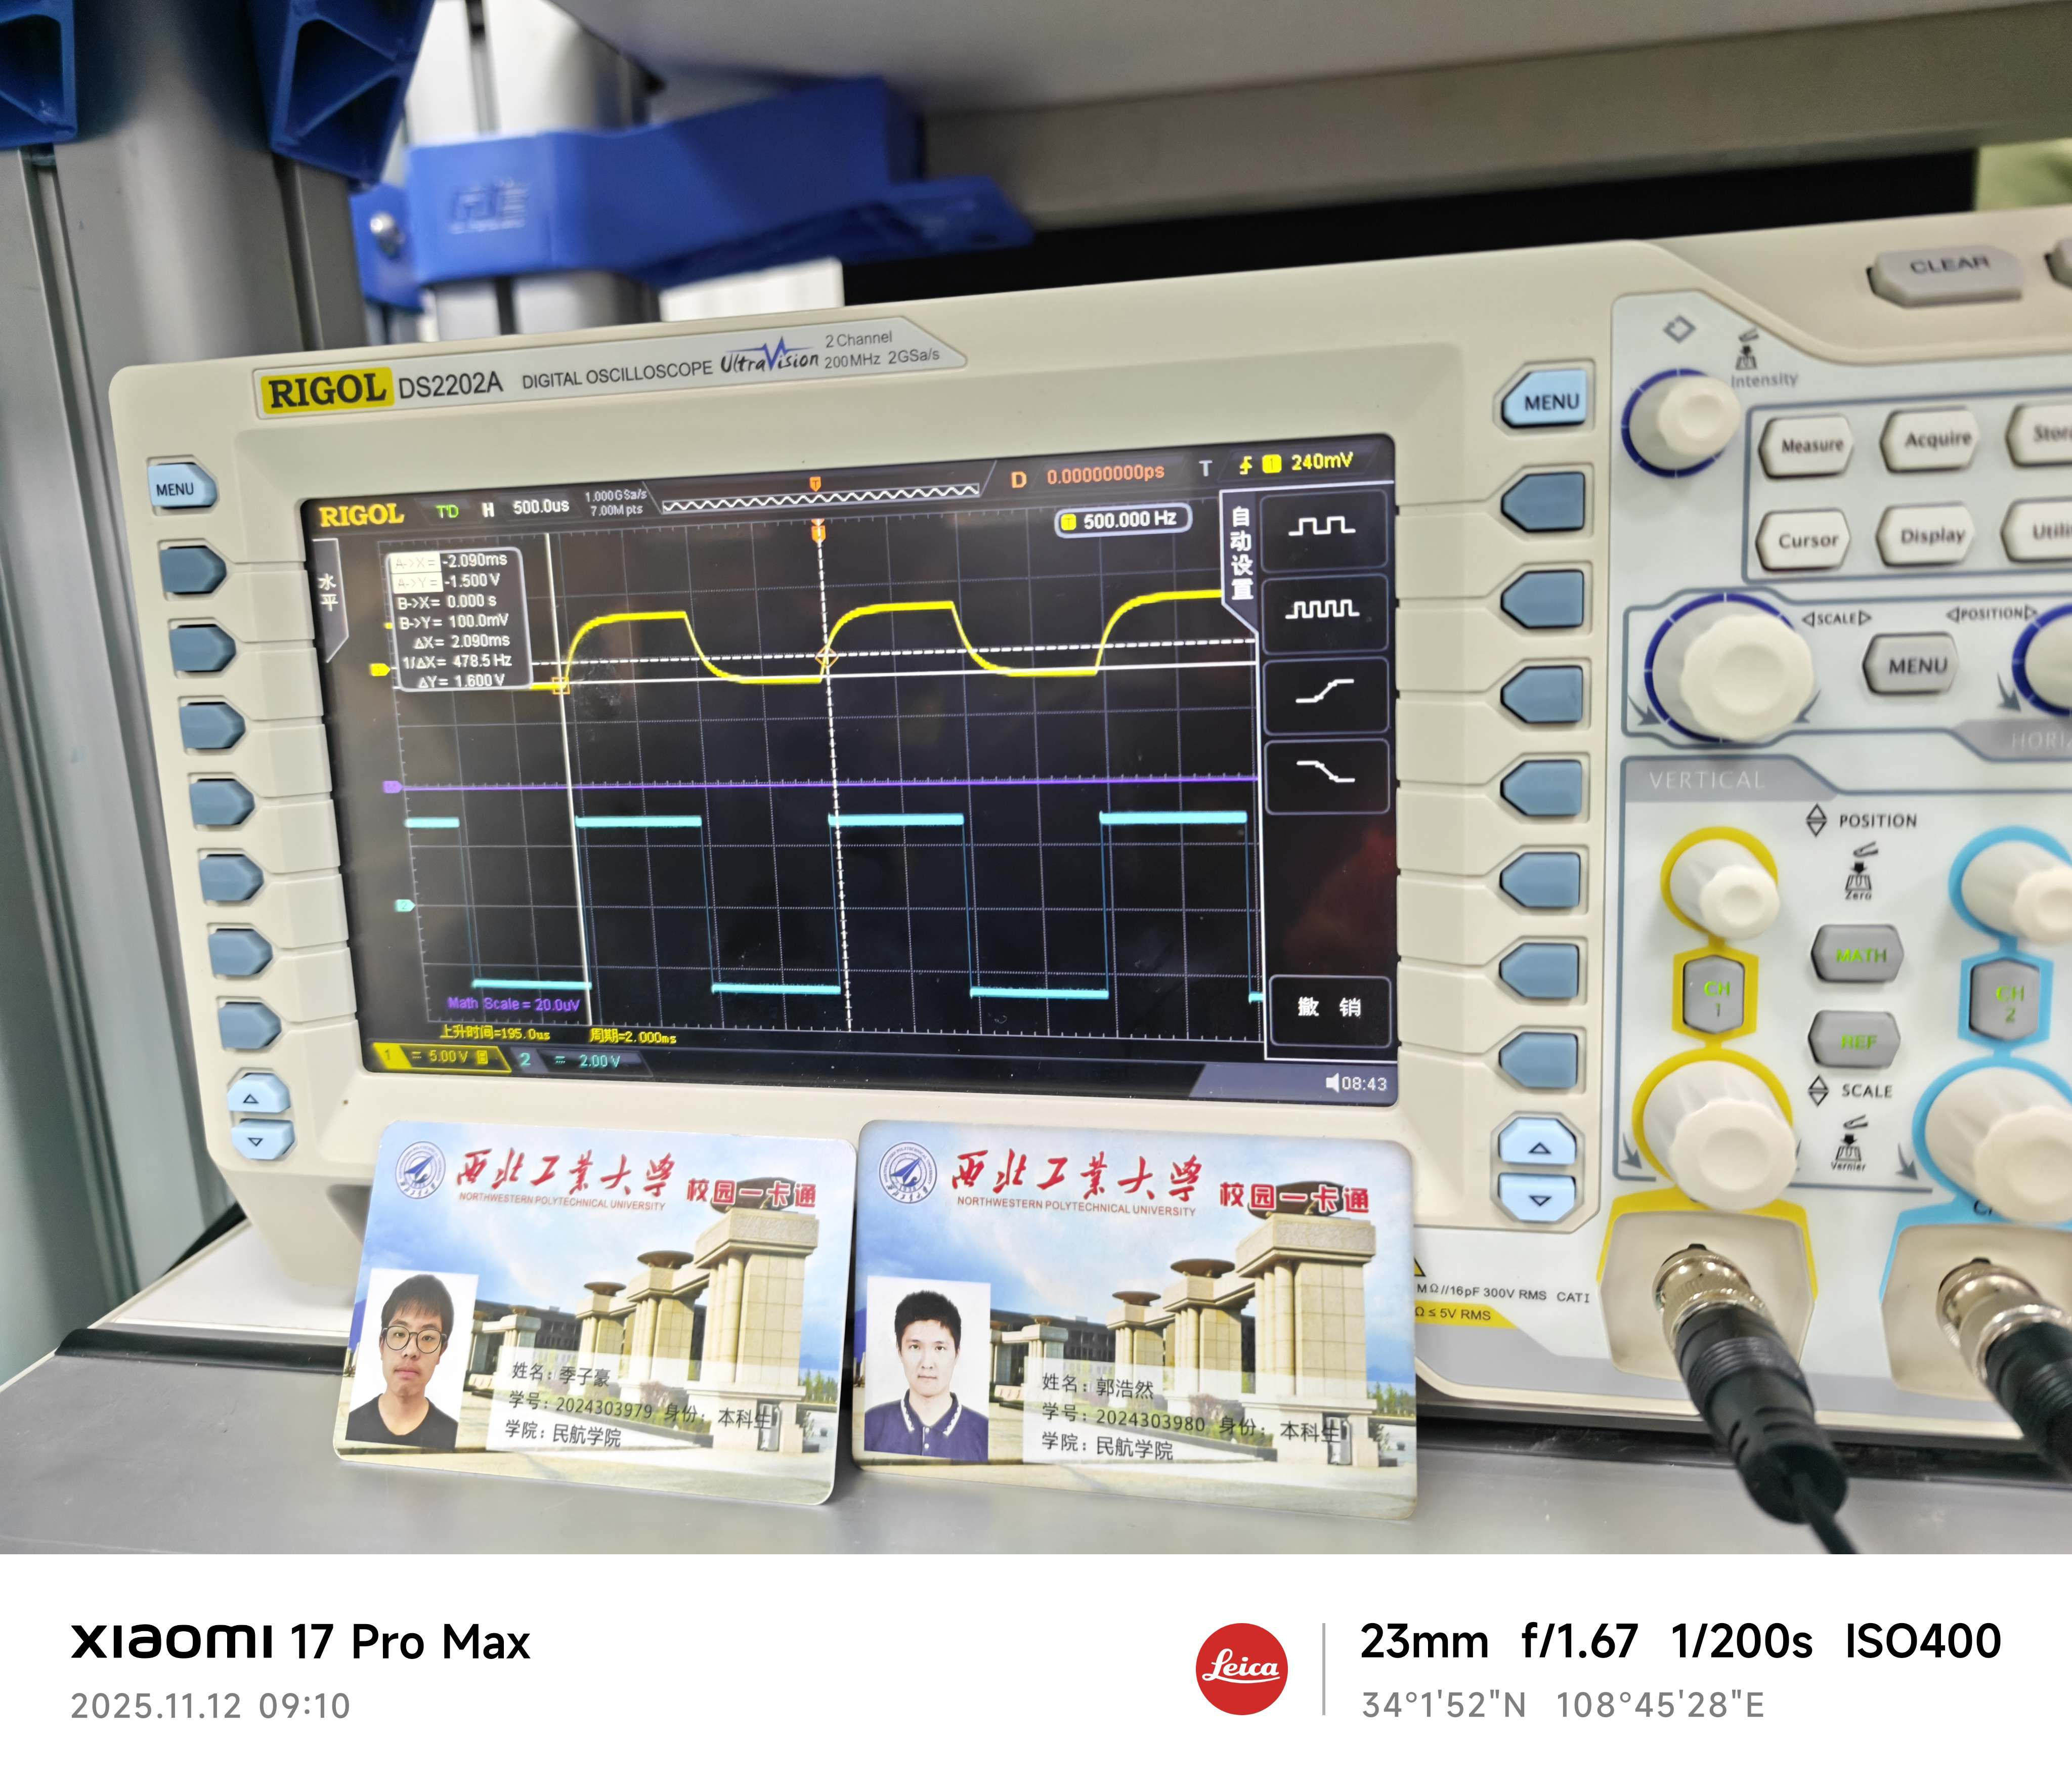
\includegraphics[width=\linewidth]{./2. impluse_step/figures/step_overdamped.jpg}
        \caption{过阻尼状态}
        \label{fig:step_over}
    \end{subfigure}
    \caption{阶跃响应在不同阻尼状态下的示波器波形}
    \label{fig:step_waveforms}
\end{figure}

% --- 冲激响应波形图 ---
\begin{figure}[htbp]
    \centering
    \begin{subfigure}{0.32\textwidth}
        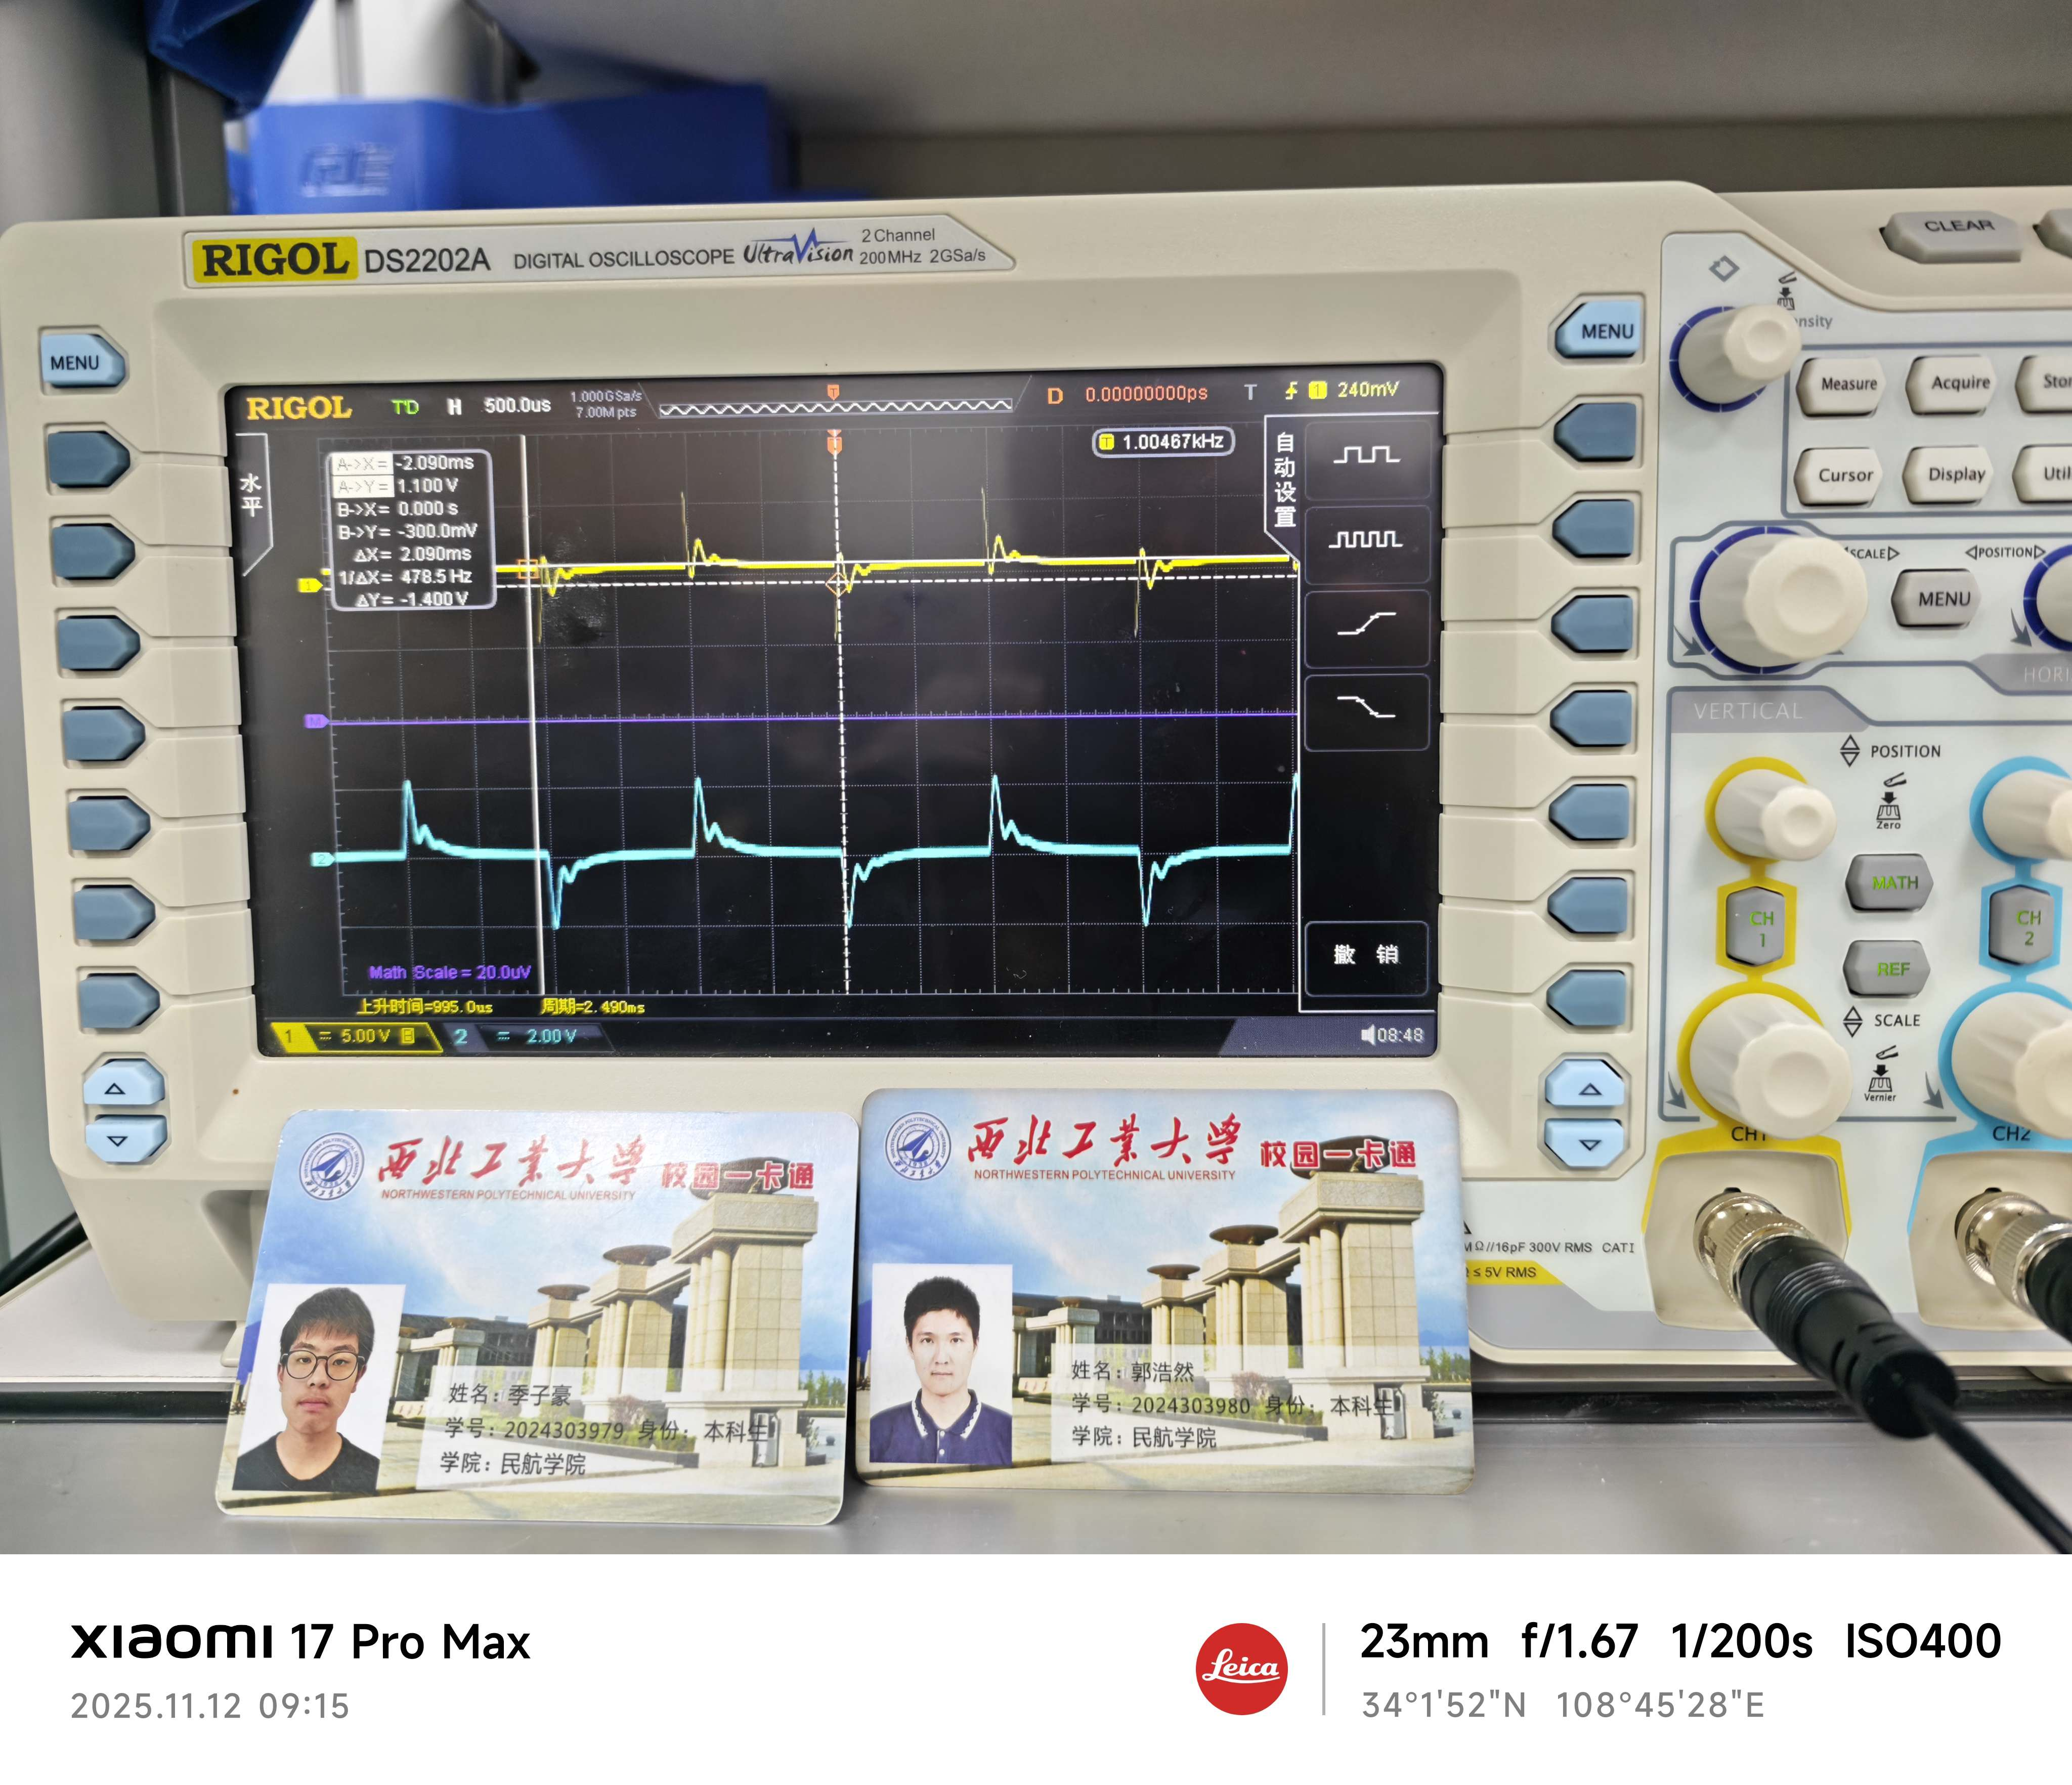
\includegraphics[width=\linewidth]{./2. impluse_step/figures/impulse_underdamped.jpg}
        \caption{欠阻尼状态}
        \label{fig:impulse_under}
    \end{subfigure}
    \hfill
    \begin{subfigure}{0.32\textwidth}
        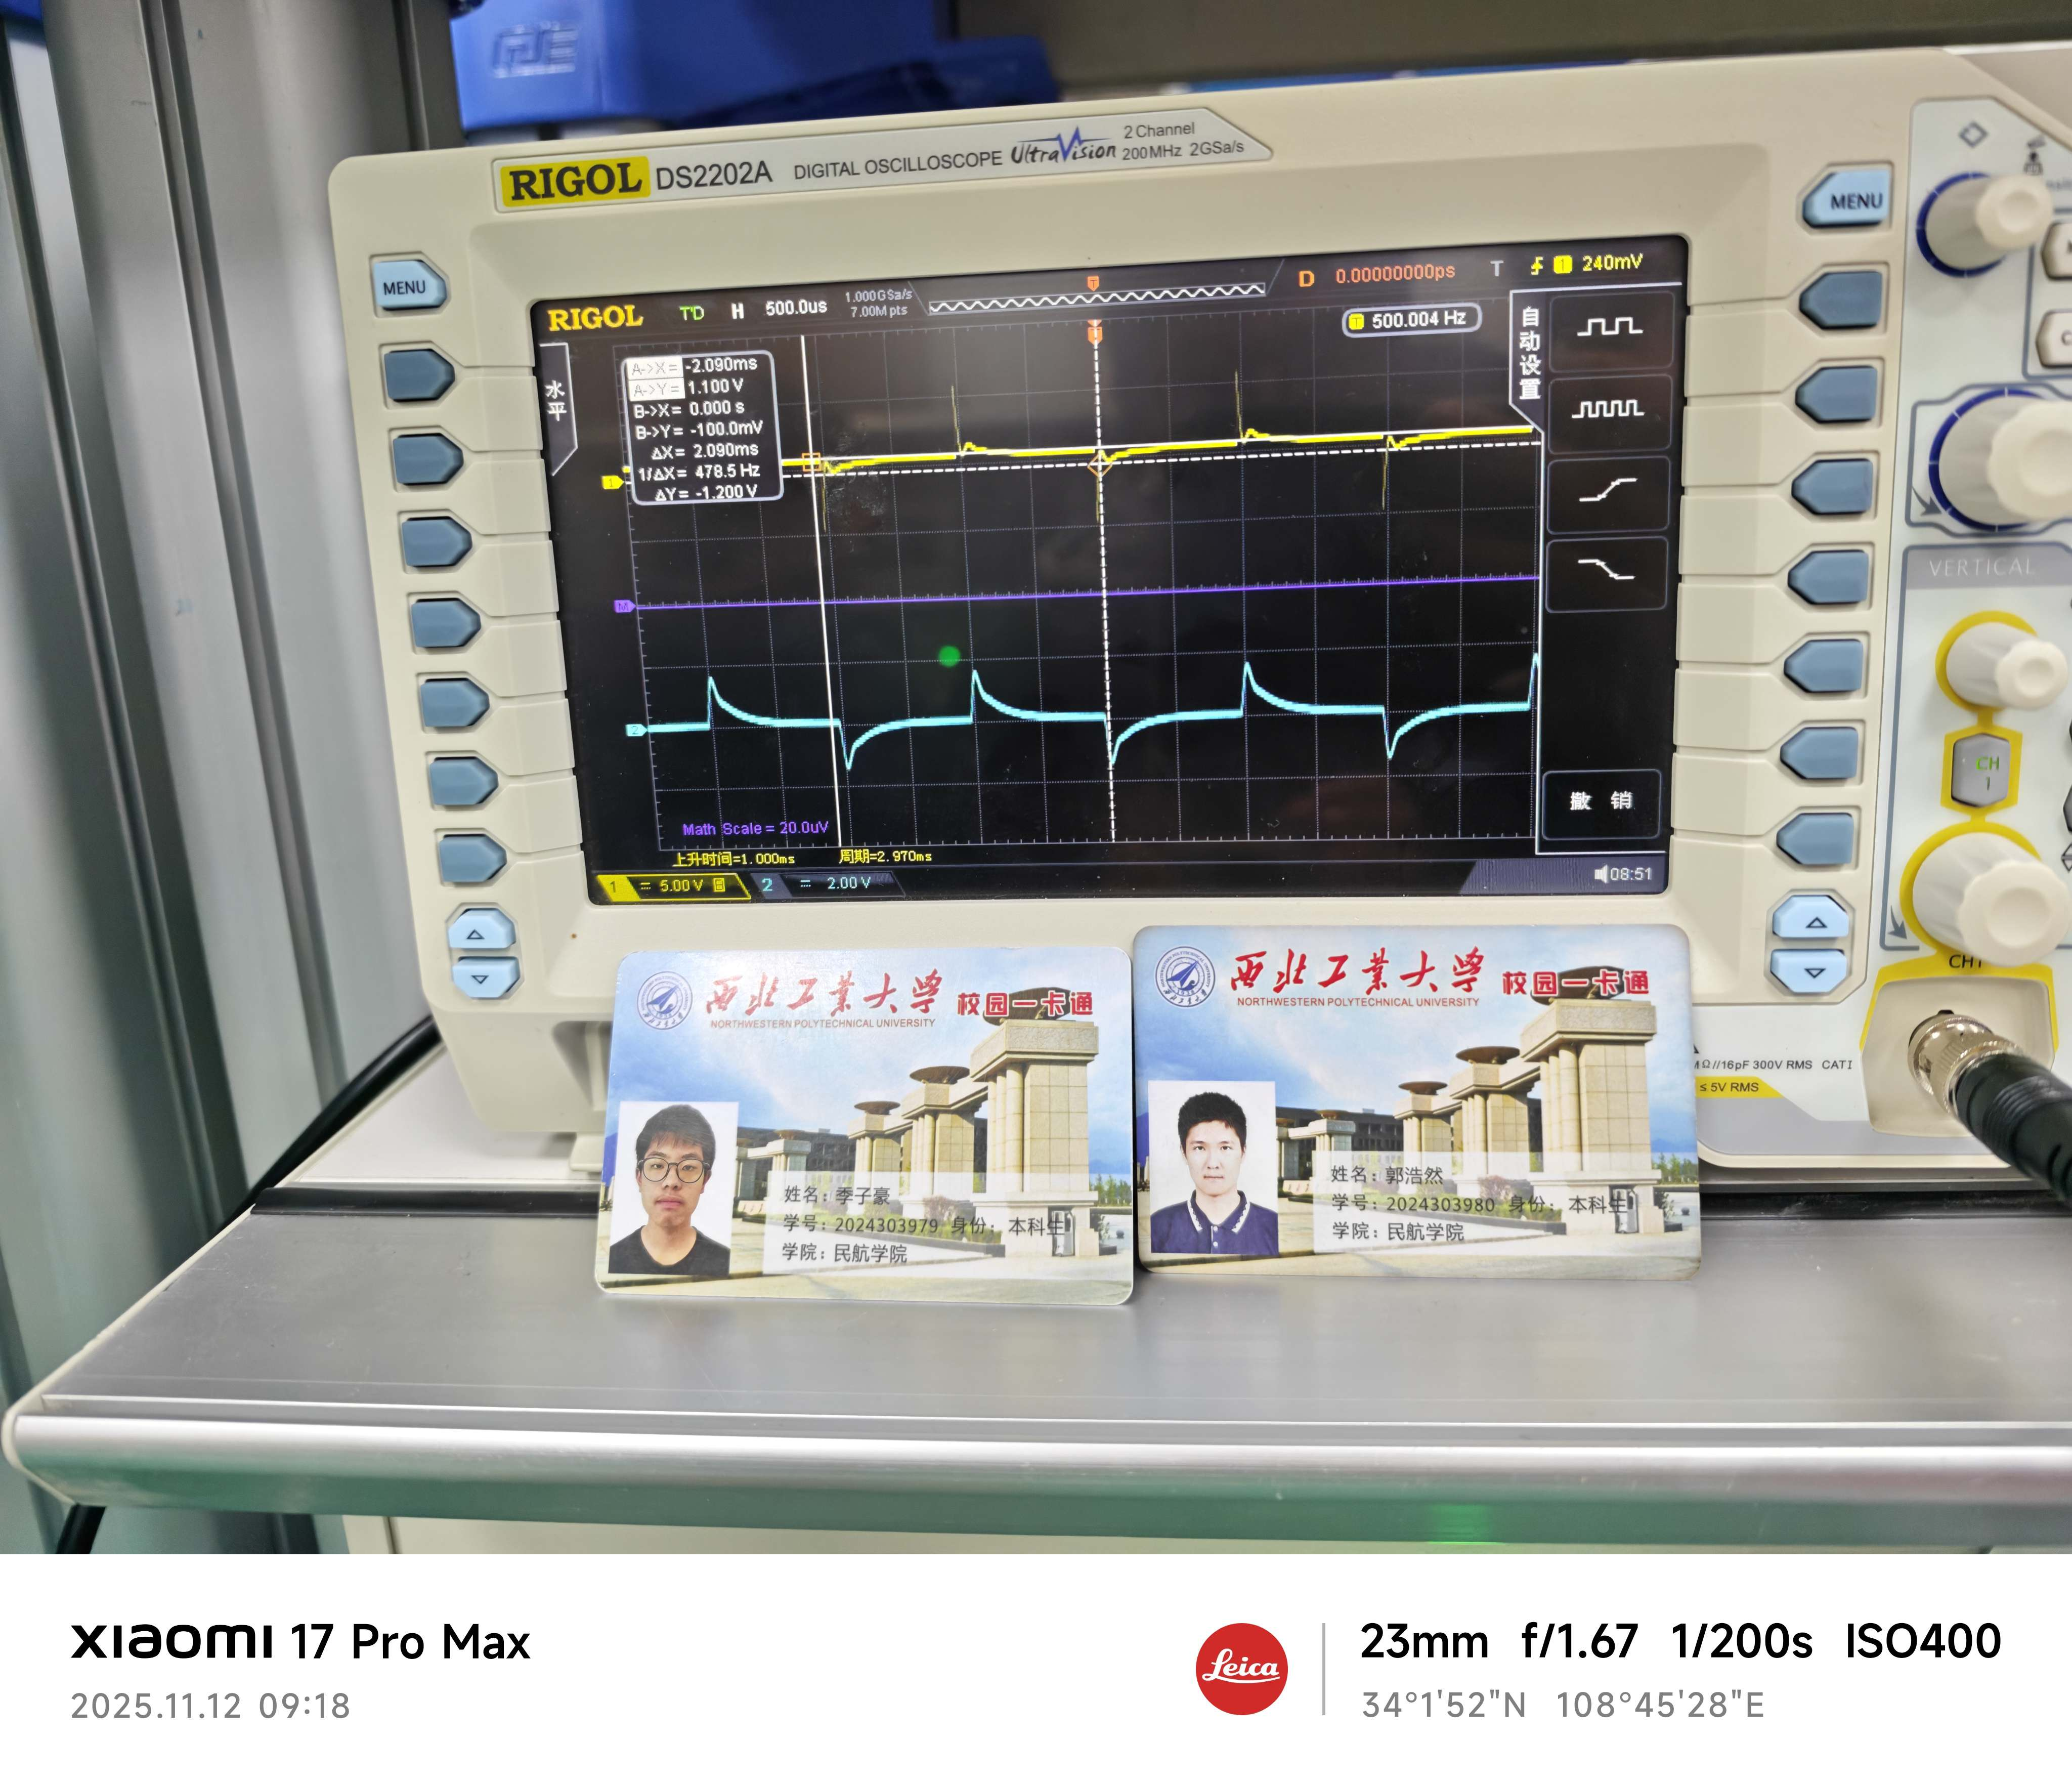
\includegraphics[width=\linewidth]{./2. impluse_step/figures/impulse_critical.jpg}
        \caption{临界阻尼状态}
        \label{fig:impulse_critical}
    \end{subfigure}
    \hfill
    \begin{subfigure}{0.32\textwidth}
        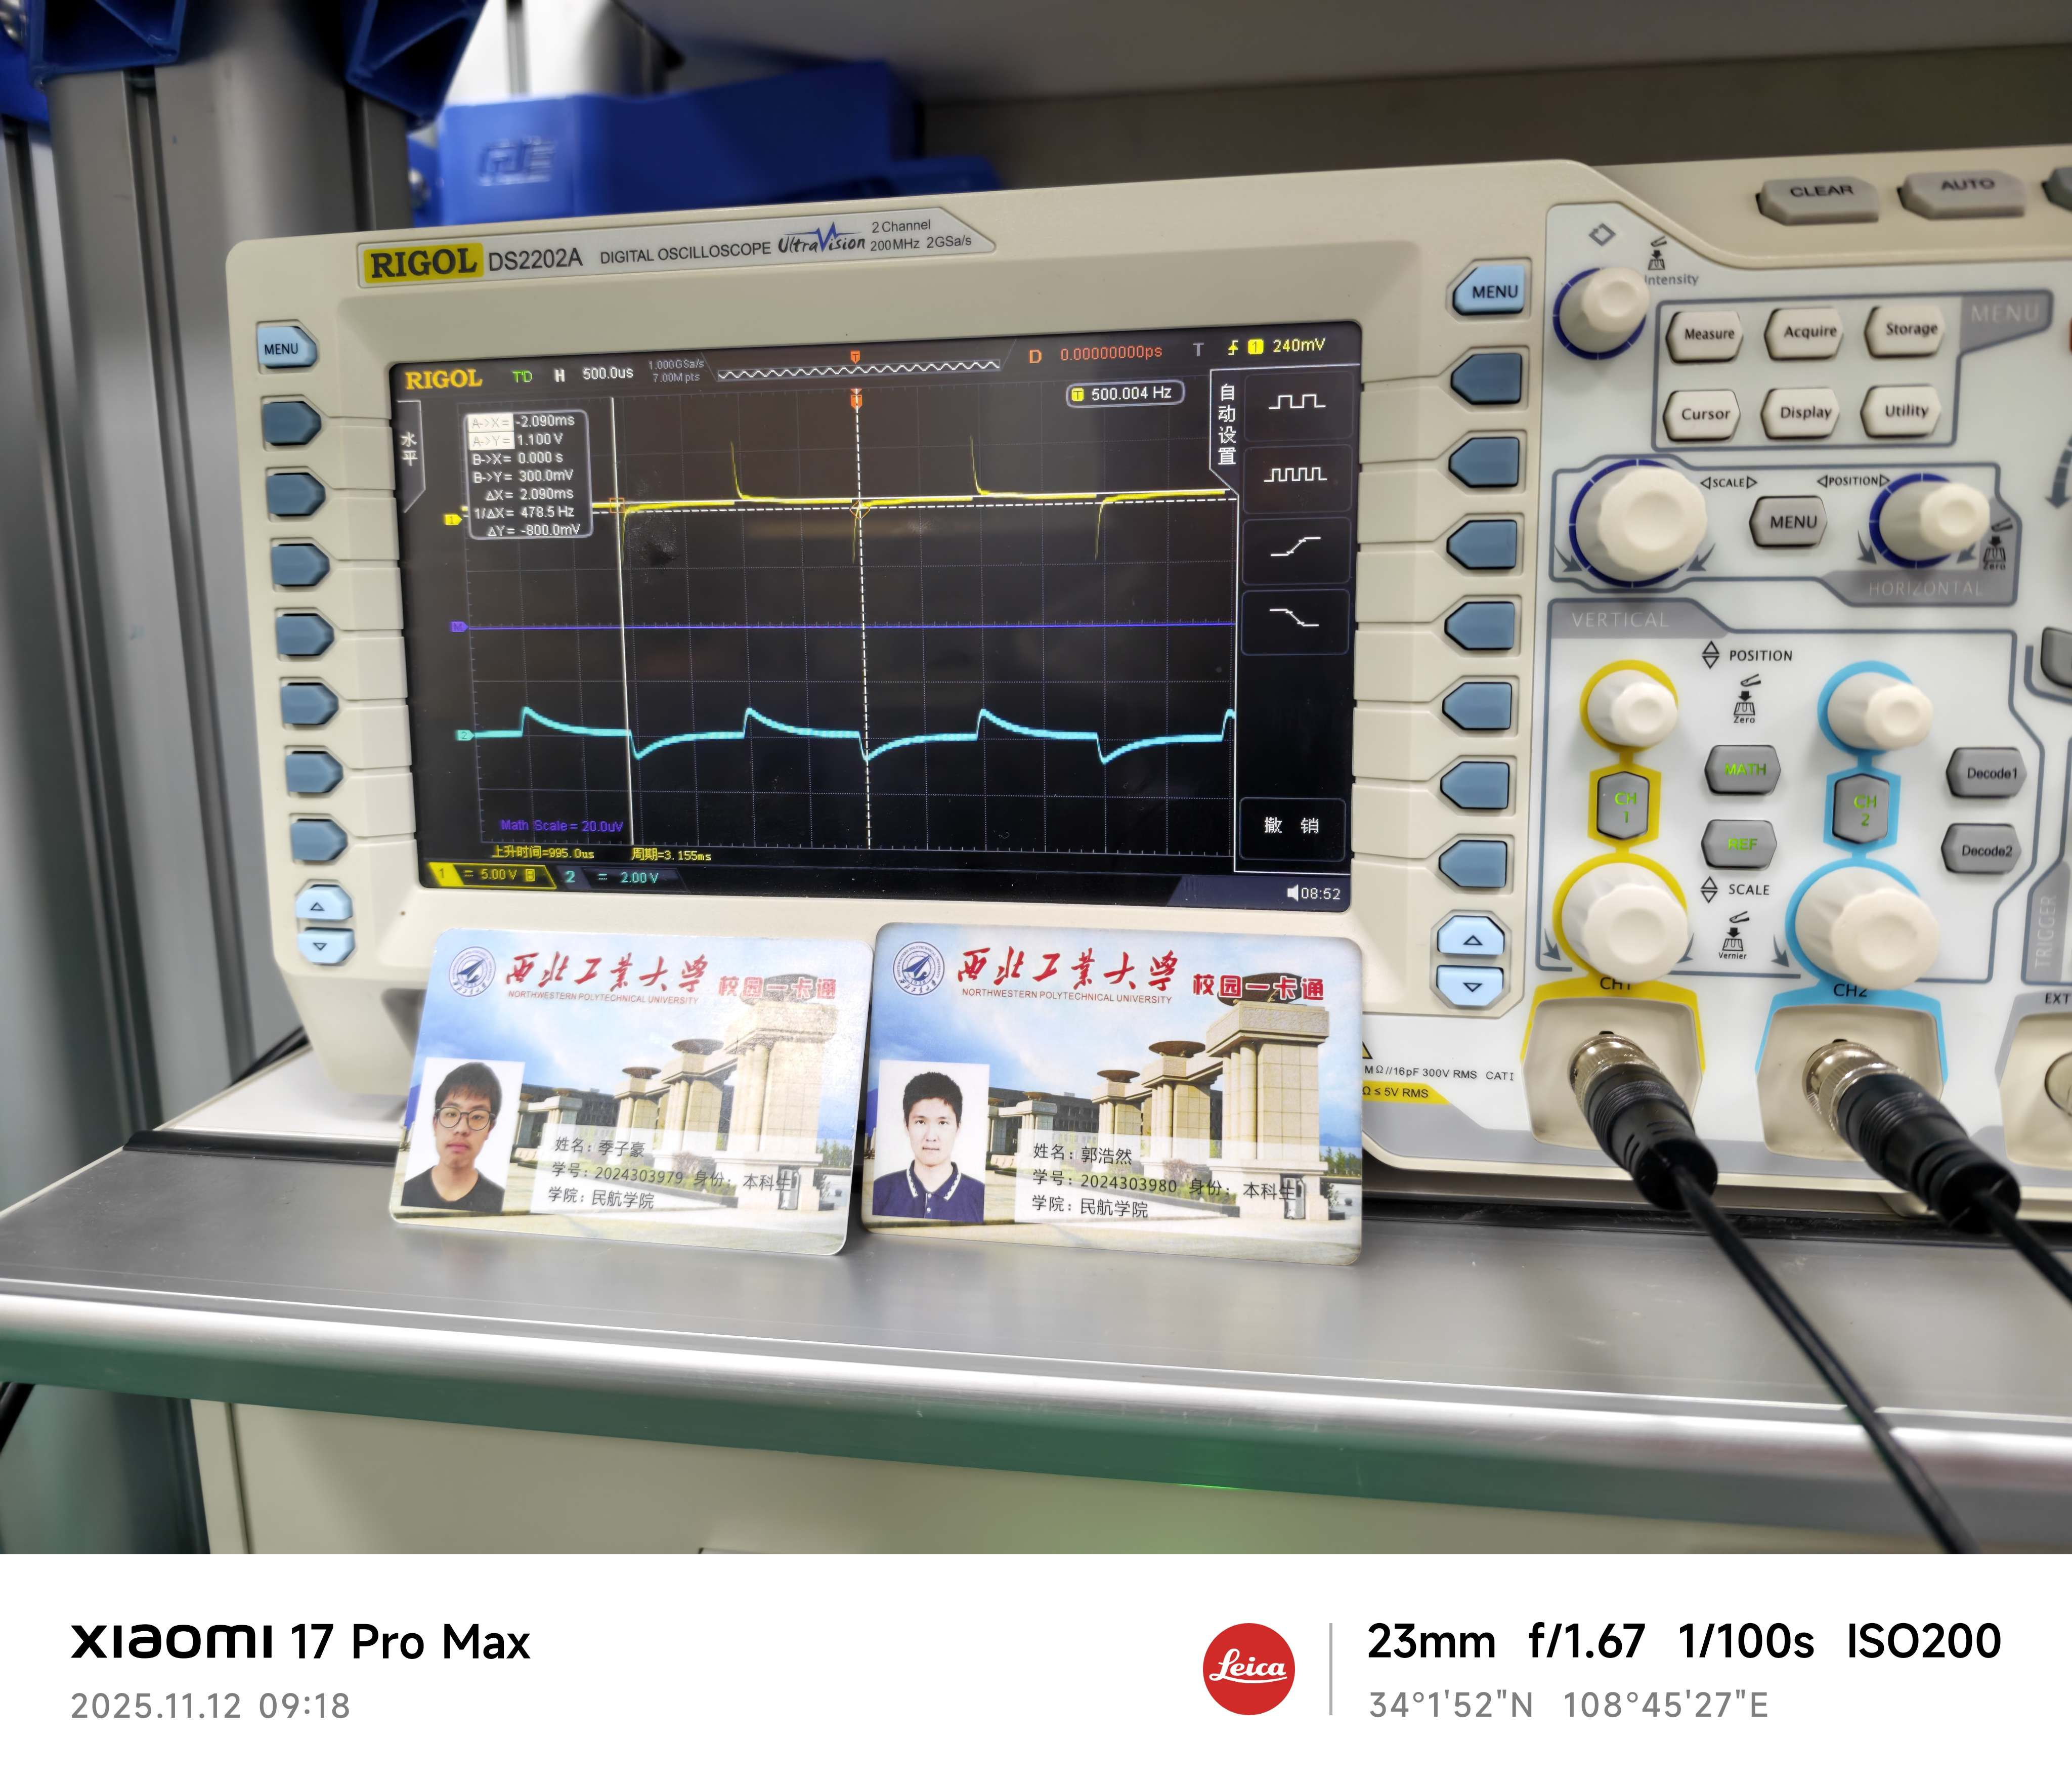
\includegraphics[width=\linewidth]{./2. impluse_step/figures/impulse_overdamped.jpg}
        \caption{过阻尼状态}
        \label{fig:impulse_over}
    \end{subfigure}
    \caption{冲激响应在不同阻尼状态下的示波器波形}
    \label{fig:impulse_waveforms}
\end{figure}


\subsection{参数测量数据}
在观察波形的同时，对各状态下的关键参数进行了测量，详细数据记录在表 \ref{tab:step_data} 和表 \ref{tab:impulse_data} 中。

% --- 阶跃响应数据表 (代码与之前相同) ---
\begin{table}[htbp]
    \centering
    \caption{阶跃响应参数测量数据}
    \label{tab:step_data}
    \renewcommand{\arraystretch}{1.5}
    \begin{tabular}{l c c c}
        \toprule
        \textbf{测量项目} & \textbf{欠阻尼状态} & \textbf{临界阻尼状态} & \textbf{过阻尼状态} \\
        \midrule
        电阻测量值 R & \SI{11.6}{\ohm} & \SI{484}{\ohm} & \SI{1109}{\ohm} \\
        \addlinespace
        TP12 激励波形 & \makecell{A = \SI{975}{\milli\volt} \\ T = \SI{2}{\milli\second} \\ $T_1$ = \SI{1}{\milli\second}} & \makecell{A = \SI{975}{\milli\volt} \\ T = \SI{2}{\milli\second} \\ $T_1$ = \SI{1}{\milli\second}} & \makecell{A = \SI{975}{\milli\volt} \\ T = \SI{2}{\milli\second} \\ $T_1$ = \SI{1}{\milli\second}} \\
        \addlinespace
        TP14 响应波形 & \makecell{A = \SI{969}{\milli\volt} \\ T = \SI{2}{\milli\second} \\ $T_1$ = \SI{1}{\milli\second} \\ $\tau$ = \SI{34}{\micro\second}} & \makecell{A = \SI{962}{\milli\volt} \\ T = \SI{2}{\milli\second} \\ $T_1$ = \SI{1}{\milli\second} \\ $\tau$ = \SI{70}{\micro\second}} & \makecell{A = \SI{940}{\milli\volt} \\ T = \SI{2}{\milli\second} \\ $T_1$ = \SI{1}{\milli\second} \\ $\tau$ = \SI{286}{\micro\second}} \\
        \bottomrule
    \end{tabular}
\end{table}

% --- 冲激响应数据表 (代码与之前相同) ---
\begin{table}[htbp]
    \centering
    \caption{冲激响应参数测量数据}
    \label{tab:impulse_data}
    \renewcommand{\arraystretch}{1.5}
    \begin{tabular}{l c c c}
        \toprule
        \textbf{测量项目} & \textbf{欠阻尼状态} & \textbf{临界阻尼状态} & \textbf{过阻尼状态} \\
        \midrule
        电阻测量值 R & \SI{3.0}{\ohm} & \SI{287}{\ohm} & \SI{1100}{\ohm} \\
        \addlinespace
        TP12 激励波形 & \makecell{A = \SI{1.988}{\volt} \\ T = \SI{2}{\milli\second} \\ $T_1$ = \SI{1}{\milli\second}} & \makecell{A = \SI{1.988}{\volt} \\ T = \SI{2}{\milli\second} \\ $T_1$ = \SI{1}{\milli\second}} & \makecell{A = \SI{1.988}{\volt} \\ T = \SI{2}{\milli\second} \\ $T_1$ = \SI{1}{\milli\second}} \\
        \addlinespace
        TP14 响应波形 & \makecell{A = \SI{820}{\milli\volt} \\ T = \SI{2}{\milli\second} \\ $T_1$ = \SI{1}{\milli\second} \\ $\tau$ = \SI{20}{\micro\second}} & \makecell{A = \SI{270}{\milli\volt} \\ T = \SI{2}{\milli\second} \\ $T_1$ = \SI{1}{\milli\second} \\ $\tau$ = \SI{90}{\micro\second}} & \makecell{A = \SI{220}{\milli\volt} \\ T = \SI{2}{\milli\second} \\ $T_1$ = \SI{1}{\milli\second} \\ $\tau$ = \SI{120}{\micro\second}} \\
        \bottomrule
    \end{tabular}
\end{table}


\subsection{综合分析}
结合图 \ref{fig:step_waveforms}、\ref{fig:impulse_waveforms} 所示的波形和表 \ref{tab:step_data}、\ref{tab:impulse_data} 的数据可以看出：
\begin{enumerate}
    \item \textbf{电阻与阻尼状态的关系：} 实验测得的电阻值 R 随着系统从欠阻尼、临界阻尼到过阻尼状态转变而显著增大。这与实验原理中 $R$ 与 $2\sqrt{L/C}$ 的大小关系完全吻合，验证了电阻是影响本 RLC 电路阻尼状态的关键参数。
    \item \textbf{阶跃响应分析：} 如图 \ref{fig:step_waveforms} 所示，在欠阻尼状态下，响应波形出现了明显的过冲和振荡；在临界阻尼状态下，波形最快达到稳定且无过冲；在过阻尼状态下，响应非常平缓，无过冲但上升时间最长。这与表 \ref{tab:step_data} 中响应时间常数 $\tau$ 从 \SI{34}{\micro\second} 增加到 \SI{286}{\micro\second} 的趋势一致。
    \item \textbf{冲激响应分析：} 如图 \ref{fig:impulse_waveforms} 所示，阻尼对冲激响应的峰值影响剧烈。随着阻尼增加，响应峰值迅速衰减，恢复到零的时间也相应变化。这说明阻尼越大，系统对瞬时冲击的能量耗散越快，抑制作用越强，与表 \ref{tab:impulse_data} 中峰值幅度从 \SI{820}{\milli\volt} 锐减至 \SI{220}{\milli\volt} 的数据相符。
\end{enumerate}
综上所述，实验波形和测量数据清晰地展示了二阶 RLC 电路在不同阻尼条件下对阶跃和冲激信号的响应特性，与理论预期高度一致。

\section{信号的 Matlab 仿真与分析}

本章节展示了使用 Matlab 对一系列信号进行仿真和变换的结果。

\begin{figure}[H]
    \centering
    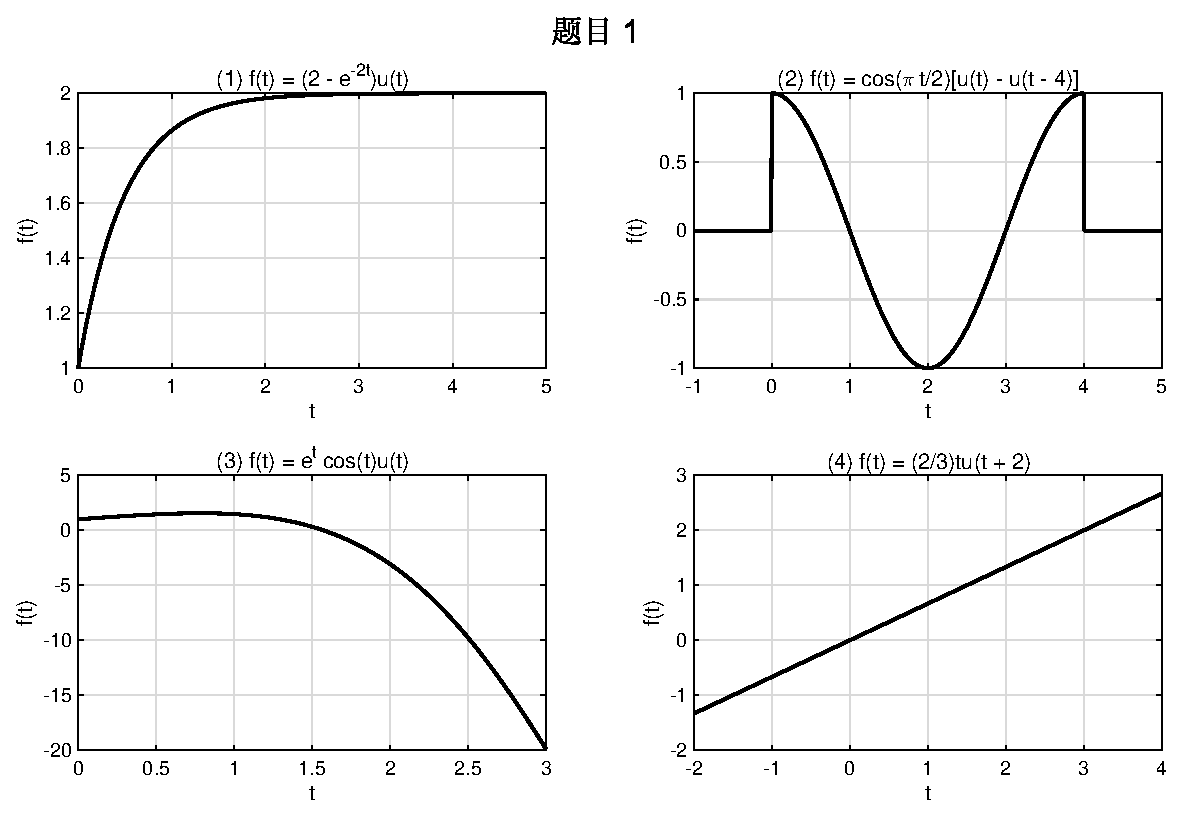
\includegraphics[width=0.7\textwidth]{./2. impluse_step/figures/T1.eps}
    \caption{题目 1：连续时间信号波形}
    \label{fig:T1}
\end{figure}

\begin{figure}[H]
    \centering
    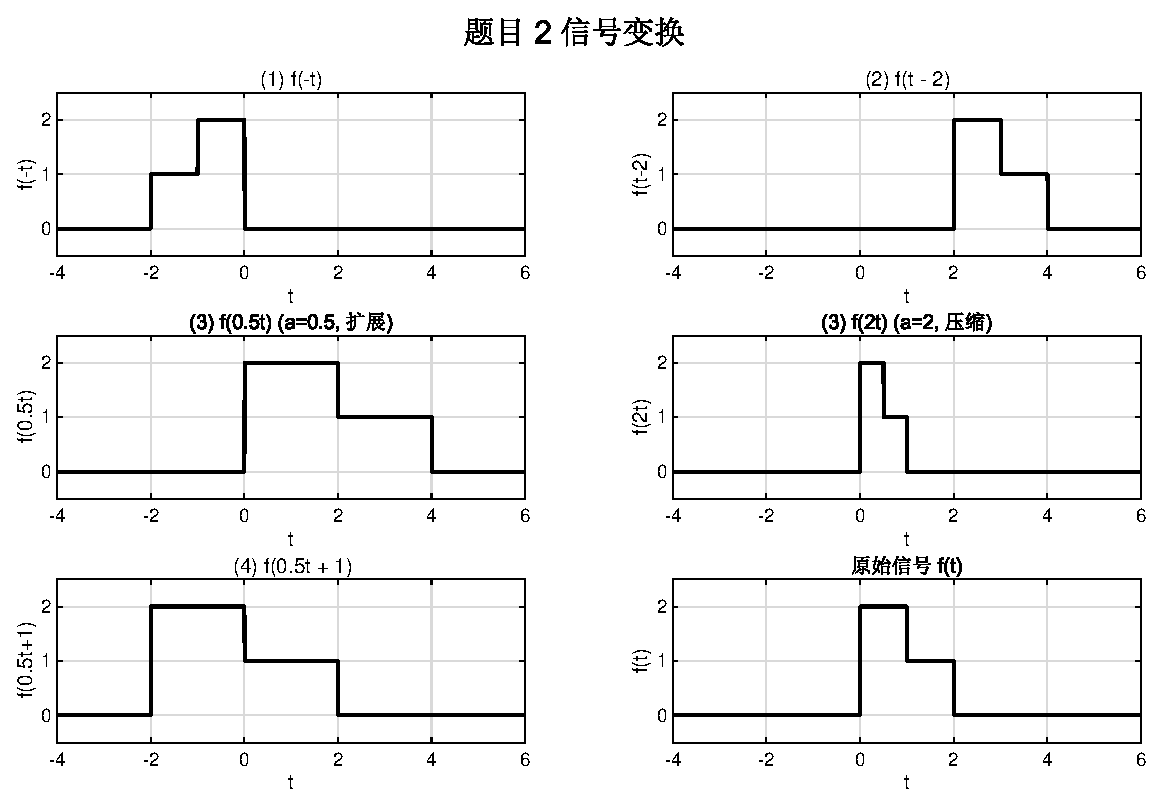
\includegraphics[width=0.8\textwidth]{./2. impluse_step/figures/T2.eps}
    \caption{题目 2：信号 f(t) 的基本变换}
    \label{fig:T2}
\end{figure}
\begin{figure}[H]
    \centering
    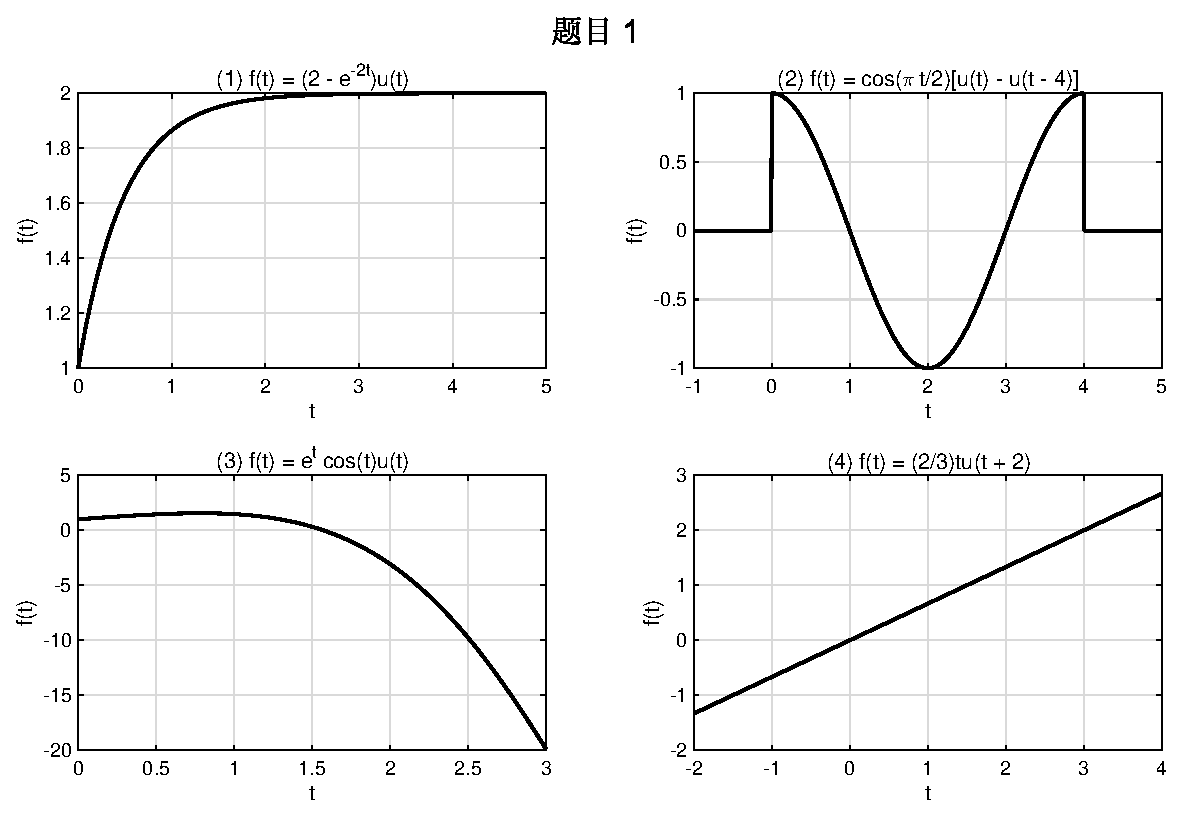
\includegraphics[width=0.8\textwidth]{./2. impluse_step/figures/T3.eps}
    \caption{题目 3：复信号 $f(t) = 2e^{j(t+\pi/4)}$ 的各分量}
    \label{fig:T3}
\end{figure}


\section{结论}
本次实验通过搭建 RLC 串联电路，成功观察并测量了二阶系统在不同阻尼条件下的阶跃响应与冲激响应，得出以下结论：

\begin{enumerate}
    \item \textbf{验证了阻尼理论：} 实验结果清晰地表明，电路的阻尼状态由电阻 R 的值决定。通过改变 R 值，可以使电路呈现出欠阻尼、临界阻尼和过阻尼三种不同的响应特性，这与 $R$ 和 $2\sqrt{L/C}$ 的理论关系完全一致。

    \item \textbf{掌握了响应特性：}
    \begin{itemize}
        \item \textbf{阶跃响应：} 欠阻尼状态响应速度快但伴有超调和振荡；临界阻尼状态响应速度最快且无超调，是理想的快速响应状态；过阻尼状态响应平稳无超调，但响应时间最长。
        \item \textbf{冲激响应：} 阻尼越大，系统对瞬时冲击的抑制能力越强，响应峰值越低，能量耗散越快。
    \end{itemize}

    \item \textbf{探究了响应关系：} 实验中通过将方波（近似阶跃信号）输入微分电路来获得冲激响应波形，直观地验证了冲激响应是阶跃响应的微分这一基本理论关系。

    \item \textbf{提升了测量技能：} 通过本次实验，熟练掌握了使用示波器观察动态波形、测量上升时间、峰值等动态性能指标的方法，并对二阶系统的时域分析有了更深刻的物理认识。
\end{enumerate}

% ===================================================================
% 第三章：连续时间系统模拟 (Origin: 3. convolution)
% ===================================================================
\chapter{连续时间系统模拟}

\section{实验目的}
\begin{enumerate}
    \item 了解基本运算器——比例放大器、加法器和积分器的电路结构和运算功能。
    \item 掌握用基本运算单元模拟连续时间一阶系统原理与测试方法。
\end{enumerate}

\section{实验器材}
\begin{enumerate}
    \item 双踪示波器 1台
    \item 数字万用表 1块
    \item 电压表及直流信号源模块 S1 1块
    \item 信号源及频率计模块 S2 1块
    \item 基本运算单元与连续系统模块 S9 1块
\end{enumerate}

\section{实验原理}

\subsection{线性系统的模拟}
系统的模拟就是用由基本运算单元组成的模拟装置来模拟实际的系统。这些实际系统可以是电的或非电的物理量系统，也可以是社会、经济和军事等非物理量系统。模拟装置可以与实际系统的内容完全不同，但是两者的微分方程完全相同，输入、输出关系即传输函数也完全相同。模拟装置的激励和响应是电物理量而实际系统的激励和响应不一定是电物理量，但它们之间的关系是一一对应的。所以，可以通过对模拟装置的研究来分析实际系统，最终达到一定条件下确定最佳参数的目的。

本实验所说的系统的模拟就是由基本的运算单元(放大器、加法器，积分器等)组成的模拟装置，来模拟实际系统的传输特性。

\subsection{三种基本运算电路}
\subsubsection{比例放大器}
电路如图\ref{fig:op-amp-prop}所示，其输入输出关系为：
\[ u_{0} = -\frac{R_{2}}{R_{1}} \cdot u_{1} \]

\begin{figure}[H]
    \centering
    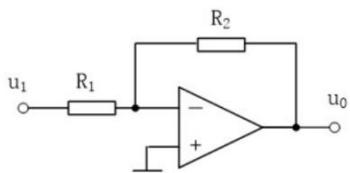
\includegraphics[width=0.4\textwidth]{./3. convolution/figures/fig3-1.png}
    \caption{比例放大电路连线示意图}
    \label{fig:op-amp-prop}
\end{figure}

\subsubsection{加法器}
电路如图\ref{fig:op-amp-add}所示，其输入输出关系为：
\[ u_{0} = -\frac{R_{2}}{R_{1}} (u_{1} + u_{2}) \]
当 $R_{1} = R_{2}$ 时，上式简化为 $u_{0} = -(u_{1} + u_{2})$。

\begin{figure}[H]
    \centering
    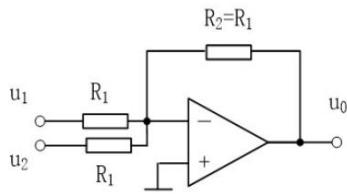
\includegraphics[width=0.4\textwidth]{./3. convolution/figures/fig3-2.png}
    \caption{加法器电路连线示意图}
    \label{fig:op-amp-add}
\end{figure}

\subsubsection{积分器}
电路如图\ref{fig:op-amp-int}所示，其输入输出关系为：
\[ u_{2} = -\frac{1}{RC}\int_{-\infty}^{t}u_{1}(\tau)d\tau \]

\begin{figure}[H]
    \centering
    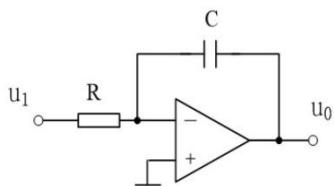
\includegraphics[width=0.4\textwidth]{./3. convolution/figures/fig3-3.png}
    \caption{积分器电路连接示意图}
    \label{fig:op-amp-int}
\end{figure}

\subsection{一阶系统的模拟}
一阶RC电路如图\ref{fig:rc-circuit}(a)所示，可用以下微分方程描述：
\[ \frac{\mathrm{d}y(t)}{\mathrm{d}t} + \frac{1}{RC} y(t) = \frac{1}{RC} x(t) \]
其模拟框图如图\ref{fig:rc-circuit}(b)和(c)所示，两者在数学关系上是等效的。对应的一阶系统模拟实验电路如图\ref{fig:rc-circuit}(d)所示。

\begin{figure}[H]
    \centering
    \begin{subfigure}[b]{0.38\textwidth}
        \centering
        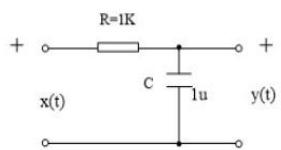
\includegraphics[width=\textwidth]{./3. convolution/figures/fig3-4a.png}
        \caption{一阶RC电路}
    \end{subfigure}
    \hfill
    \begin{subfigure}[b]{0.38\textwidth}
        \centering
        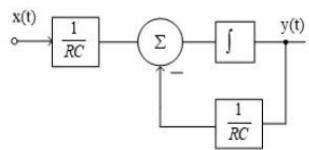
\includegraphics[width=\textwidth]{./3. convolution/figures/fig3-4b.png}
        \caption{模拟框图1}
    \end{subfigure}
    
    \vspace{1em} % 增加垂直间距
    
    \begin{subfigure}[b]{0.38\textwidth}
        \centering
        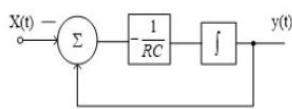
\includegraphics[width=\textwidth]{./3. convolution/figures/fig3-4c.png}
        \caption{模拟框图2 (等效)}
    \end{subfigure}
    \hfill
    \begin{subfigure}[b]{0.38\textwidth}
        \centering
        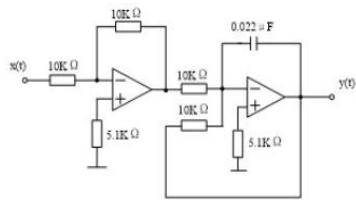
\includegraphics[width=\textwidth]{./3. convolution/figures/fig3-4d.png}
        \caption{一阶系统模拟实验电路}
    \end{subfigure}
    \caption{一阶RC电路及其模拟}
    \label{fig:rc-circuit}
\end{figure}

\section{实验步骤}
\subsection{任务一：基本运算器——加法器的观测}
\begin{enumerate}
    \item 模块关电，按如图\ref{fig:adder-exp-circuit}所示连接实验电路。
    \item 将模块S1的直流输出1(P1)和直流输出2(P2)分别接至加法器的 $u_{1}$ 和 $u_{2}$。模块开电，适当调节S1模块中的W1、W2，并记录P1和P2的电压值。
    \item 用万用表测量输出 $u_{0}$ 端电压。验证在反相加法器中，输出电压是否为两路输入电压之和取反相，完成表\ref{tab:adder-data}的记录。
    \item 将输入一改为峰峰值为 \SI{2}{\volt}、频率为 \SI{500}{\hertz} 的正弦波(方波)，再观察输入及输出波形，并完成记录。
\end{enumerate}

\begin{figure}[H]
    \centering
    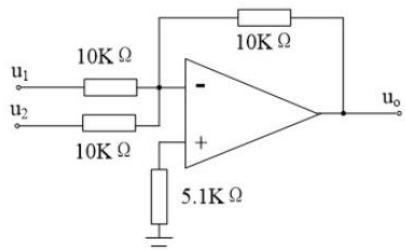
\includegraphics[width=0.4\textwidth]{./3. convolution/figures/fig3-6.png}
    \caption{加法器实验电路图}
    \label{fig:adder-exp-circuit}
\end{figure}

\subsection{任务二：基本运算器——比例放大器的观测}
\begin{enumerate}
    \item 模块关电，连接如图\ref{fig:prop-exp-circuit}所示实验电路。$R_1, R_2$可选择2组不同的电阻值以改变放大比例。
    \item 模块开电，信号发生器或模块产生幅度为 \SI{1}{\volt}、频率为 \SI{1}{\kilo\hertz} 的正弦波送入输入端，示波器同时观察并比较输入、输出波形，完成表\ref{tab:prop-data}的记录。
\end{enumerate}

\begin{figure}[H]
    \centering
    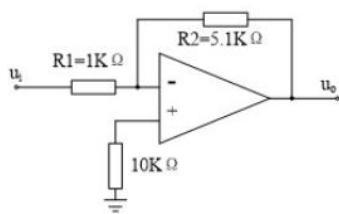
\includegraphics[width=0.4\textwidth]{./3. convolution/figures/fig3-7.png}
    \caption{比例放大器实验电路图}
    \label{fig:prop-exp-circuit}
\end{figure}

\subsection{任务三：基本运算器——积分器的观测}
为了防止低频信号增益过大，在电容两端并了一个 \SI{20}{\kilo\ohm} 电阻加以限制，同相输入端的 \SI{10}{\kilo\ohm} 电阻起到平衡电阻的作用。其输入输出关系为：
\[ u_{0}(t) = - \frac{1}{RC} \int_{t_{0}}^{t} u_{i}(\tau) \mathrm{d}\tau + u_{0}(t_{0}) \]
\begin{enumerate}
    \item 模块关电，连接如图\ref{fig:int-exp-circuit}所示实验电路。（\SI{20}{\kilo\ohm} 的电阻，可用两个 \SI{10}{\kilo\ohm} 的电路串联代替。）
    \item 模块开电，信号发生器或模块S2产生 $f = \SI{1}{\kilo\hertz}$ 的方波送入输入端，示波器同时观察输入、输出波形并比较自行完成实验数据记录。
\end{enumerate}

\begin{figure}[H]
    \centering
    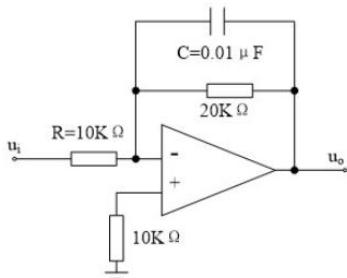
\includegraphics[width=0.3\textwidth]{./3. convolution/figures/fig3-8.png}
    \caption{积分器实验电路图}
    \label{fig:int-exp-circuit}
\end{figure}

\subsection{任务四：一阶RC电路的模拟}
图\ref{fig:rc-circuit}(a)为一阶RC电路，模块关电，按图\ref{fig:rc-circuit}(d)所示连接其一阶模拟电路。(阻容元件根据需要进行选择，\SI{0.022}{\micro\farad} 电容可由两个 \SI{0.01}{\micro\farad} 电容并联代替)。模块开电，将信号发生器产生的幅度为\SI{2}{\volt}、频率 \SI{1}{\kilo\hertz} 的方波送入一阶模拟电路输入端，用示波器观测输出电压波形，验证其模拟情况。

\begin{figure}[H]
    \centering
    \begin{subfigure}{0.48\textwidth}
        \centering
        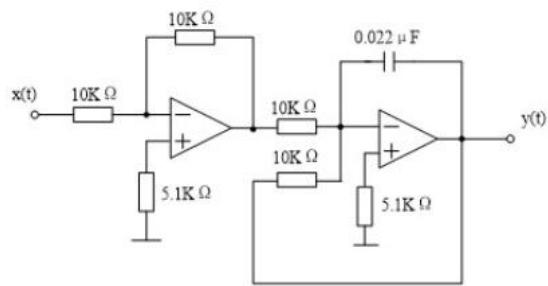
\includegraphics[width=\textwidth]{./3. convolution/figures/fig3-9a.png}
        \caption{模块实验电路图1}
    \end{subfigure}
    \hfill
    \begin{subfigure}{0.48\textwidth}
        \centering
        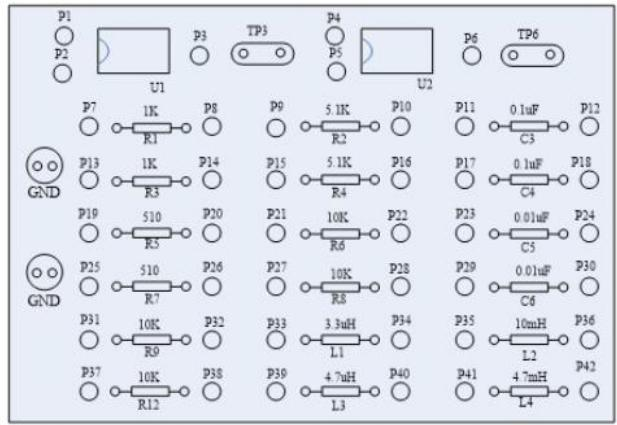
\includegraphics[width=\textwidth]{./3. convolution/figures/fig3-9b.png}
        \caption{模块实验电路图2}
    \end{subfigure}
    \caption{模块实验电路图}
    \label{fig:module-circuit}
\end{figure}

\section{实验数据}
\subsection{照片记录各基本运算器输入输出波形}

\subsubsection{加法器}

% 开启一个浮动体环境，用来包裹左右两部分
\begin{figure}[H]
    \centering
    
    % --- 左侧：表格 ---
    \begin{minipage}[c]{0.48\textwidth}
        \centering
        \captionof{table}{加法器直流输入测试数据}
        \label{tab:adder-data}
        \begin{tabular}{ccc}
            \toprule
            输入一 (\si{\volt}) & 输入二 (\si{\volt}) & 输出 (\si{\volt}) \\
            \midrule
            -2.2  & -2.73 & 4.94  \\
            2.00 & 5.08 & -7.07  \\
            1.66  & 1.03  & -2.7  \\
            \bottomrule
        \end{tabular}
    \end{minipage}
    \hfill % \hfill 负责在两个 minipage 之间撑开距离
    % --- 右侧：图片 ---
    \begin{minipage}[c]{0.48\textwidth}
        \centering
        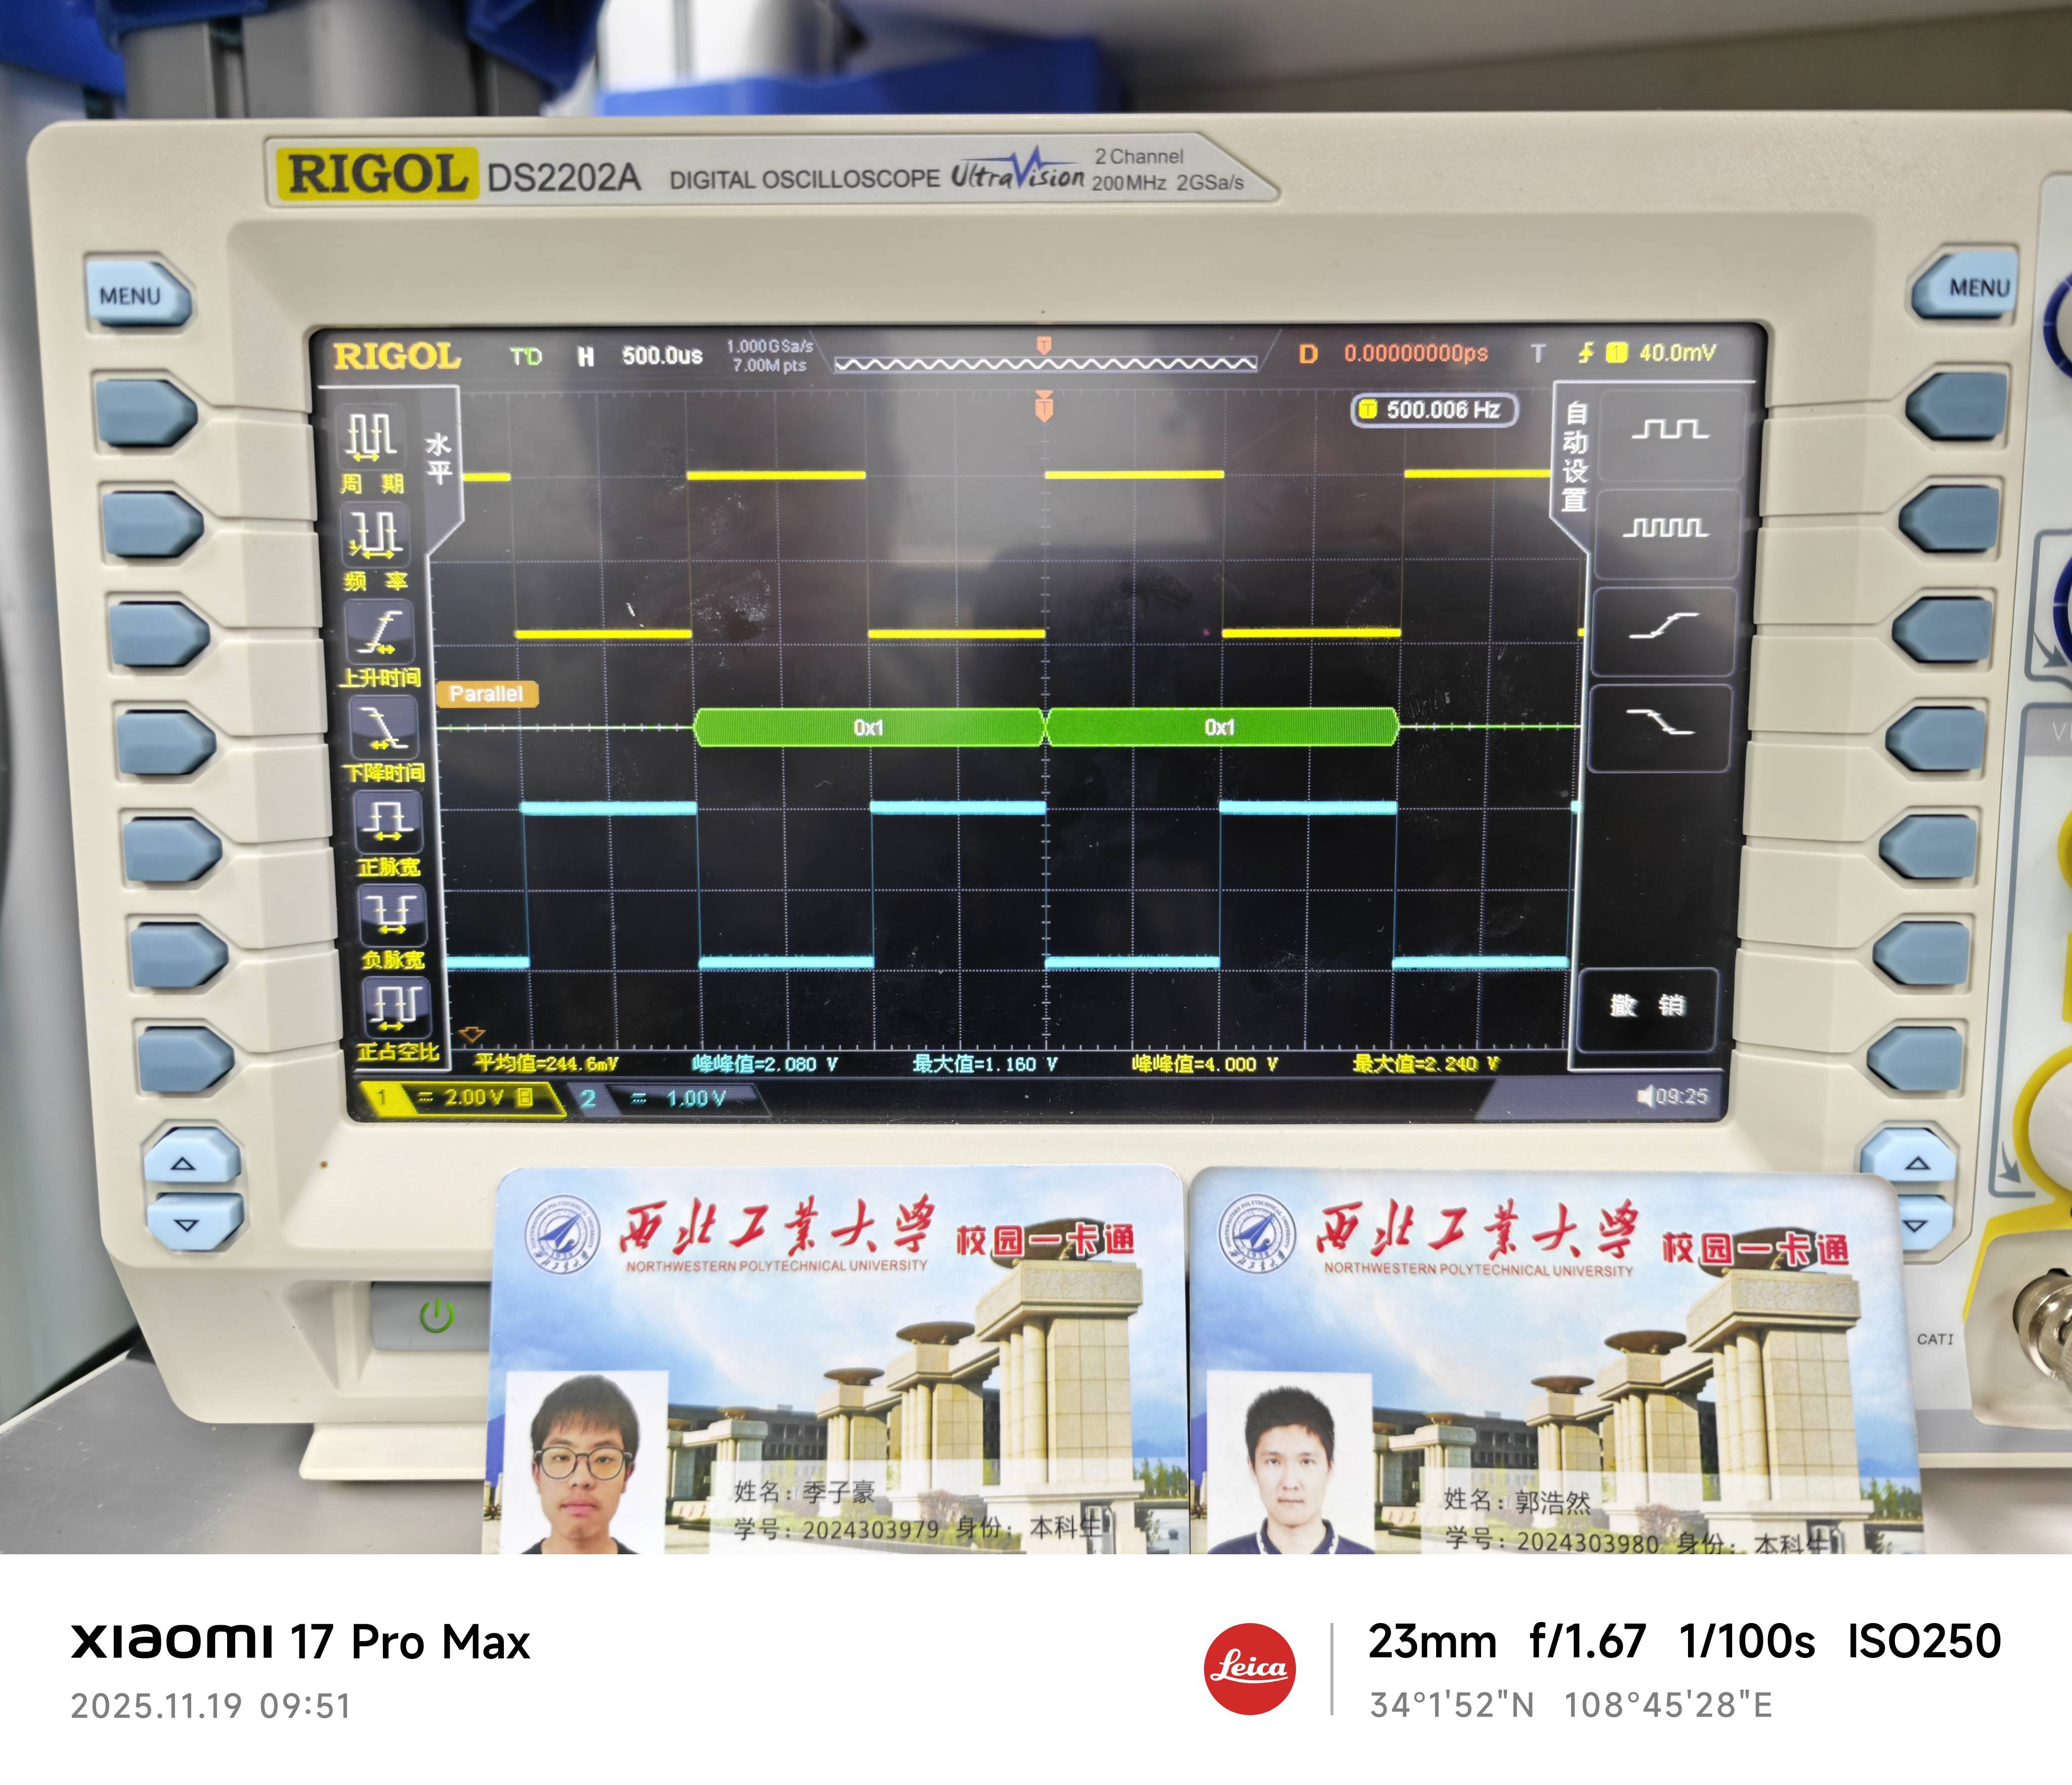
\includegraphics[width=\linewidth]{./3. convolution/figures/反相加法器.jpg}
        \caption{加法器混合输入波形}
        \label{fig:result-adder}
    \end{minipage}
\end{figure}

由表\ref{tab:adder-data}可知：输出电压大致等于两路输入电压之和取反相，验证了加法器的功能。

当输入一改为峰峰值为 \SI{2}{\volt}、频率为 \SI{500}{\hertz} 的方波时，波形如图\ref{fig:result-adder}所示。从图中可以看出，加法器实现了对输入方波的直流偏置与反相。

\subsubsection{比例放大器}
测得实验数据如表\ref{tab:prop-data}所示。对应的示波器波形如图\ref{fig:result-prop}所示。

\begin{table}[H]
    \centering
    \caption{比例放大器测试数据}
    \label{tab:prop-data}
    \begin{tabular}{ccccc}
        \toprule
        组号 & 电阻 & 输入电压 & 输入波形 & 输出电压 (\si{\volt}) \\
        \midrule
        1 & $R_1 = \SI{1}{\kilo\ohm},\; R_2 = \SI{5.1}{\kilo\ohm}$ & \SI{1.000}{\volt} & \SI{1}{\kilo\hertz} 正弦波 & \SI{4.560}{\volt} \\
        2 & $R_1 = \SI{1}{\kilo\ohm},\; R_2 = \SI{10}{\kilo\ohm}$  & \SI{980.0}{\milli\volt} & \SI{1}{\kilo\hertz} 正弦波 & \SI{9.200}{\volt} \\
        \bottomrule
    \end{tabular}
\end{table}


\begin{figure}[H]
    \centering
    \begin{subfigure}{0.48\textwidth}
        \centering
        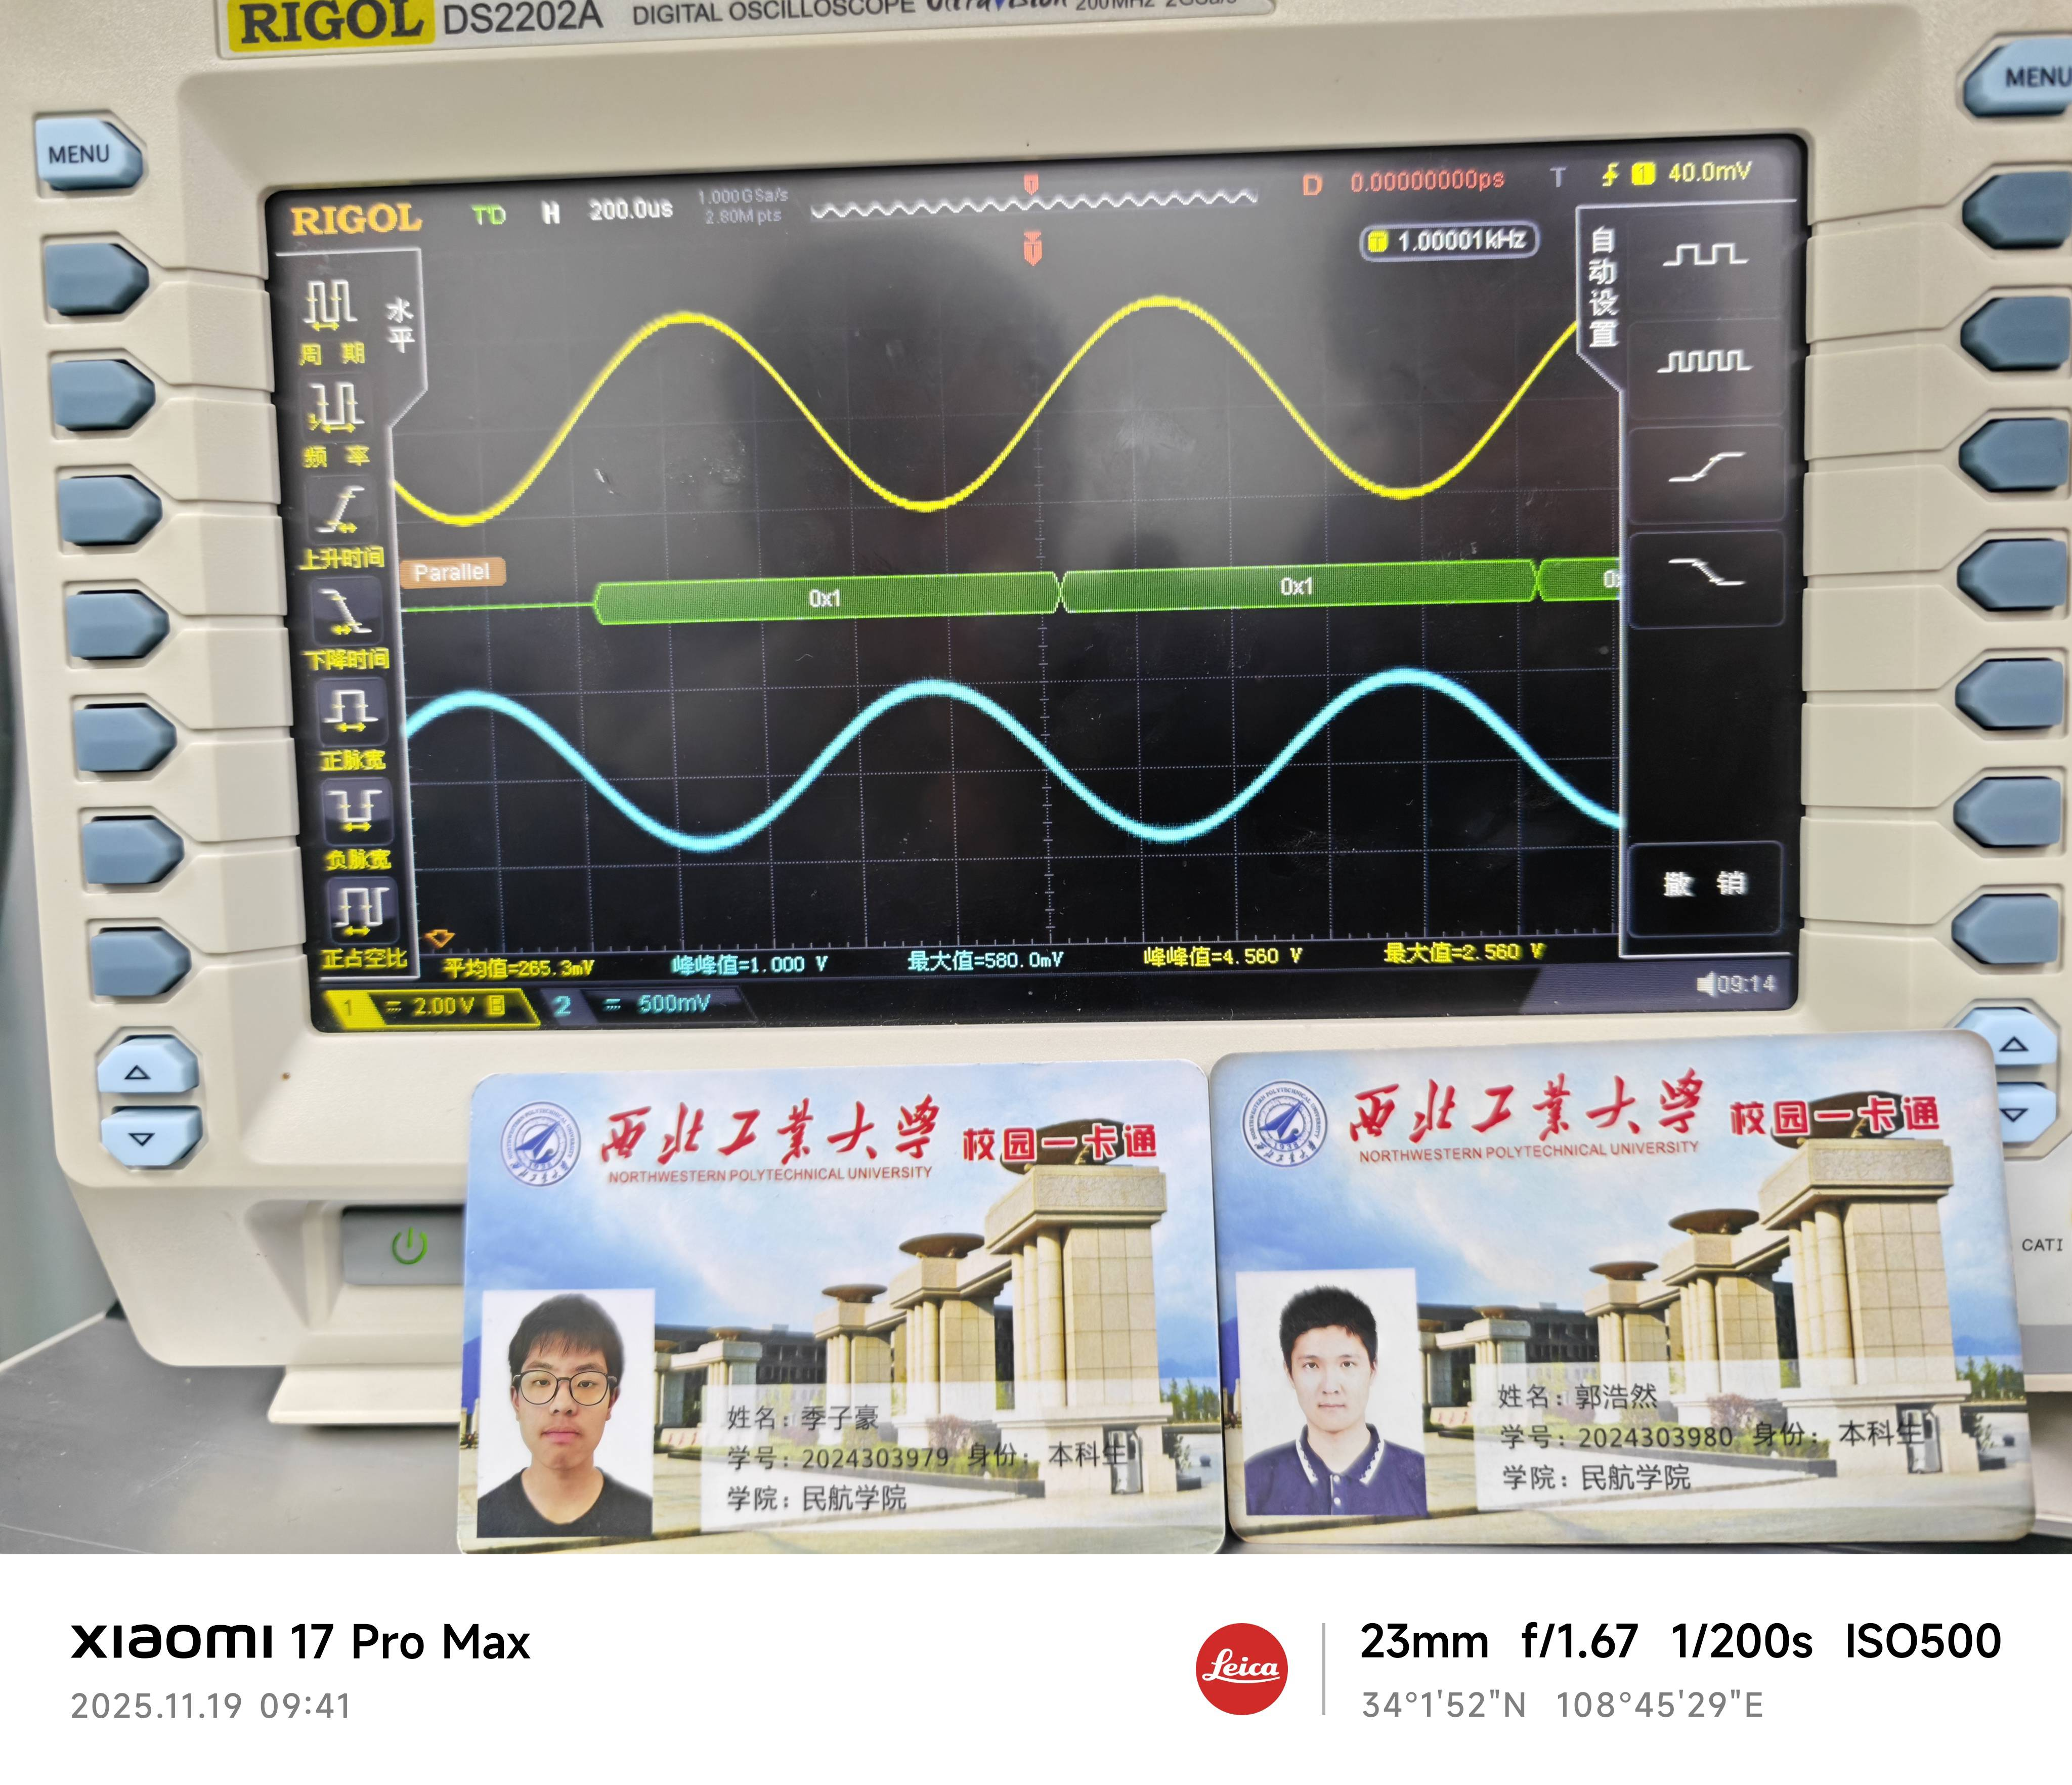
\includegraphics[width=\textwidth]{./3. convolution/figures/比例器2.jpg}
        \caption{第一组电阻 ($R_2 = \SI{5.1}{\kilo\ohm}$)}
    \end{subfigure}
    \hfill
    \begin{subfigure}{0.48\textwidth}
        \centering
        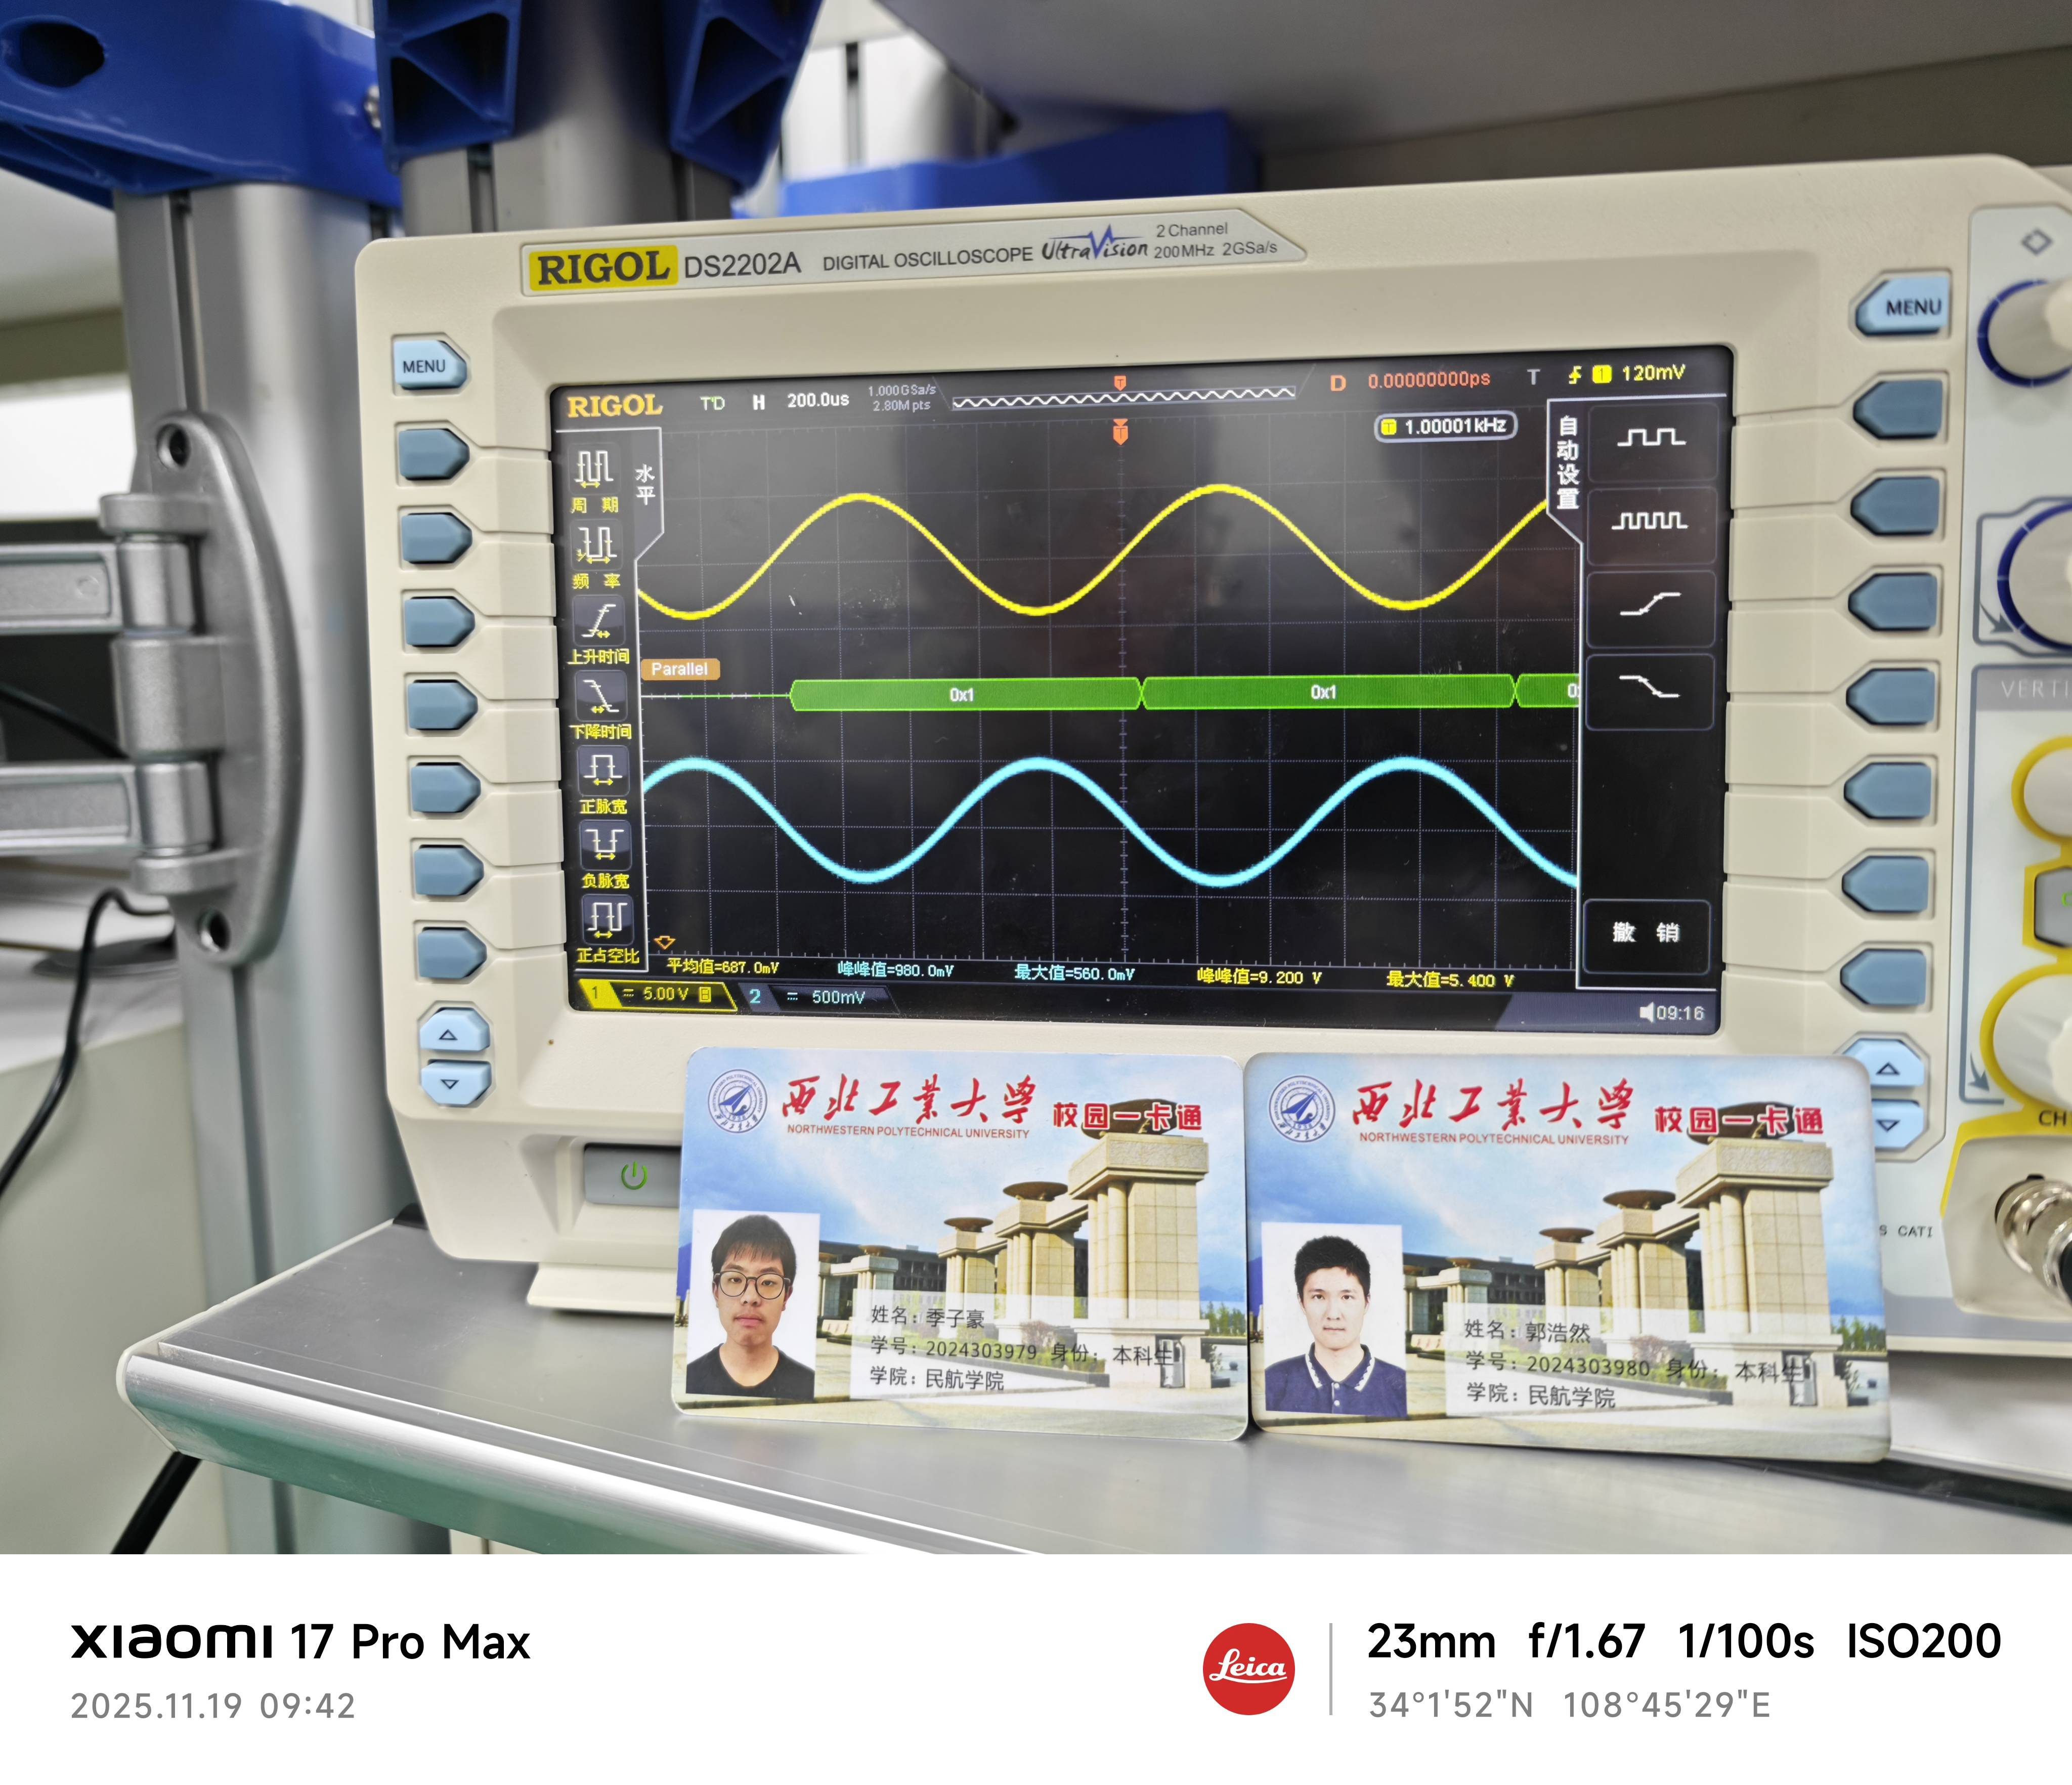
\includegraphics[width=\textwidth]{./3. convolution/figures/比例器1.jpg}
        \caption{第二组电阻 ($R_2 = \SI{10}{\kilo\ohm}$)}
    \end{subfigure}
    \caption{比例放大器输入输出波形}
    \label{fig:result-prop}
\end{figure}

\subsubsection{积分器}
输入信号为 $f = \SI{1}{\kilo\hertz}$ 的方波时，记录数据如表\ref{tab:int-data}所示。输入输出信号波形图如图\ref{fig:result-int}所示。

\begin{figure}[H]
    \centering
    % --- 左侧：表格 ---
    \begin{minipage}[c]{0.48\textwidth}
        \centering
        \captionof{table}{积分器测试数据}
        \label{tab:int-data}
        \small
        \begin{tabular}{ccc}
            \toprule
            电路参数 & \makecell[c]{输入 $V_{pp}$ \\ (\si{\volt})} & \makecell[c]{输出 $V_{pp}$ \\ (\si{\milli\volt})} \\
            \midrule
            \makecell[c]{$R_1 = \SI{1}{\kilo\ohm}$ \\ $R_2 = \SI{20}{\kilo\ohm}$} & 3.040 & 860.0 \\
            \bottomrule
        \end{tabular}
    \end{minipage}
    \hfill
    % --- 右侧：图片 ---
    \begin{minipage}[c]{0.48\textwidth}
        \centering
        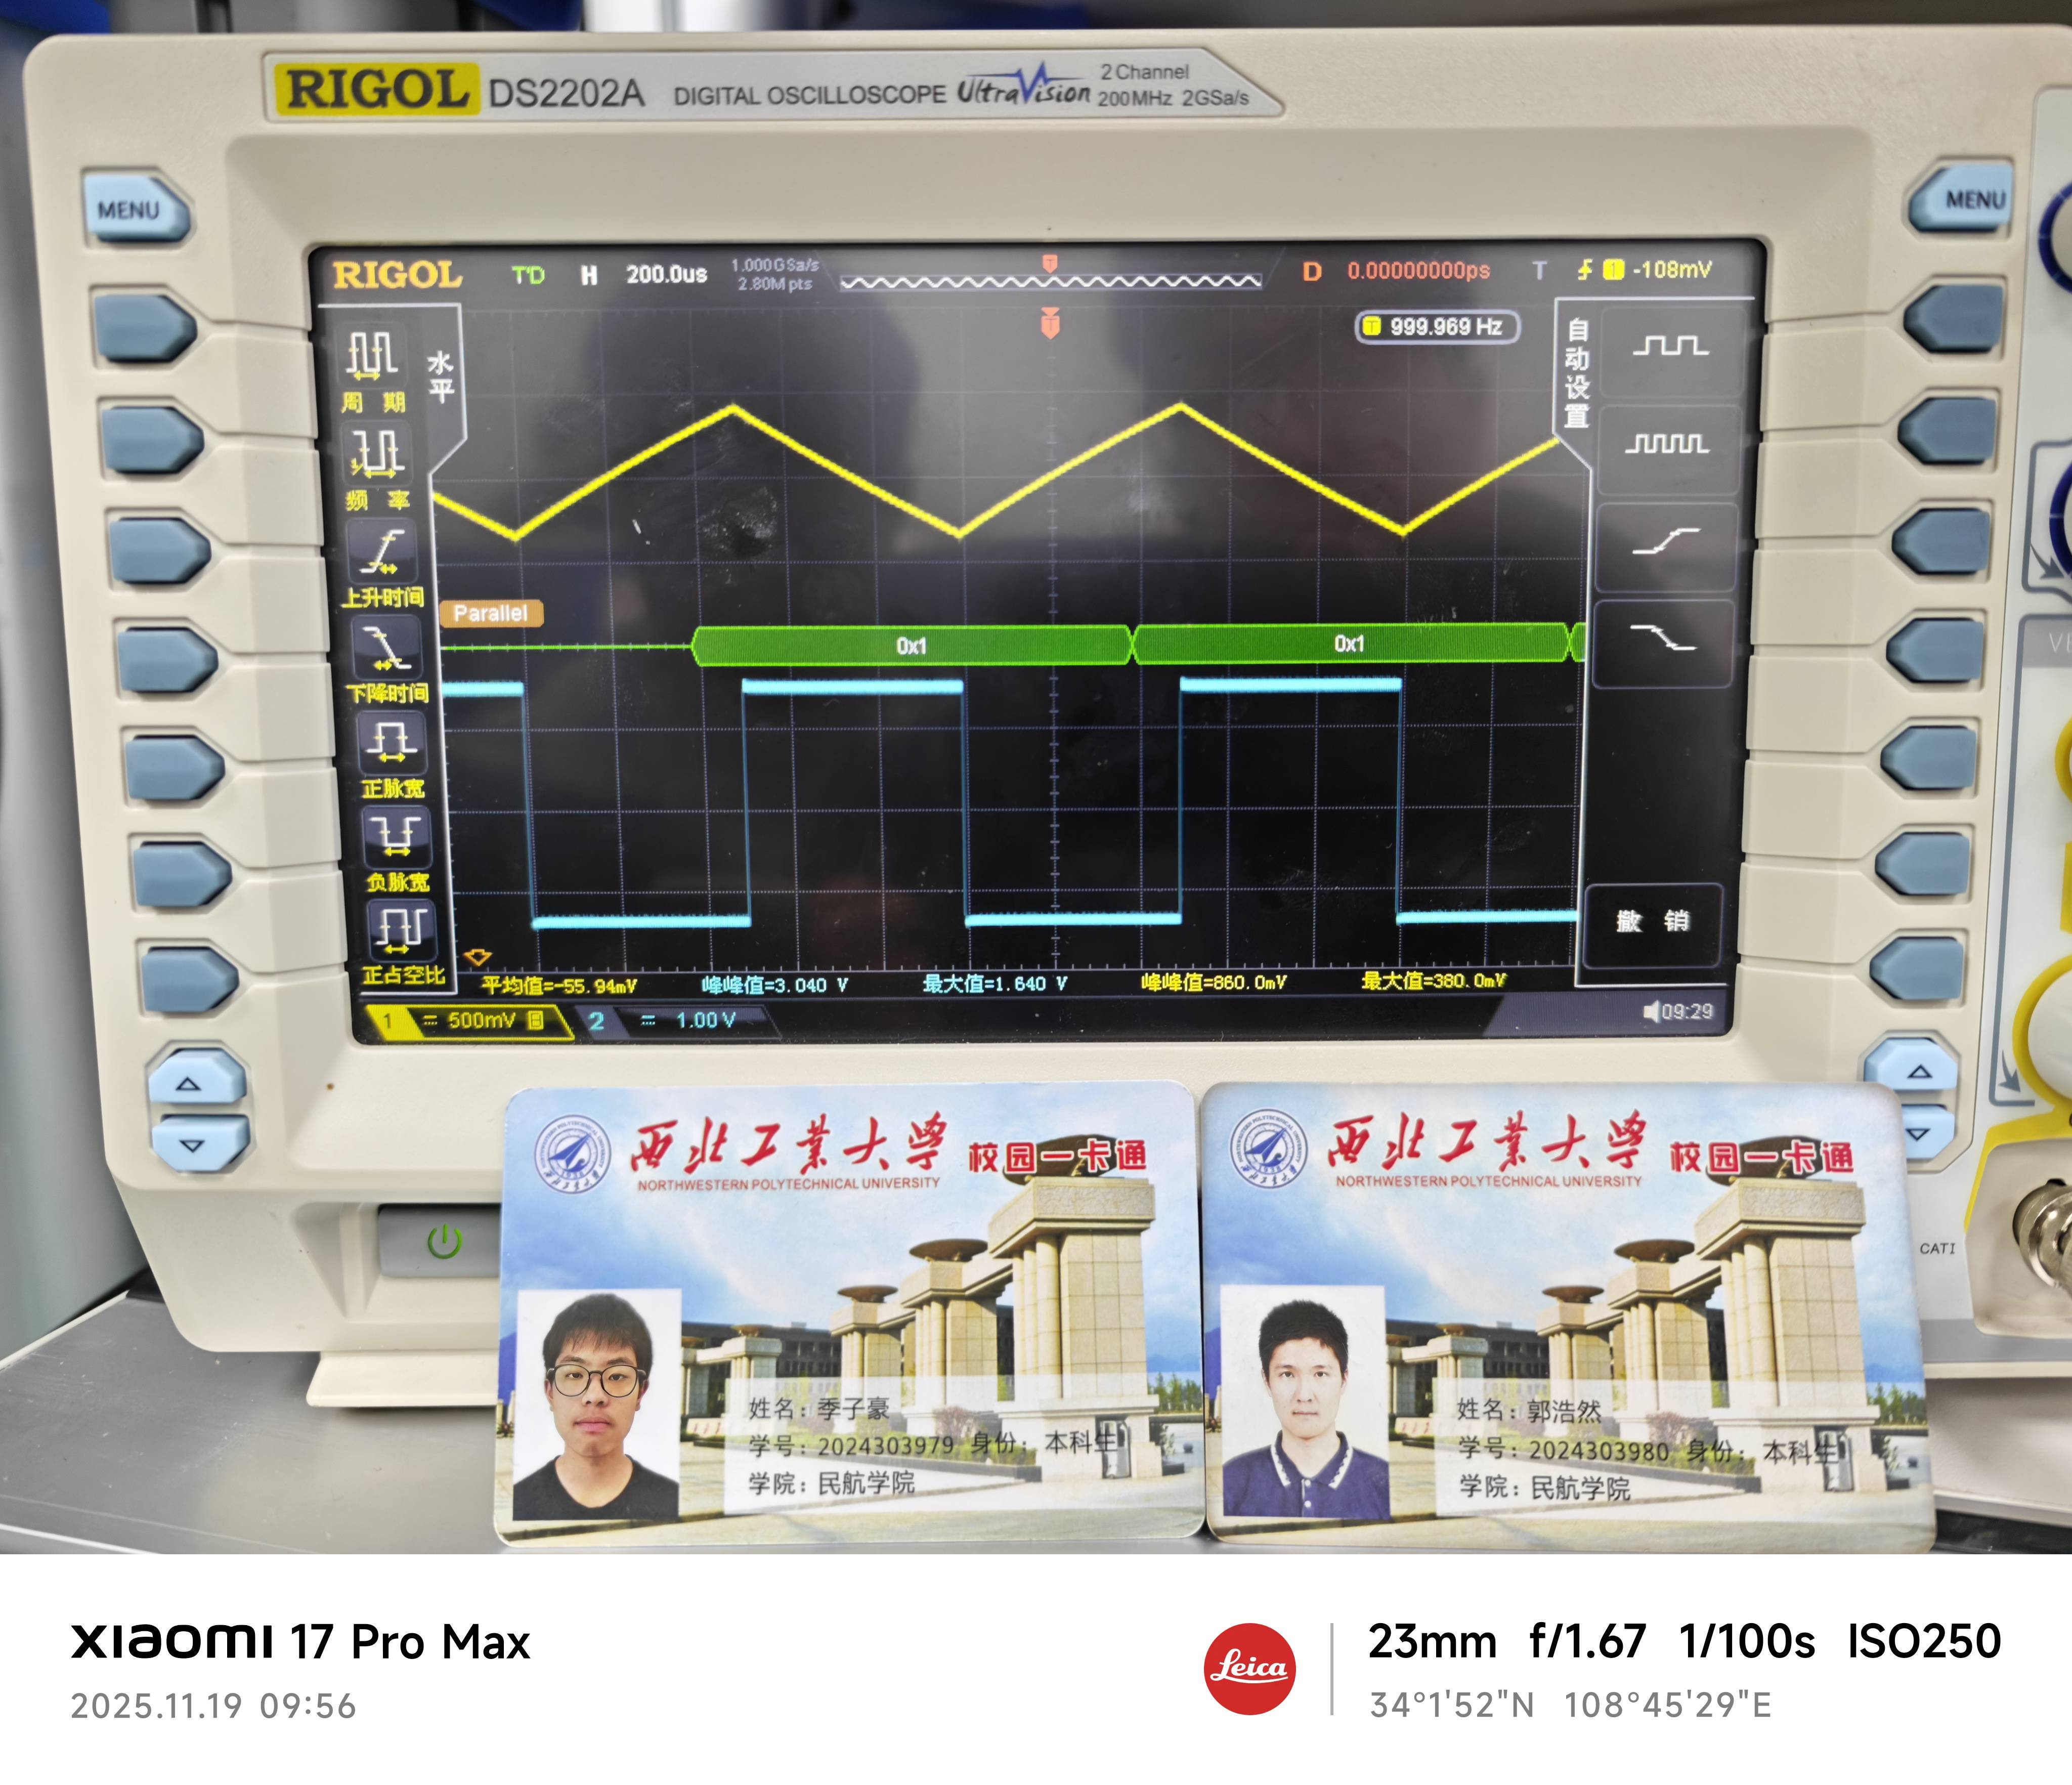
\includegraphics[width=\linewidth]{./3. convolution/figures/积分器.jpg}
        \caption{积分器输入输出波形（方波输入）}
        \label{fig:result-int}
    \end{minipage}
\end{figure}

\subsection{一阶模拟电路阶跃响应}
当输入为幅度 \SI{1}{\volt}、频率 \SI{1}{\kilo\hertz} 的方波（可近似为周期性阶跃信号）时，一阶RC模拟电路的输出电压波形如图\ref{fig:result-rc}所示，呈现出典型的RC电路充放电曲线。

\begin{figure}[H]
    \centering
    % --- 左侧：表格 ---
    \begin{minipage}[c]{0.48\textwidth}
        \centering
        \captionof{table}{一阶模拟电路阶跃响应参数记录}
        \label{tab:rc-params}
        \begin{tabular}{lcc}
            \toprule
            测量对象 & \makecell[c]{$V_{pp}$ \\ (\si{\volt})} & \makecell[c]{$f$ \\ (\si{\kilo\hertz})} \\
            \midrule
            输入信号 & 2.0 & 1.0 \\
            输出信号 & 1.63 & 1.0 \\
            \bottomrule
        \end{tabular}
    \end{minipage}
    \hfill
    % --- 右侧：图片 ---
    \begin{minipage}[c]{0.48\textwidth}
        \centering
        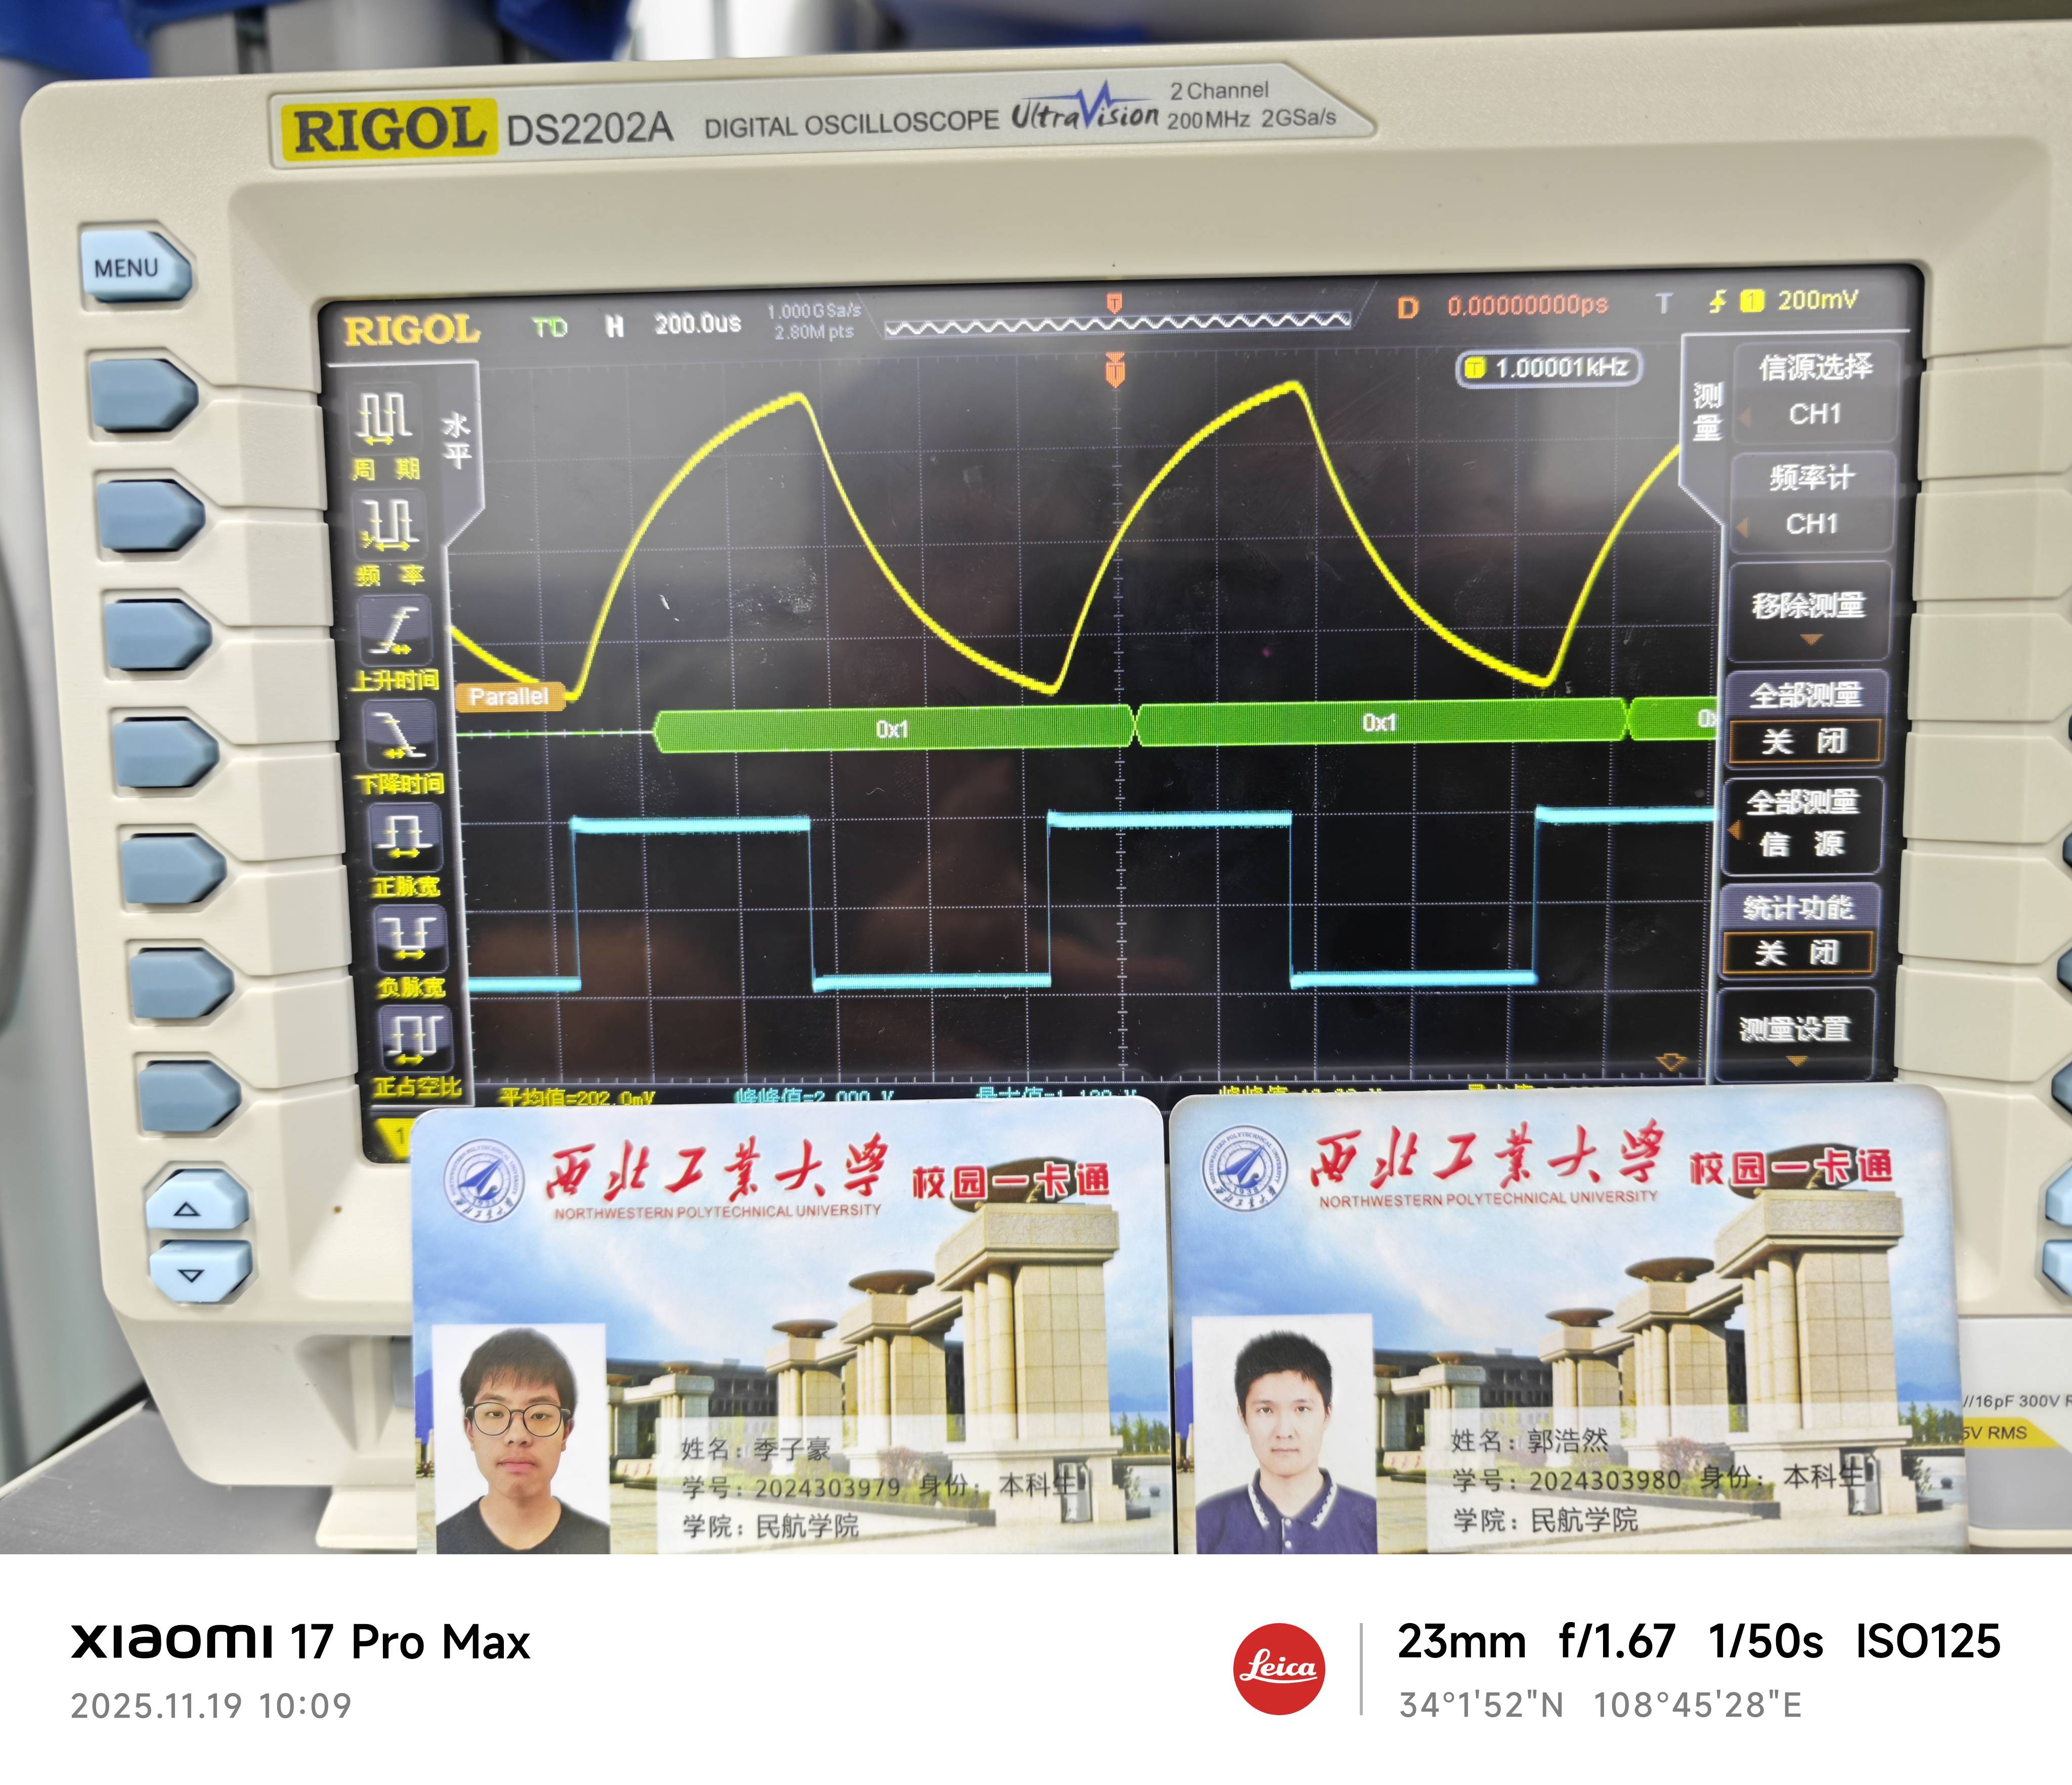
\includegraphics[width=\linewidth]{./3. convolution/figures/系统模拟.jpg}
        \caption{一阶RC电路模拟输出波形}
        \label{fig:result-rc}
    \end{minipage}
\end{figure}

\section{实验结论}
\begin{enumerate}
    \item 通过本次实验，我深入了解了比例放大器、加法器和积分器这三种基本运算单元的电路结构与实际运算功能。实验结果表明，加法器能够实现多路信号的代数和（反相），比例放大器的放大倍数由反馈电阻与输入电阻之比决定，积分器则能将方波输入转换为三角波输出，验证了其积分特性。
    
    \item 我掌握了使用基本运算单元搭建模拟电路的方法，并成功地运用加法器和积分器模拟了一阶RC电路的阶-跃响应。实验观测到的输出波形（如图\ref{fig:result-rc}所示）与理论上的指数充放电曲线高度吻合，直观地展示了通过模拟电路研究实际系统动态特性的可行性与有效性。
    
    \item 实验过程中也注意到，实际测量值与理论计算值存在微小的误差（例如比例放大器的放大倍数并非精确等于 $R_2/R_1$），这可能来源于运放器件的非理想特性、电阻元件的精度误差、导线电阻以及测量仪器的内部误差等因素。
\end{enumerate}

\section*{附录：MATLAB 信号仿真}
\addcontentsline{toc}{section}{附录: MATLAB 信号仿真}

本部分包含使用 MATLAB 进行信号卷积运算的仿真练习。

\subsection{课堂验收}
\begin{enumerate}
    \item 已知信号 $f(t) = e^{-t}u(t)$ 和 $h(t) = t^2e^{-2t}u(t)$，求 $y(t) = f(t) * h(t)$，结果如图\ref{fig:conv1}所示。
    \item 已知两信号 $f_1(t) = u(t) - u(t-1)$ 和 $f_2(t) = u(t+1) - u(t)$，求 $g_3(t) = f_1(t) * f_2(t)$，结果如图\ref{fig:conv2}所示。

    \begin{figure}[H]
        \centering
        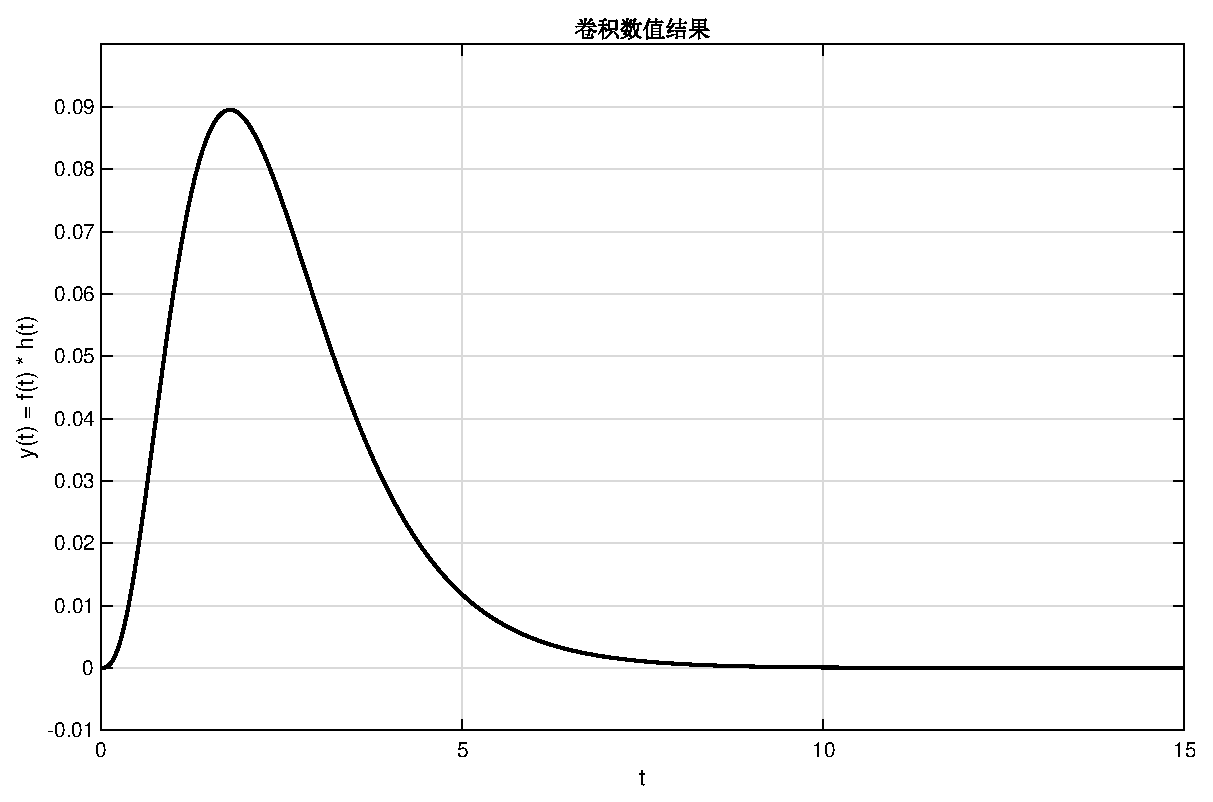
\includegraphics[width=0.6\textwidth]{./3. convolution/figures/conv1.eps}
        \caption{信号 $f(t)=e^{-t}u(t)$ 与 $h(t)=t^2e^{-2t}u(t)$ 的卷积结果}
        \label{fig:conv1}
    \end{figure}
    
    
    \begin{figure}[H]
        \centering
        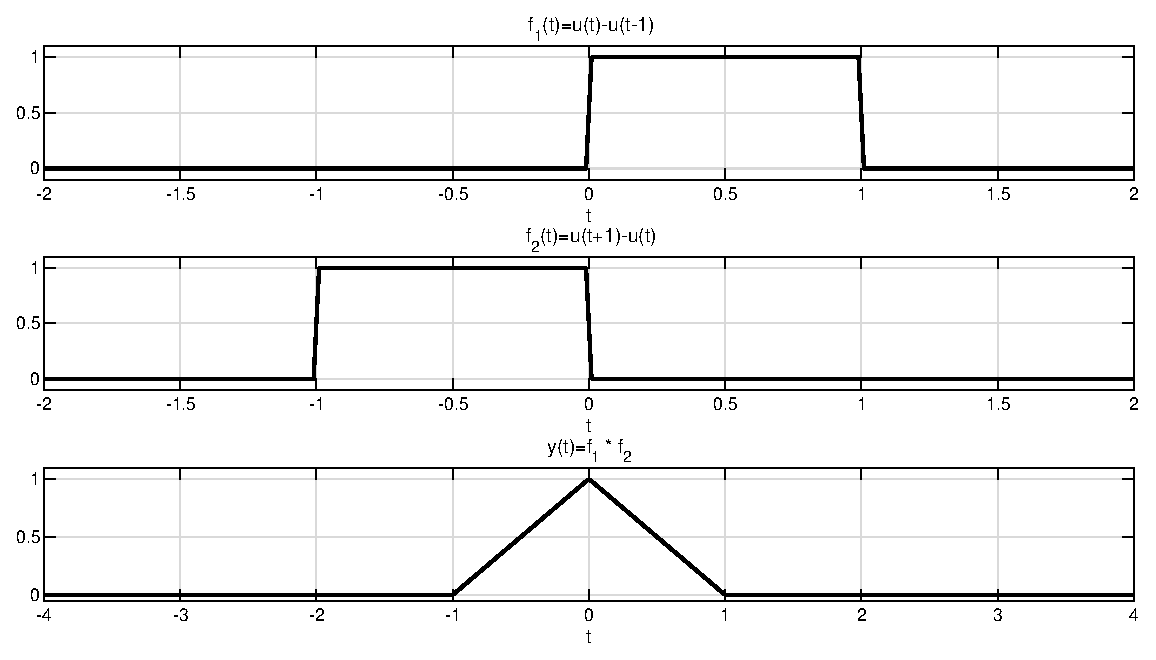
\includegraphics[width=0.6\textwidth]{./3. convolution/figures/conv2.eps}
        \caption{信号 $f_1(t)=u(t)-u(t-1)$ 与 $f_2(t)=u(t+1)-u(t)$ 的卷积结果}
        \label{fig:conv2}
    \end{figure}
\end{enumerate}

\subsection{作业练习}
\begin{enumerate}
    \item 已知 $f_1(t) = u(t) - u(t-1)$, $f_2(t) = u(t+1) - u(t)$，求 $g_1(t) = f_1(t) * f_1(t)$, $g_2(t) = f_2(t) * f_2(t)$, $g_3(t) = f_1(t) * f_2(t)$。其中 $g_3(t)$ 的波形如图\ref{fig:homework}(a)所示。
    \item 对$f_1(t) = u(t-1) - u(t-2)$ 和 $f_2(t) = u(t) + u(t-1) - u(t-2) - u(t-3)$ 进行卷积，结果如图\ref{fig:homework}(b)所示。
    \item 对 $f_1(t) = u(t+1) - u(t-1)$ 和 $f_2(t)$进行卷积，结果如图\ref{fig:homework}(c)所示。
    \item 已知 $f_1(t) = (t-1)[u(t-1) - u(t-3)]$ 和 $f_2(t) = u(t+1) - 2u(t-2)$，求卷积，结果如图\ref{fig:homework}(d)所示。
\end{enumerate}

\begin{figure}[H]
    \centering
    \begin{subfigure}[b]{0.48\textwidth}
        \centering
        
\includegraphics[width=\textwidth]{./3. convolution/figures/T1.eps}
        \caption{作业1结果}
    \end{subfigure}
    \hfill
    \begin{subfigure}[b]{0.48\textwidth}
        \centering
        
\includegraphics[width=\textwidth]{./3. convolution/figures/T2.eps}
        \caption{作业2结果}
    \end{subfigure}
    
    \vspace{1em} % 增加垂直间距
    
    \begin{subfigure}[b]{0.48\textwidth}
        \centering
        
\includegraphics[width=\textwidth]{./3. convolution/figures/T3.eps}
        \caption{作业3结果}
    \end{subfigure}
    \hfill
    \begin{subfigure}[b]{0.48\textwidth}
        \centering
        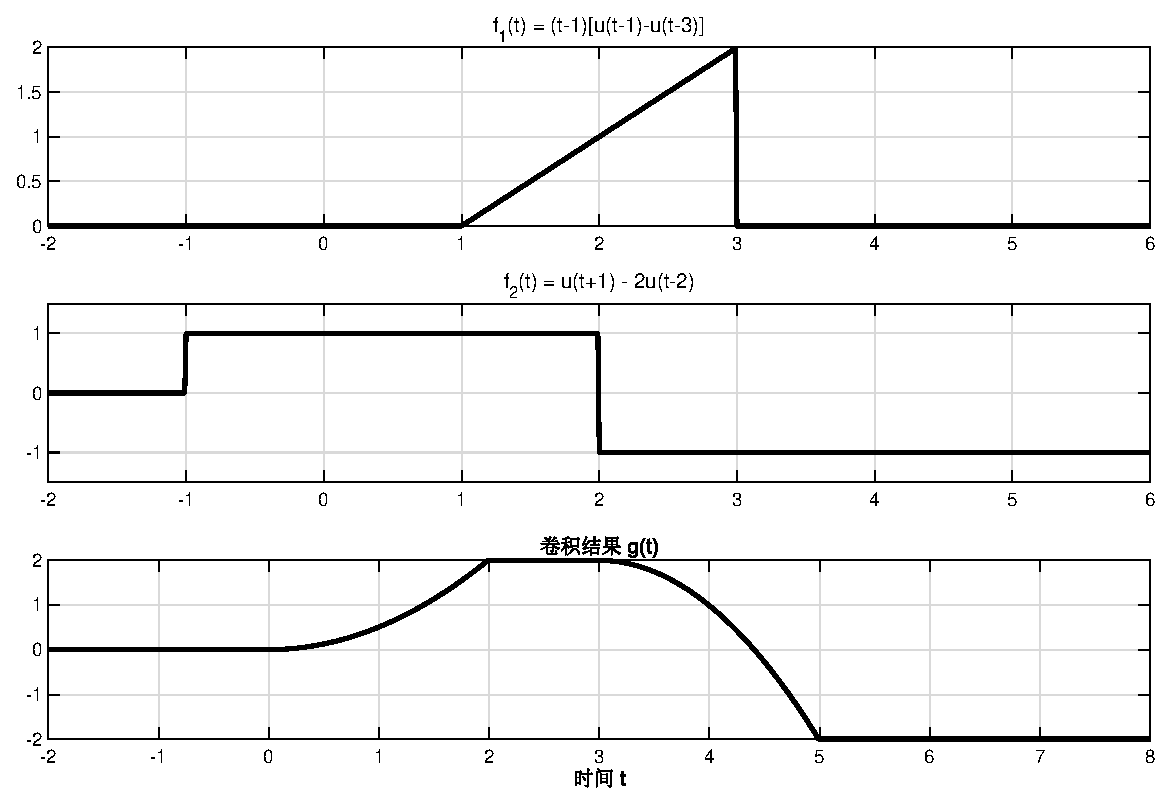
\includegraphics[width=\textwidth]{./3. convolution/figures/T4.eps}
        \caption{作业4结果}
    \end{subfigure}
    \caption{MATLAB 作业练习卷积结果}
    \label{fig:homework}
\end{figure}


% ===================================================================
% 第四章：有源、无源滤波器 (Origin: 4. frequency)
% ===================================================================
\chapter{有源、无源滤波器}

% ==========================================
% 第一部分：实验目的、器材与原理
% ==========================================

\section{实验目的}

\begin{enumerate}
    \item 熟悉滤波器的构成及其特性（包括有源、无源；低通、高通、带通、带阻）。
    \item 学会测量滤波器幅频特性的方法（点频法与扫频法）。
\end{enumerate}

\section{实验器材}

\begin{enumerate}
    \item 双踪示波器 \quad 1台
    \item 信号源及频率计模块 (S2) \quad 1块
    \item 抽样定理及滤波器模块 (S3) \quad 1块
\end{enumerate}

\section{实验原理}

滤波器是一种能使有用频率信号通过而同时抑制（或大为衰减）无用频率信号的电子装置。工程上常用它作信号处理、数据传送和抑制干扰等。

本实验主要讨论模拟滤波器。
\begin{itemize}
    \item \textbf{无源滤波器}：主要采用无源元件 $R$、$L$ 和 $C$ 组成。
    \item \textbf{有源滤波器}：由集成运放和 $R$、$C$ 组成。具有不用电感、体积小、重量轻等优点，且具有一定的电压放大和缓冲作用，但带宽受运放限制。
\end{itemize}

\subsection{基本概念及初步定义}

滤波电路的一般结构如图 \ref{fig:filter_structure} 所示。设输入信号为 $V_{i}(t)$，输出信号为 $V_{o}(t)$。

\begin{figure}[htbp]
    \centering
    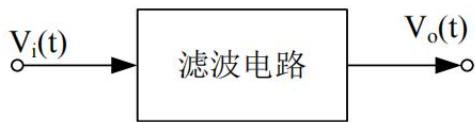
\includegraphics[width=0.6\textwidth]{./4. frequency/figures/原理图1.png} 
    \caption{滤波器电路的一般结构}
    \label{fig:filter_structure}
\end{figure}

假设滤波器是一个线性时不变网络，则在复频域内电压传递函数 $A(s)$ 定义为：
\begin{equation}
    A(s) = \frac{V_{o}(s)}{V_{i}(s)}
\end{equation}
对于实际频率（$s = j\omega$），则有：
\begin{equation}
    A(j\omega) = |A(j\omega)| e^{j\phi(\omega)}
\end{equation}
其中 $|A(j\omega)|$ 为幅频特性，$\phi(\omega)$ 为相频特性。

\subsection{各类滤波器的传输函数}

不同类型滤波器的理想传输函数及参数定义如表 \ref{tab:transfer_functions} 所示。

\begin{table}[htbp]
    \centering
    \caption{各类滤波器的传输函数及参数说明}
    \label{tab:transfer_functions}
    \renewcommand{\arraystretch}{2} % 增加行高，使公式更清晰
    \begin{tabular}{|c|c|l|}
        \hline
        \textbf{类型} & \textbf{传输函数} $A(s)$ & \multicolumn{1}{c|}{\textbf{备注}} \\
        \hline
        低通 & $\displaystyle \frac{A_V \omega_c^2}{s^2 + \frac{\omega_c}{Q}s + \omega_c^2}$ & \multirow{4}{*}{\makecell[l]{$A_V$ —— 电压增益 \\ $\omega_c$ —— 低、高通滤波器的截止角频率 \\ $\omega_o$ —— 带通、带阻滤波器的中心角频率 \\ $Q$ —— 品质因数 \\ $BW$ —— 带宽 \\ $Q \approx \frac{\omega_o}{BW}$ (当 $BW \ll \omega_o$ 时)}} \\
        \cline{1-2}
        高通 & $\displaystyle \frac{A_V s^2}{s^2 + \frac{\omega_c}{Q}s + \omega_c^2}$ & \\
        \cline{1-2}
        带通 & $\displaystyle \frac{A_V \frac{\omega_o}{Q}s}{s^2 + \frac{\omega_o}{Q}s + \omega_o^2}$ & \\
        \cline{1-2}
        带阻 & $\displaystyle \frac{A_V (s^2 + \omega_o^2)}{s^2 + \frac{\omega_o}{Q}s + \omega_o^2}$ & \\
        \hline
    \end{tabular}
\end{table}

\subsection{滤波电路的分类与幅频响应}

根据幅频响应，滤波电路通常分为以下四类（如图 \ref{fig:freq_response} 所示）：

\begin{enumerate}
    \item \textbf{低通 (LPF)}：通带 $0 \sim \omega_H$，截止频率 $BW = \omega_H$。
    \item \textbf{高通 (HPF)}：通带 $\omega > \omega_L$。
    \item \textbf{带通 (BPF)}：通带 $\omega_L \sim \omega_H$，带宽 $BW = \omega_H - \omega_L$。
    \item \textbf{带阻 (BEF)}：阻带 $\omega_H \sim \omega_L$，中心频率 $\omega_o$。
\end{enumerate}

\begin{figure}[htbp]
    \centering
    \begin{subfigure}{0.35\textwidth}
        \centering
        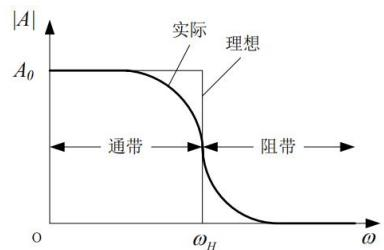
\includegraphics[width=\textwidth]{./4. frequency/figures/lpf.png}
        \caption{低通滤波器 LPF}
    \end{subfigure}
    % \hfill
    \begin{subfigure}{0.35\textwidth}
        \centering
        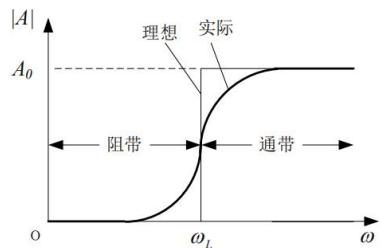
\includegraphics[width=\textwidth]{./4. frequency/figures/hpf.png}
        \caption{高通滤波器 HPF}
    \end{subfigure}

    \vspace{0.5cm}

    \begin{subfigure}{0.35\textwidth}
        \centering
        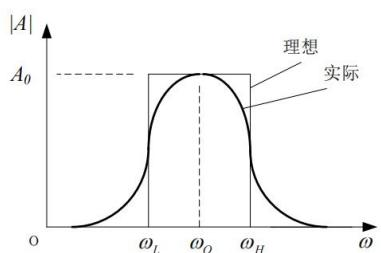
\includegraphics[width=\textwidth]{./4. frequency/figures/bpf.png}
        \caption{带通滤波器 BPF}
    \end{subfigure}
    % \hfill
    \begin{subfigure}{0.35\textwidth}
        \centering
        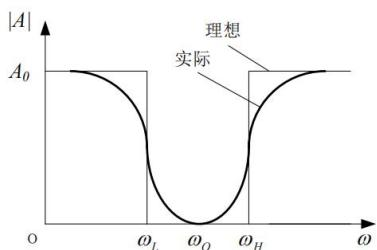
\includegraphics[width=\textwidth]{./4. frequency/figures/bef.png}
        \caption{带阻滤波器 BEF}
    \end{subfigure}

    \caption{各种滤波电路的幅频响应}
    \label{fig:freq_response}
\end{figure}

\section{实验步骤}

实验中信号源的输入信号均为 $4\,\mathrm{V}$ 左右的正弦波。

\textbf{设置模块}：按下波形切换 S4，使“SIN”指示灯亮，调节“模拟输出幅度调节”旋钮，使信号幅度为 $4\,\mathrm{V}$。

% ---------------------------------------------------------
% 任务一
% ---------------------------------------------------------
\subsection{任务一：测量低通滤波器的频响特性}

\subsubsection{逐点测量法（点频法）}

\begin{enumerate}
    \item 模块关电，连接模块 S2 中模拟信号输出端 P2 与模块 S3 中 P1（低通无源），保持输入信号幅度为 $4\,\mathrm{V}$ 不变。
    
    \begin{figure}[htbp]
        \centering
        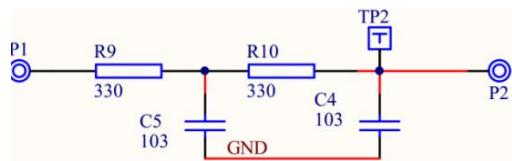
\includegraphics[width=0.6\textwidth]{./4. frequency/figures/原理图_无源低通.png} 
        \caption{无源低通滤波器接线示意}
    \end{figure}

    \item 模块开电，逐渐改变输入信号频率，并用示波器观测 TP2 处信号波形的峰峰值。
    \item 将数据记录（后续填入数据分析章节的表中）。
    \item 连接模块 S2 中模拟信号输出端 P2 与模块 S3 中 P5（低通有源）。
    \item 逐渐改变输入信号频率，并用示波器观测 TP6 处信号波形的峰峰值。
    \item 将数据记录。
    
    \begin{figure}[htbp]
        \centering
        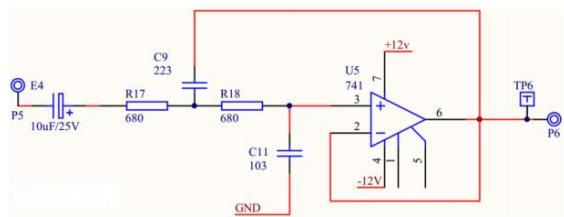
\includegraphics[width=0.6\textwidth]{./4. frequency/figures/原理图_有源低通.png}
        \caption{有源低通滤波器接线示意}
    \end{figure}
\end{enumerate}

\subsubsection{扫频法测量}

\textbf{原理}：S2 模块产生扫频信号，当它经过滤波器后，对比分析输入和输出的信号频率，就可以知道滤波器的特性。

\textbf{步骤}：
\begin{enumerate}
    \item 将扫频范围设置为 $100\,\mathrm{Hz} \sim 35\,\mathrm{kHz}$。
    \item 把示波器连接到信号源上输出 P2 处（示波器调为直流测试档），此时点 P2 输出扫频信号。
    \item 模块关电，分别把 S2 中 P2 输出的扫频信号输入到模块 S3 低通滤波器的输入端 P1（无源）或 P5（有源）。
    \item 模块开电，示波器另一通道接输出，拍照记录此时示波器上的输入输出信号。
\end{enumerate}

% ---------------------------------------------------------
% 任务二
% ---------------------------------------------------------
\subsection{任务二：测量高通滤波器的频响特性}

\subsubsection{逐点测量法（点频法）}

\begin{enumerate}
    \item 模块关电，保持信号源输出的正弦信号幅度不变，连接模块 S2 中模拟信号源部分 P2 与模块 S3 中模拟滤波器中的 P3（高通无源）端口。
    
    \begin{figure}[htbp]
        \centering
        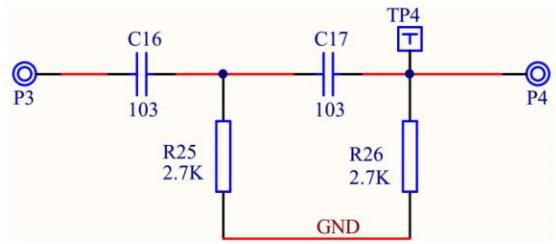
\includegraphics[width=0.6\textwidth]{./4. frequency/figures/原理图_无源高通.png}
        \caption{高通无源滤波器接线示意}
    \end{figure}

    \item 模块开电，逐渐改变输入信号频率，并用示波器观测 TP4 处信号波形的峰峰值。
    \item 将数据记录。
    \item 模块关电，连接模块 S3 中模拟信号输出端 P2 与模块 S3 中模拟滤波器中的 P7（高通有源）。
    
    \begin{figure}[htbp]
        \centering
        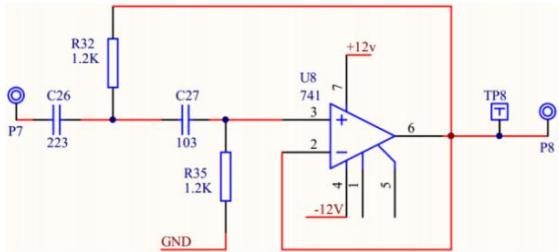
\includegraphics[width=0.6\textwidth]{./4. frequency/figures/原理图_有源高通.png}
        \caption{高通有源滤波器接线示意}
    \end{figure}

    \item 模块开电，逐渐改变输入信号频率，并用示波器观测 TP8 处信号波形的峰峰值。
    \item 将数据记录。
\end{enumerate}

\subsubsection{扫频法测量}

将扫频范围设置为 $100\,\mathrm{Hz} \sim 35\,\mathrm{kHz}$，把示波器连接到信号源上输出 P2 处（示波器调为直流测试档），此时点 P2 输出扫频信号。模块关电，把扫频信号输入到高通滤波器的输入端，模块开电，拍照记录此时的输入输出信号。

% ---------------------------------------------------------
% 任务三
% ---------------------------------------------------------
\subsection{任务三：测量带通滤波器的频响特性}

\subsubsection{逐点测量法}

\begin{enumerate}
    \item 模块关电，保持信号源输出的正弦信号幅度不变，连接模块 S2 中 P2 与模块 S3 中模拟滤波器中的 P9 相连（带通无源）。
    
    \begin{figure}[htbp]
        \centering
        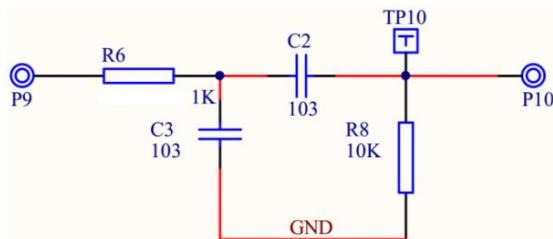
\includegraphics[width=0.6\textwidth]{./4. frequency/figures/原理图_无源带通.png}
        \caption{带通无源滤波器接线示意}
    \end{figure}

    \item 模块开电，逐渐改变输入信号频率，并用示波器观测 TP10 处信号波形的峰峰值。
    \item 将数据记录。
    \item 模块关电，保持信号源输出的正弦波幅度为 $4\,\mathrm{V}$ 不变，连接模块 S2 中 P2 与模块 S3 中模拟滤波器中的 P13（带通有源）。
    \item 模块开电，逐渐改变输入信号频率，并用示波器观测 TP14 处信号波形的峰峰值。
    \item 将数据记录。
\end{enumerate}

\subsubsection{扫频法测量}

将扫频范围设置为 $100\,\mathrm{Hz} \sim 35\,\mathrm{kHz}$，把示波器连接到信号源上输出 P2 处（示波器调为直流测试档），此时点 P2 输出扫频信号。把扫频信号输入到带通滤波器的输入端，拍照记录此时的输入输出信号。

% ---------------------------------------------------------
% 任务四
% ---------------------------------------------------------
\subsection{任务四：测量带阻滤波器的频响特性}

\subsubsection{逐点测量法}

\begin{enumerate}
    \item 模块关电，保持信号源输出的正弦信号幅度不变，连接模块 S2 中 P2 与模块 S3 中模拟滤波器中的 P11（带阻无源）。
    \item 模块开电，逐渐改变输入信号频率，并用示波器观测 TP12 处信号波形的峰峰值。
    \item 将数据记录。
    
    \begin{figure}[htbp]
        \centering
        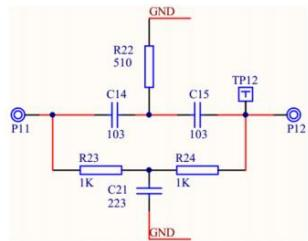
\includegraphics[width=0.6\textwidth]{./4. frequency/figures/原理图_无源带阻.png}
        \caption{带阻无源滤波器接线示意}
    \end{figure}

    \item 模块关电，保持信号源输出的正弦信号幅度 $4\,\mathrm{V}$ 不变，连接模块 S2 中 P2 与模块 S3 中模拟滤波器中的 P15（带阻有源）。
    
    \begin{figure}[htbp]
        \centering
        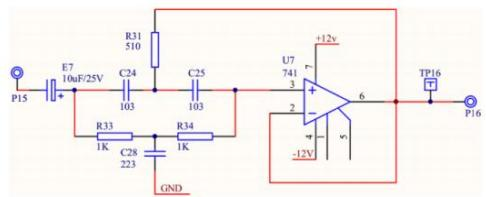
\includegraphics[width=0.6\textwidth]{./4. frequency/figures/原理图_有源带阻.png}
        \caption{带阻有源滤波器接线示意}
    \end{figure}

    \item 模块开电，逐渐改变输入信号频率，并用示波器观测 TP16 处信号波形的峰峰值。
    \item 将数据记录。
\end{enumerate}

\subsubsection{扫频法测量}

将扫频范围设置为 $100\,\mathrm{Hz} \sim 80\,\mathrm{kHz}$，把示波器连接到信号源上输出 P2 处（示波器调为直流测试档），此时点 P2 输出扫频信号。模块关电，把扫频信号输入到带阻滤波器的输入端，模块开电，对比观察输入输出信号。



\section{实验记录与数据分析}

% 定义通用表格命令，包含 resizebox 以防止表格超宽
\newcommand{\mygridtable}[2]{
    \begin{table}[H]
        \centering
        \renewcommand{\arraystretch}{1.4} % 增加行高
        \setlength{\tabcolsep}{3pt}       % 减小列间距
        % 使用 resizebox 强制表格适应文本宽度，避免拆分
        \resizebox{\textwidth}{!}{
            #1
        }
        \caption{#2}
    \end{table}
}

% ---------------------------------------------------------
% 任务一：低通滤波器
% ---------------------------------------------------------
\subsection{任务一：测量低通滤波器的频响特性}

\subsubsection{逐点测量法数据}

\textbf{1. 无源低通滤波器}

\mygridtable{
    \begin{tabular}{|c|c|c|c|c|c|c|c|c|c|c|c|}
        \hline
        $V_i$ (V) & 4 & 4 & 4 & 4 & 4 & 4 & 4 & 4 & 4 & 4 & 4 \\
        \hline
        $f$ (Hz) & 100 & 1k & 5k & 10k & 15k & \textbf{18.5k} & 20k & 25k & 30k & 50k & 100k \\
        \hline
        $V_o$ (V) & 3.84 & 3.84 & 3.84 & 3.44 & 3.04 & \textbf{2.80} & 2.72 & 2.40 & 2.08 & 1.36 & 0.72 \\
        \hline
        \multicolumn{12}{|l|}{\textbf{测量结论：} 当 $V_o \approx 0.707 V_i \approx 2.828\,\mathrm{V}$ 时，测得截止频率 $f_H = 18.5\,\mathrm{kHz}$} \\
        \hline
    \end{tabular}
}{低通无源滤波器逐点测量数据}

\textbf{2. 有源低通滤波器}

\mygridtable{
    \begin{tabular}{|c|c|c|c|c|c|c|c|c|c|c|c|}
        \hline
        $V_i$ (V) & 4 & 4 & 4 & 4 & 4 & 4 & 4 & 4 & 4 & 4 & 4 \\
        \hline
        $f$ (Hz) & 100 & 1k & 5k & 10k & \textbf{16.7k} & 17k & 20k & 25k & 30k & 50k & 100k \\
        \hline
        $V_o$ (V) & 3.84 & 3.84 & 3.84 & 3.68 & \textbf{2.80} & 2.72 & 2.24 & 1.60 & 1.28 & 0.56 & 0.24 \\
        \hline
        \multicolumn{12}{|l|}{\textbf{测量结论：} 当 $V_o \approx 0.707 V_i \approx 2.828\,\mathrm{V}$ 时，测得截止频率 $f_H = 16.7\,\mathrm{kHz}$} \\
        \hline
    \end{tabular}
}{低通有源滤波器逐点测量数据}

\subsubsection{幅频特性曲线与扫频测试}

\begin{figure}[H]
    \centering
    \begin{subfigure}[b]{0.8\textwidth}
        \centering
        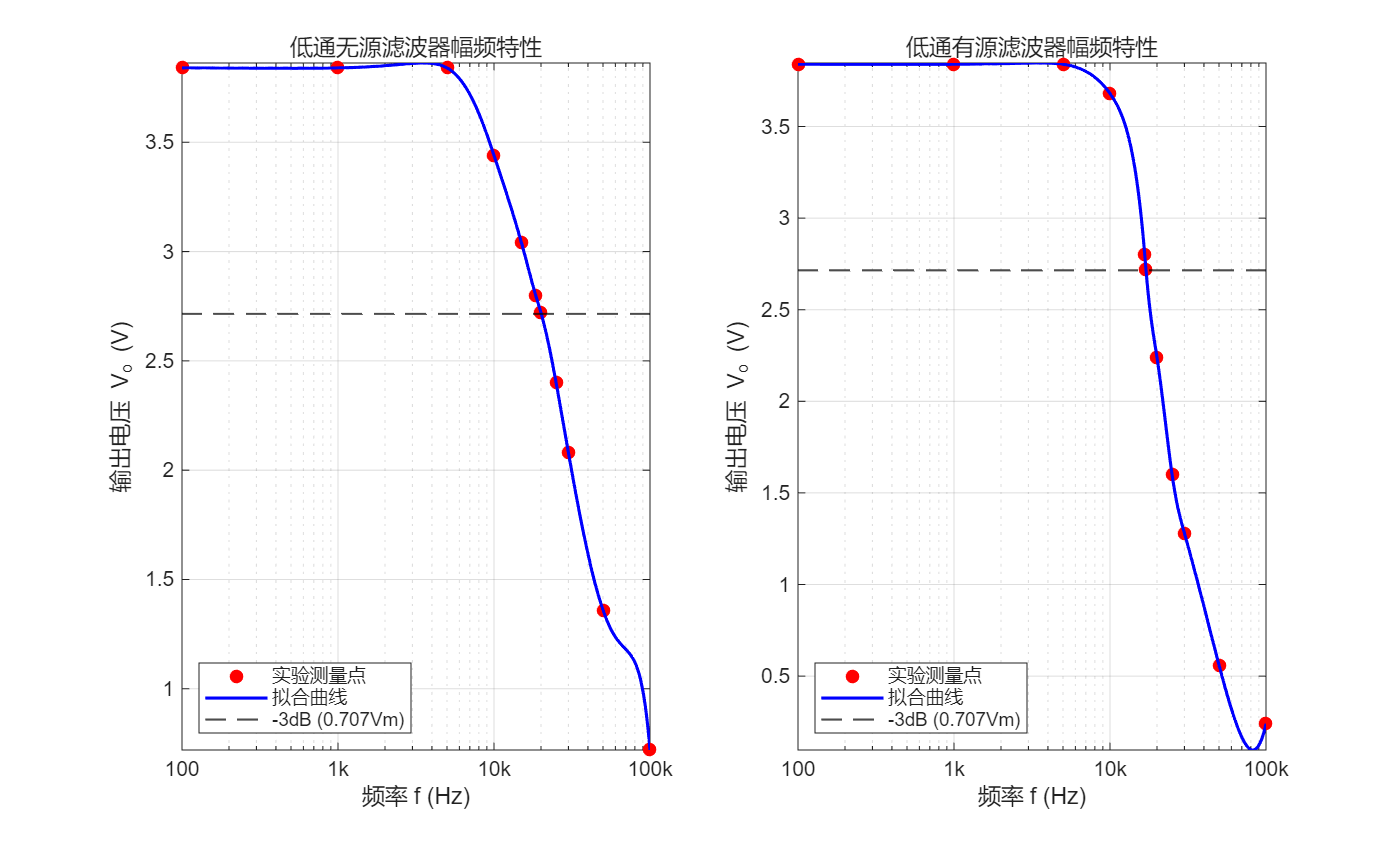
\includegraphics[width=\textwidth]{./4. frequency/figures/低通.png}
        \caption{低通滤波器幅频特性曲线 (MATLAB)}
    \end{subfigure}
    
    \vspace{1em}
    
    \begin{subfigure}[b]{0.45\textwidth}
        \centering
        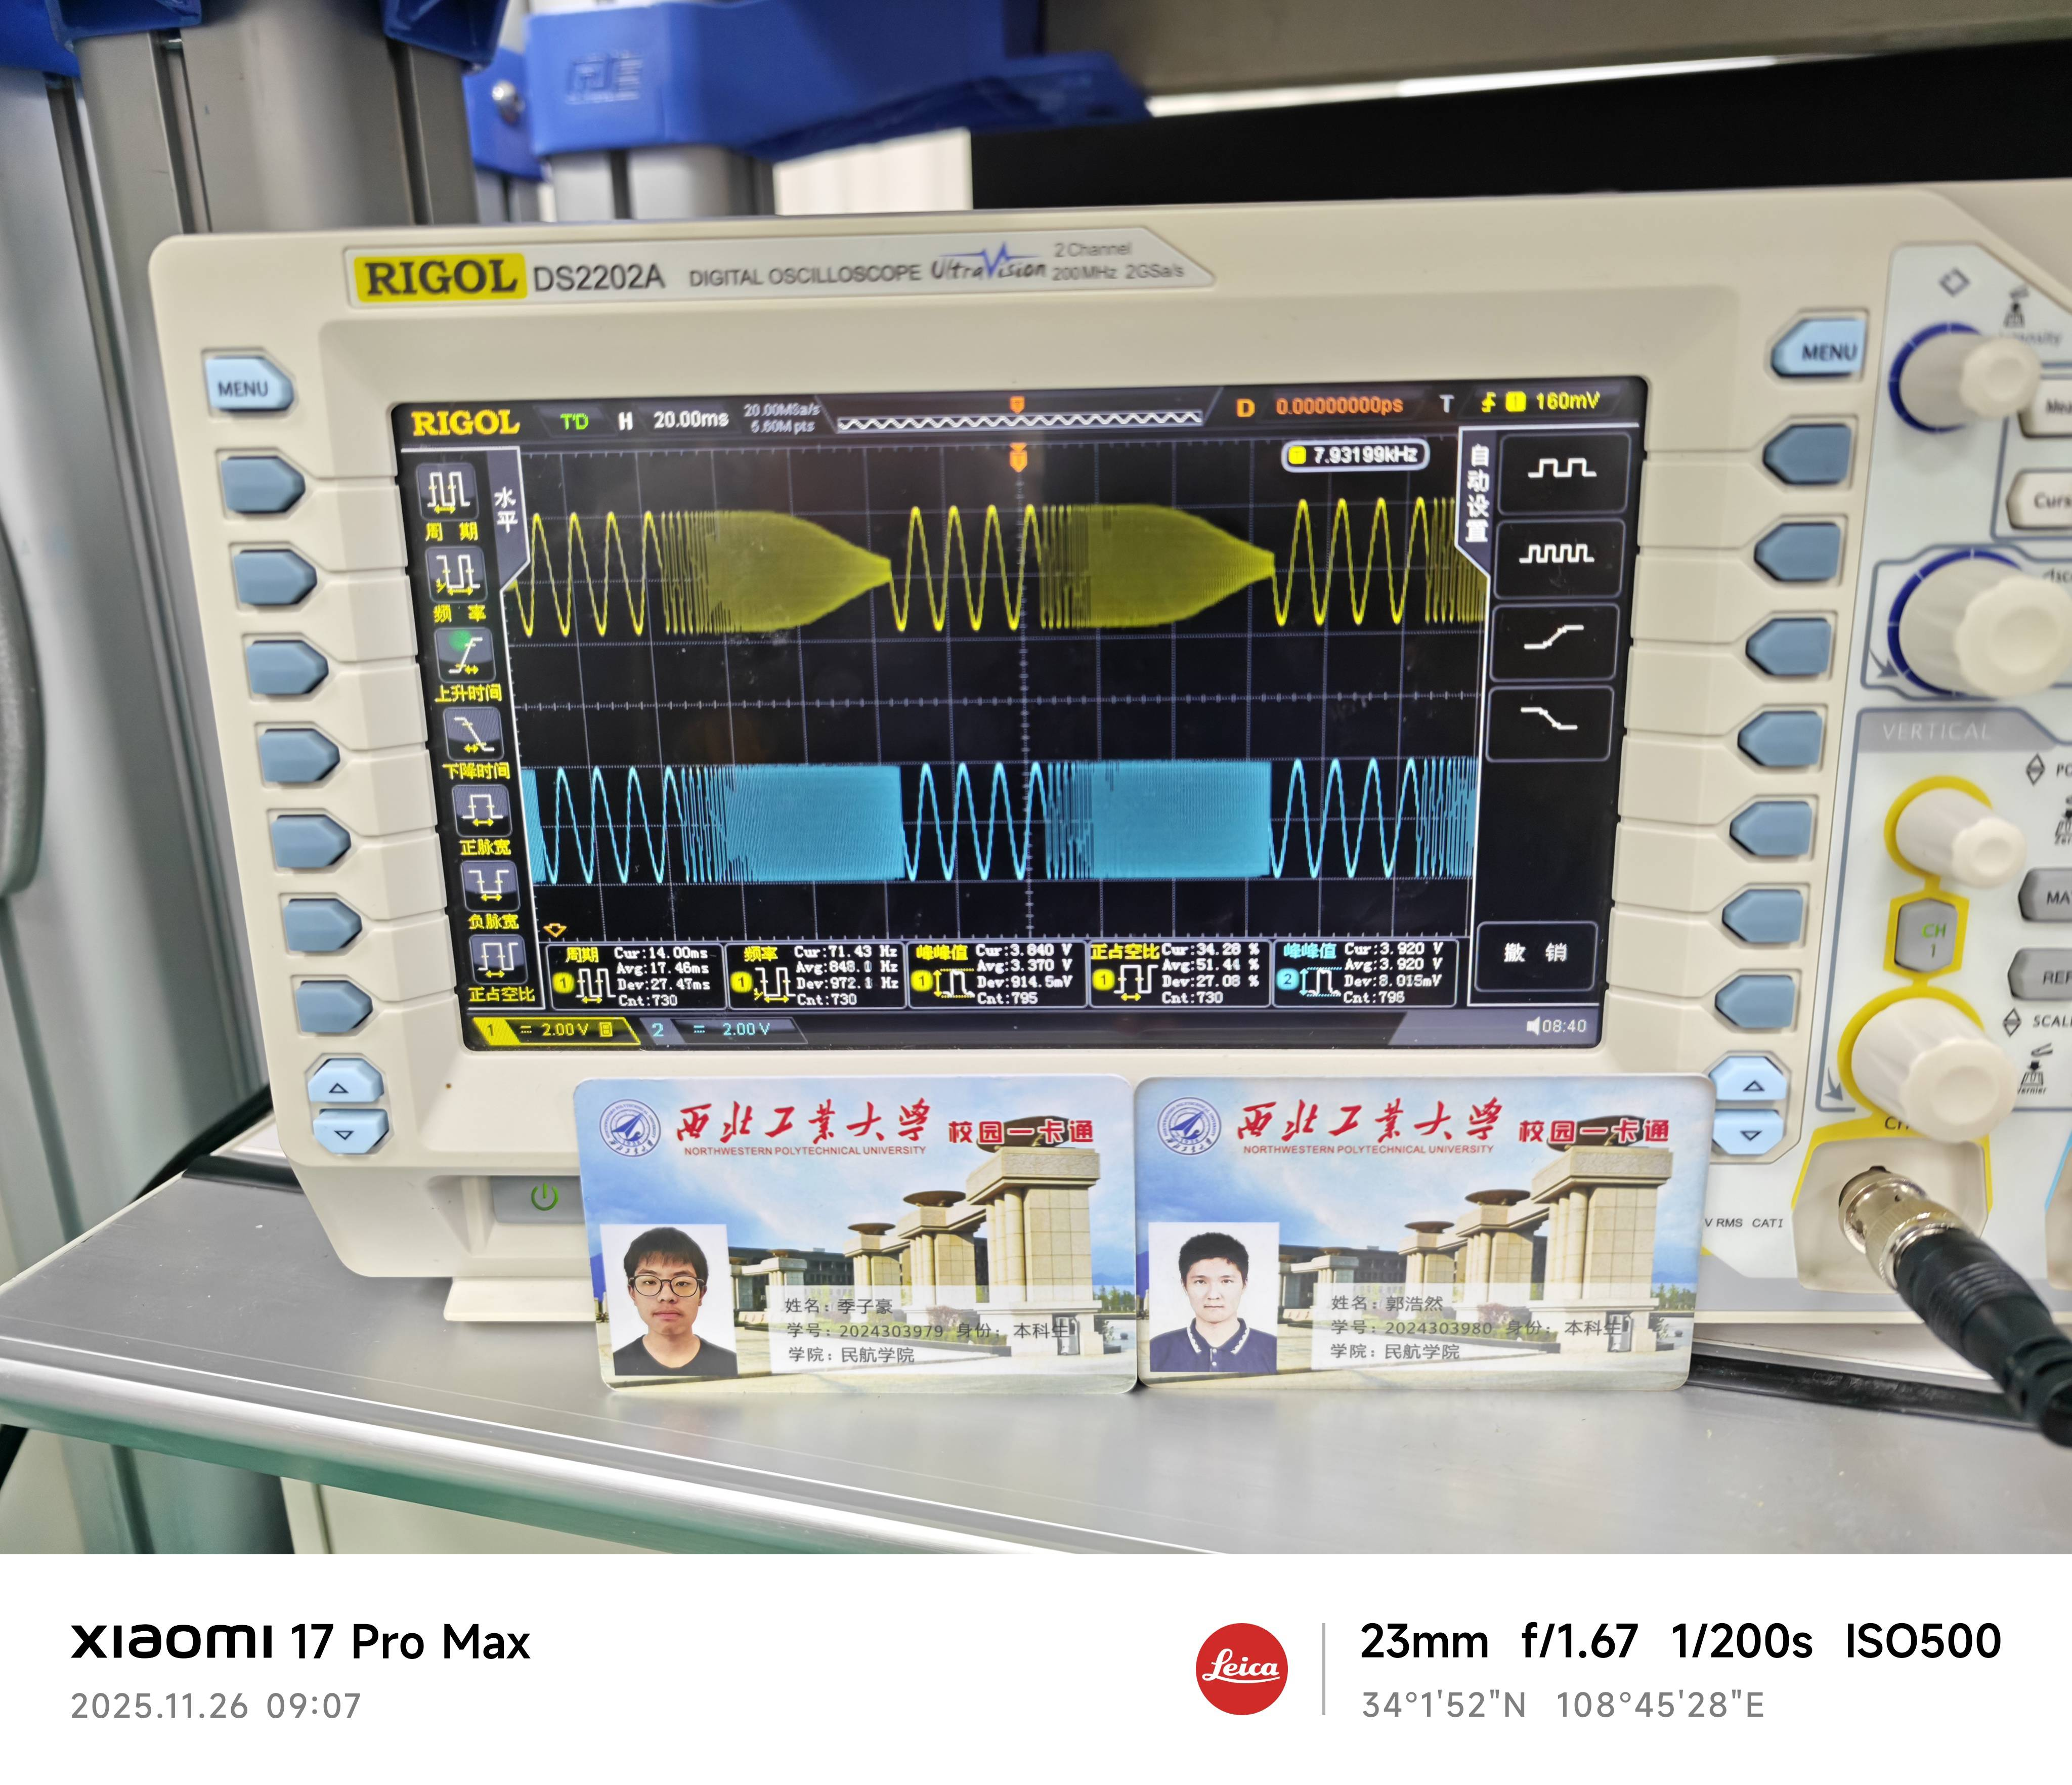
\includegraphics[width=\textwidth]{./4. frequency/figures/无源低通.jpg}
        \caption{无源低通扫频波形}
    \end{subfigure}
    \hfill
    \begin{subfigure}[b]{0.45\textwidth}
        \centering
        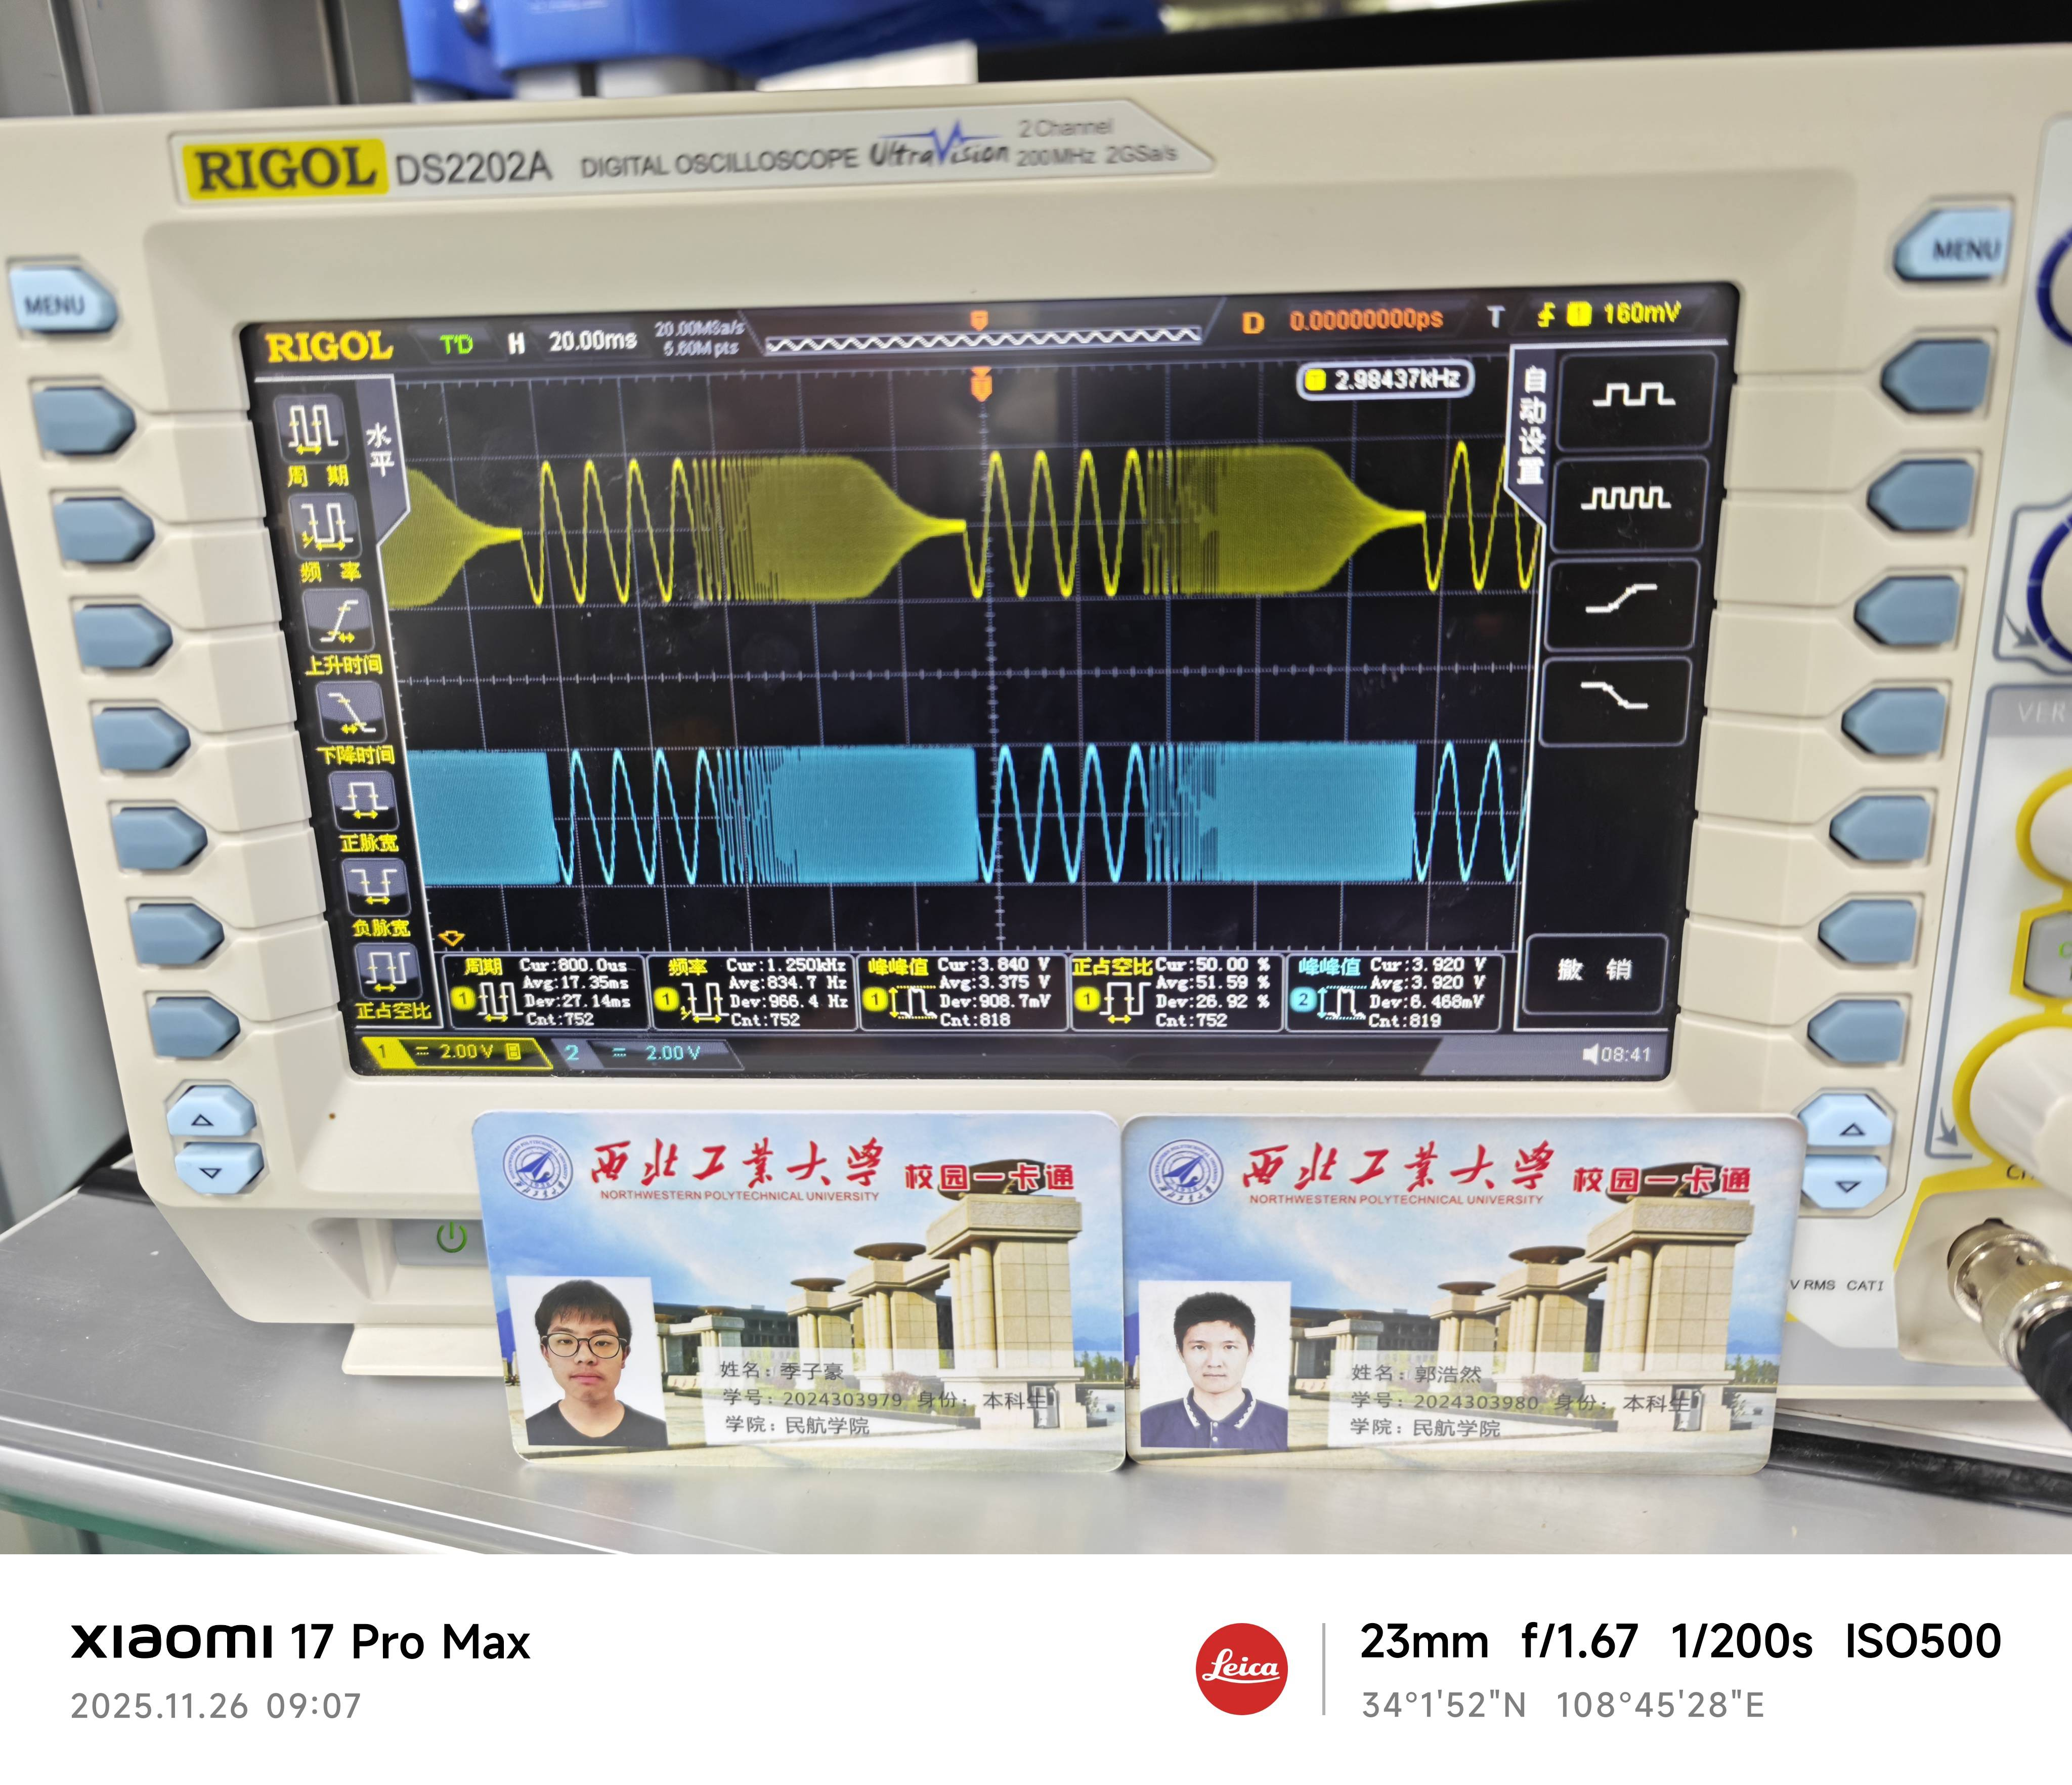
\includegraphics[width=\textwidth]{./4. frequency/figures/有源低通.jpg}
        \caption{有源低通扫频波形}
    \end{subfigure}
    \caption{低通滤波器实验结果综合展示}
\end{figure}

\newpage

% ---------------------------------------------------------
% 任务二：高通滤波器
% ---------------------------------------------------------
\subsection{任务二：测量高通滤波器的频响特性}

\subsubsection{逐点测量法数据}

\textbf{1. 无源高通滤波器}

\mygridtable{
    \begin{tabular}{|c|c|c|c|c|c|c|c|c|c|c|c|}
        \hline
        $V_i$ (V) & 4 & 4 & 4 & 4 & 4 & 4 & 4 & 4 & 4 & 4 & 4 \\
        \hline
        $f$ (Hz) & 100 & 1k & 5k & 10k & 15k & \textbf{17.2k} & 20k & 25k & 30k & 50k & 100k \\
        \hline
        $V_o$ (V) & 0.24 & 0.24 & 1.20 & 2.00 & 2.64 & \textbf{2.80} & 2.96 & 3.12 & 3.28 & 3.52 & 3.60 \\
        \hline
        \multicolumn{12}{|l|}{\textbf{测量结论：} 当 $V_o \approx 2.828\,\mathrm{V}$ 时，测得截止频率 $f_L = 17.2\,\mathrm{kHz}$} \\
        \hline
    \end{tabular}
}{高通无源滤波器逐点测量数据}

\textbf{2. 有源高通滤波器}

\mygridtable{
    \begin{tabular}{|c|c|c|c|c|c|c|c|c|c|c|c|}
        \hline
        $V_i$ (V) & 4 & 4 & 4 & 4 & 4 & 4 & 4 & 4 & 4 & 4 & 4 \\
        \hline
        $f$ (Hz) & 100 & 1k & 5k & 10k & 15k & \textbf{17.0k} & 20k & 25k & 30k & 50k & 100k \\
        \hline
        $V_o$ (V) & 0.24 & 0.24 & 0.88 & 2.00 & 2.64 & \textbf{2.80} & 2.96 & 3.20 & 3.28 & 3.52 & 3.60 \\
        \hline
        \multicolumn{12}{|l|}{\textbf{测量结论：} 当 $V_o \approx 2.828\,\mathrm{V}$ 时，测得截止频率 $f_L = 17.0\,\mathrm{kHz}$} \\
        \hline
    \end{tabular}
}{高通有源滤波器逐点测量数据}

\subsubsection{幅频特性曲线与扫频测试}

\begin{figure}[H]
    \centering
    \begin{subfigure}[b]{0.8\textwidth}
        \centering
        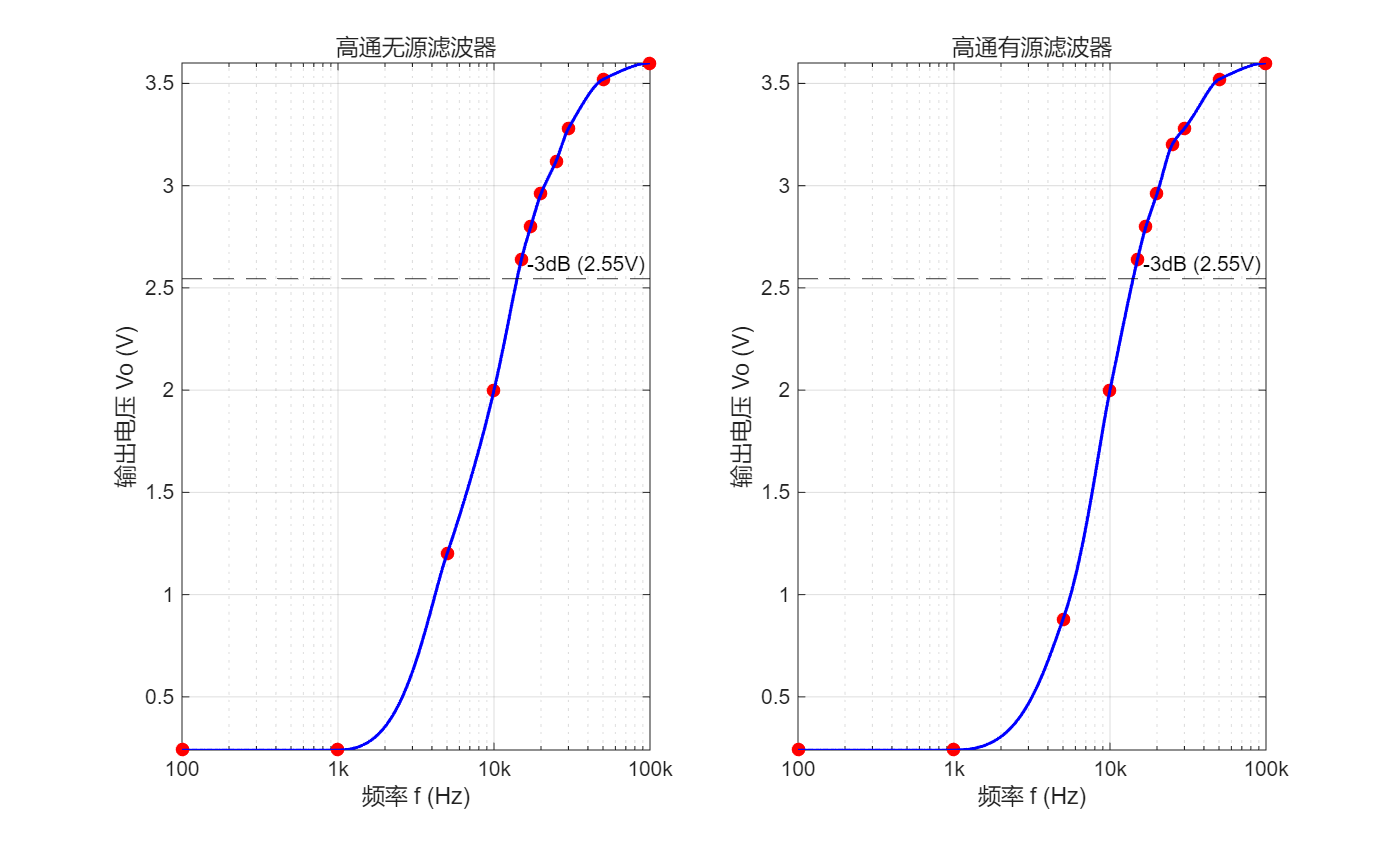
\includegraphics[width=\textwidth]{./4. frequency/figures/高通.png}
        \caption{高通滤波器幅频特性曲线 (MATLAB)}
    \end{subfigure}
    
    \vspace{1em}
    
    \begin{subfigure}[b]{0.45\textwidth}
        \centering
        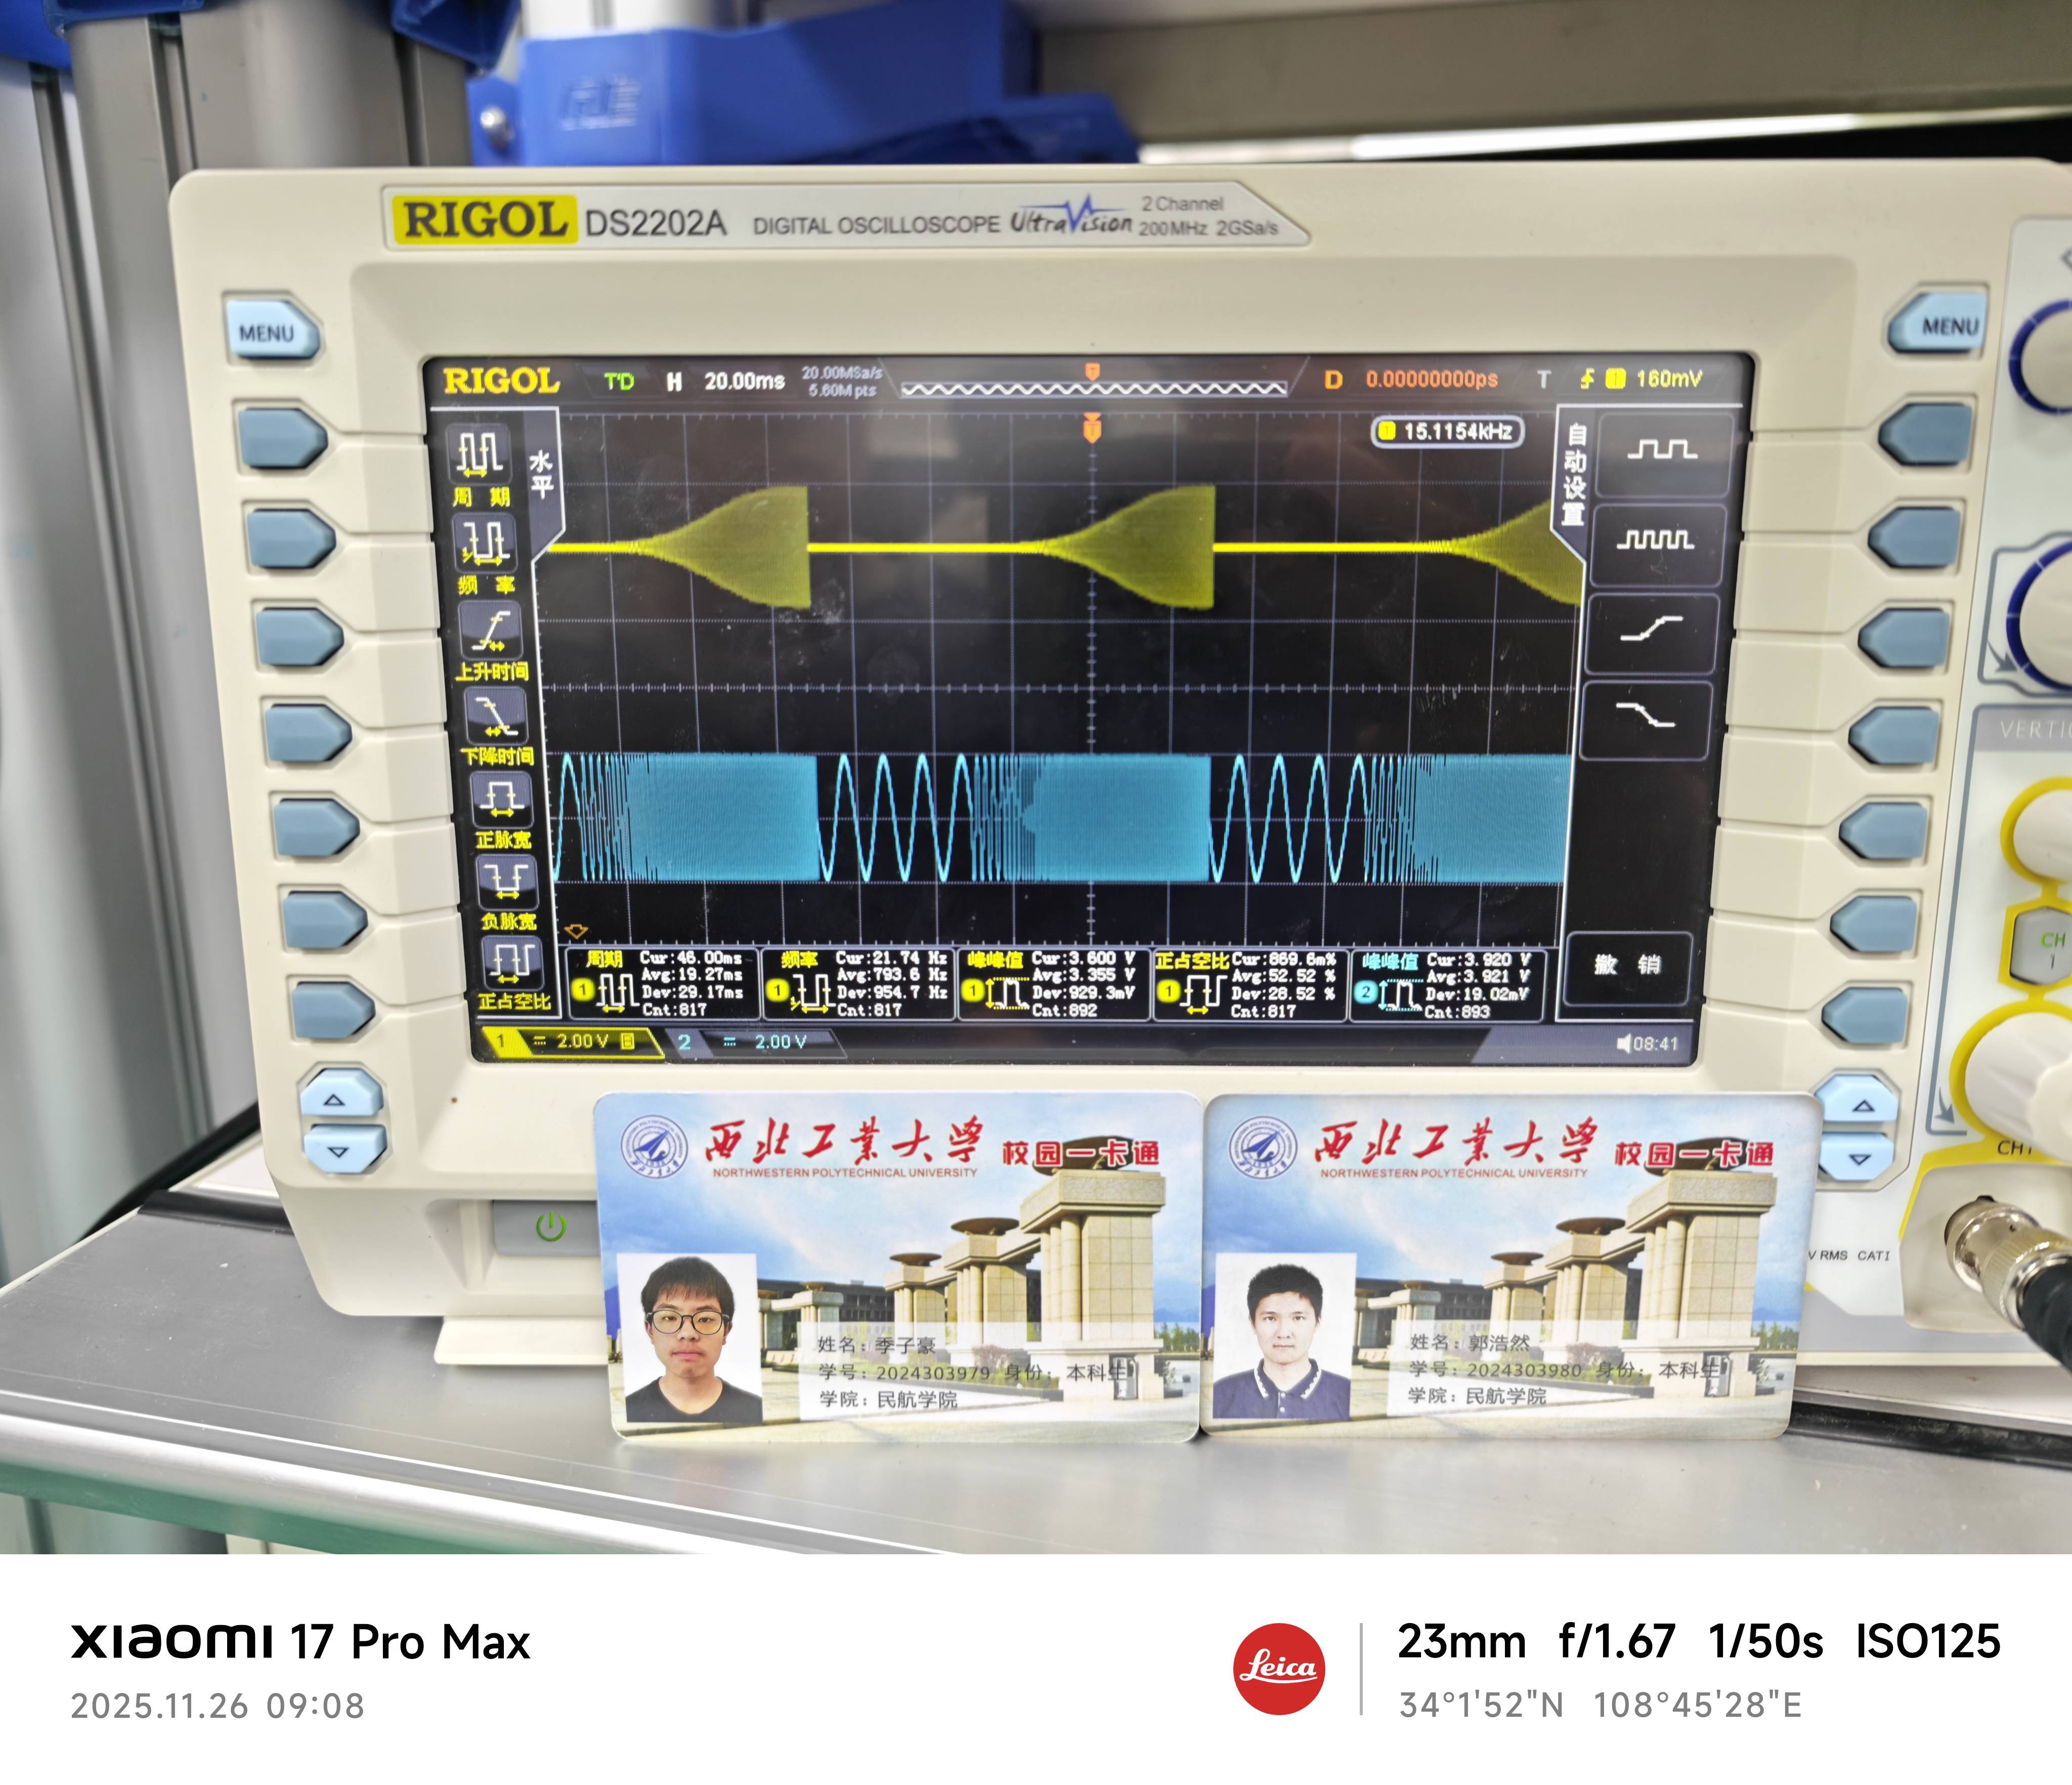
\includegraphics[width=\textwidth]{./4. frequency/figures/无源高通.jpg}
        \caption{无源高通扫频波形}
    \end{subfigure}
    \hfill
    \begin{subfigure}[b]{0.45\textwidth}
        \centering
        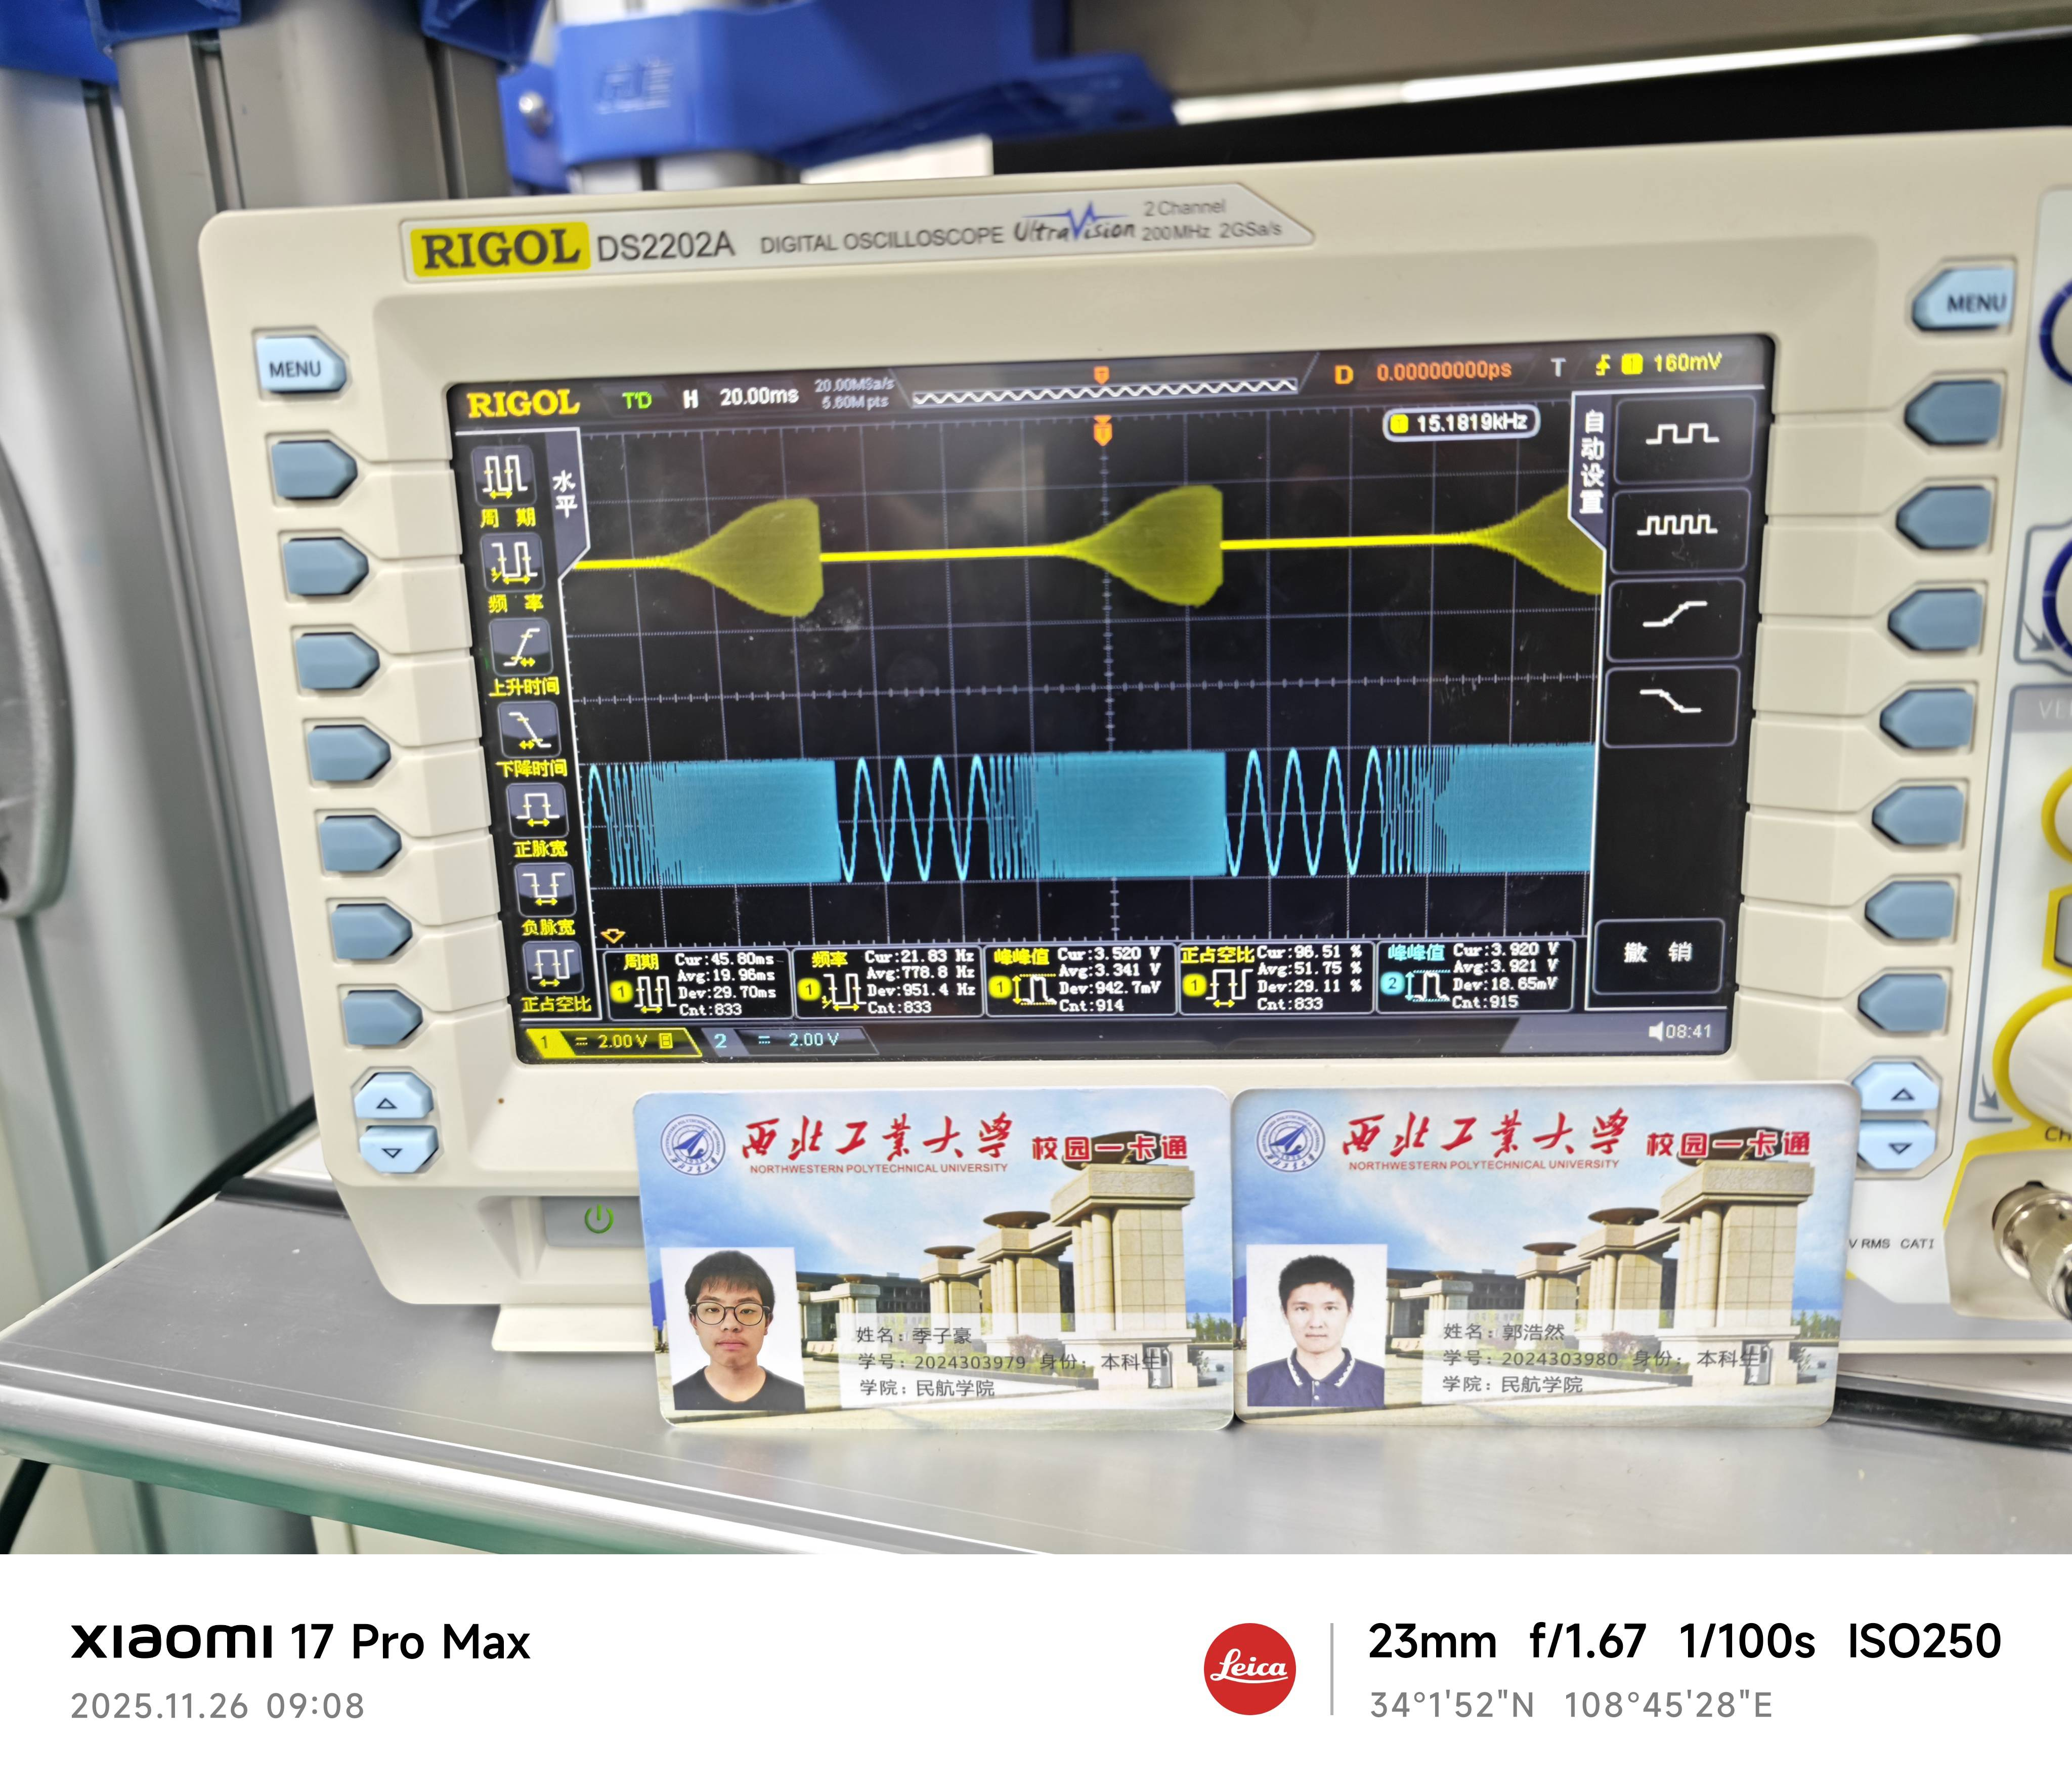
\includegraphics[width=\textwidth]{./4. frequency/figures/有源高通.jpg}
        \caption{有源高通扫频波形}
    \end{subfigure}
    \caption{高通滤波器实验结果综合展示}
\end{figure}

\newpage

% ---------------------------------------------------------
% 任务三：带通滤波器
% ---------------------------------------------------------
\subsection{任务三：测量带通滤波器的频响特性}

\subsubsection{逐点测量法数据}

\textbf{1. 无源带通滤波器}

\mygridtable{
    \begin{tabular}{|c|c|c|c|c|c|c|c|c|c|c|c|c|}
        \hline
        $V_i$ (V) & 4 & 4 & 4 & 4 & 4 & 4 & 4 & 4 & 4 & 4 & 4 & 4 \\
        \hline
        $f$ (Hz) & 100 & 1k & \textbf{2.1k} & 5k & 10k & \textbf{13k} & 15k & 20k & 25k & 30k & 50k & 100k \\
        \hline
        $V_o$ (V) & 0.40 & 2.00 & \textbf{2.80} & 3.20 & 3.04 & \textbf{2.80} & 2.72 & 2.40 & 2.16 & 1.84 & 1.36 & 0.72 \\
        \hline
        \multicolumn{13}{|l|}{\textbf{测量结论：}  $f_L = 2.1\,\mathrm{kHz}$， $f_H = 13.0\,\mathrm{kHz}$} \\
        \hline
    \end{tabular}
}{带通无源滤波器逐点测量数据}

\textbf{2. 有源带通滤波器}

\mygridtable{
    \begin{tabular}{|c|c|c|c|c|c|c|c|c|c|c|c|}
        \hline
        $V_i$ (V) & 4 & 4 & 4 & 4 & 4 & 4 & 4 & 4 & 4 & 4 & 4 \\
        \hline
        $f$ (Hz) & 100 & 1k & \textbf{3.8k} & 5k & 10k & \textbf{15k} & 20k & 25k & 30k & 50k & 100k \\
        \hline
        $V_o$ (V) & 0.24 & 1.20 & \textbf{2.80} & 3.04 & 3.12 & \textbf{2.80} & 2.48 & 2.16 & 1.84 & 1.28 & 0.72 \\
        \hline
        \multicolumn{12}{|l|}{\textbf{测量结论：}  $f_L = 3.8\,\mathrm{kHz}$， $f_H = 15.0\,\mathrm{kHz}$} \\
        \hline
    \end{tabular}
}{带通有源滤波器逐点测量数据}

\subsubsection{幅频特性曲线与扫频测试}

\begin{figure}[H]
    \centering
    \begin{subfigure}[b]{0.8\textwidth}
        \centering
        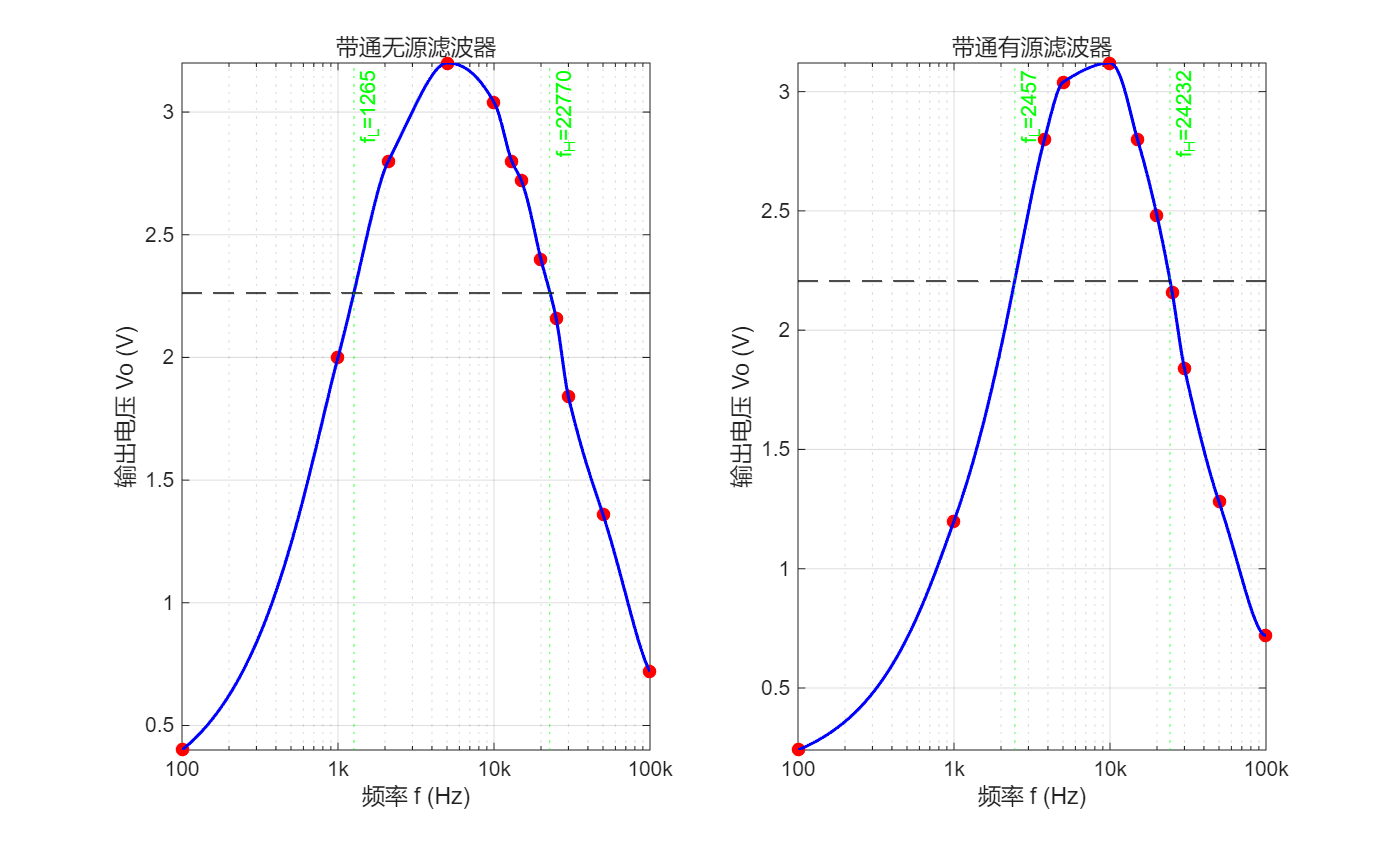
\includegraphics[width=\textwidth]{./4. frequency/figures/带通.png}
        \caption{带通滤波器幅频特性曲线 (MATLAB)}
    \end{subfigure}
    
    \vspace{1em}
    
    \begin{subfigure}[b]{0.45\textwidth}
        \centering
        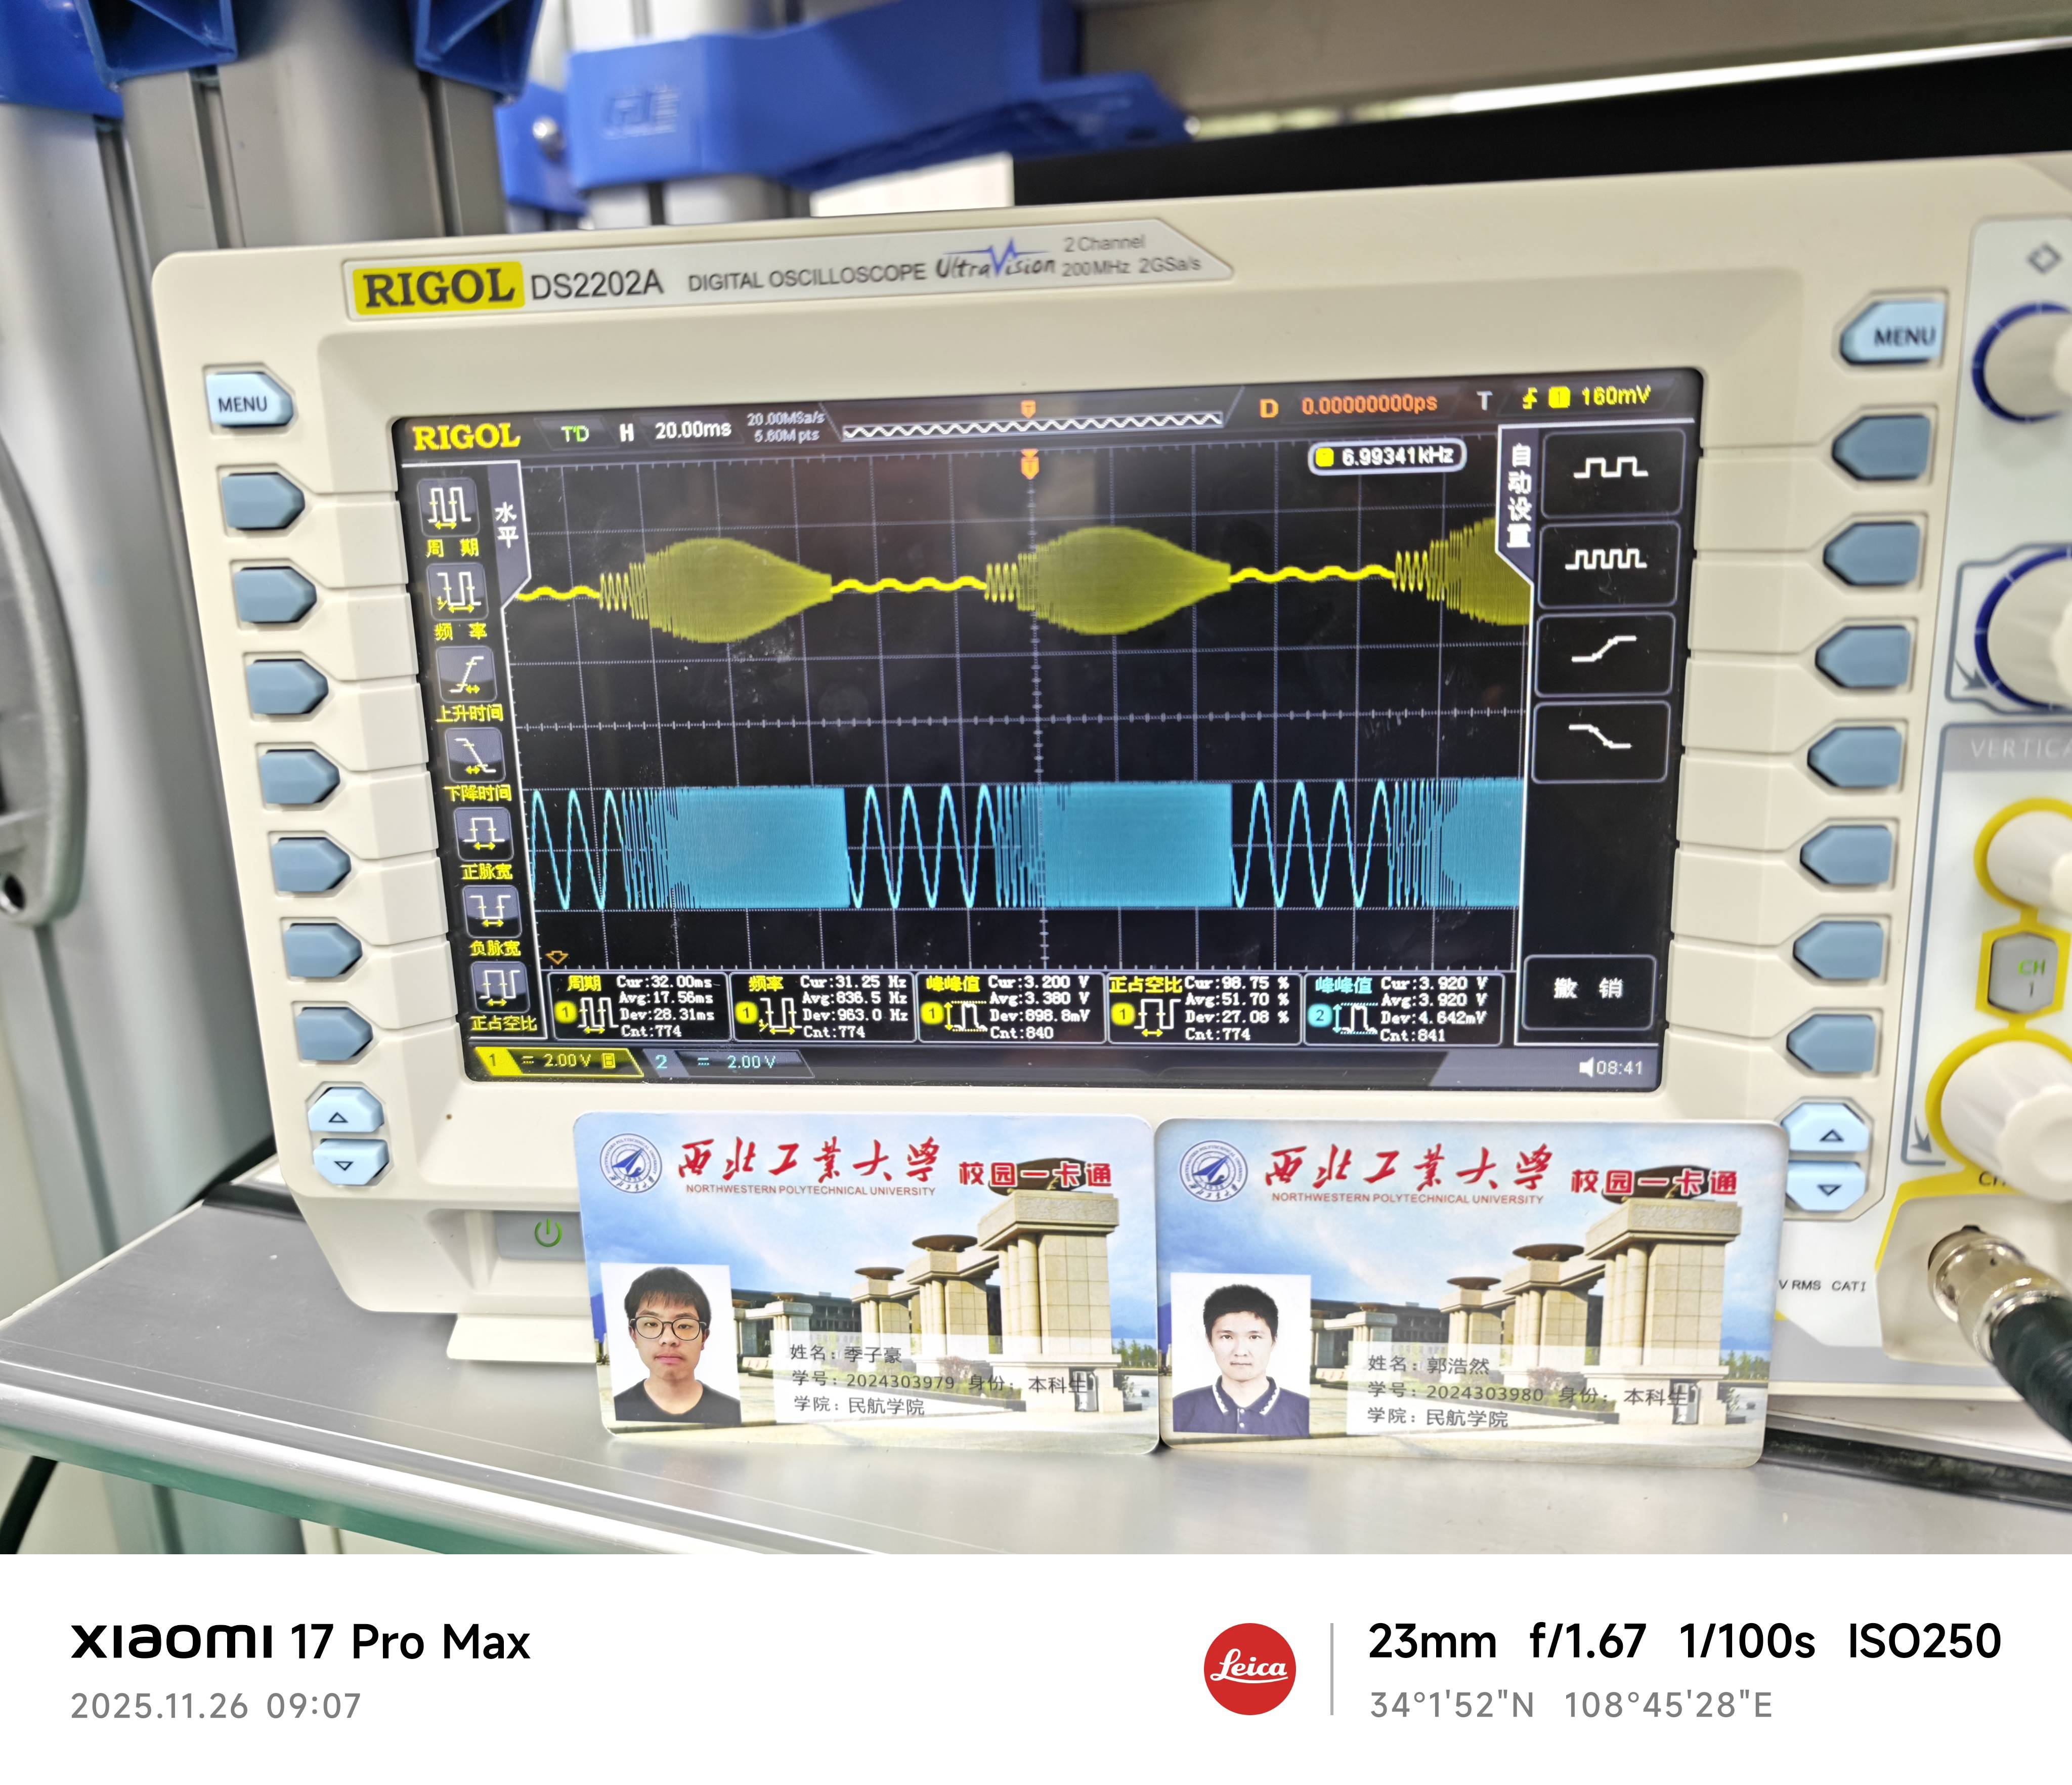
\includegraphics[width=\textwidth]{./4. frequency/figures/无源带通.jpg}
        \caption{无源带通扫频波形}
    \end{subfigure}
    \hfill
    \begin{subfigure}[b]{0.45\textwidth}
        \centering
        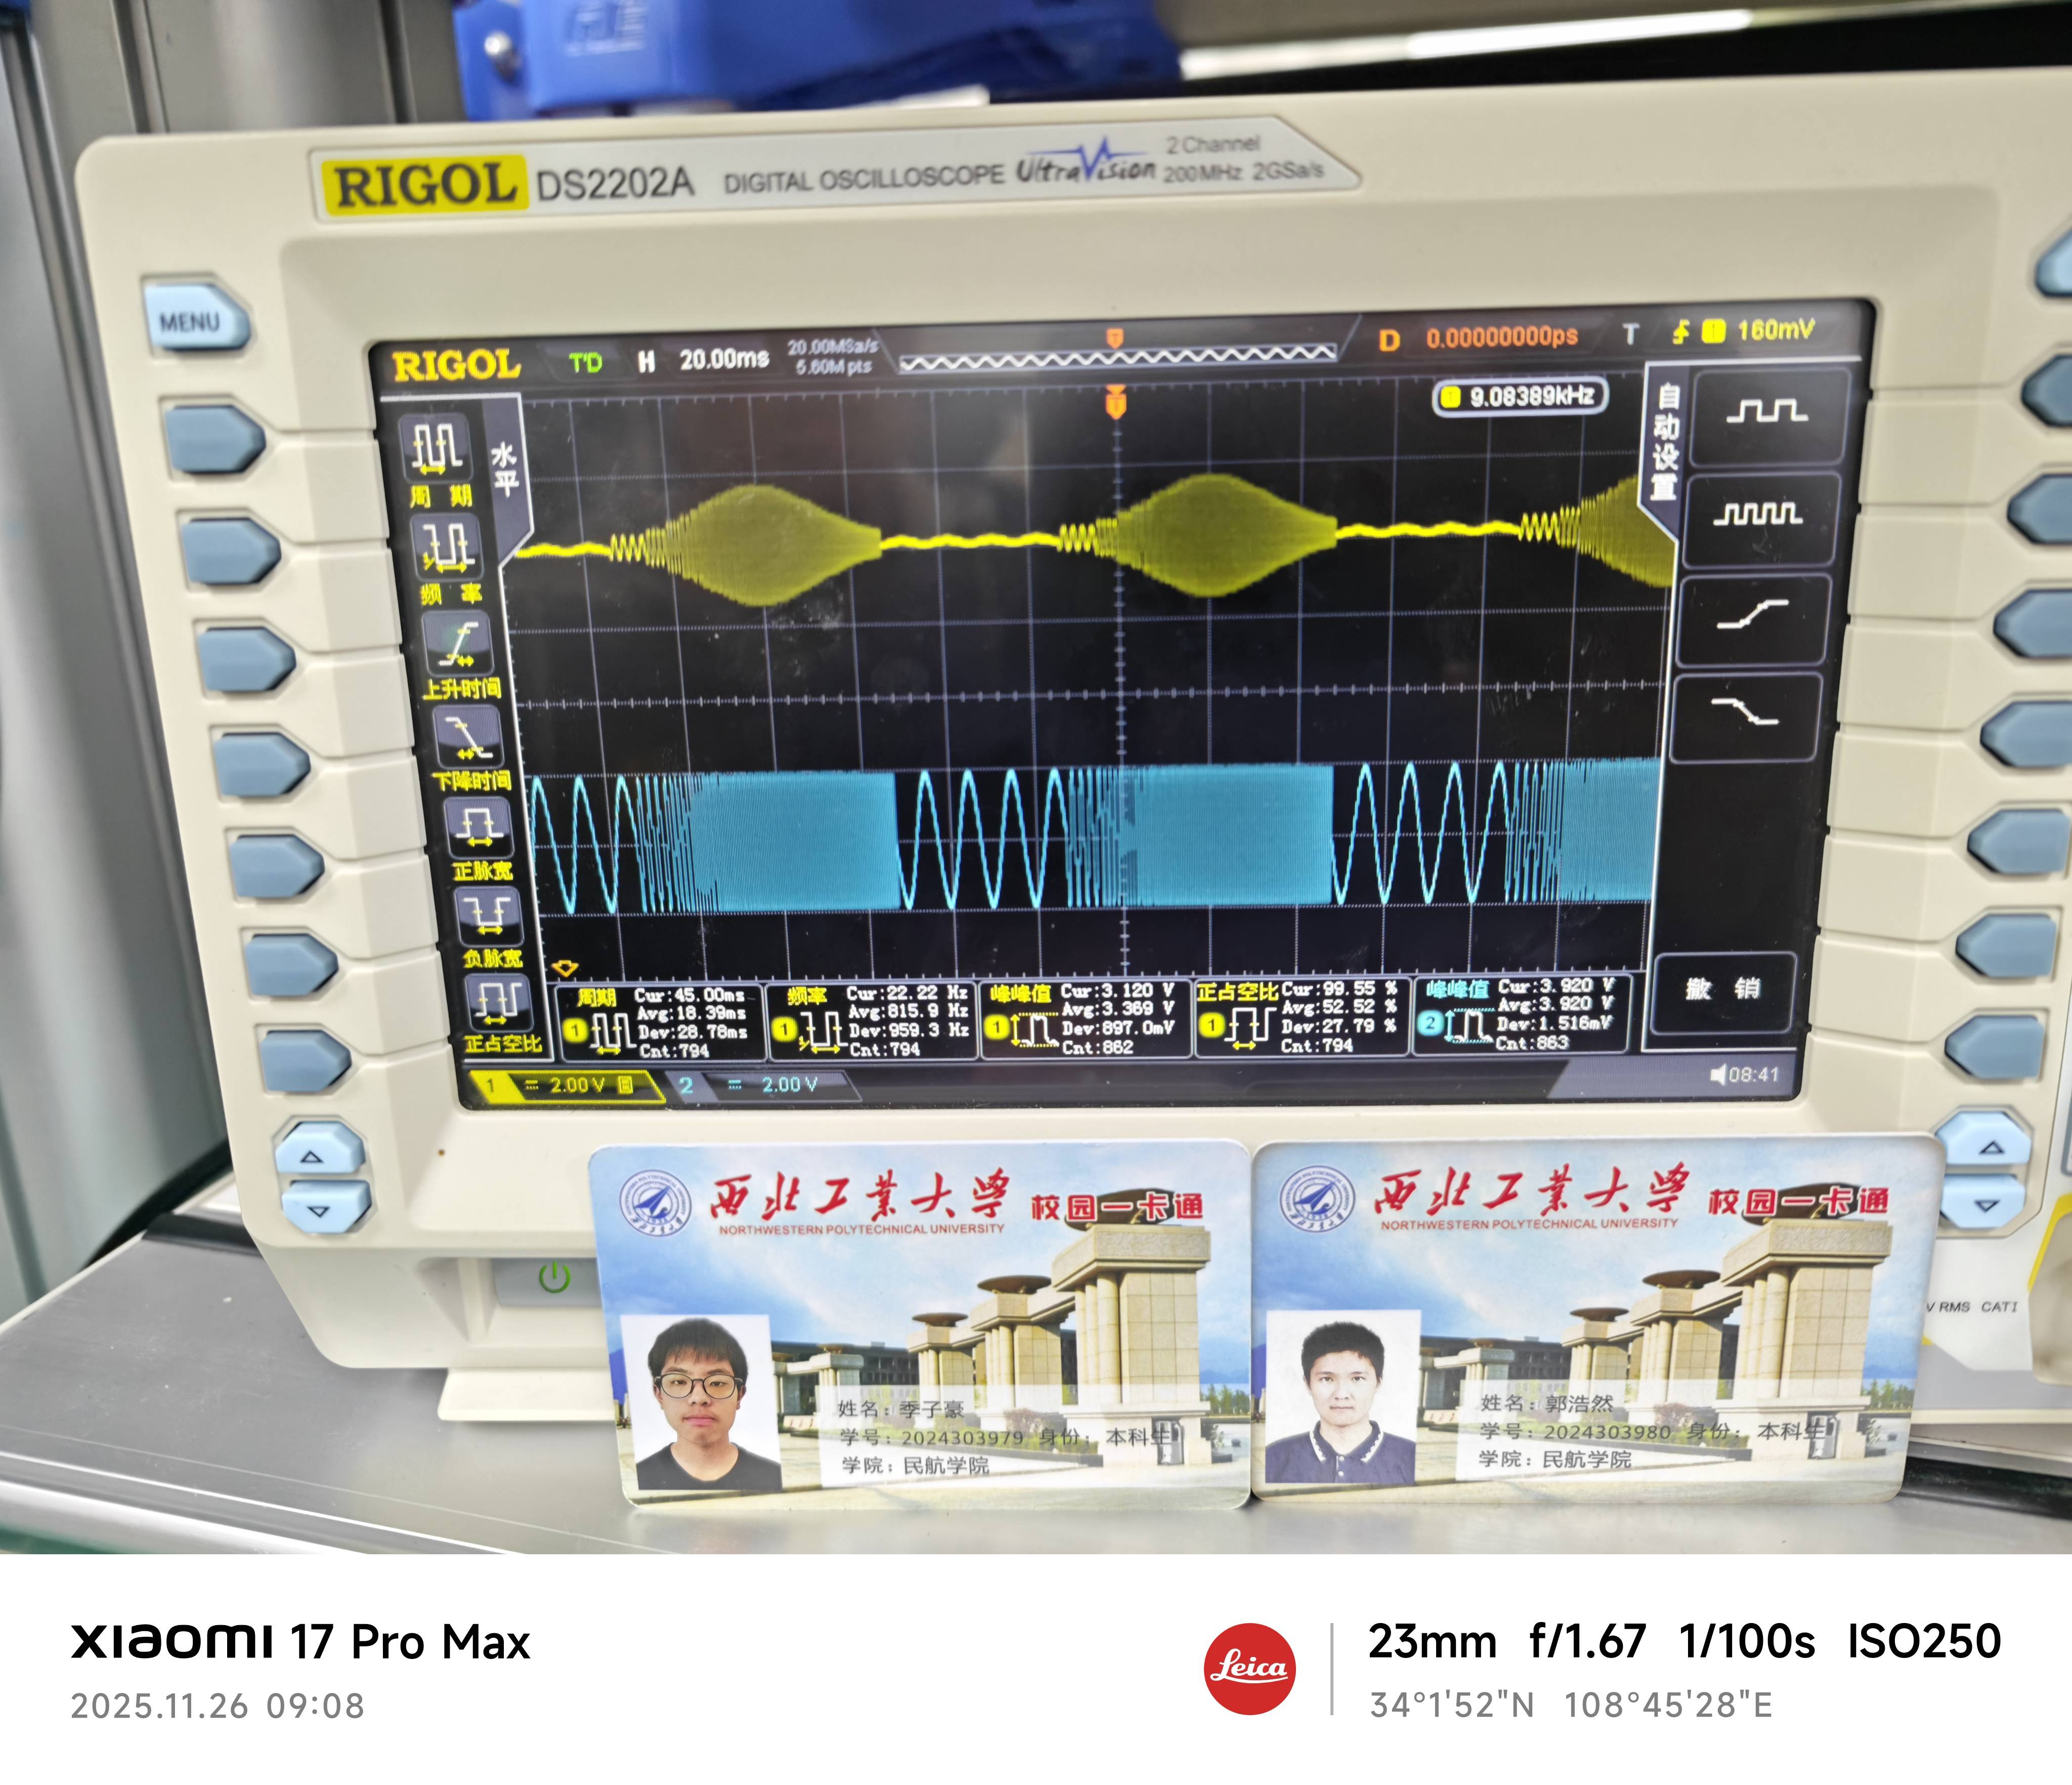
\includegraphics[width=\textwidth]{./4. frequency/figures/有源带通.jpg}
        \caption{有源带通扫频波形}
    \end{subfigure}
    \caption{带通滤波器实验结果综合展示}
\end{figure}

\newpage

% ---------------------------------------------------------
% 任务四：带阻滤波器
% ---------------------------------------------------------
\subsection{任务四：测量带阻滤波器的频响特性}

\subsubsection{逐点测量法数据}

\textbf{1. 无源带阻滤波器}

\mygridtable{
    \begin{tabular}{|c|c|c|c|c|c|c|c|c|c|c|c|c|c|c|c|c|c|}
        \hline
        $V_i$ (V) & 4 & 4 & 4 & 4 & 4 & 4 & 4 & 4 & 4 & 4 & 4 & 4 & 4 & 4 & 4 & 4 & 4 \\
        \hline
        $f$ (Hz) & 100 & 500 & 1k & 3k & \textbf{3.6k} & 5k & 10k & 15k & 20k & 25k & 30k & 40k & 50k & 60k & 80k & \textbf{85k} & 100k \\
        \hline
        $V_o$ (V) & 3.84 & 3.84 & 3.68 & 3.04 & \textbf{2.80} & 2.32 & 1.04 & 0.32 & 0.48 & 0.88 & 1.28 & 1.76 & 2.08 & 2.40 & 2.72 & \textbf{2.80} & 2.96 \\
        \hline
        \multicolumn{18}{|l|}{\textbf{测量结论：}  $f_L = 3.6\,\mathrm{kHz}$， $f_H = 85.0\,\mathrm{kHz}$} \\
        \hline
    \end{tabular}
}{带阻无源滤波器逐点测量数据}

\textbf{2. 有源带阻滤波器}

\mygridtable{
    \begin{tabular}{|c|c|c|c|c|c|c|c|c|c|c|c|c|c|c|}
        \hline
        $V_i$ (V) & 4 & 4 & 4 & 4 & 4 & 4 & 4 & 4 & 4 & 4 & 4 & 4 & 4 & 4 \\
        \hline
        $f$ (Hz) & 100 & 500 & 1k & 3k & 5k & \textbf{6.5k} & 10k & 15k & 20k & 25k & 30k & \textbf{45.8k} & 50k & 80k \\
        \hline
        $V_o$ (V) & 3.92 & 3.84 & 3.84 & 3.52 & 3.12 & \textbf{2.80} & 1.76 & 0.48 & 0.88 & 1.60 & 2.08 & \textbf{2.80} & 2.88 & 2.96 \\
        \hline
        \multicolumn{15}{|l|}{\textbf{测量结论：}  $f_L = 6.5\,\mathrm{kHz}$， $f_H = 45.8\,\mathrm{kHz}$} \\
        \hline
    \end{tabular}
}{带阻有源滤波器逐点测量数据}

\subsubsection{幅频特性曲线与扫频测试}

\begin{figure}[H]
    \centering
    \begin{subfigure}[b]{0.8\textwidth}
        \centering
        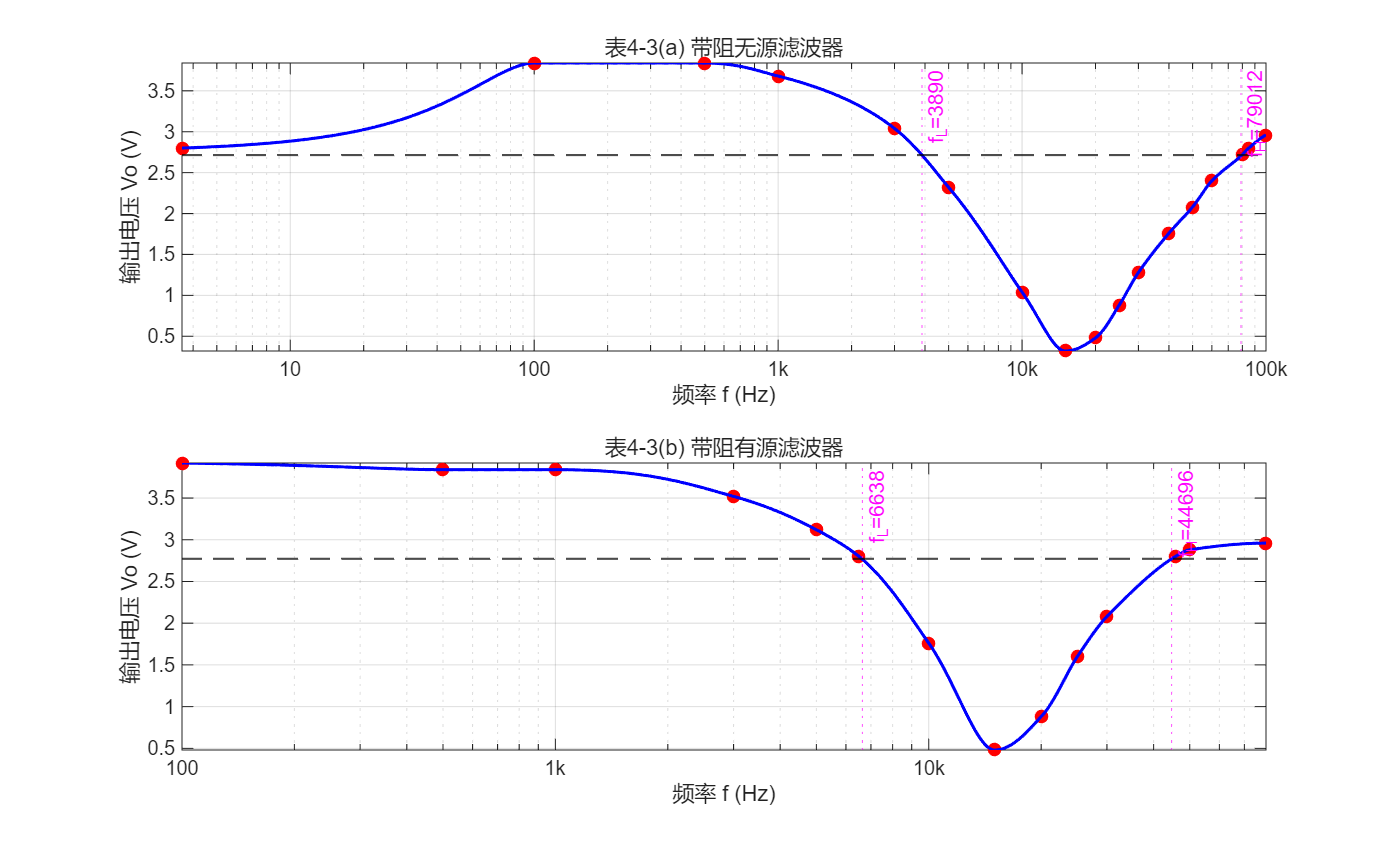
\includegraphics[width=\textwidth]{./4. frequency/figures/带阻.png}
        \caption{带阻滤波器幅频特性曲线 (MATLAB)}
    \end{subfigure}
    
    \vspace{1em}
    
    \begin{subfigure}[b]{0.45\textwidth}
        \centering
        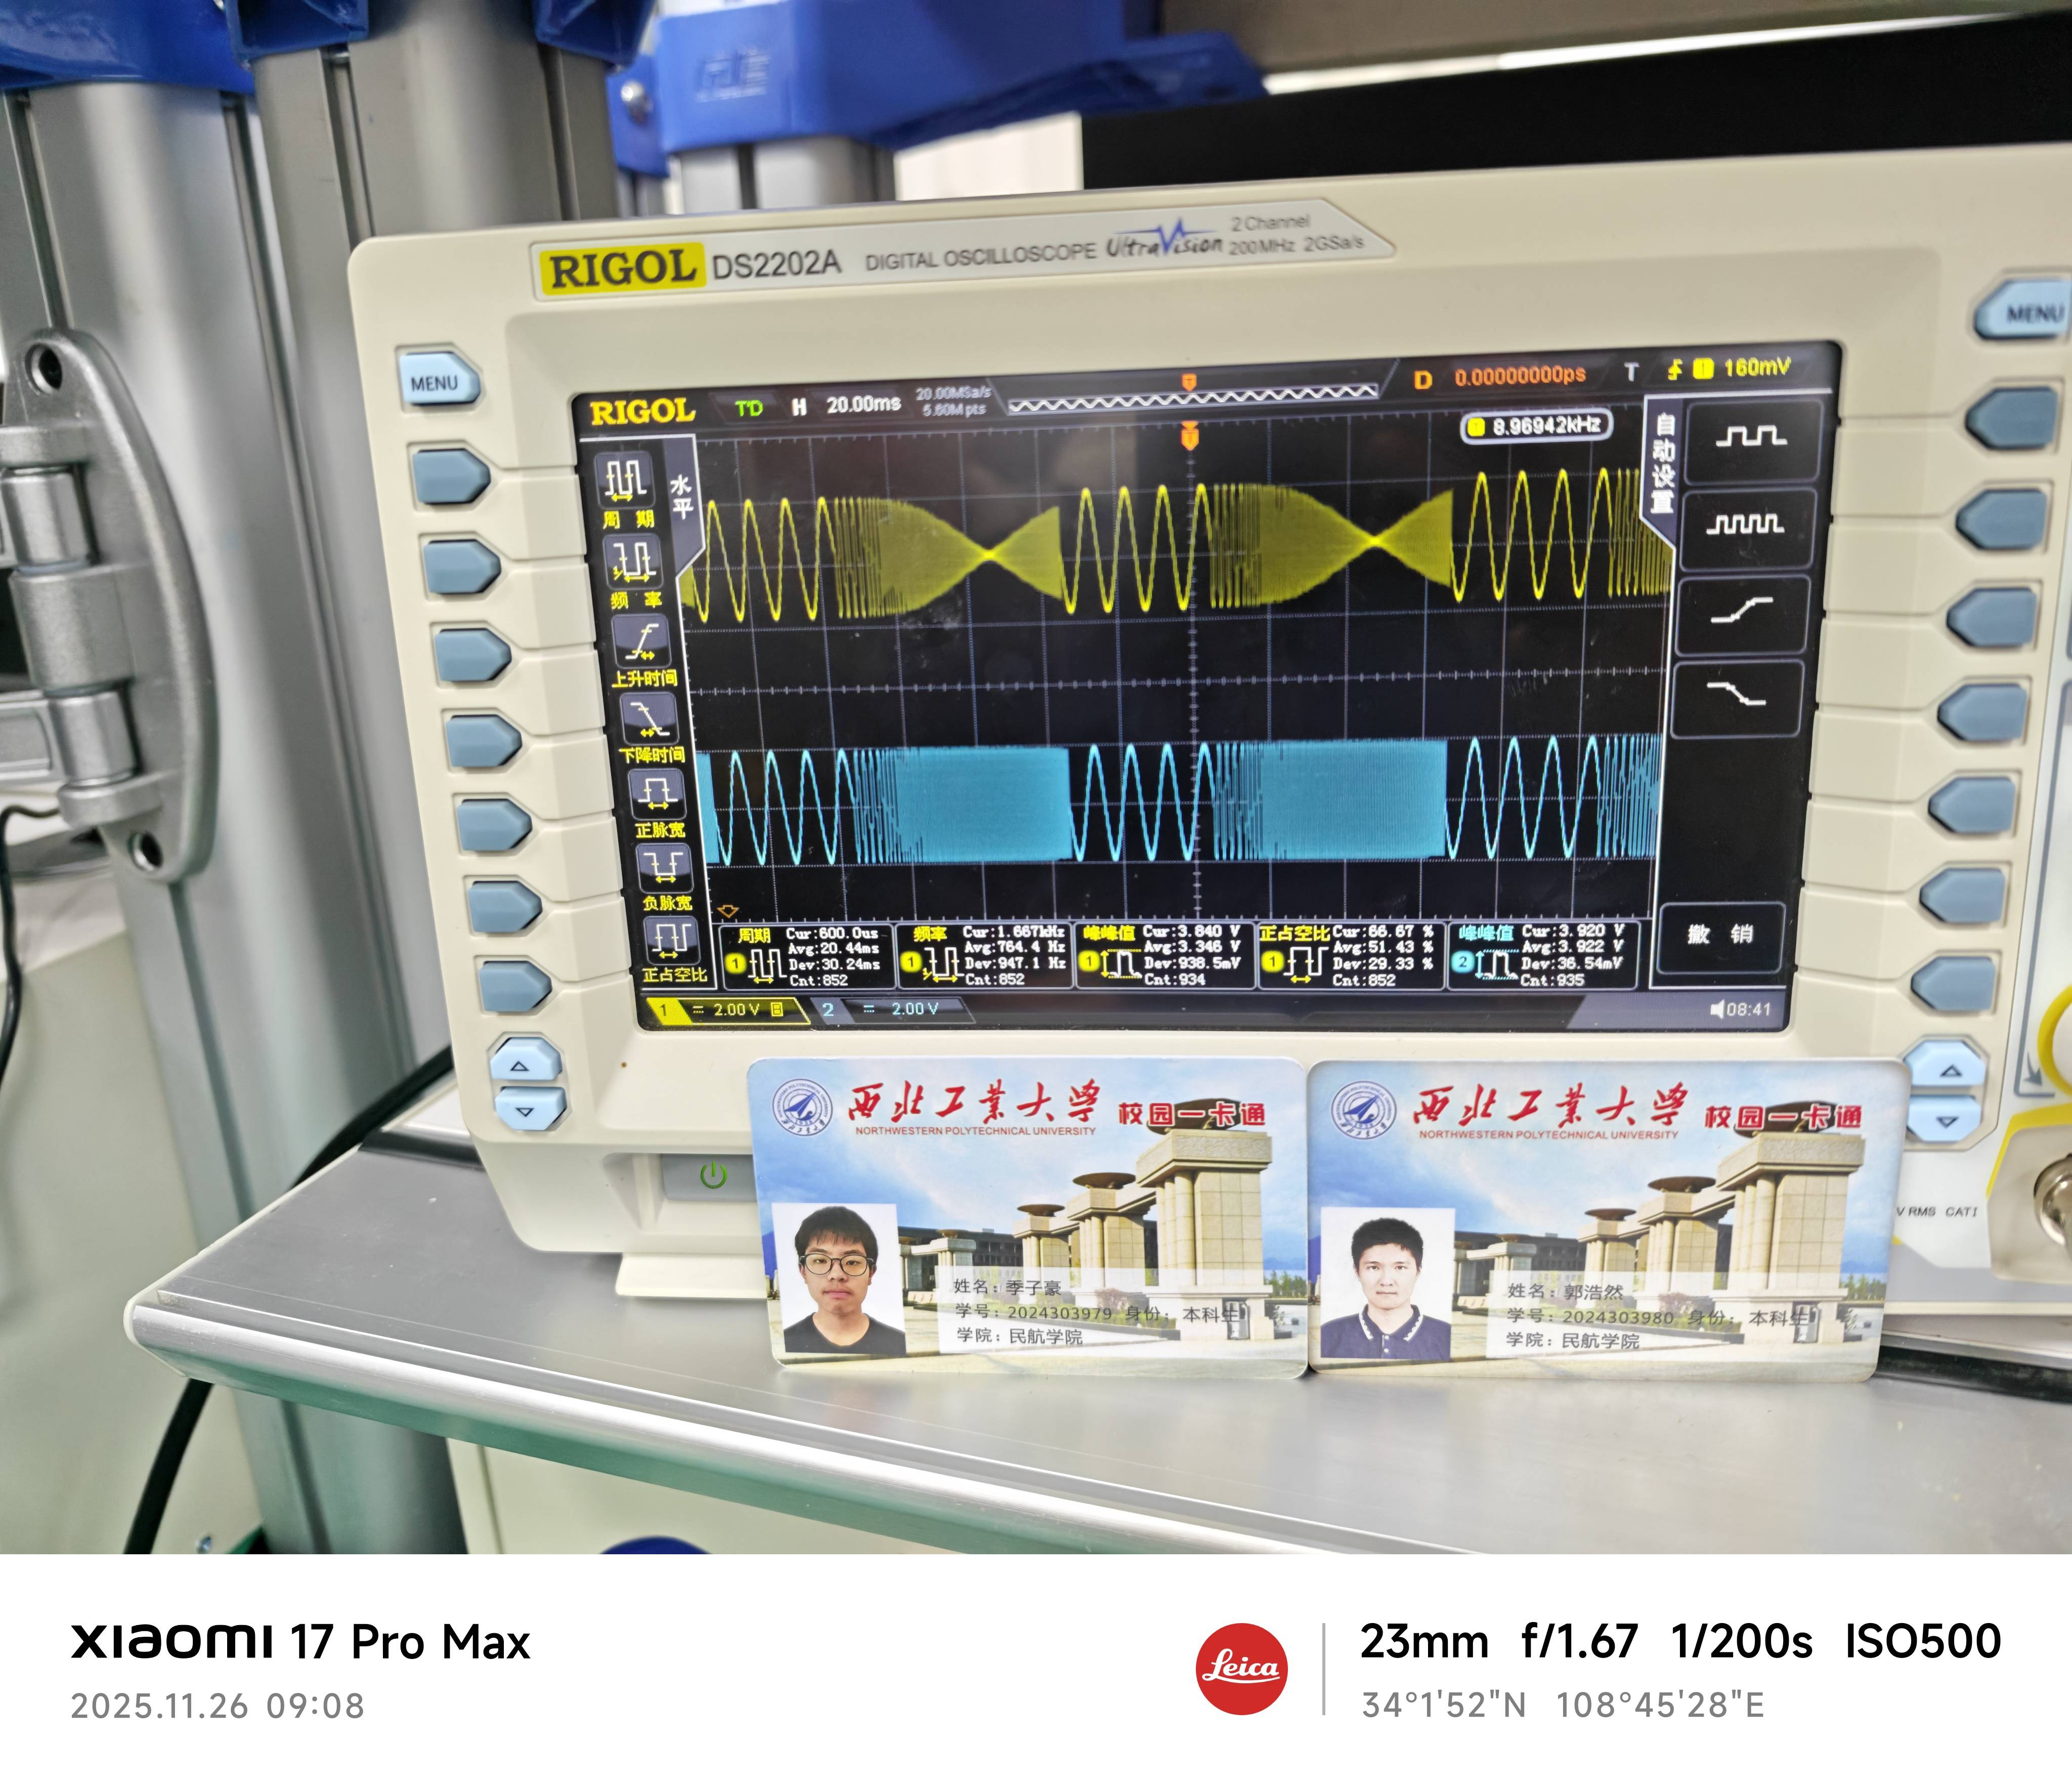
\includegraphics[width=\textwidth]{./4. frequency/figures/无源带阻.jpg}
        \caption{无源带阻扫频波形}
    \end{subfigure}
    \hfill
    \begin{subfigure}[b]{0.45\textwidth}
        \centering
        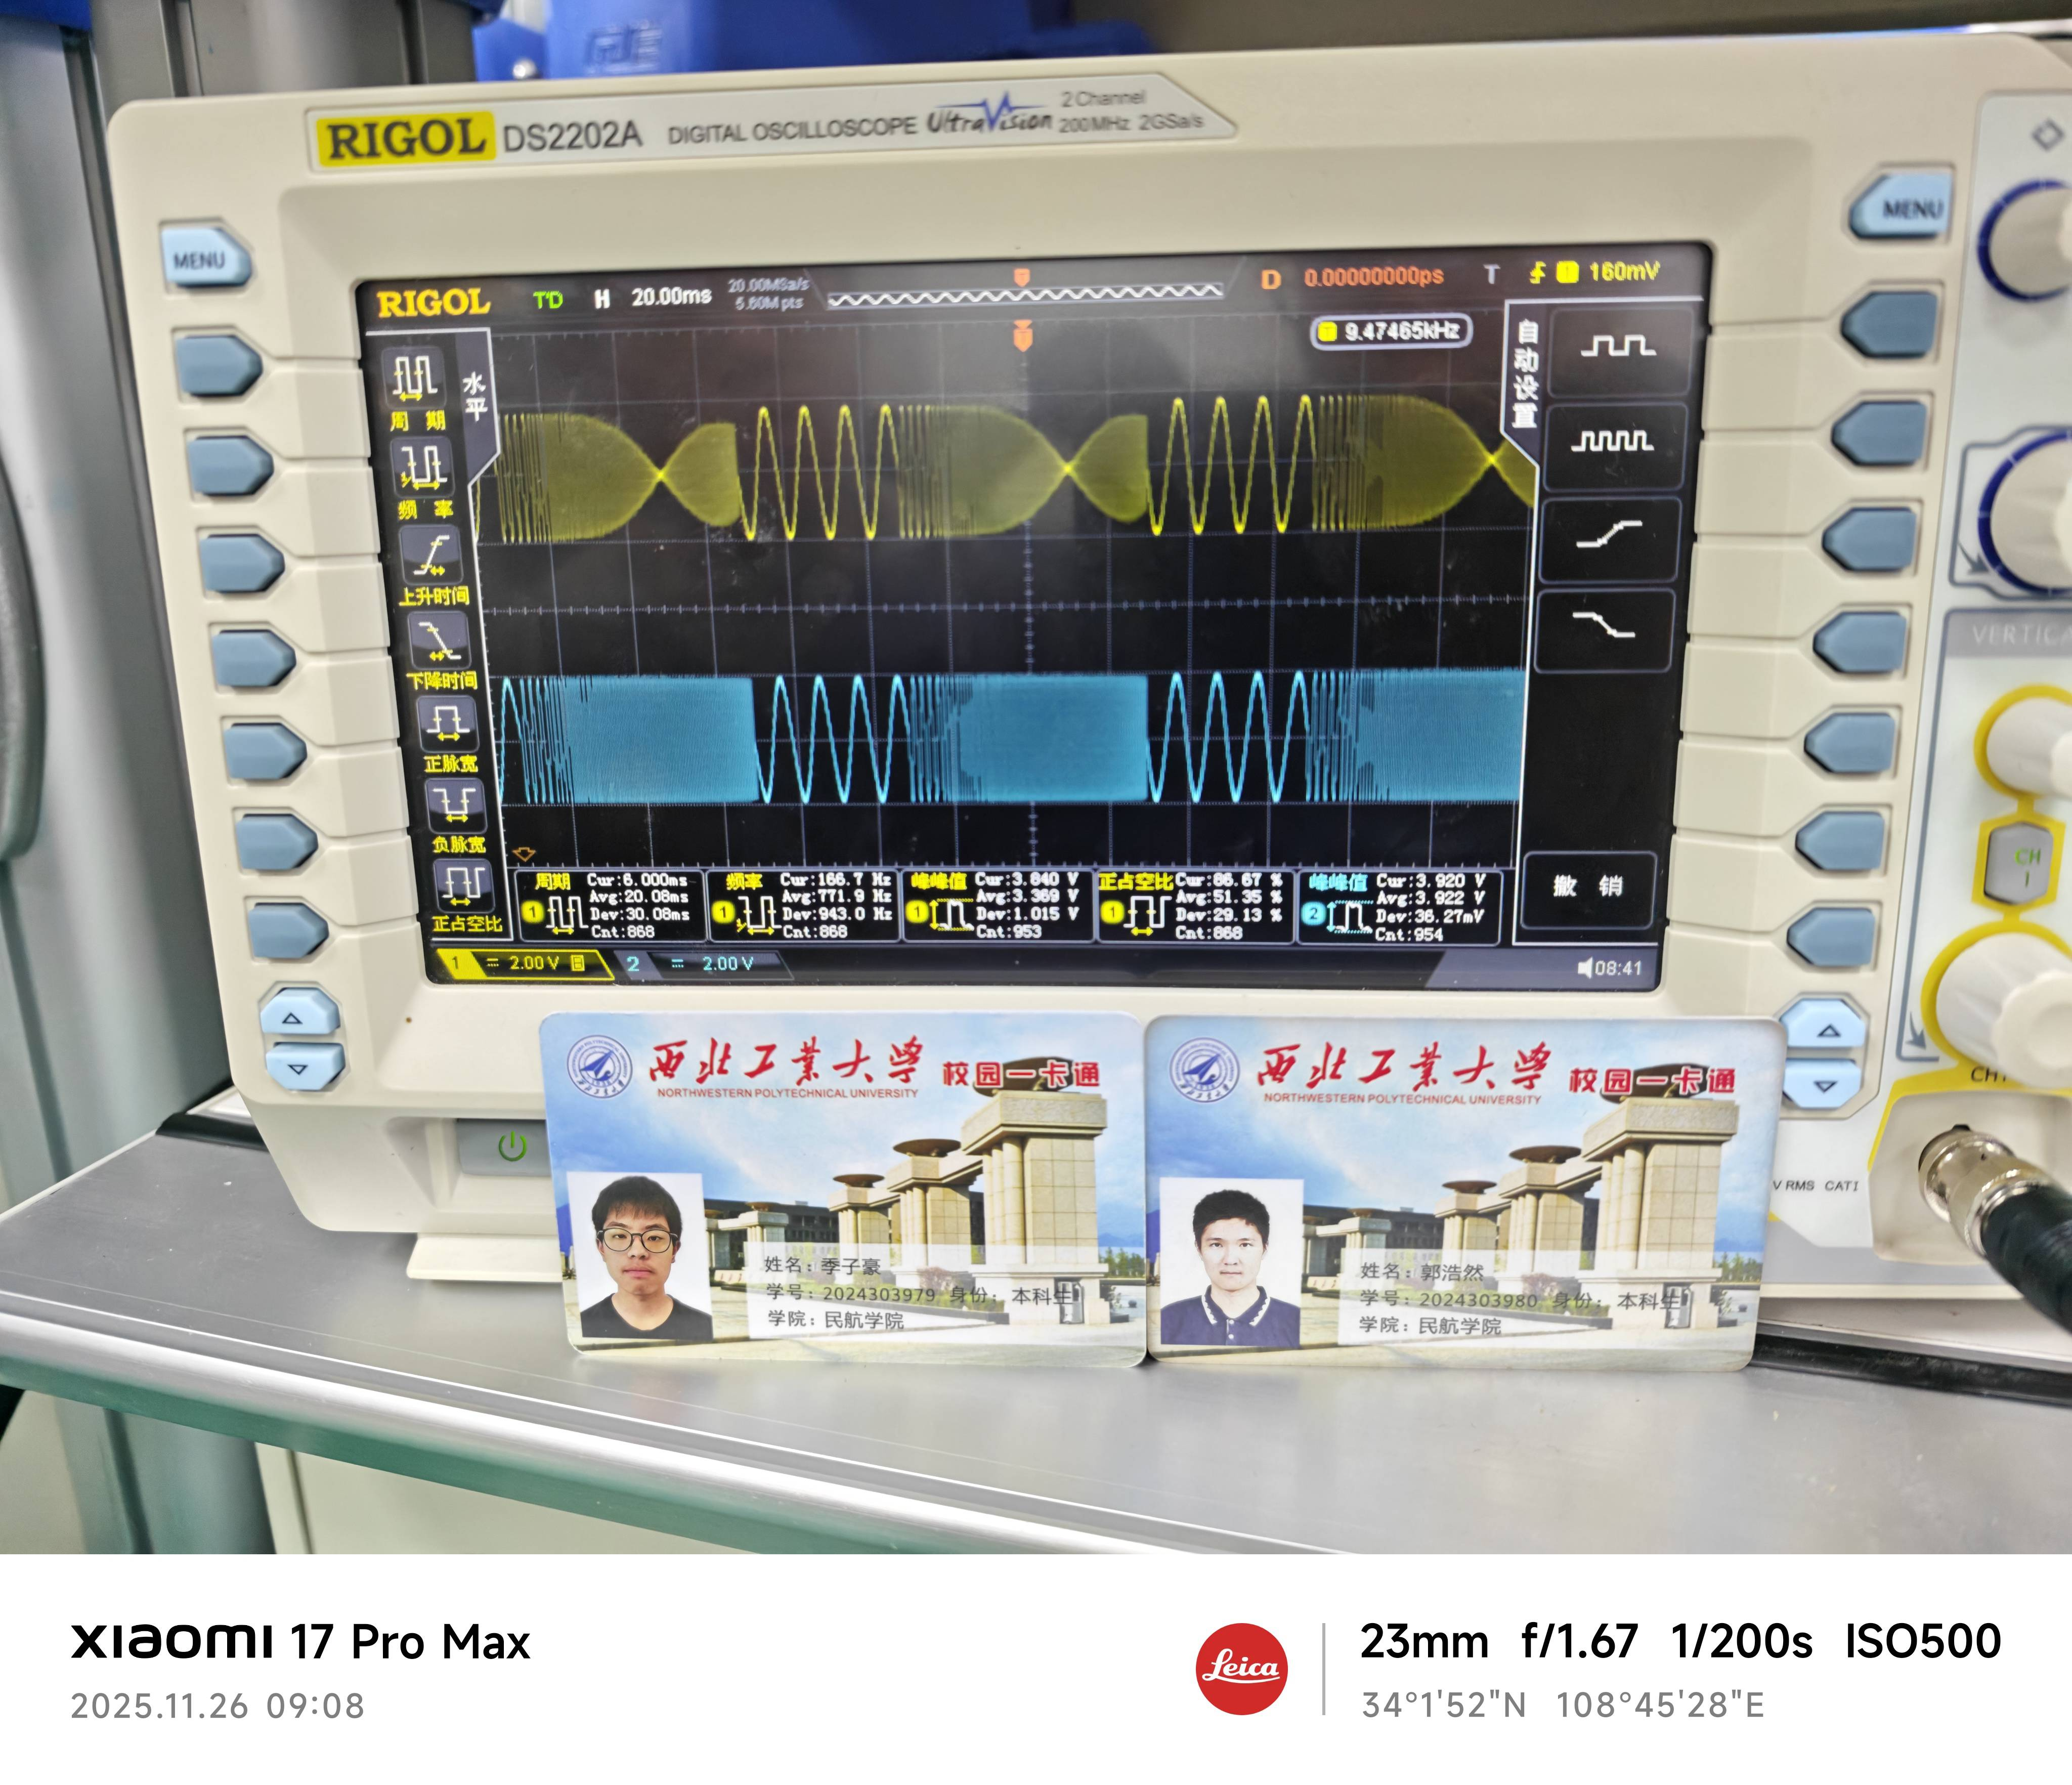
\includegraphics[width=\textwidth]{./4. frequency/figures/有源带阻.jpg}
        \caption{有源带阻扫频波形}
    \end{subfigure}
    \caption{带阻滤波器实验结果综合展示}
\end{figure}

\newpage

% ==========================================
% 第三部分：实验总结与心得
% ==========================================

\section{实验总结与心得}

\subsection{实验数据汇总}

经过对有源、无源滤波器（低通、高通、带通、带阻）的逐点测量与扫频测试，最终测得的截止频率参数汇总如表 \ref{tab:final_result} 所示。

\begin{table}[H]
    \centering
    \renewcommand{\arraystretch}{1.5}
    \setlength{\tabcolsep}{8pt}
    \begin{tabular}{|l|l|l|}
        \hline
        \textbf{类型} & \textbf{无源参数} & \textbf{有源参数} \\
        \hline
        低通 & $f_H = 18.5\,\mathrm{kHz}$ & $f_H = 16.7\,\mathrm{kHz}$ \\
        高通 & $f_L = 17.2\,\mathrm{kHz}$ & $f_L = 17.0\,\mathrm{kHz}$ \\
        \hline
        带通 & \makecell[l]{$f_L = 2.1\,\mathrm{kHz}$ \\ $f_H = 13.0\,\mathrm{kHz}$} &
               \makecell[l]{$f_L = 3.8\,\mathrm{kHz}$ \\ $f_H = 15.0\,\mathrm{kHz}$} \\
        \hline
        带阻 & \makecell[l]{$f_L = 3.6\,\mathrm{kHz}$ \\ $f_H = 85.0\,\mathrm{kHz}$} &
               \makecell[l]{$f_L = 6.5\,\mathrm{kHz}$ \\ $f_H = 45.8\,\mathrm{kHz}$} \\
        \hline
    \end{tabular}
    \caption{滤波器截止频率测量结果汇总}
    \label{tab:final_result}
\end{table}


\subsection{实验心得}

通过本次实验，我深入理解了有源与无源滤波器的基本构成及其频率响应特性。
\begin{enumerate}
    \item \textbf{测量方法的掌握}：熟练掌握了“逐点测量法”和“扫频法”两种测量幅频特性的手段。逐点法虽然繁琐，但能提供精确的量化数据，便于计算截止频率；扫频法则能直观、快速地在示波器上显示出滤波器的整体频响曲线，便于定性分析。
    \item \textbf{理论与实践的结合}：实验中观察到的幅频特性曲线与理论分析基本一致。例如，低通滤波器在高频段的衰减、带通滤波器的选频特性等都在实验中得到了验证。同时，也观察到了实际元器件参数误差对截止频率的影响，这提示我们在工程实践中需要考虑元器件的容差。
    \item \textbf{有源与无源的对比}：通过对比发现，有源滤波器由于引入了运放，具有一定的信号放大能力（通带增益可能大于1），且负载效应较小；而无源滤波器结构简单，但信号经过后会有一定的衰减。
\end{enumerate}

% ===================================================================
% 第五章：抽样定理和信号的恢复 (Origin: 5. sample)
% ===================================================================
\chapter{抽样定理和信号的恢复}

% ================= 第一部分：实验目的 =================
\section{实验目的}
\begin{enumerate}
    \item 观察离散信号频谱，了解其频谱特点。
    \item 验证抽样定理并恢复原信号。
    \item 初步了解 MATLAB 软件的基本使用。
\end{enumerate}

% ================= 第二部分：实验器材 =================
\section{实验器材}
\begin{itemize}
    \item 双踪示波器 \hfill 1台
    \item 信号源及频率计模块 (S2) \hfill 1块
    \item 抽样定理及滤波器模块 (S3) \hfill 1块
    \item 数字信号处理模块 (S4) \hfill 1块 % 根据PPT截图补充
\end{itemize}

% ================= 第三部分：实验原理  =================
\section{实验原理}
\subsection{信号的抽样}
离散信号可以从对连续信号的抽样获得。抽样信号 $F_s(t)$ 可表示为连续信号 $F(t)$ 与周期性矩形窄脉冲 $S(t)$ 的乘积：
\begin{equation}
    F_s(t) = F(t) \cdot S(t)
\end{equation}
其中，$S(t)$ 的周期为 $T_s$（抽样间隔），抽样频率为 $f_s = 1/T_s$。抽样过程的波形如图 \ref{fig:sampling_process} 所示。
\begin{figure}[htbp]
    \centering
    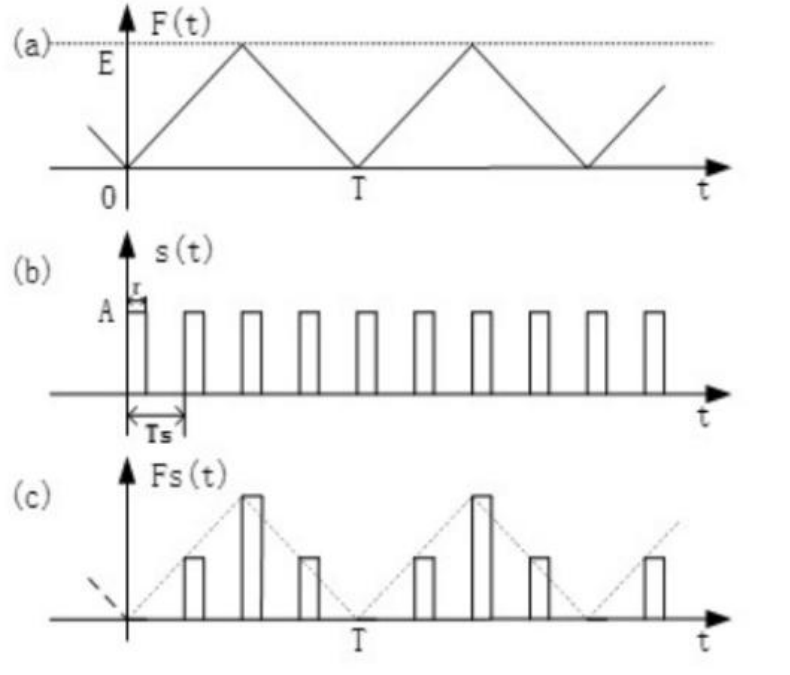
\includegraphics[width=0.4\textwidth]{./5. sample/figures/fig5-1.png} 
    \caption{连续信号抽样过程波形图 ($F(t) \to S(t) \to F_s(t)$)}
    \label{fig:sampling_process}
\end{figure}
\subsection{抽样定理与信号恢复}
\textbf{抽样定理}指出：若要从抽样信号中无失真地恢复出原信号，抽样频率 $f_s$ 必须大于等于原信号最高频率分量 $f_m$ 的两倍，即满足奈奎斯特判据：
\begin{equation}
    f_s \geq 2B_f \quad (\text{其中 } B_f \text{ 为原信号带宽})
\end{equation}
\begin{itemize}
    \item 若 $f_s \geq 2B_f$，抽样信号的频谱是原信号频谱的周期性延拓，且各频谱分量不重叠。通过一个截止频率 $f_c$ 满足 $f_m \leq f_c \leq f_s - f_m$ 的低通滤波器，即可滤出原信号频谱，恢复原波形。
    \item 若 $f_s < 2B_f$，频谱发生混叠（Aliasing），无法通过低通滤波器恢复原信号。
\end{itemize}
工程实际中，为了减小滤波器设计难度并减轻失真，通常采用过采样，即 $f_s > 2.56 f_m$。
\subsection{S3 模块的抽样功能}
本实验使用 S3 模块进行自然抽样及恢复，流程如图 \ref{fig:system_flow} 所示。模块提供两种抽样方式：
\begin{enumerate}
    \item \textbf{同步抽样}：抽样时钟与连续信号由同一晶振源产生，时钟严格对齐，便于观察稳定的抽样波形。
    \item \textbf{异步抽样}：连续信号与抽样时钟由不同源产生，模拟实际通信中收发端不同步的情况。
\end{enumerate}
\begin{figure}[htbp]
    \centering
    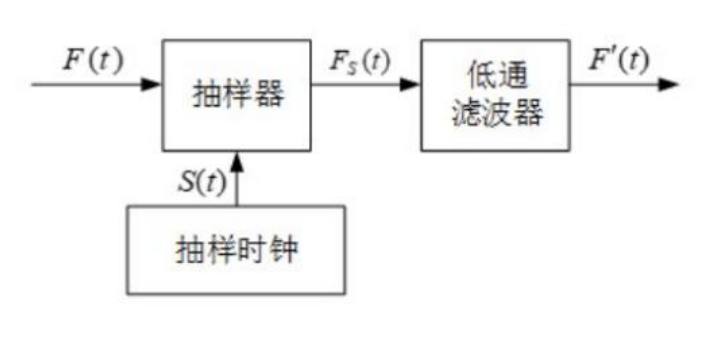
\includegraphics[width=0.5\textwidth]{./5. sample/figures/fig5-5.png}
    \caption{信号自然抽样及恢复实验流程图}
    \label{fig:system_flow}
\end{figure}

% ================= 四、实验步骤 =================
\section{实验步骤}

\subsection{任务：自然抽样及恢复}

\subsubsection{观察抽样信号波形 (异步)}
\begin{enumerate}
    \item 将 S2 模块的扫频开关 S3 置为“OFF”。调节模拟信号源，使 P2 处输出频率为 \SI{500}{Hz}、幅度为 \SI{2}{V} 的正弦波。
    \item 连接 S2 模块输出端 P2 与 S3 模块连续信号输入点 P17。
    \item 将开关 S2 拨至“异步”。示波器 CH1 接原始信号 (TP2)，CH2 接抽样信号 (TP20)。
    \item 调节电位器 W1，使抽样频率分别为 \SI{1}{kHz}, \SI{2}{kHz}, \SI{4}{kHz}, \SI{8}{kHz}。观察并记录波形。
    \item \textbf{注意}：调节 W1 时，需用示波器测量 TP21 (开关信号) 的频率以确保准确。
\end{enumerate}

\subsubsection{观察抽样信号波形 (同步)}
\begin{enumerate}
    \item 保持 P2 与 P17 的连接。连接 S2 模块时钟输出 P5 与 S3 模块外部开关信号输入点 P18。
    \item 将开关 S2 拨至“同步”。示波器 CH1 接原始信号 (TP2)，CH2 接抽样信号 (TP20)。
    \item 调节 S2 模块的时钟频率设置按钮 S7，使抽样频率分别为 \SI{1}{kHz}, \SI{2}{kHz}, \SI{4}{kHz}, \SI{8}{kHz}。观察并记录波形。
\end{enumerate}

\subsubsection{验证抽样定理与信号恢复}
\begin{enumerate}
    \item 连接 S3 模块的 P20 和 P19 (将抽样信号送入低通滤波器)。
    \item 示波器 CH1 接原始抽样信号 (TP17)，CH2 接恢复信号输出点 (TP22)。
    \item 改变抽样时钟频率，对比观察信号恢复情况，验证奈奎斯特抽样定理。
\end{enumerate}

% ================= 五、实验数据与分析 =================
\section{实验数据与分析}

\subsection{信号的抽样波形记录}

\subsubsection{同步抽样波形}
输入信号：正弦波，幅度 \SI{1.920}{V}，频率 \SI{1}{kHz}。
不同抽样频率下的波形如图 \ref{fig:sync_sampling} 所示，数据记录如表 \ref{tab:sync_data}。

% --- 表格排版：三线表 ---
\begin{table}[H]
    \centering
    \caption{同步抽样实验数据记录}
    \label{tab:sync_data}
    \begin{tabular}{cccc}
        \toprule
        \textbf{输入信号} & \textbf{抽样频率 ($f_s$)} & \textbf{抽样信号峰峰值 ($V_{pp}$)} & \textbf{波形描述} \\
        \midrule
        \multirow{4}{*}{\shortstack{1.920V \\ 1kHz}} 
        & \SI{1}{kHz} & \SI{1.610}{V} & 临界采样，波形失真较大 \\
        & \SI{2}{kHz} & \SI{2.040}{V} & 过采样，波形包络清晰 \\
        & \SI{4}{kHz} & \SI{2.094}{V} & 抽样点密集，拟合度高 \\
        & \SI{8}{kHz} & \SI{2.155}{V} & 抽样点极密，接近原波形 \\
        \bottomrule
    \end{tabular}
\end{table}

% --- 图片排版：2x2 网格 ---
\begin{figure}[htbp]
    \centering
    \begin{subfigure}[b]{0.45\textwidth}
        \centering
        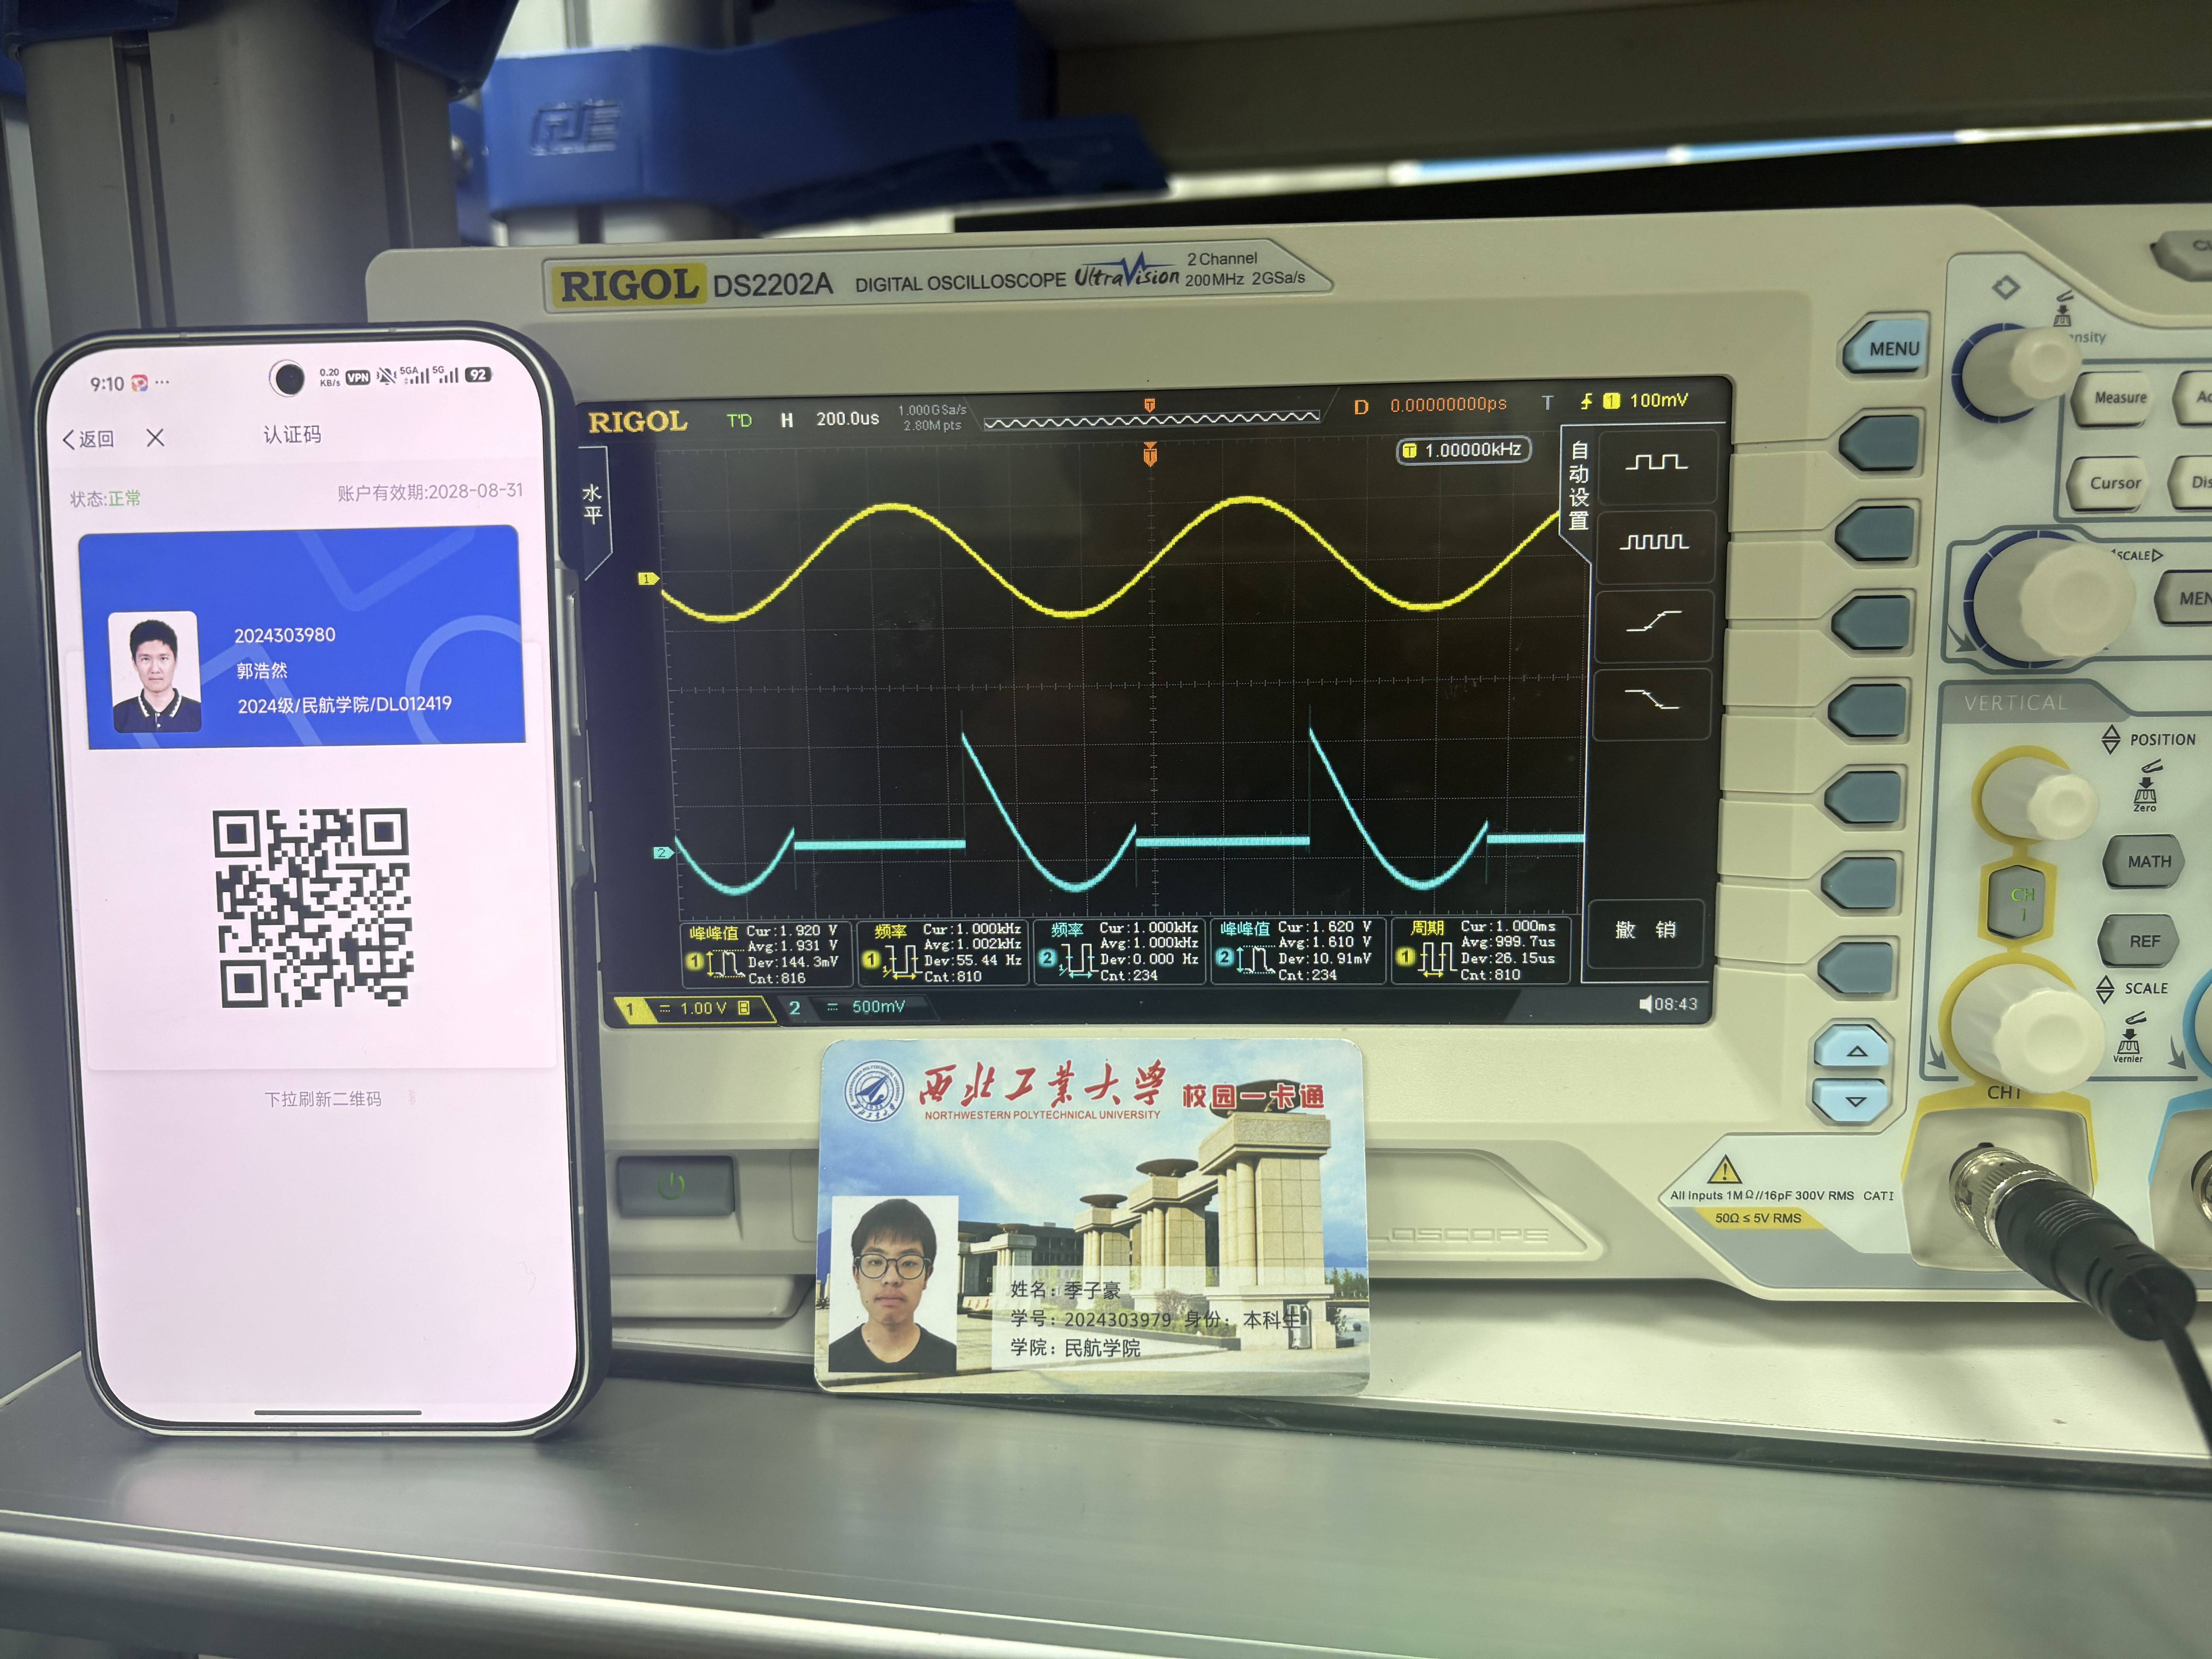
\includegraphics[width=\textwidth]{./5. sample/figures/同步1k.jpg} 
        \caption{$f_s = \SI{1}{kHz}$}
    \end{subfigure}
    \hfill
    \begin{subfigure}[b]{0.45\textwidth}
        \centering
        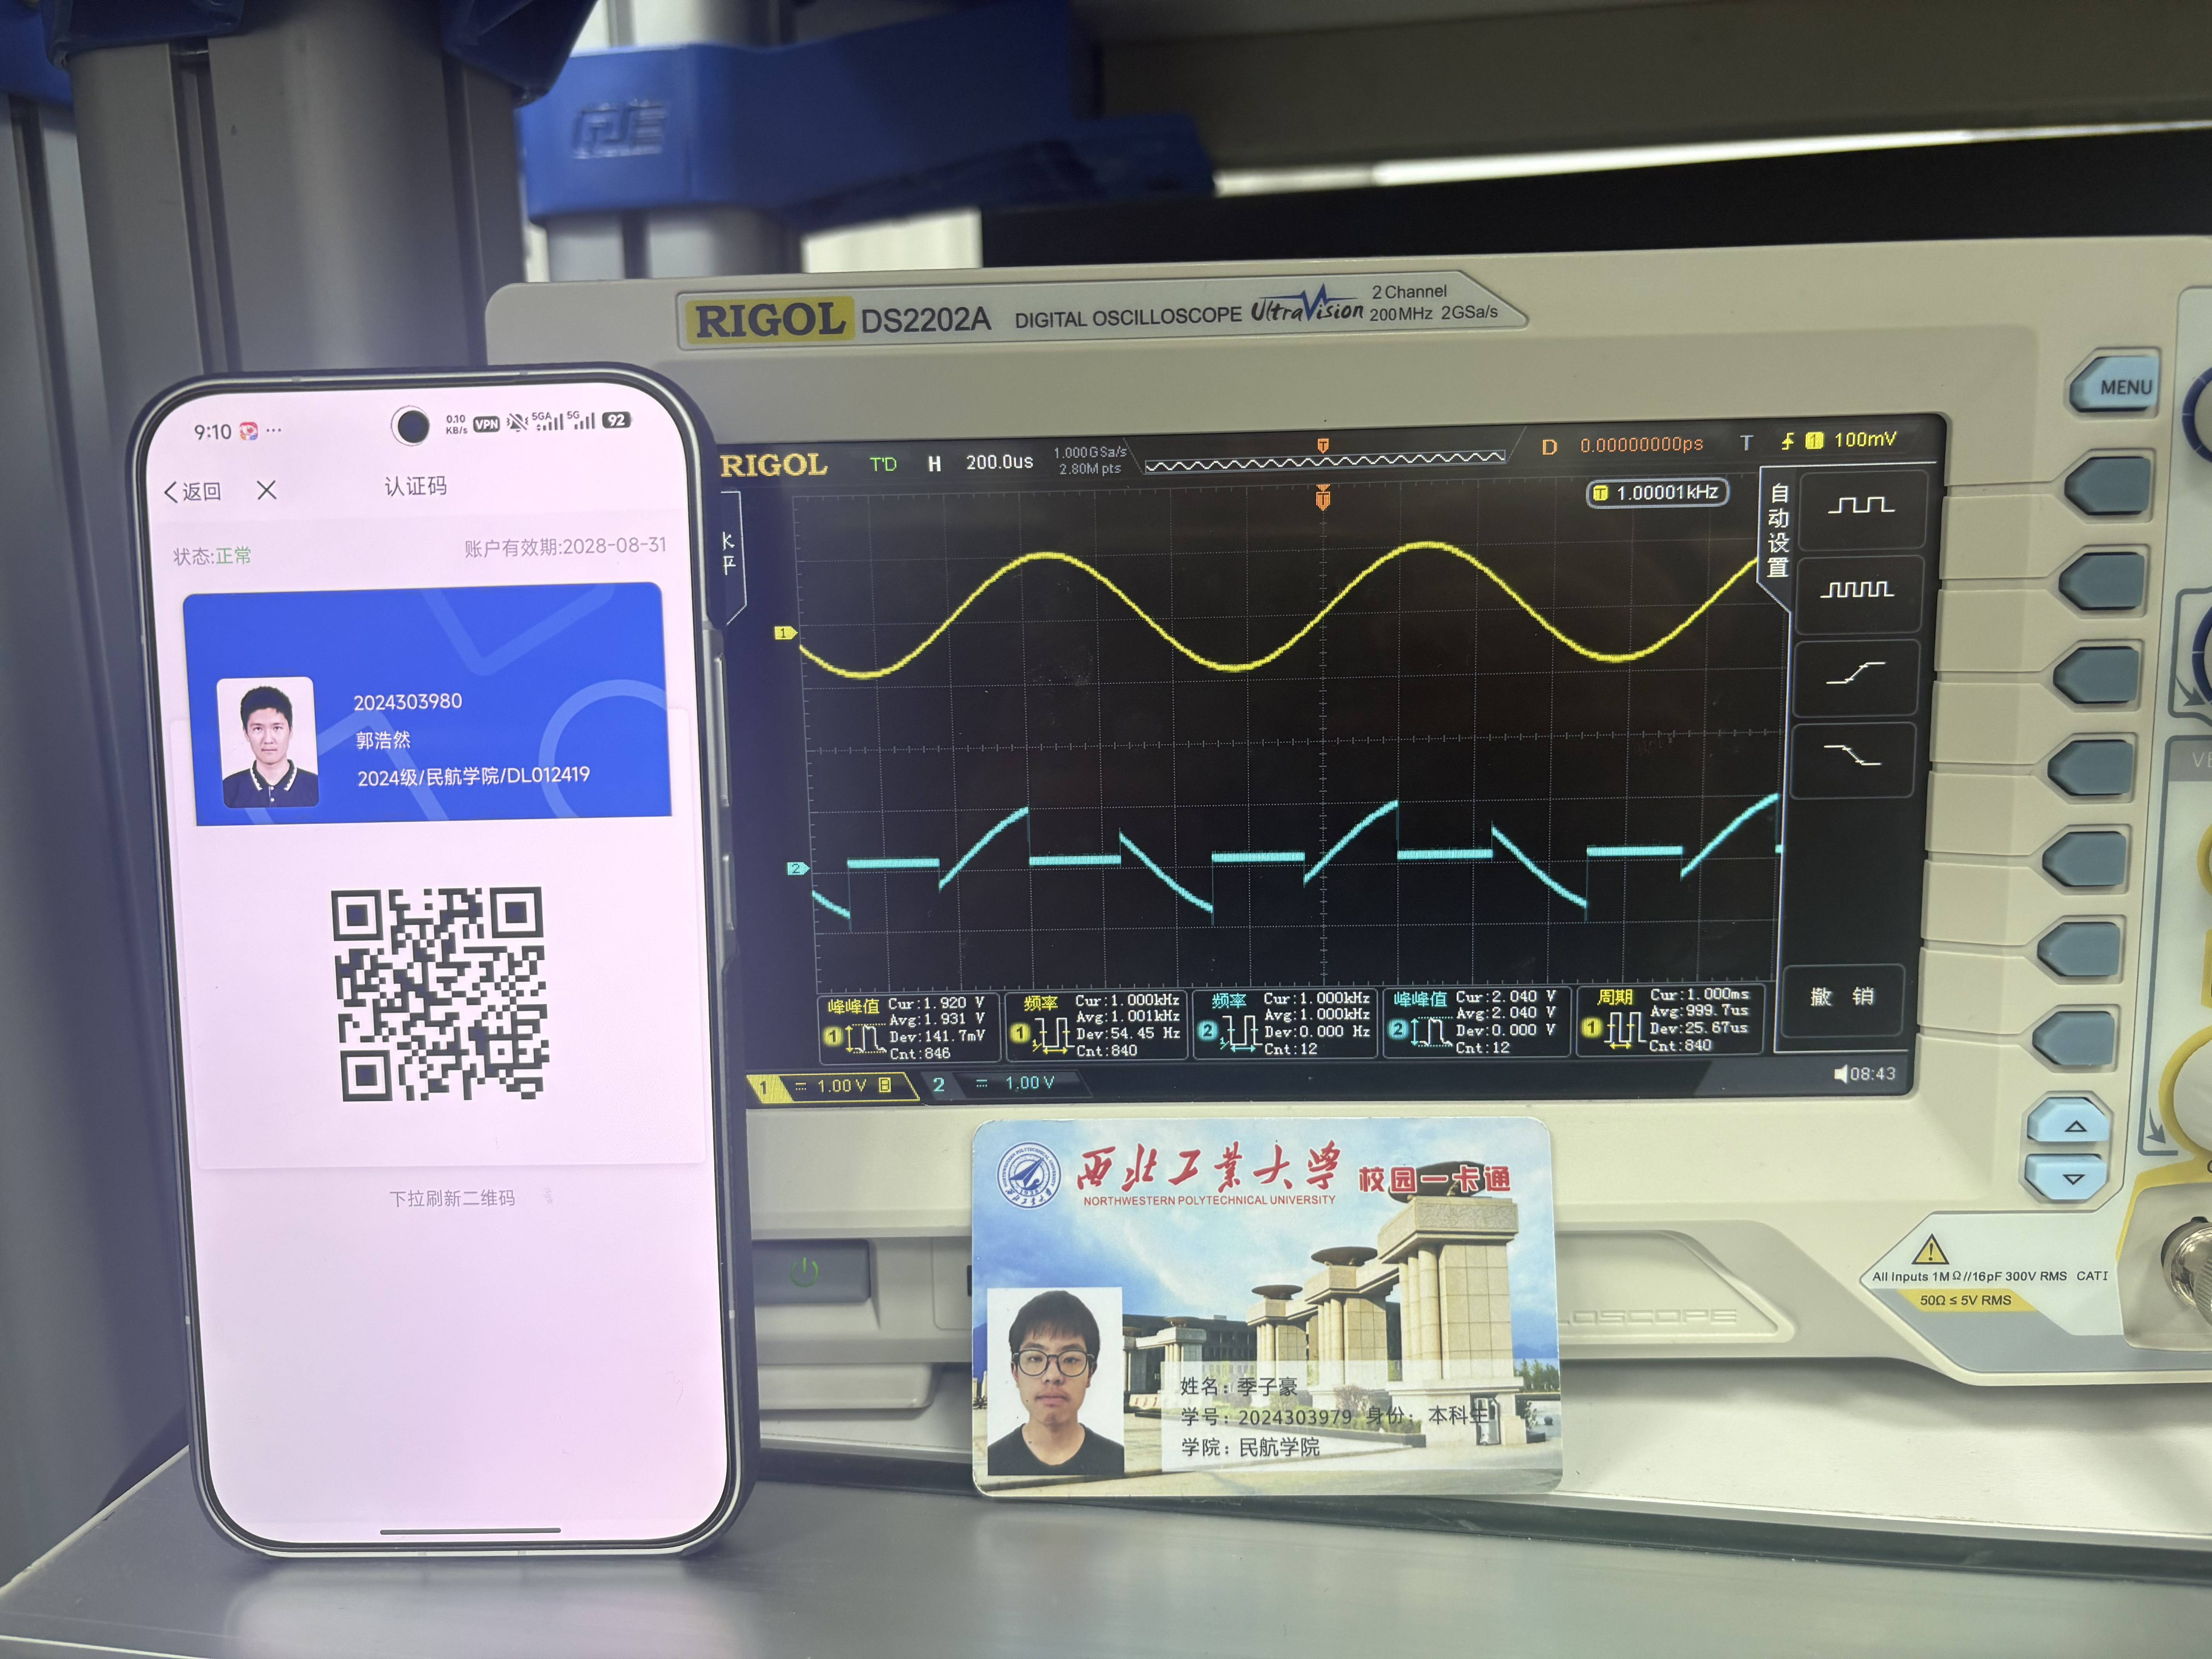
\includegraphics[width=\textwidth]{./5. sample/figures/同步2k.jpg}
        \caption{$f_s = \SI{2}{kHz}$}
    \end{subfigure}
    
    \vspace{0.5cm} % 上下两行间距
    
    \begin{subfigure}[b]{0.45\textwidth}
        \centering
        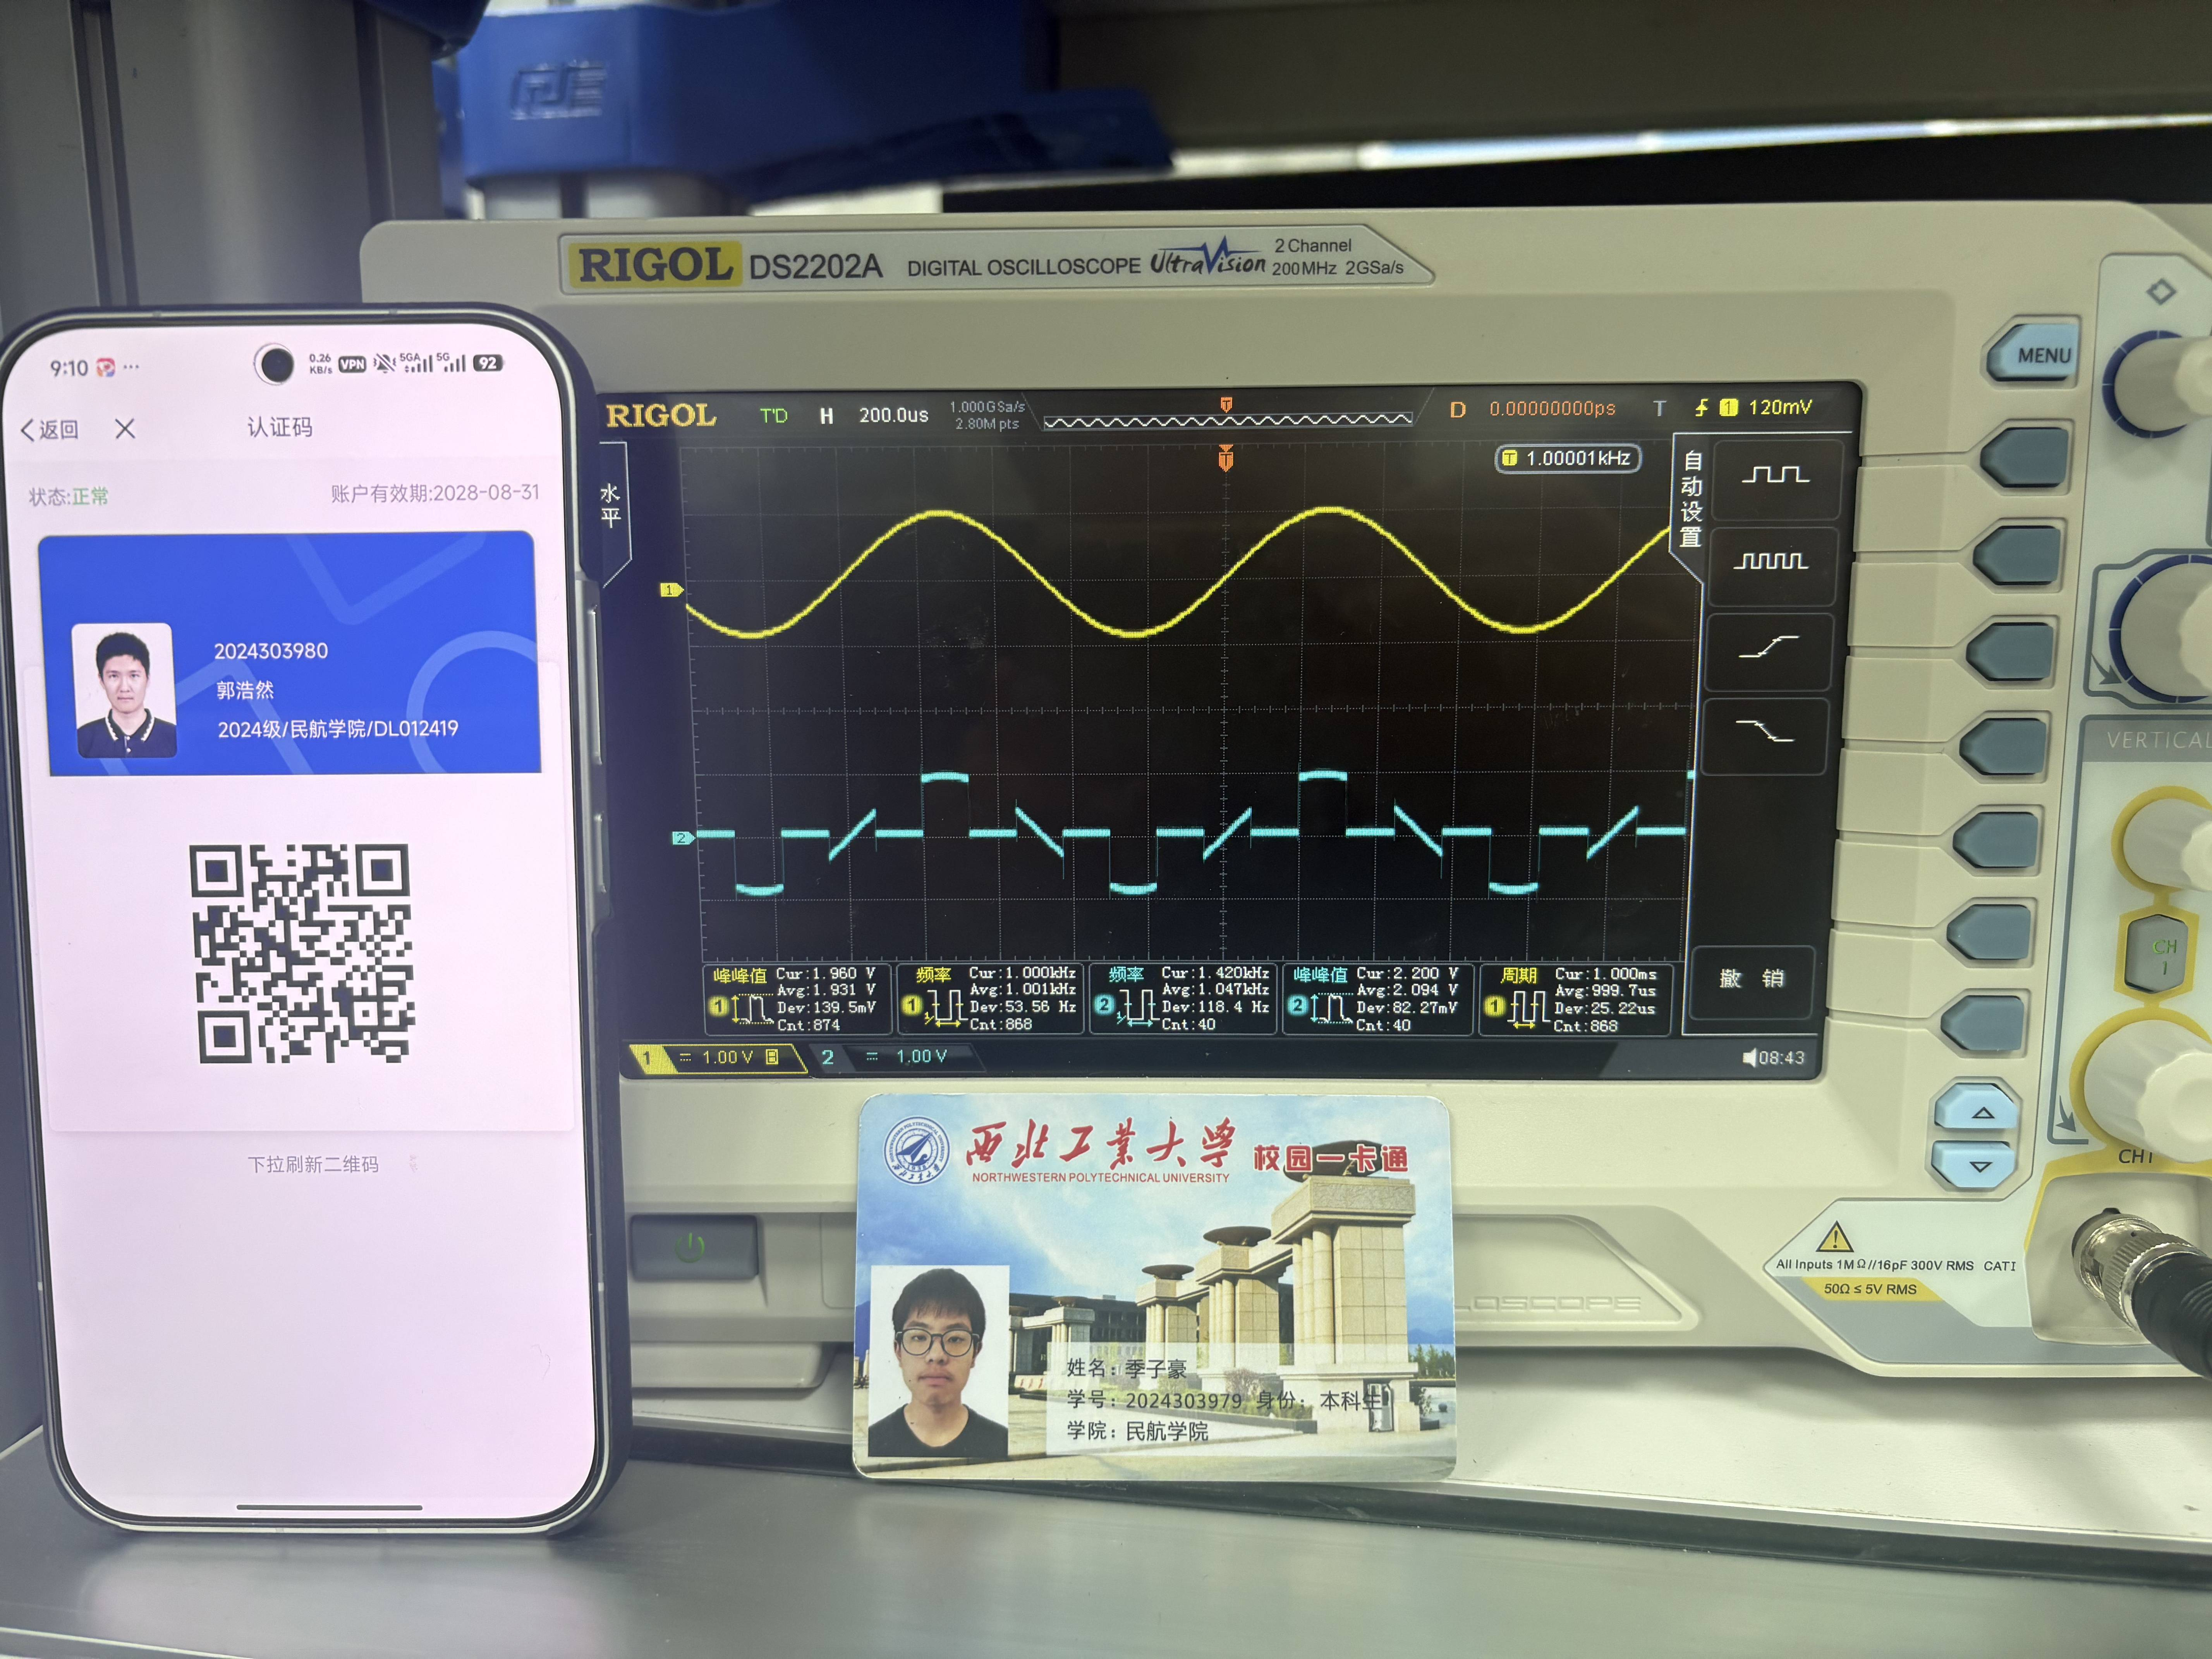
\includegraphics[width=\textwidth]{./5. sample/figures/同步4k.jpg}
        \caption{$f_s = \SI{4}{kHz}$}
    \end{subfigure}
    \hfill
    \begin{subfigure}[b]{0.45\textwidth}
        \centering
        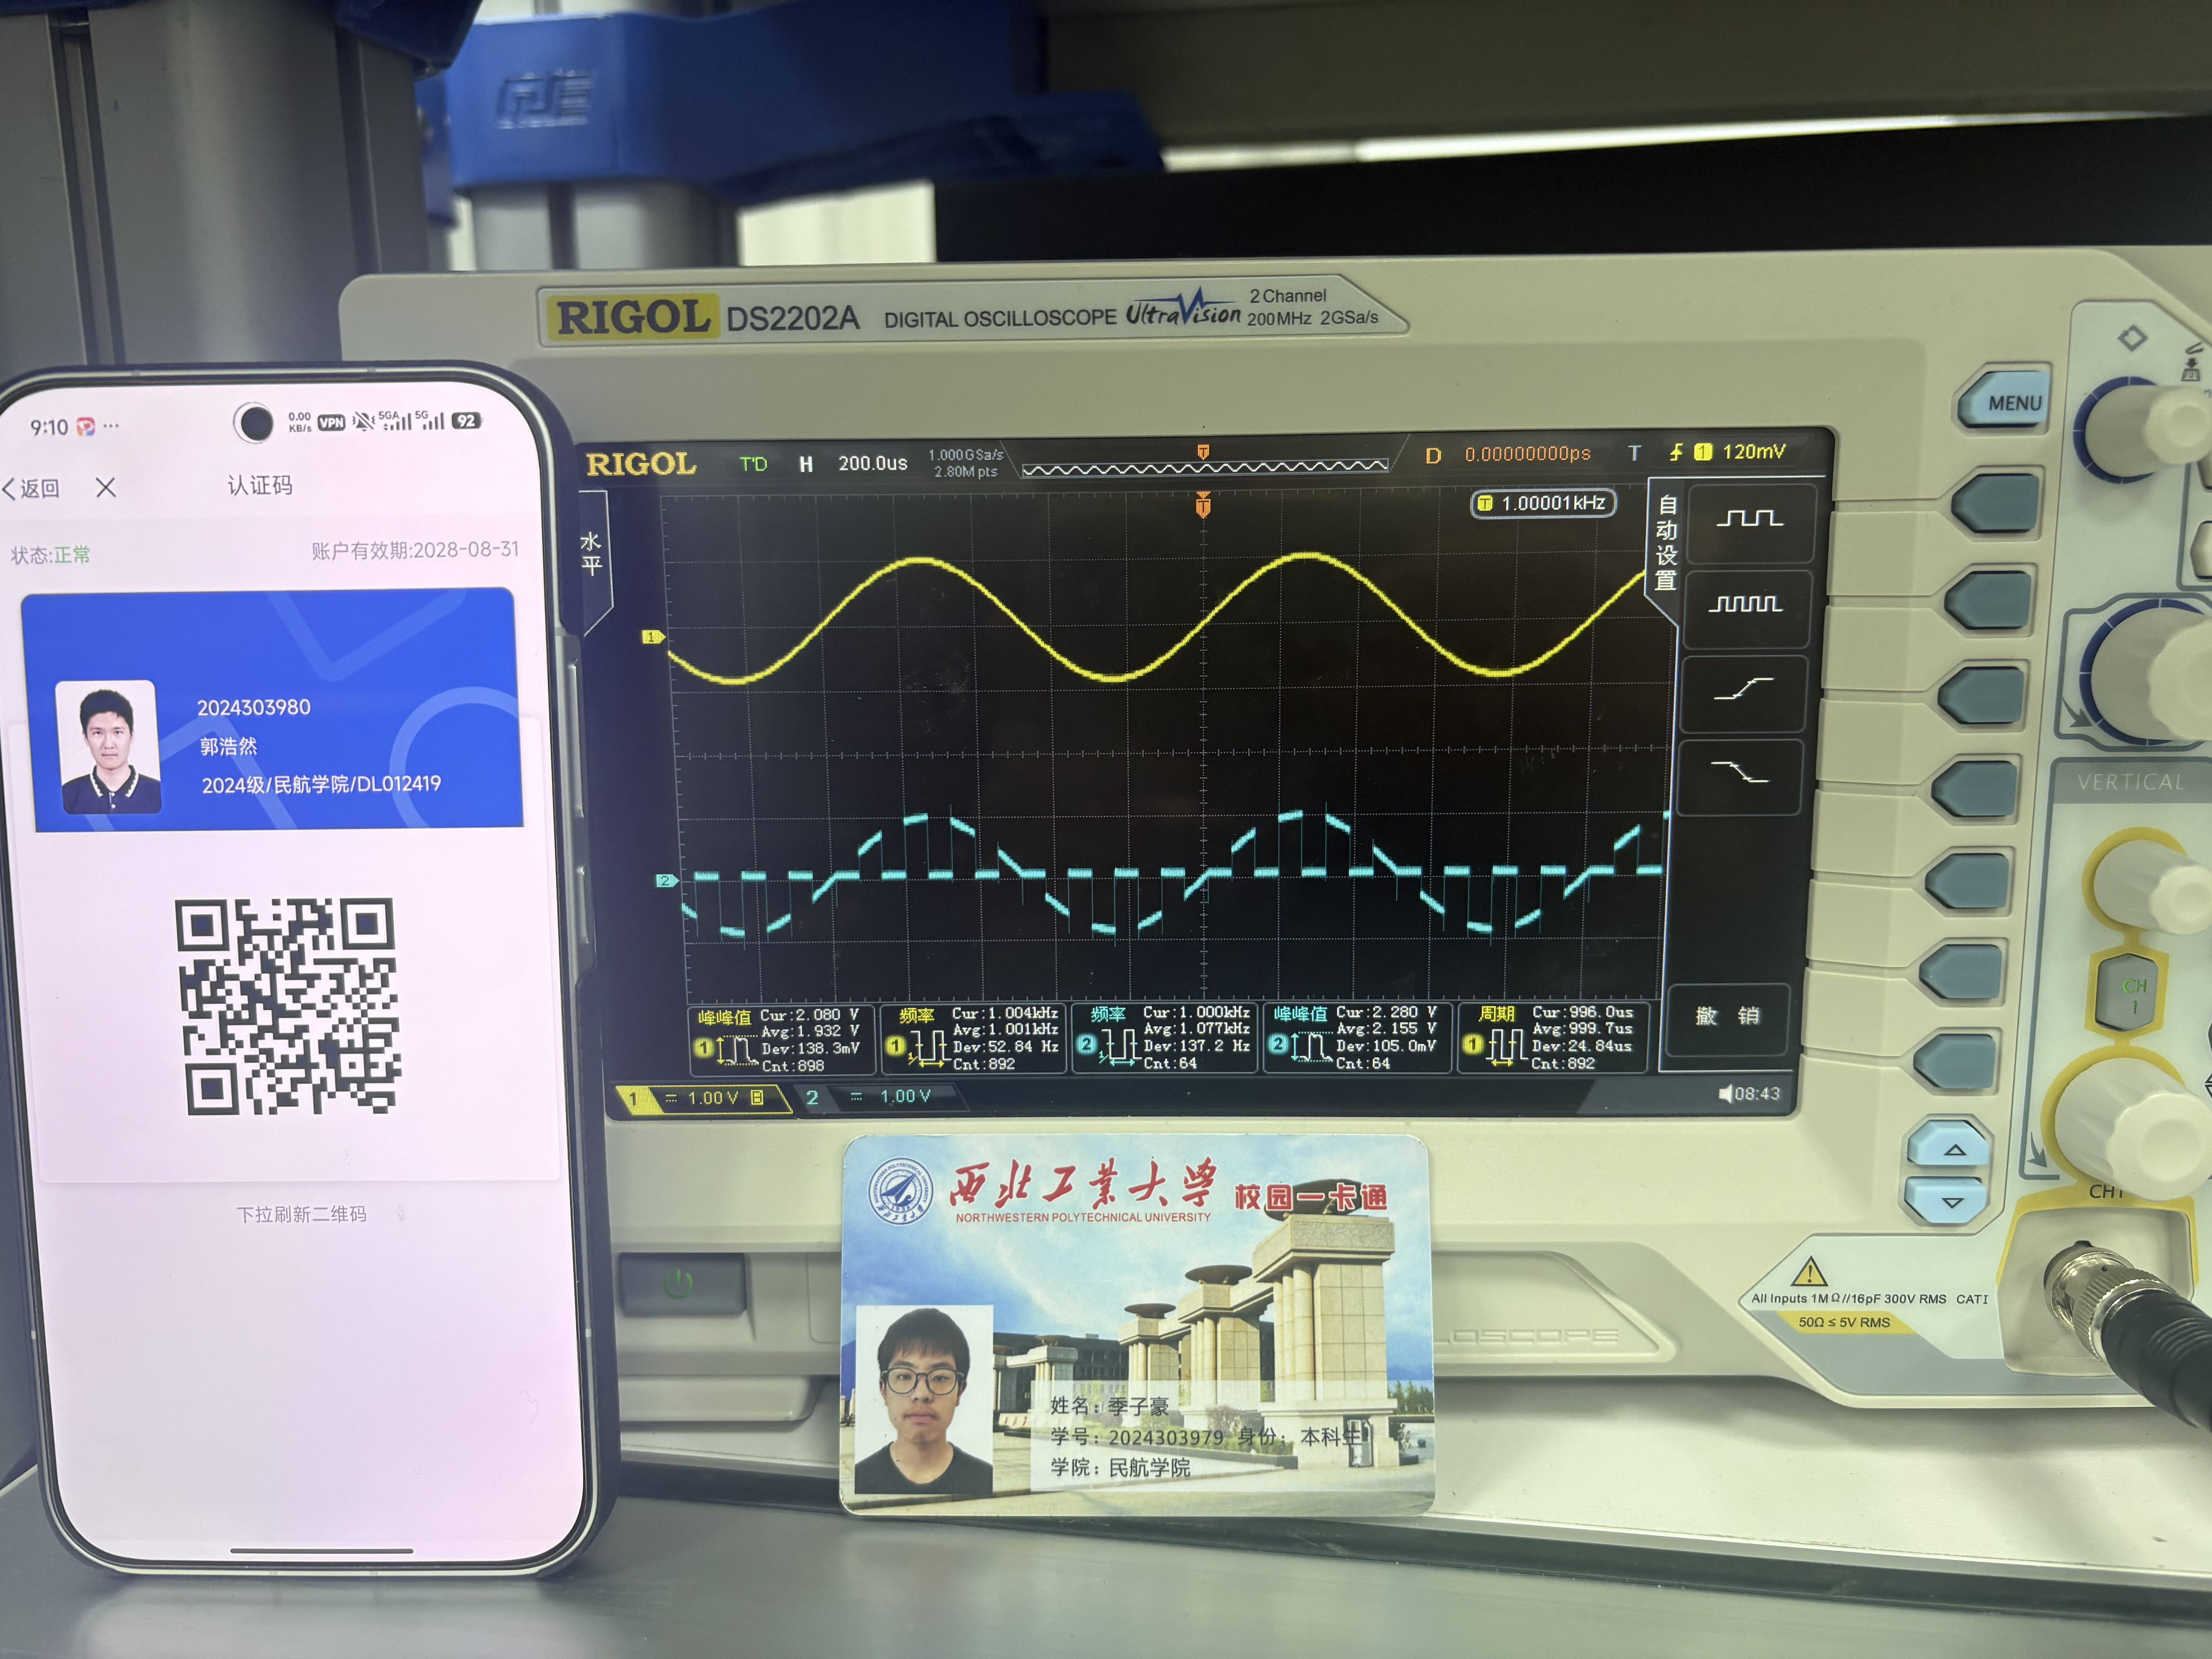
\includegraphics[width=\textwidth]{./5. sample/figures/同步8k.jpg}
        \caption{$f_s = \SI{8}{kHz}$}
    \end{subfigure}
    \caption{同步抽样波形观测 (蓝色：抽样信号，黄色：输入信号)}
    \label{fig:sync_sampling}
\end{figure}


\subsubsection{异步抽样波形}
输入信号同上。不同抽样频率下的波形如图 \ref{fig:async_sampling} 所示，数据记录如表 \ref{tab:async_data}。

% --- 图片排版：2x2 网格 ---
\begin{figure}[htbp]
    \centering
    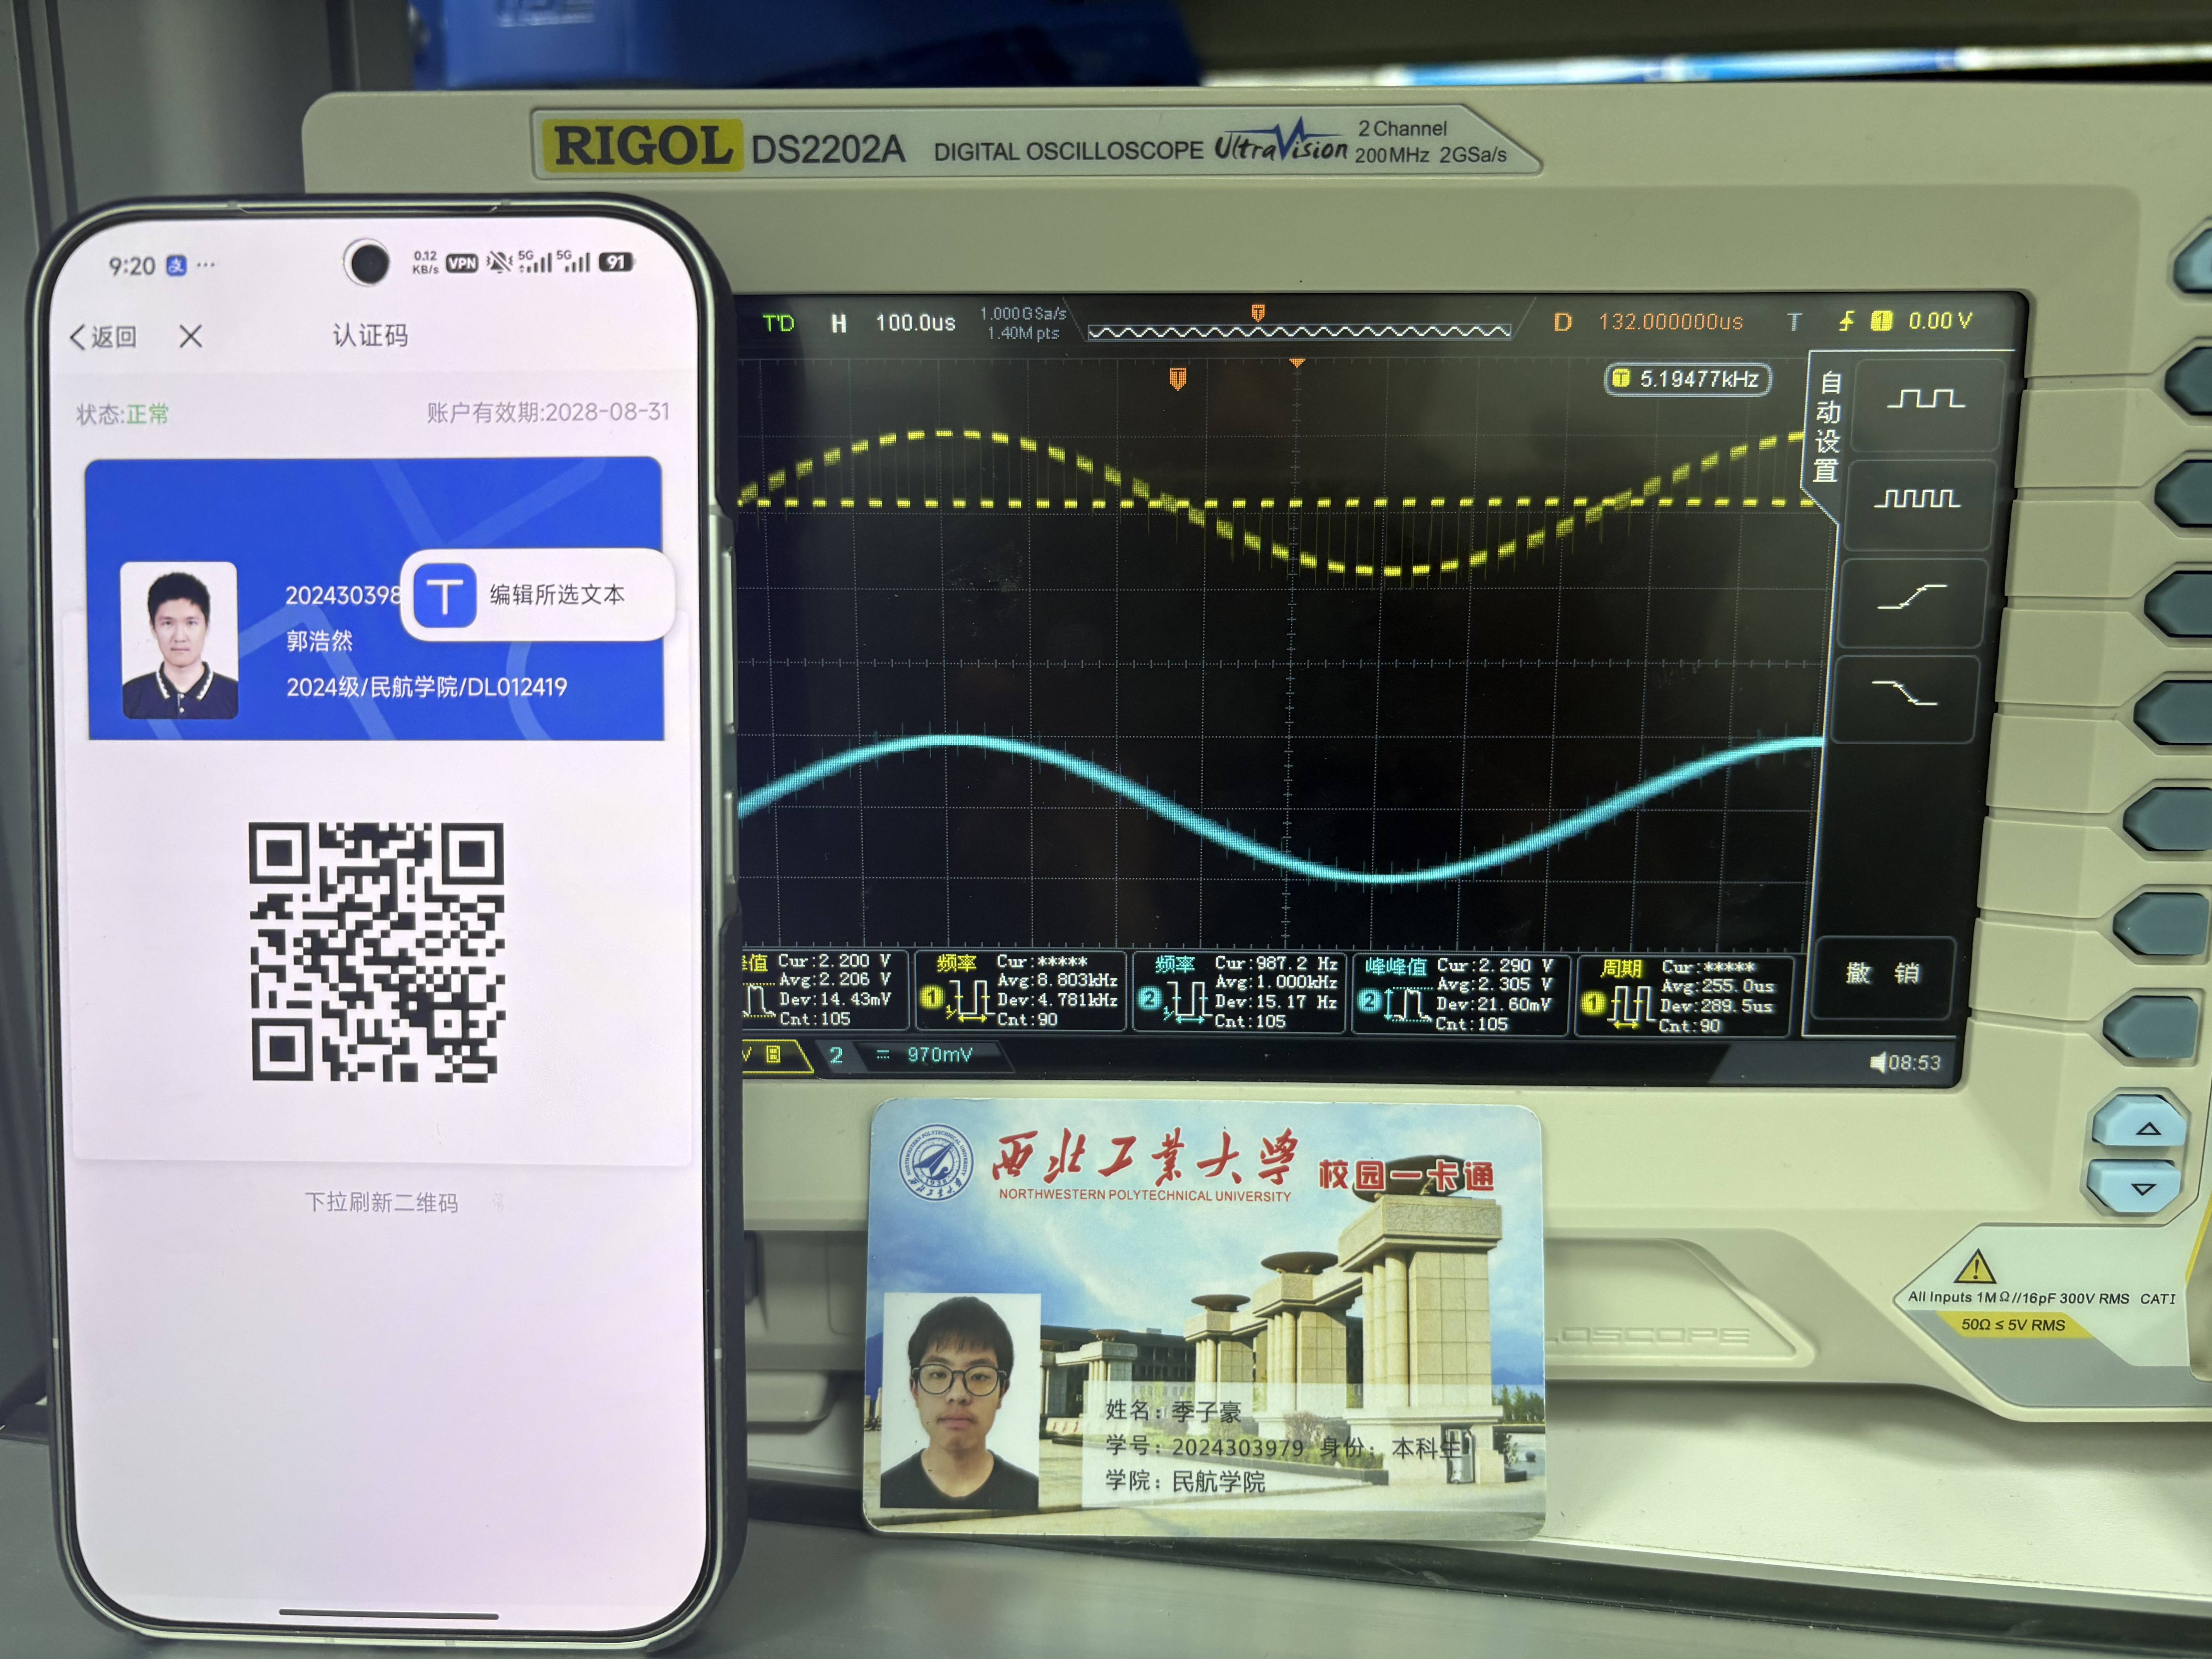
\includegraphics[width=0.6\textwidth]{./5. sample/figures/异步.jpg}
    \caption{异步抽样波形观测}
    \label{fig:async_sampling}
\end{figure}

\begin{table}[H]
    \centering
    \caption{异步抽样实验数据记录}
    \label{tab:async_data}
    \begin{tabular}{ccc}
        \toprule
        \textbf{输入信号} & \textbf{抽样频率 ($f_s$)} & \textbf{抽样信号峰峰值 ($V_{pp}$)} \\
        \midrule
        \multirow{1}{*}{2.305V 1kHz} 
        & \SI{8}{kHz} & \SI{2.206}{V} \\
        \bottomrule
    \end{tabular}
\end{table}

\subsection{信号恢复实验}
输入信号频率为 \SI{1}{kHz}，验证抽样定理。恢复波形如图 \ref{fig:recovery} 所示。


\begin{table}[H]
    \centering
    \caption{信号恢复实验结果分析 ($f_{in} = \SI{1.7}{kHz}$)}
    \label{tab:recovery_data}
    \begin{tabular}{cccl}
        \toprule
        \textbf{抽样频率} & \textbf{理论判据 ($2f_{in}$)} & \textbf{状态} & \textbf{恢复结果 (TP22)} \\
        \midrule
        \SI{1}{kHz} & \multirow{4}{*}{\SI{2}{kHz}} & $f_s < 2f_{in}$ & 严重失真，混叠 \\
        \SI{2}{kHz} & & $f_s = 2f_{in}$ & 恰好恢复 \\
        \SI{4}{kHz} & & $f_s > 2f_{in}$ & 能够恢复正弦波 \\
        \SI{8}{kHz} & & $f_s \gg 2f_{in}$ & 完美恢复，波形光滑 \\
        \bottomrule
    \end{tabular}
\end{table}

% --- 图片排版：2x2 网格 ---
\begin{figure}[H]
    \centering
    \begin{subfigure}[b]{0.45\textwidth}
        \centering
        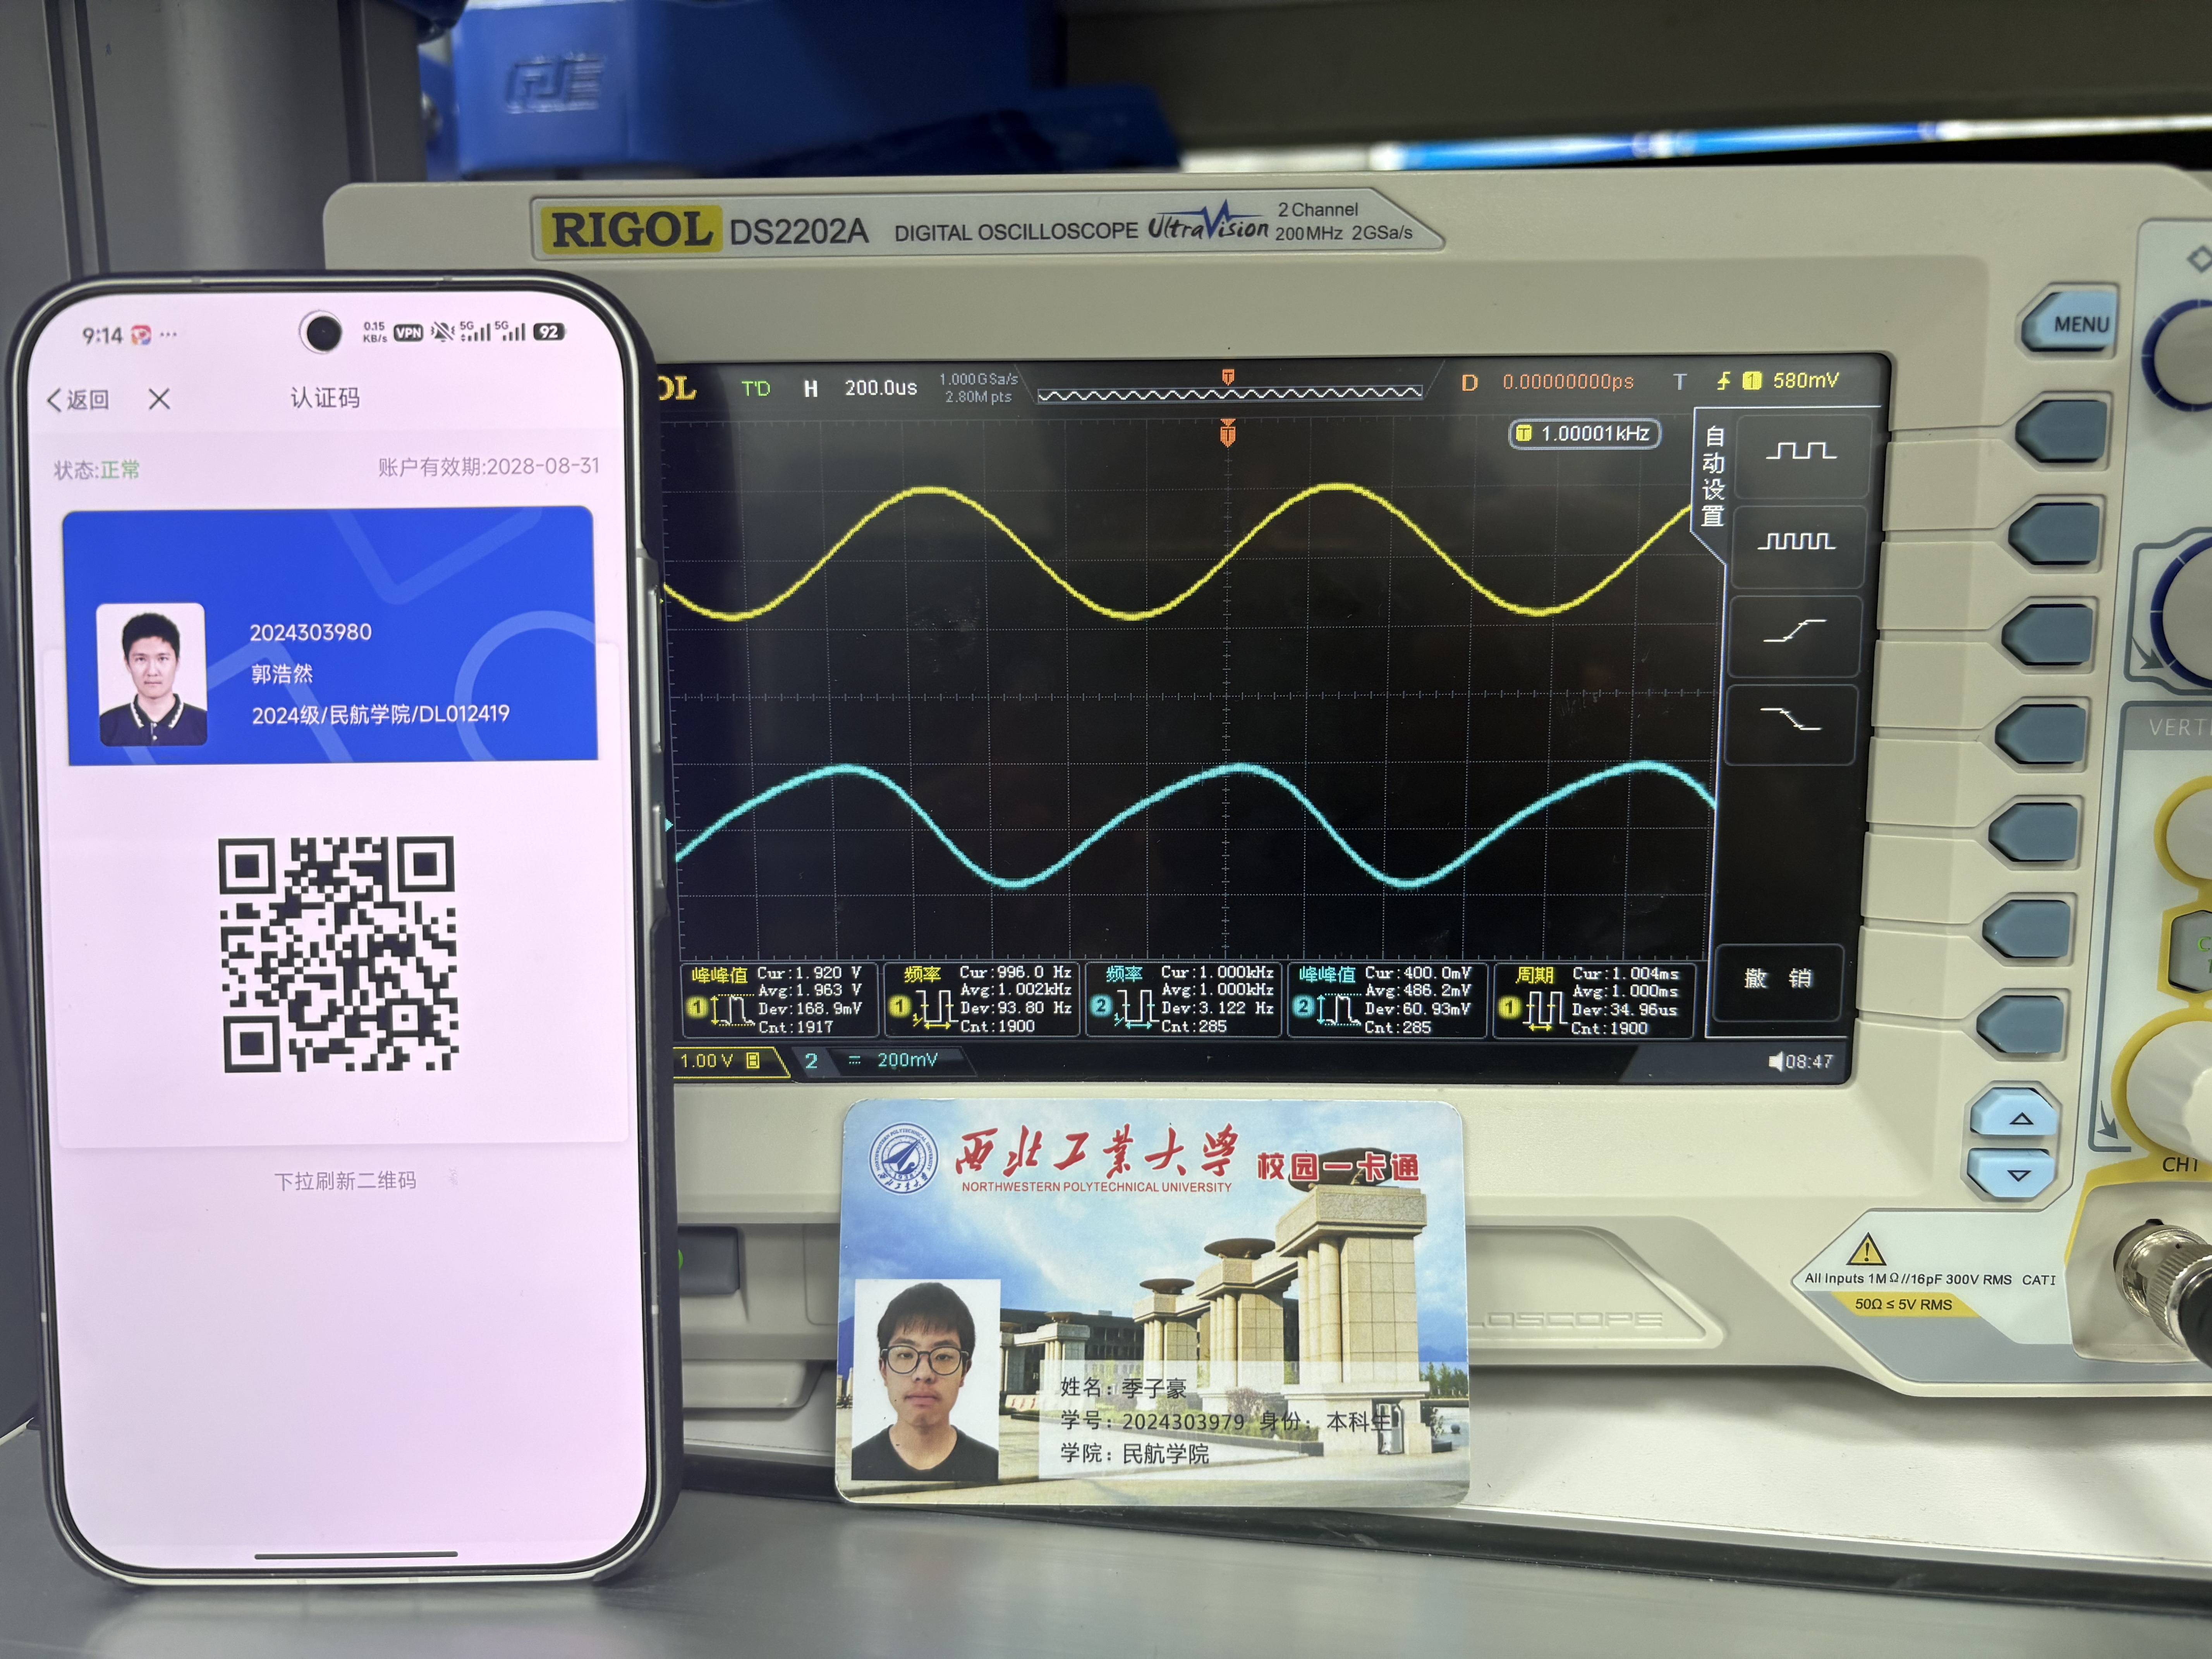
\includegraphics[width=\textwidth]{./5. sample/figures/恢复1k.jpg} 
        \caption{$f_s = \SI{1}{kHz}$}
    \end{subfigure}
    \hfill
    \begin{subfigure}[b]{0.45\textwidth}
        \centering
        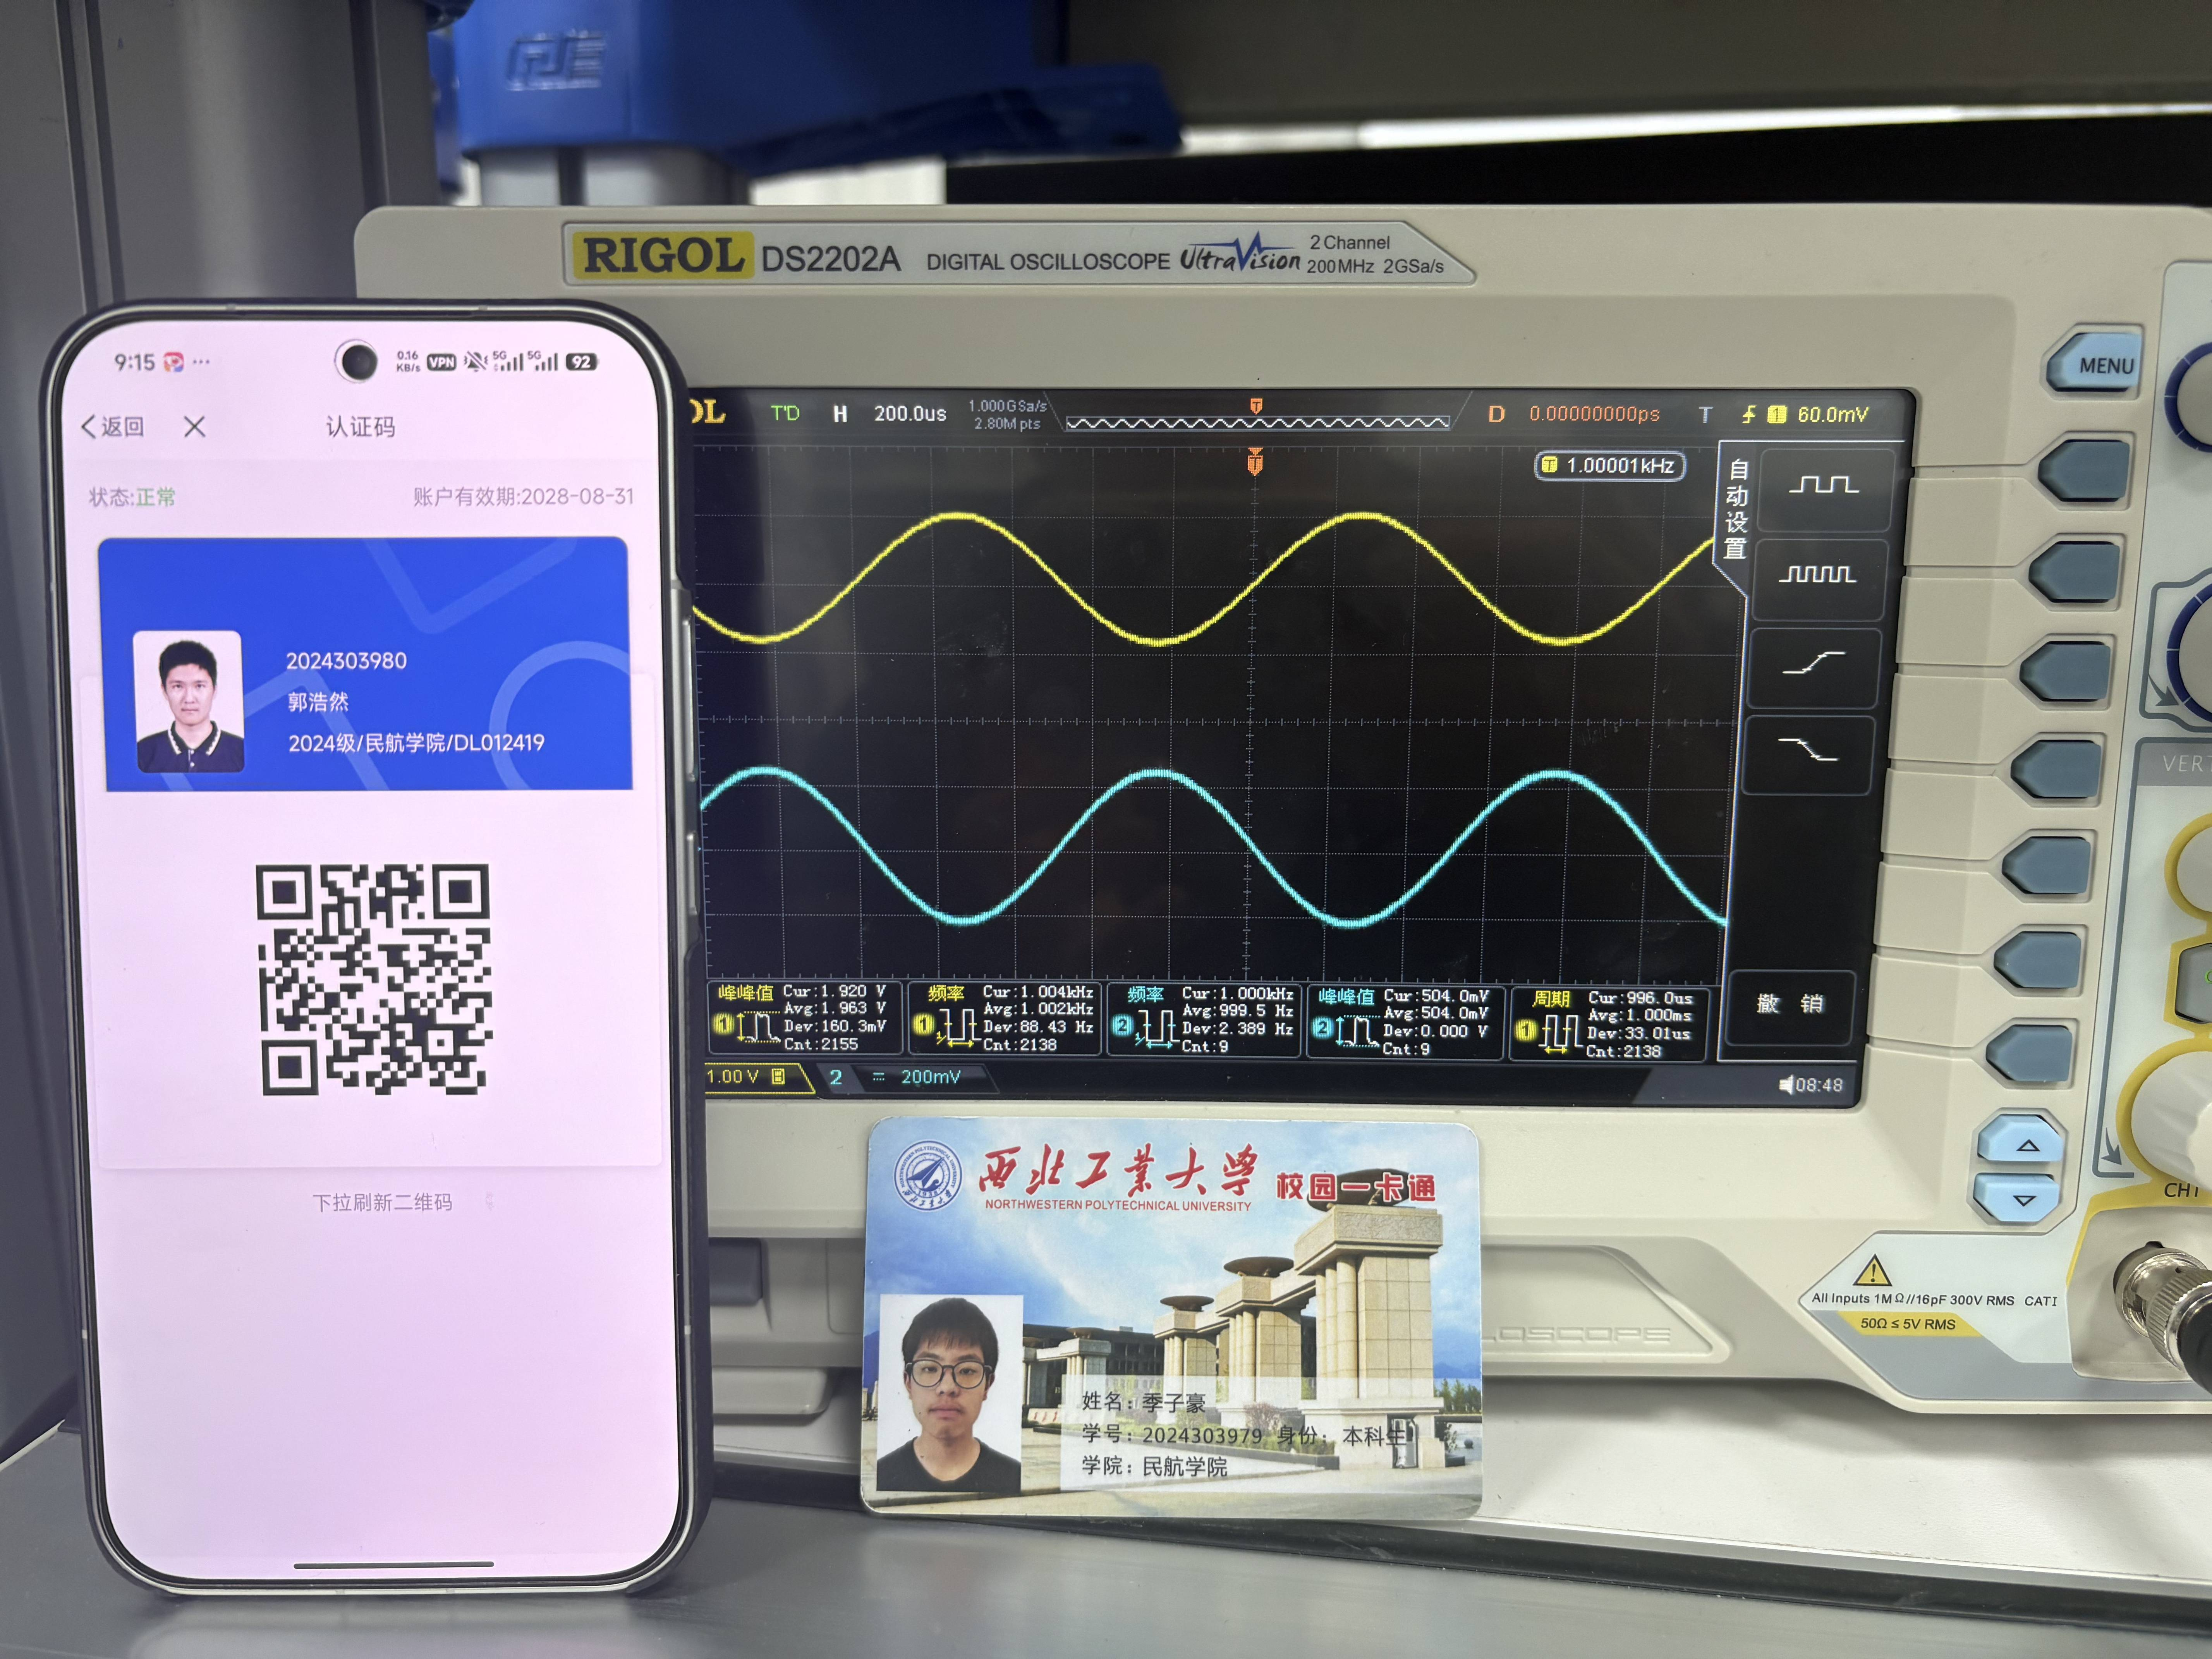
\includegraphics[width=\textwidth]{./5. sample/figures/恢复2k.jpg}
        \caption{$f_s = \SI{2}{kHz}$}
    \end{subfigure}
    
    \vspace{0.5cm} % 上下两行间距
    
    \begin{subfigure}[b]{0.45\textwidth}
        \centering
        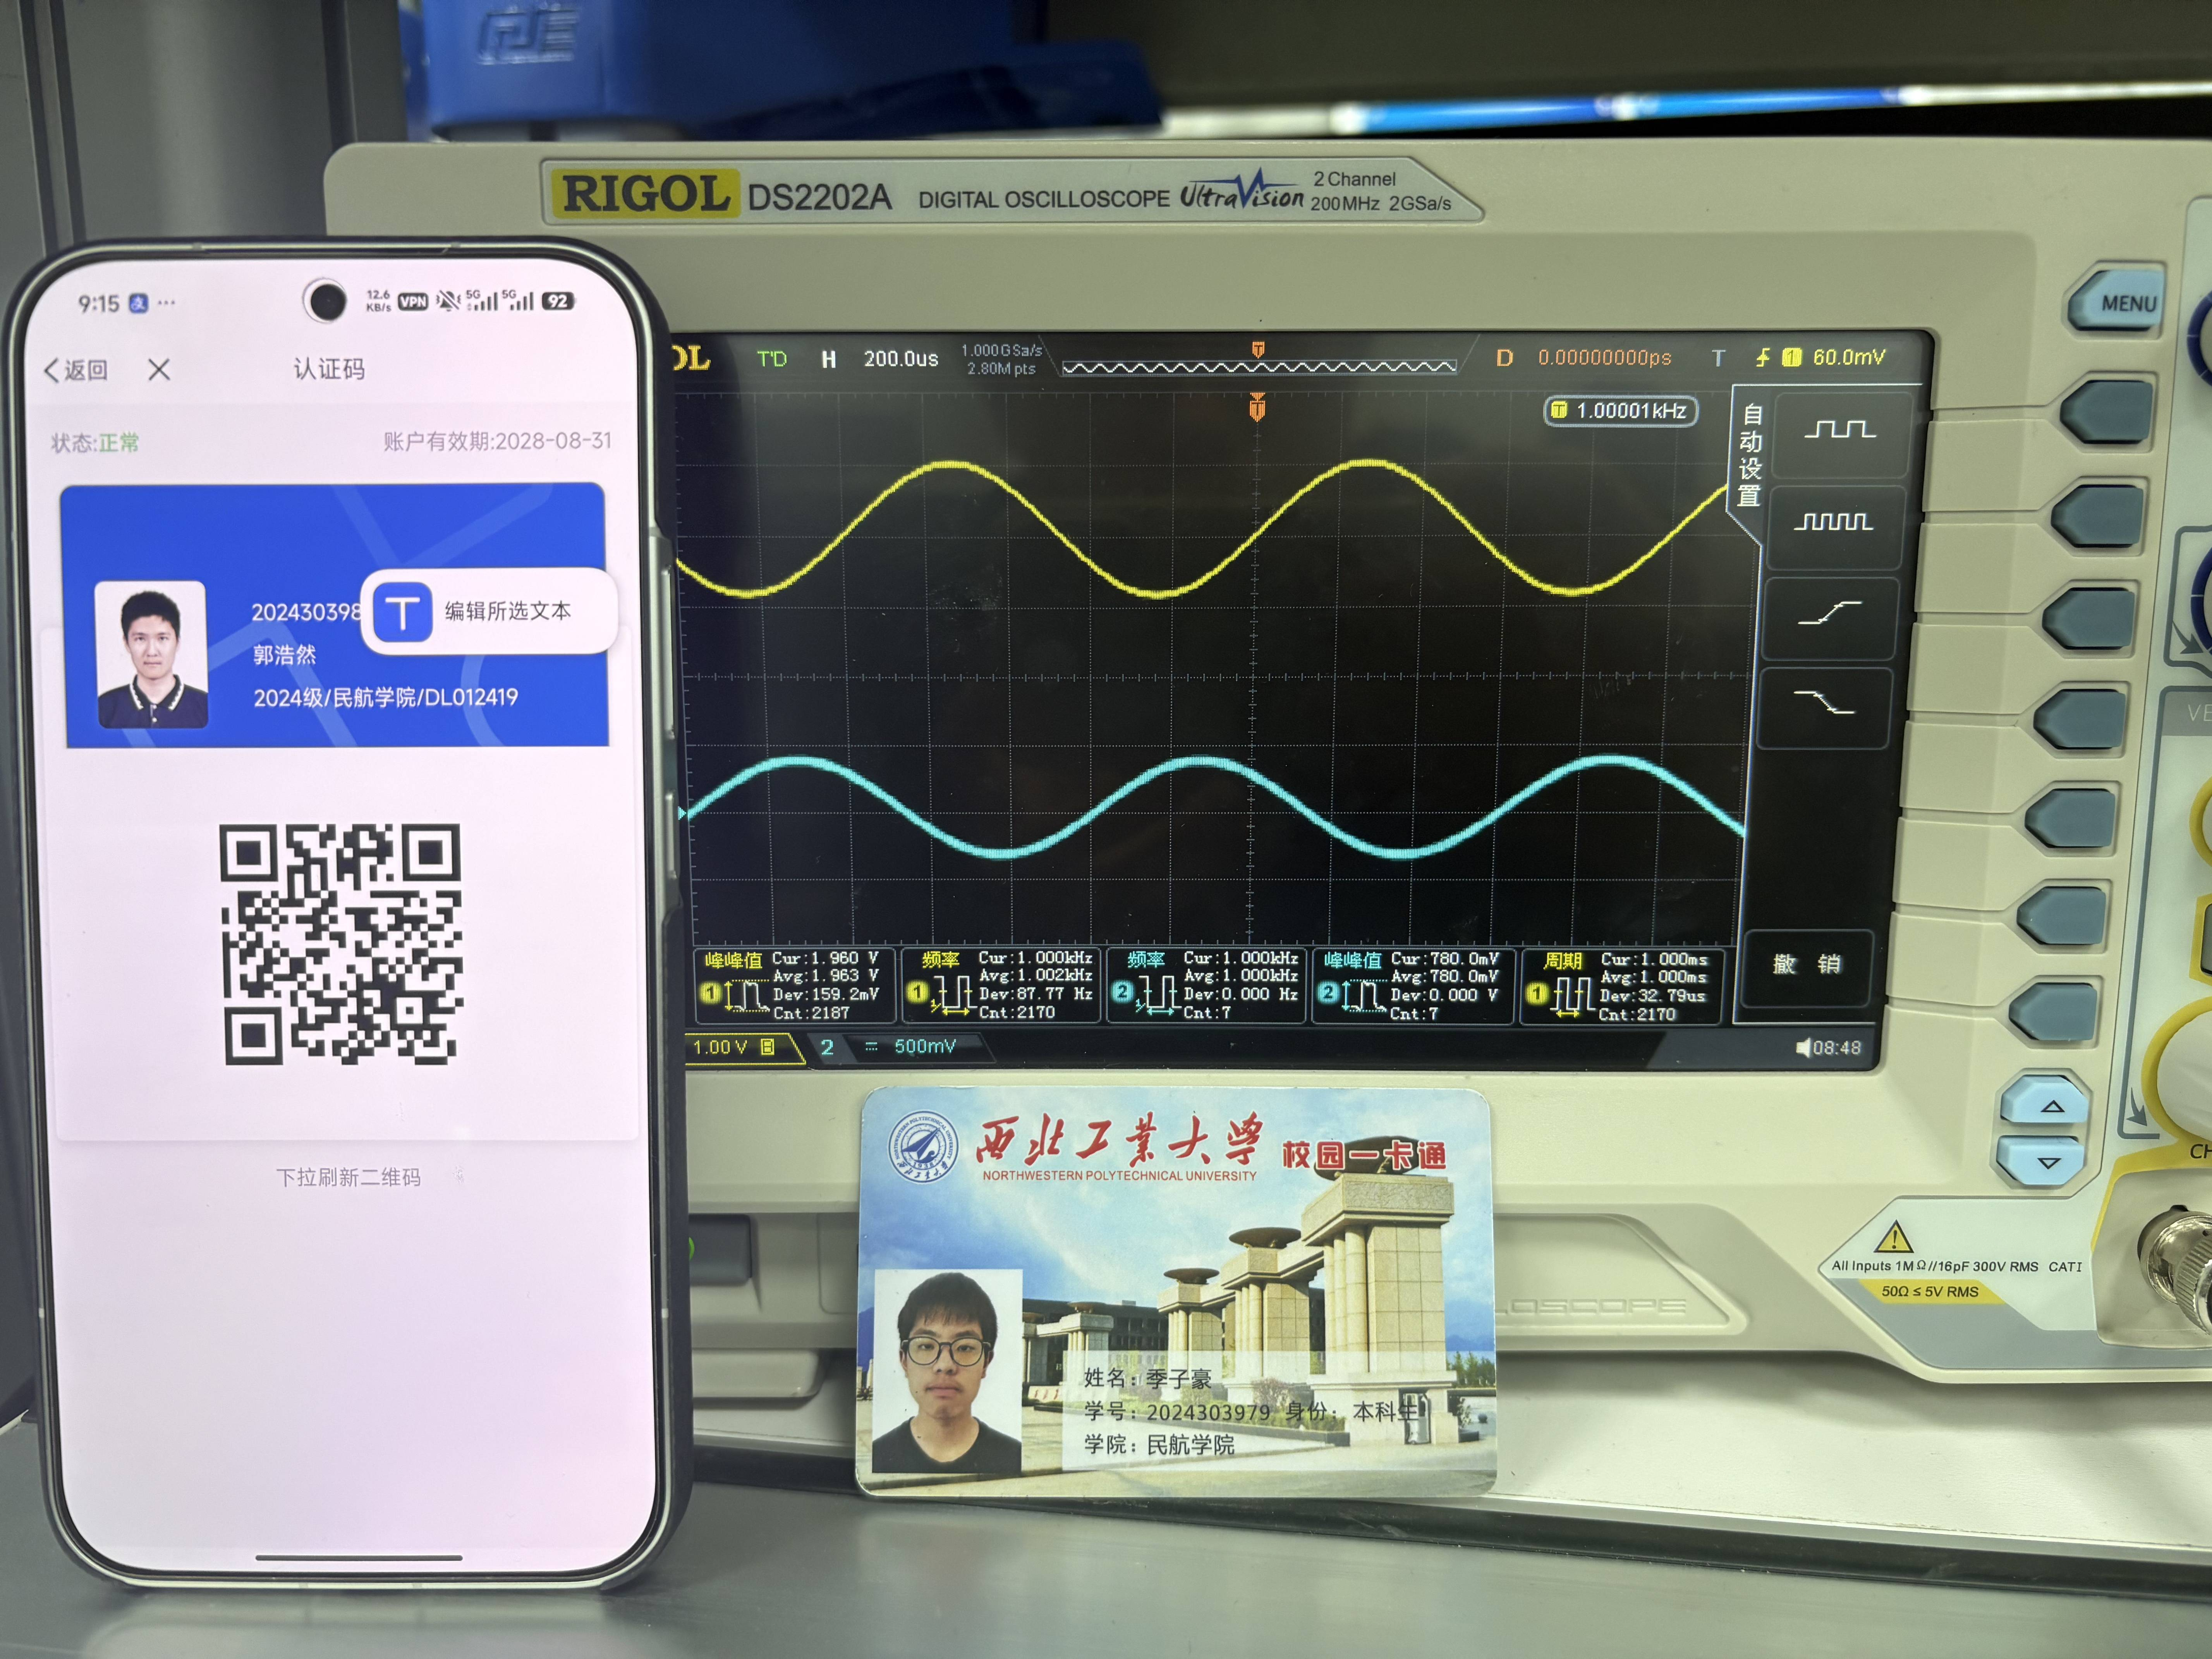
\includegraphics[width=\textwidth]{./5. sample/figures/恢复4k.jpg}
        \caption{$f_s = \SI{4}{kHz}$}
    \end{subfigure}
    \hfill
    \begin{subfigure}[b]{0.45\textwidth}
        \centering
        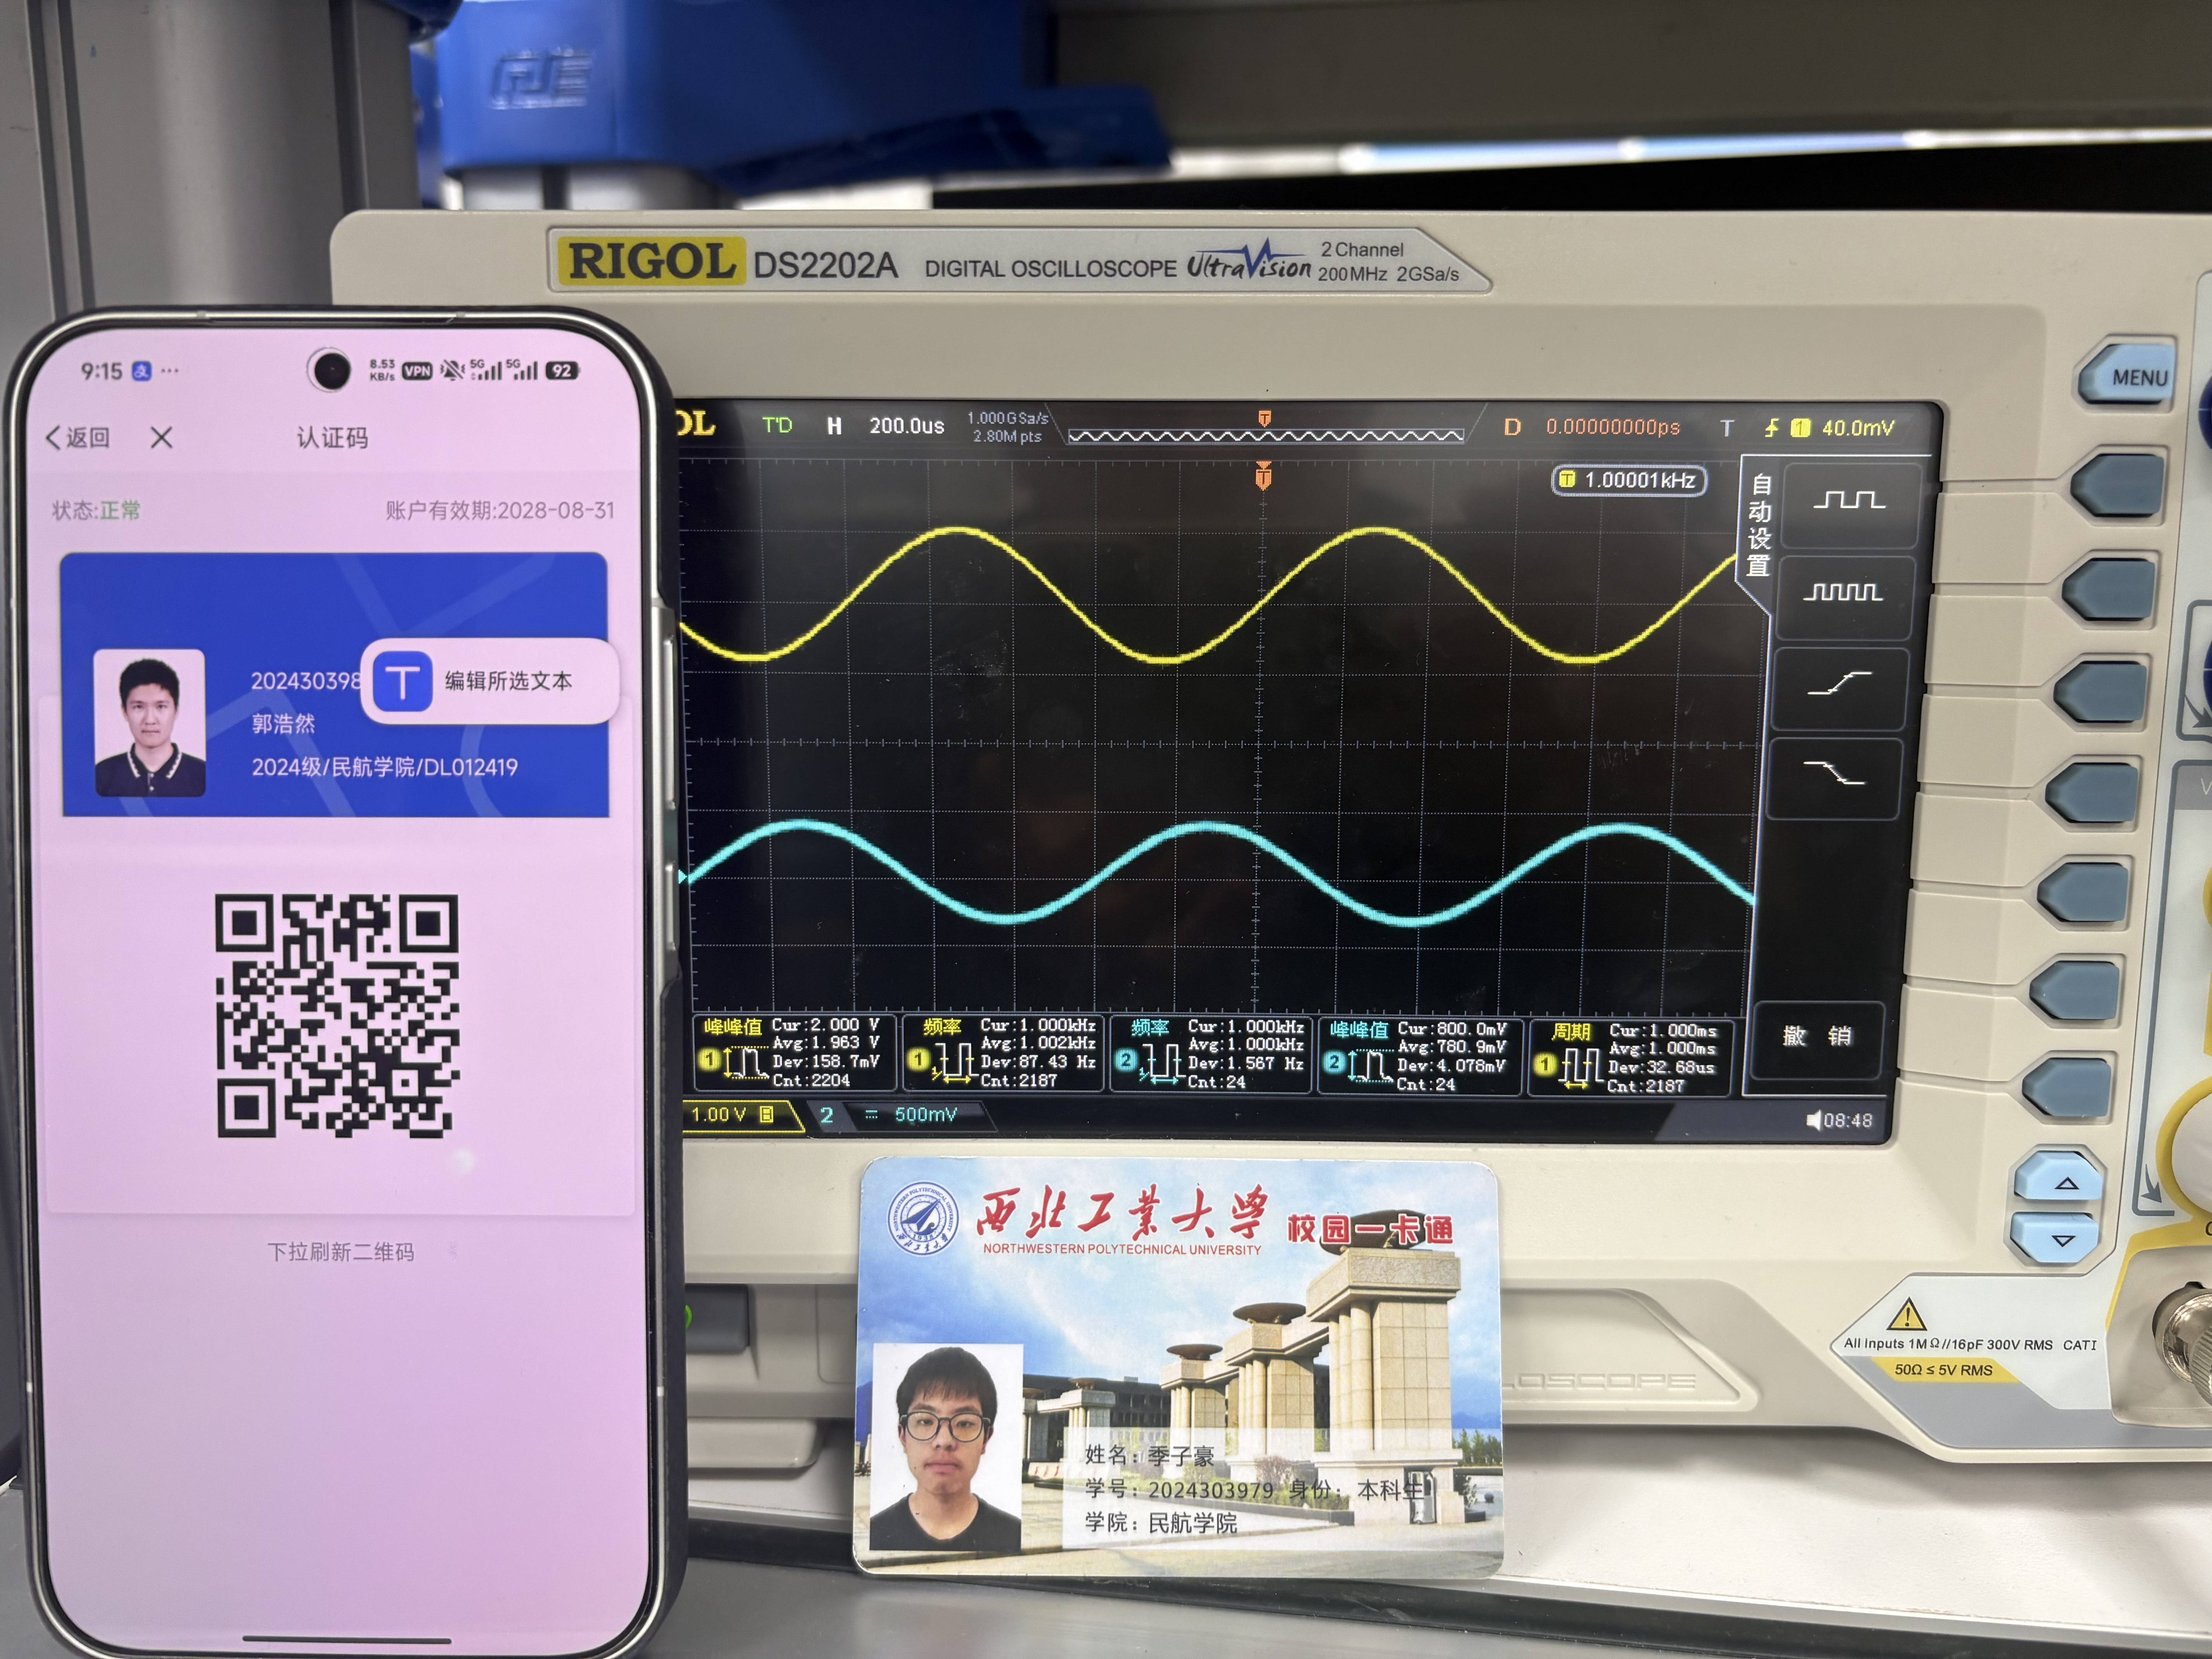
\includegraphics[width=\textwidth]{./5. sample/figures/恢复8k.jpg}
        \caption{$f_s = \SI{8}{kHz}$}
    \end{subfigure}
    \caption{恢复信号波形观测 (蓝色：恢复信号，黄色：输入信号)}
    \label{fig:recovery}
\end{figure}


% ================= 六、实验结论 =================
\section{实验结论}
\subsection{同步抽样与异步抽样的特点对比}
通过观察示波器波形，我们可以总结出同步抽样与异步抽样的主要区别：
\begin{itemize}
    \item \textbf{同步抽样}：抽样时钟与信号源由同一晶振产生，时间严格对齐。
    \begin{itemize}
        \item \textbf{优点}：波形稳定，无相位漂移，便于观察和分析。
        \item \textbf{适用场景}：适合周期性信号处理及理论验证实验。
    \end{itemize}
    \item \textbf{异步抽样}：抽样时钟与信号源独立，存在频率和相位的微小差异。
    \begin{itemize}
        \item \textbf{特点}：示波器上观察到的波形存在相位抖动（漂移），难以锁定。
        \item \textbf{意义}：更符合实际通信系统中收发端时钟不完全同步的真实情况。
    \end{itemize}
\end{itemize}
\subsection{系统参数对信号恢复的影响}
\begin{enumerate}
    \item \textbf{抽样率 ($f_s$) 的影响}：
    实验验证了奈奎斯特抽样定理。
    \begin{itemize}
        \item 当 $f_s < 2f_m$ (如 \SI{1}{kHz} 抽样 \SI{1.7}{kHz} 信号) 时，发生频谱混叠，恢复出的信号严重失真。
        \item 当 $f_s \gg 2f_m$ (如 \SI{8}{kHz} 抽样) 时，频谱延拓分量间隔大，低通滤波器能轻松滤出原信号，恢复波形光滑且幅度准确。
    \end{itemize}
    
    \item \textbf{滤波器 ($f_c$) 的影响}：
    低通滤波器是信号恢复的关键。其截止频率 $f_c$ 必须满足 $f_m < f_c < f_s - f_m$。
    \begin{itemize}
        \item 若滤波器阶数不够或截止特性不陡峭，可能会残留部分高频延拓分量，导致恢复信号中含有高频噪声（锯齿状波纹）。
        \item 本实验采用的 8 阶有源低通滤波器具有较好的带外衰减特性，有效保证了过采样时的信号恢复质量。
    \end{itemize}
\end{enumerate}
% ================= 七、MATLAB 课后作业 =================
\section{MATLAB 课后作业}

\subsection{任务一：$Sa(t)$ 信号的抽样与重构}
\textbf{题目要求}：结合抽样定理，利用 MATLAB 编程实现 $Sa(t)$ 信号经过冲激脉冲抽样后得到的抽样信号 $f_s(t)$ 及其频谱，并利用 $f_s(t)$ 构建 $Sa(t)$ 信号，计算重建信号与原信号的误差。

得到的波形及误差分析如图 \ref{fig:hw_sa} 所示。

\begin{figure}[H]
    \centering
    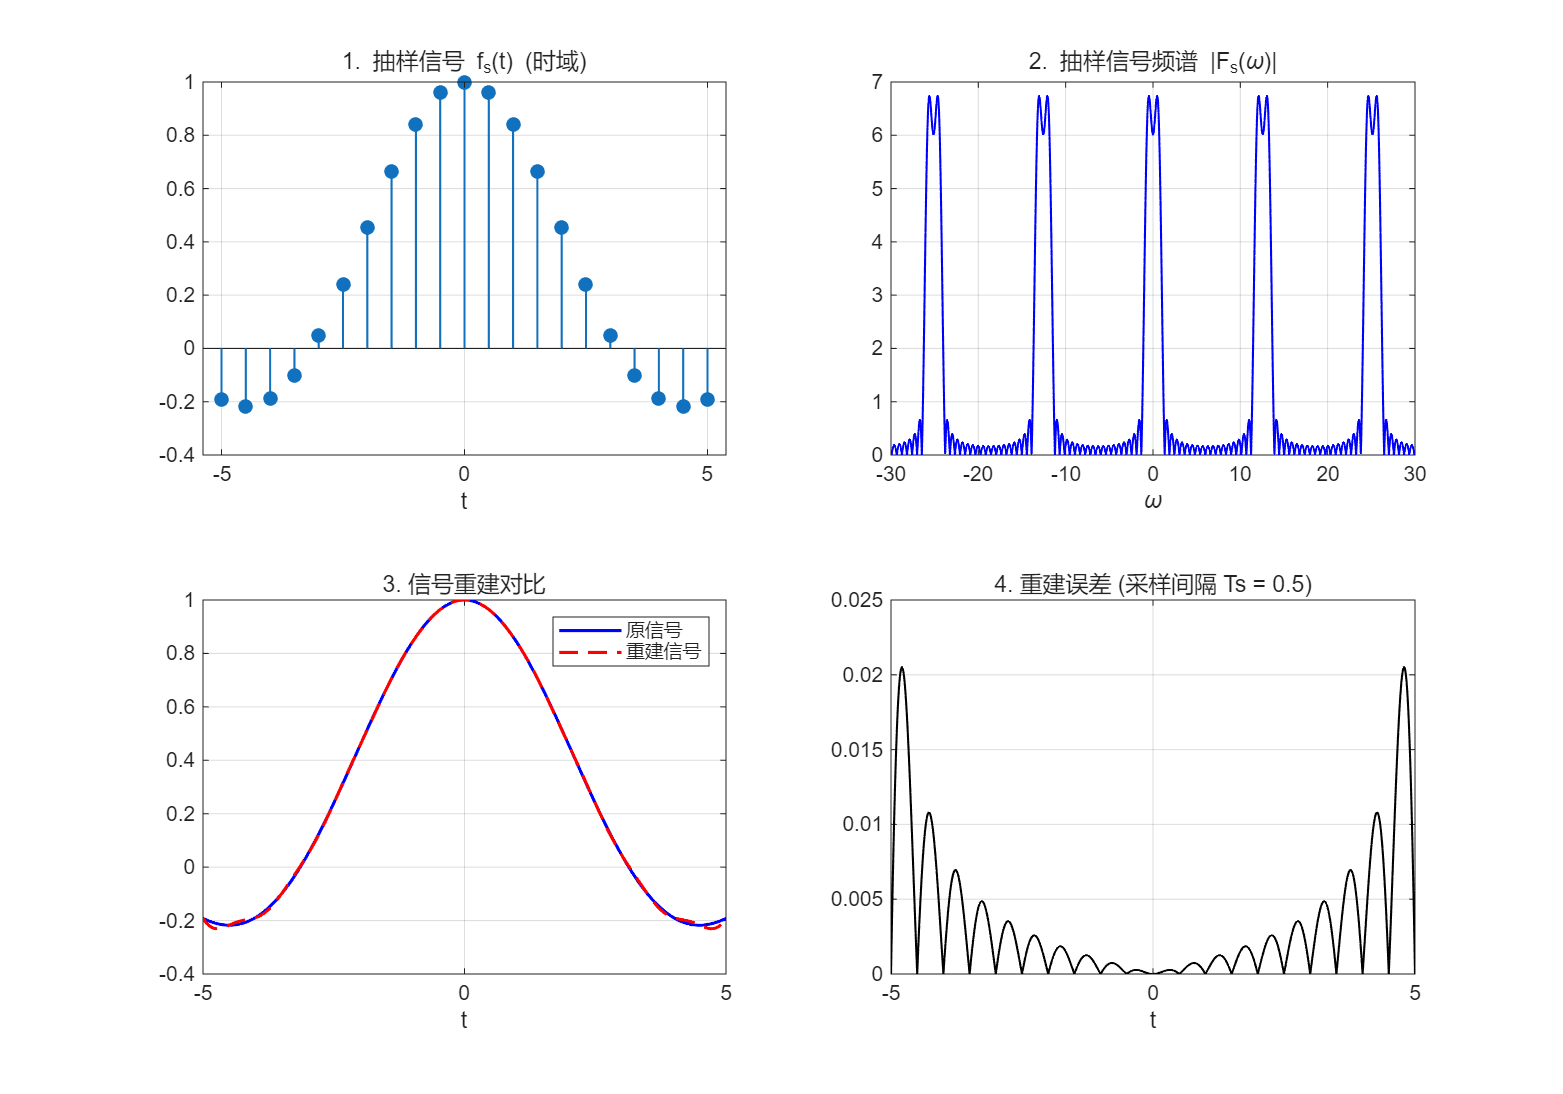
\includegraphics[width=\textwidth]{./5. sample/figures/sample2.png}
    \caption{$Sa(t)$ 信号的抽样、重构与误差分析}
    \label{fig:hw_sa}
\end{figure}

\subsection{任务二：升余弦信号的抽样与重构}
\textbf{题目要求}：结合抽样定理，利用 MATLAB 编程实现升余弦信号：
\begin{equation}
    f(t) = \frac{E}{2} \left( 1 + \cos\frac{\pi t}{\tau} \right), \quad |t| \le \tau
\end{equation}
其中 $E=1, \tau=\pi$。经过冲激脉冲抽样后得到抽样信号 $f_s(t)$ 及其频谱，利用 $f_s(t)$ 构建升余弦信号，并计算误差。


得到的波形及误差分析如图 \ref{fig:hw_cos} 所示。

\begin{figure}[H]
    \centering
    
    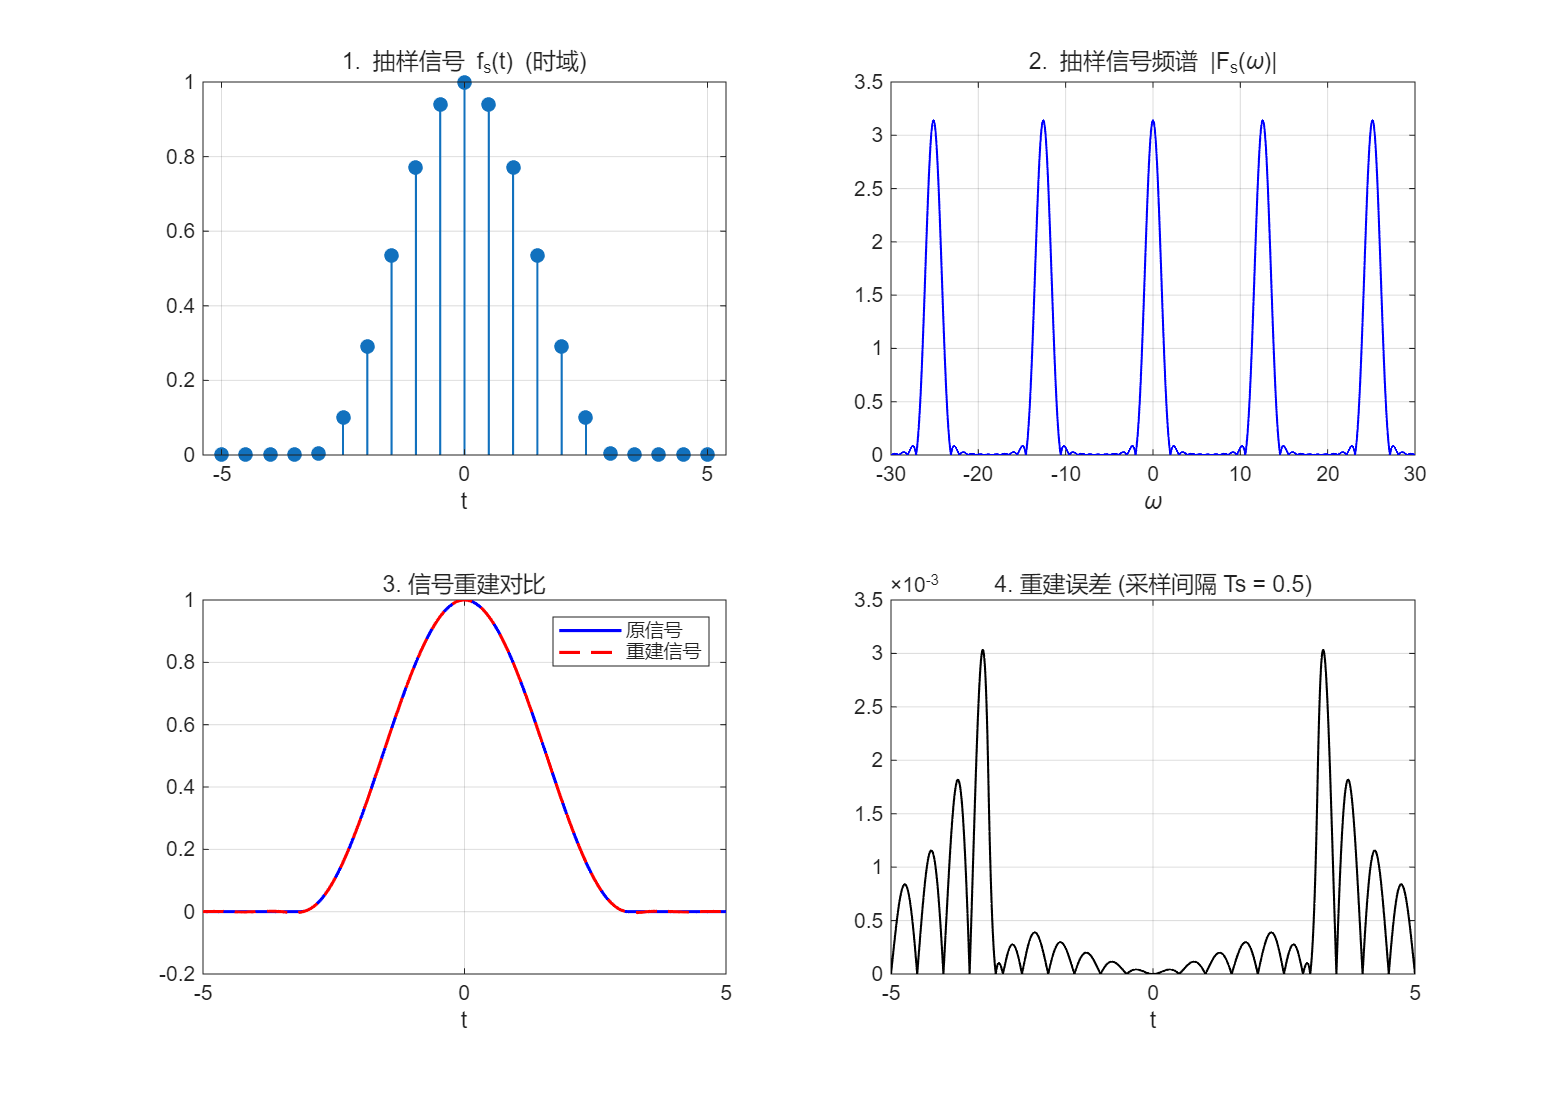
\includegraphics[width=\textwidth]{./5. sample/figures/sample.png}
    \caption{升余弦信号的抽样、重构与误差分析}
    \label{fig:hw_cos}
\end{figure}


% ===================================================================
% 第六章：信号的分解与合成 (Origin: 6. filter)
% ===================================================================
\chapter{信号的分解与合成}

% ----------------------------------------------------------------------
% 第一部分：实验目的
% ----------------------------------------------------------------------
\section{实验目的}
\begin{enumerate}
    \item 了解和熟悉波形分解与合成的原理。
    \item 了解和掌握用傅里叶级数进行谐波分析的方法。
\end{enumerate}
% ----------------------------------------------------------------------
% 第二部分：实验器材
% ----------------------------------------------------------------------
\section{实验器材}
\begin{table}[H]
    \centering
    \caption{实验器材列表}
    \begin{tabular}{clc}
        \toprule
        \textbf{序号} & \textbf{器材名称} & \textbf{数量} \\
        \midrule
        1 & 双踪示波器 & 1台 \\
        2 & 数字万用表 & 1台 \\
        3 & 信号源及频率计模块 (S2模块) & 1块 \\
        4 & 数字信号处理模块 (S4模块) & 1块 \\
        \bottomrule
    \end{tabular}
\end{table}
% ----------------------------------------------------------------------
% 第三部分：实验原理
% ----------------------------------------------------------------------
\section{实验原理}
\subsection{信号的频谱}
满足狄利克雷条件的周期信号 $f(t)$ 可展开为傅里叶级数。对于周期为 $T$ 的信号，其三角形式展开为：
\begin{equation}
    f(t) = a_0 + \sum_{n=1}^{\infty} (a_n \cos n\Omega t + b_n \sin n\Omega t)
\end{equation}
其中 $\Omega = \frac{2\pi}{T}$。通过将信号分解为直流分量及各次谐波分量，可以研究其频谱分布。
\subsection{方波信号的分解}
对于幅度为 $A$，占空比为 $50\%$ 的方波信号，其傅里叶级数展开式仅包含奇次谐波：
\begin{equation}
    f(t) = \frac{4A}{\pi} \left( \sin \omega t + \frac{1}{3} \sin 3\omega t + \frac{1}{5} \sin 5\omega t + \dots \right)
\end{equation}
各次谐波幅度理论值为 $V_n = \frac{4A}{n\pi}$ ($n=1,3,5\dots$)。
对于占空比为 $\tau/T$ 的矩形波，其各次谐波幅度由下式决定：
\begin{equation}
    |c_n| = \frac{2A}{n\pi} |\sin(n\pi \cdot \frac{\tau}{T})| \times 2 = \frac{4A}{n\pi} |\sin(n\pi \cdot \frac{\tau}{T})|
\end{equation}

\subsection{三角波信号的分解}
三角波信号的傅里叶级数展开式为：
\begin{equation}
    f(t) = \frac{8A}{\pi^2} \sum_{n=1,3,5\dots}^{\infty} \frac{1}{n^2} \cos(n\omega t)
\end{equation}
其谐波幅度随 $1/n^2$ 衰减，收敛速度快于方波。
% ----------------------------------------------------------------------
% 第四部分：实验步骤
% ----------------------------------------------------------------------
\section{实验步骤}
\subsection{任务一：方波的分解}
\begin{enumerate}
    \item 连接 S2 模块 P2 端口与 S4 模块 P9 端口。
    \item 设置 S2 输出幅度 2V，频率分别为 400Hz 和 600Hz 的方波（占空比分别调整为 50\% 和 40\%）。
    \item 将 S4 模块 SW1 拨至 ``00000101''，S3 拨至 ``00000000''。
    \item 使用示波器在 TP1 $\sim$ TP7 观测各次谐波，在 TP8 观测高次谐波。
\end{enumerate}
\subsection{任务二：方波的合成}
\begin{enumerate}
    \item 调节 S3 拨码开关，按照基波、基波+3次、基波+3+5次等组合控制谐波叠加。
    \item 在 TP8 处观察合成波形，并与原始信号对比。
\end{enumerate}
\subsection{任务三：三角波的分解与合成}
\begin{enumerate}
    \item 设置 S2 输出幅度 2V 的三角波（400Hz/600Hz）。
    \item 重复上述分解与合成步骤，记录数据并观察波形。
\end{enumerate}
% ----------------------------------------------------------------------
% 第五部分：实验数据与分析
% ----------------------------------------------------------------------
\section{实验数据与分析}
\subsection{方波信号分解数据}
% 表1：占空比 50%
\begin{table}[H]
    \centering
    \caption{占空比 50\% 方波信号频谱数据 ($A=2\text{V}$)}
    \label{tab:sq50}
    \begin{tabular}{lcccccccc}
        \toprule
        \textbf{谐波次数} & \textbf{1f} & \textbf{2f} & \textbf{3f} & \textbf{4f} & \textbf{5f} & \textbf{6f} & \textbf{7f} & \textbf{8f+} \\
        \midrule
        理论值 (V) & 2.55 & 0 & 0.85 & 0 & 0.51 & 0 & 0.36 & 0.65 \\
        400Hz 测量值 (V) & 2.60 & 0 & 1.12 & 0 & 0.76 & 0 & 0.64 & 0.32 \\
        600Hz 测量值 (V) & 2.60 & 0 & 1.08 & 0 & 0.76 & 0 & 0.64 & 0.32 \\
        \bottomrule
    \end{tabular}
\end{table}
% 表2：占空比 40%
\begin{table}[H]
    \centering
    \caption{占空比 40\% 方波信号频谱数据 ($A=2\text{V}$)}
    \label{tab:sq40}
    \begin{tabular}{lcccccccc}
        \toprule
        \textbf{谐波次数} & \textbf{1f} & \textbf{2f} & \textbf{3f} & \textbf{4f} & \textbf{5f} & \textbf{6f} & \textbf{7f} & \textbf{8f+} \\
        \midrule
        理论值 (V) & 2.42 & 0.75 & 0.50 & 0.61 & 0 & 0.40 & 0.21 & 0.63 \\
        400Hz 测量值 (V) & 2.56 & 1.04 & 0.80 & 0.88 & 0 & 0.72 & 0.52 & 0.32 \\
        600Hz 测量值 (V) & 2.56 & 1.04 & 0.76 & 0.92 & 0 & 0.72 & 0.56 & 0.36 \\
        \bottomrule
    \end{tabular}
\end{table}
\subsection{三角波信号分解数据}
% 表3：三角波
\begin{table}[H]
    \centering
    \caption{三角波信号频谱数据 ($A=2\text{V}$)}
    \label{tab:tri}
    \begin{tabular}{lcccccccc}
        \toprule
        \textbf{谐波次数} & \textbf{1f} & \textbf{2f} & \textbf{3f} & \textbf{4f} & \textbf{5f} & \textbf{6f} & \textbf{7f} & \textbf{8f+} \\
        \midrule
        理论值 (V) & 1.62 & 0 & 0.18 & 0 & 0.06 & 0 & 0.03 & 0.03 \\
        400Hz 测量值 (V) & 1.68 & 0 & 0.36 & 0 & 0.28 & 0 & 0.24 & 0 \\
        600Hz 测量值 (V) & 1.66 & 0 & 0.36 & 0 & 0.24 & 0 & 0.22 & 0 \\
        \bottomrule
    \end{tabular}
\end{table}


\subsection{信号分解频谱图}

% --- 第一组：400Hz 方波对比 (2张图) ---
\begin{figure}[H]
    \centering
    % 第一张：400Hz 40%
    \begin{subfigure}[b]{0.95\textwidth}
        \centering
        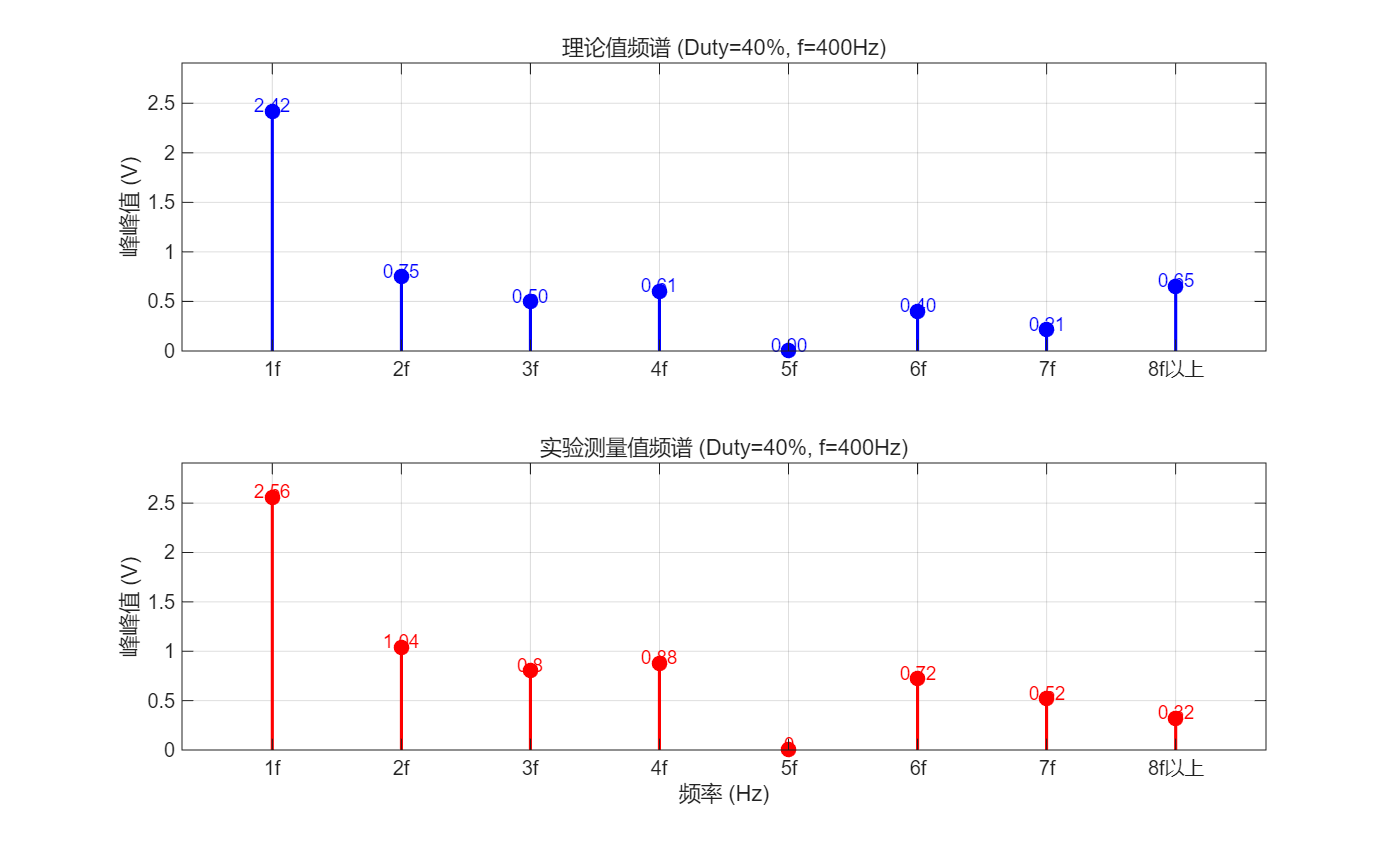
\includegraphics[width=\textwidth]{./6. filter/figures/f400_40.png} 
        \caption{方波 40\% (400Hz)}
    \end{subfigure}
    
    \vspace{0.5cm} % 图片间距
    
    % 第二张：400Hz 50%
    \begin{subfigure}[b]{0.95\textwidth}
        \centering
        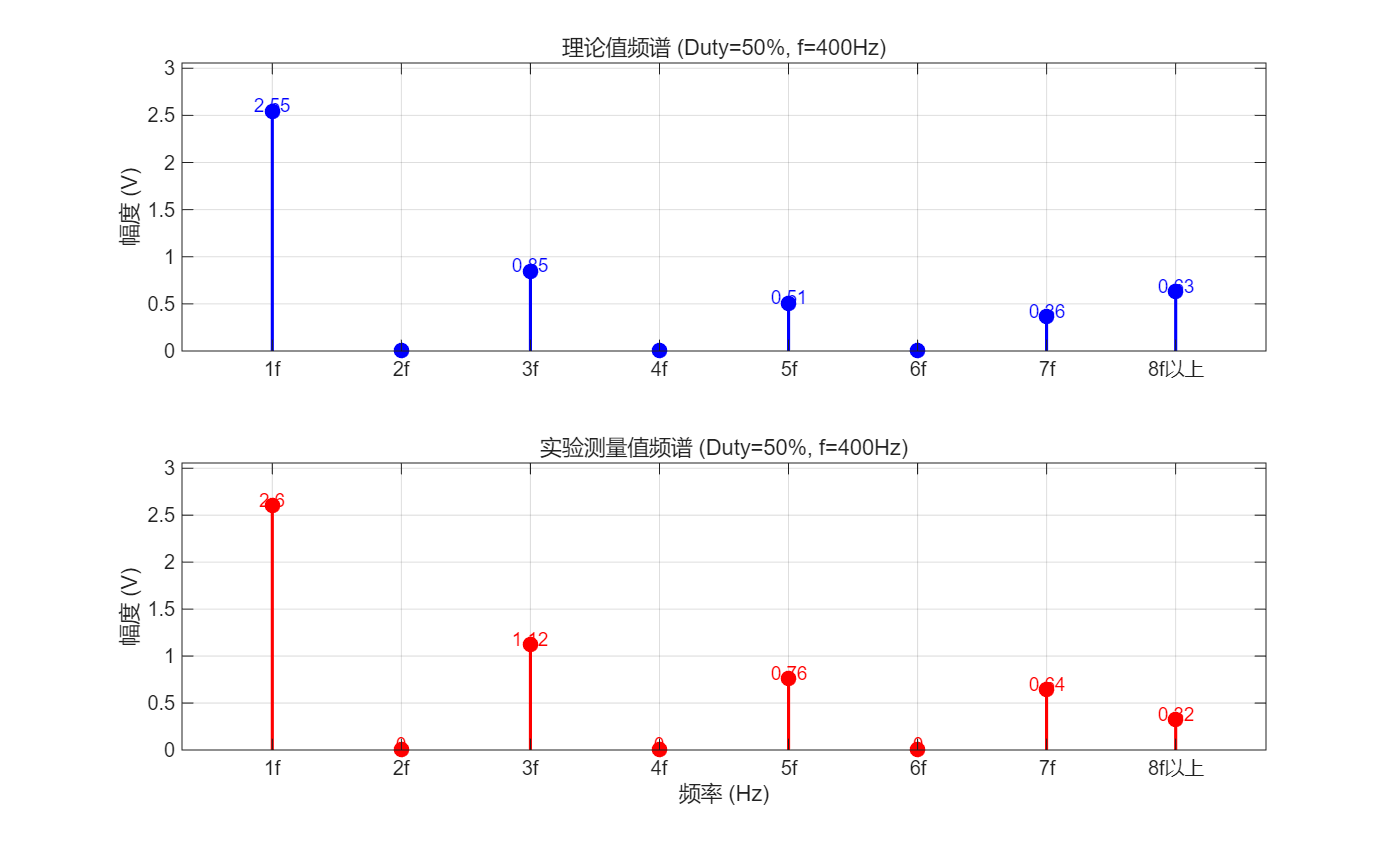
\includegraphics[width=\textwidth]{./6. filter/figures/f400_50.png}
        \caption{方波 50\% (400Hz)}
    \end{subfigure}
    \caption{400Hz 方波信号频谱测量图}
\end{figure}

% --- 第二组：600Hz 方波对比 (2张图) ---
\begin{figure}[H]
    \centering
    % 第一张：600Hz 40%
    \begin{subfigure}[b]{0.95\textwidth}
        \centering
        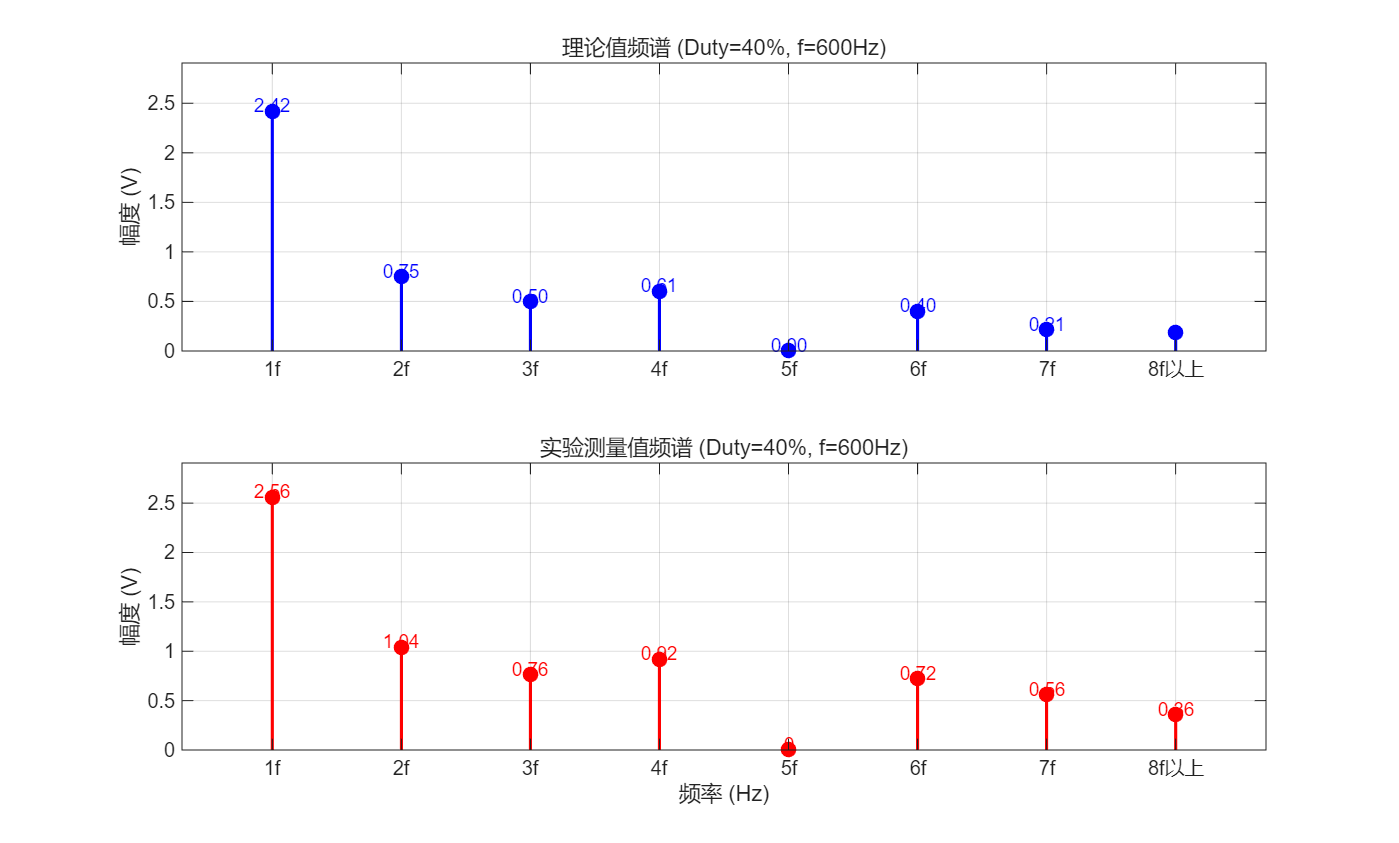
\includegraphics[width=\textwidth]{./6. filter/figures/f600_40.png}
        \caption{方波 40\% (600Hz)}
    \end{subfigure}
    
    \vspace{0.5cm}
    
    % 第二张：600Hz 50%
    \begin{subfigure}[b]{0.95\textwidth}
        \centering
        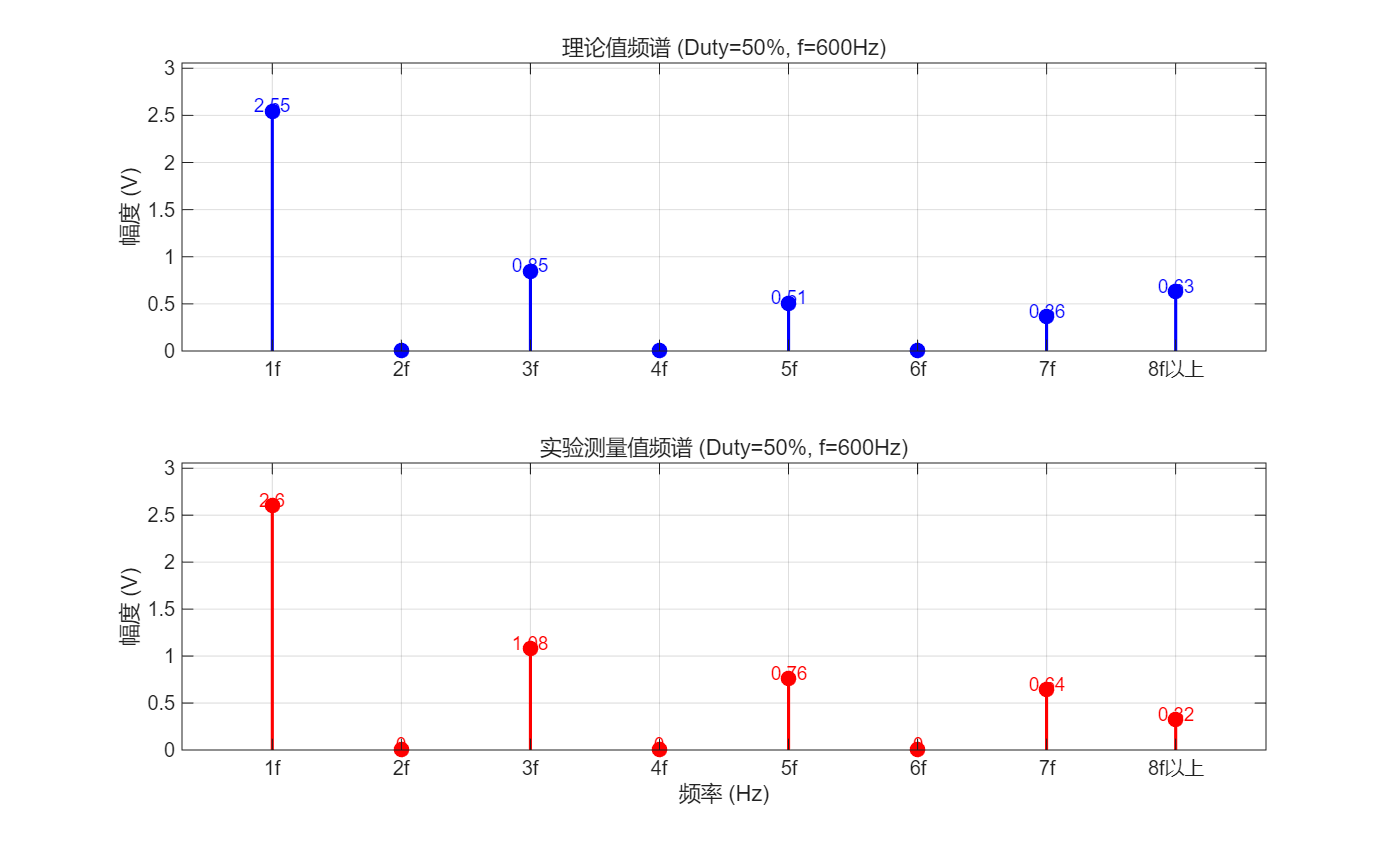
\includegraphics[width=\textwidth]{./6. filter/figures/f600_50.png}
        \caption{方波 50\% (600Hz)}
    \end{subfigure}
    \caption{600Hz 方波信号频谱测量图}
\end{figure}

% --- 第三组：三角波对比 (2张图) ---
\begin{figure}[H]
    \centering
    % 第一张：400Hz 三角波
    \begin{subfigure}[b]{0.95\textwidth}
        \centering
        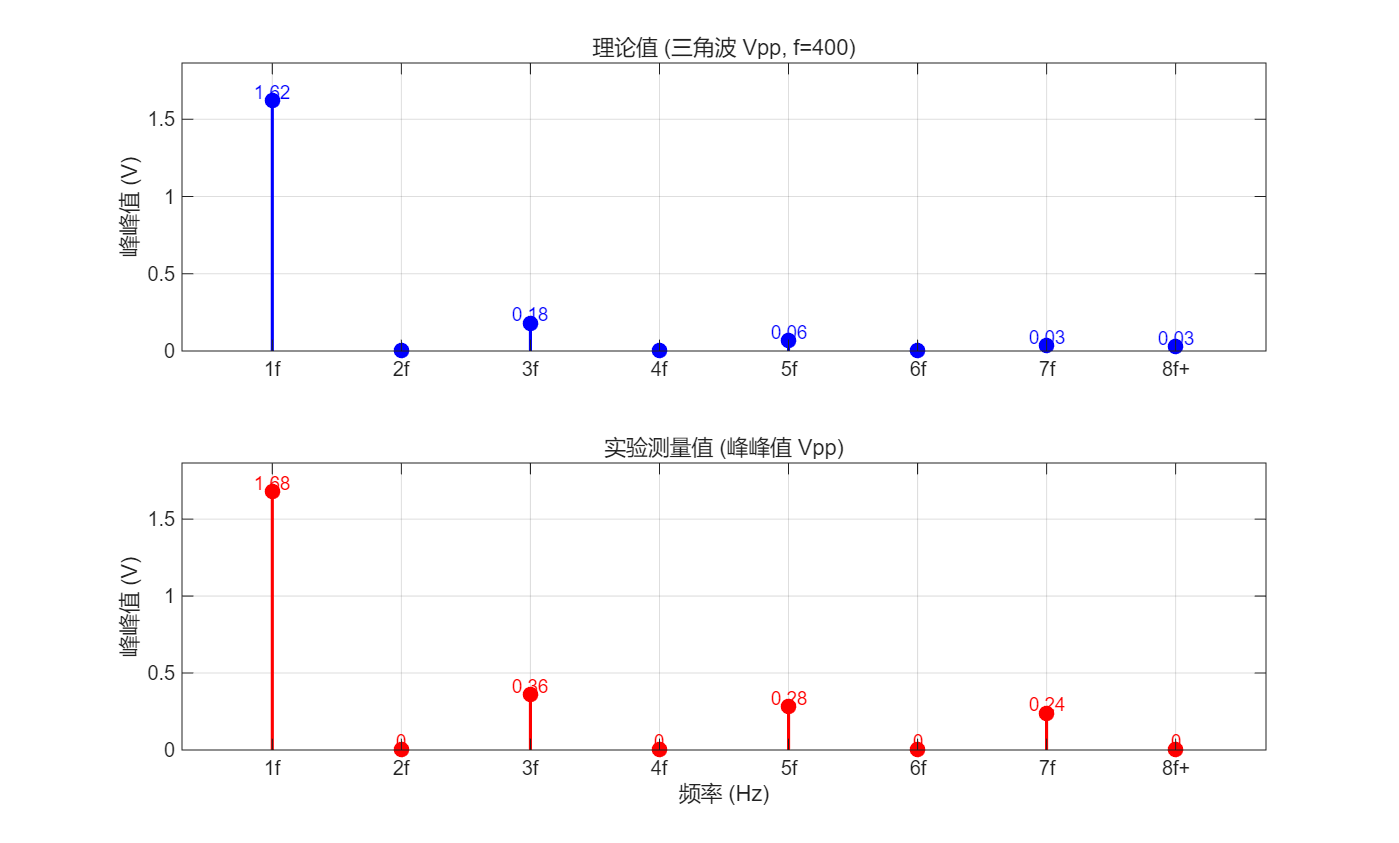
\includegraphics[width=\textwidth]{./6. filter/figures/f400.png}
        \caption{三角波 (400Hz)}
    \end{subfigure}
    
    \vspace{0.5cm}
    
    % 第二张：600Hz 三角波
    \begin{subfigure}[b]{0.95\textwidth}
        \centering
        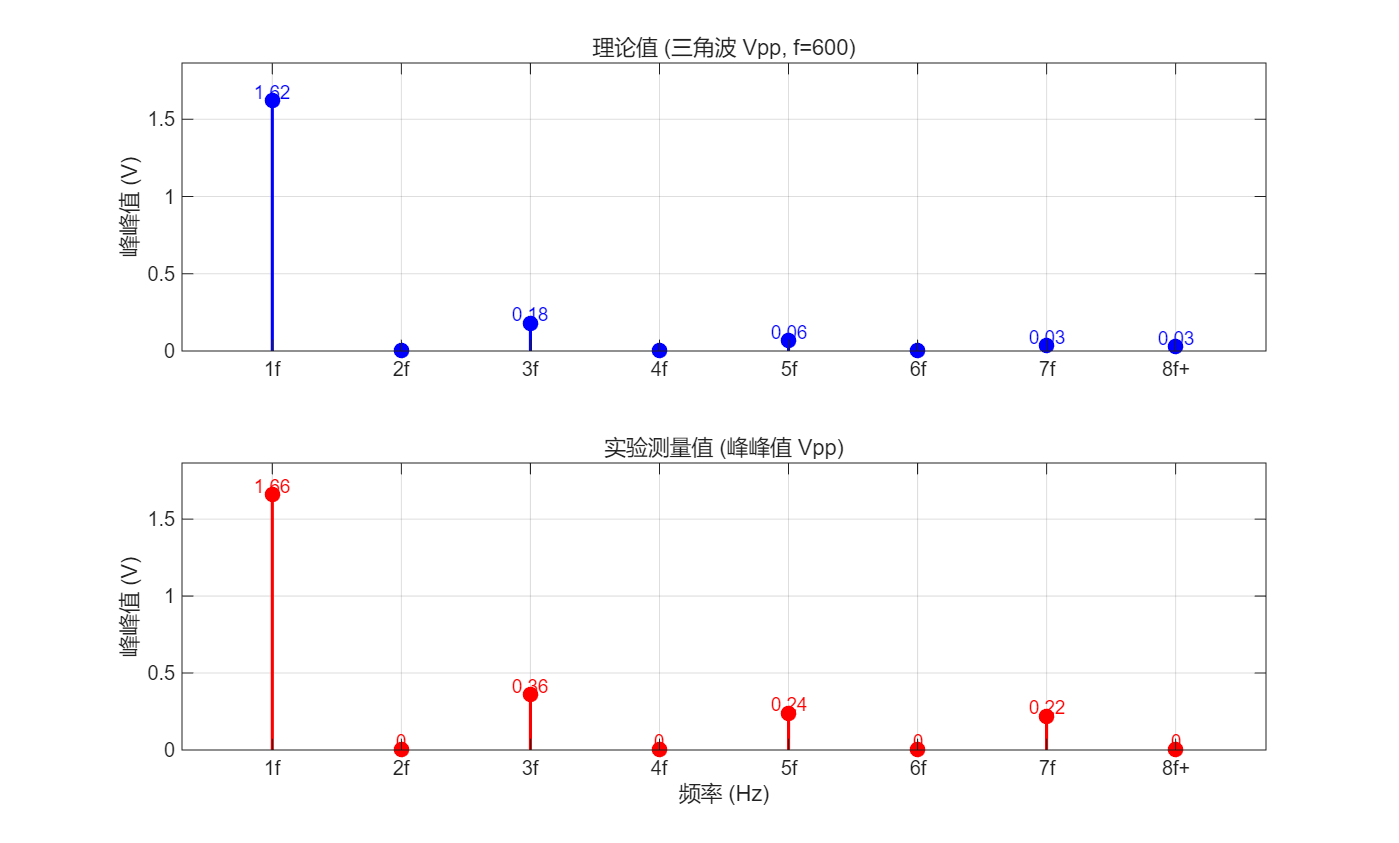
\includegraphics[width=\textwidth]{./6. filter/figures/f600.png}
        \caption{三角波 (600Hz)}
    \end{subfigure}
    \caption{三角波信号频谱测量图 (400Hz 与 600Hz)}
\end{figure}


\subsubsection{方波合成 (50\% 占空比, 400Hz)}

% --- 方波合成 Part 1 (前4张) ---
\begin{figure}[H]
    \centering
    % 第一行
    \begin{subfigure}[b]{0.48\textwidth}
        \centering
        
\includegraphics[width=\textwidth]{./6. filter/figures/square/1.jpg} 
        \caption{基波}
    \end{subfigure}
    \hfill
    \begin{subfigure}[b]{0.48\textwidth}
        \centering
        
\includegraphics[width=\textwidth]{./6. filter/figures/square/2.jpg} 
        \caption{基波+3次谐波}
    \end{subfigure}
    
    \vspace{0.3cm}
    
    % 第二行
    \begin{subfigure}[b]{0.48\textwidth}
        \centering
        
\includegraphics[width=\textwidth]{./6. filter/figures/square/3.jpg} 
        \caption{基波+5次谐波}
    \end{subfigure}
    \hfill
    \begin{subfigure}[b]{0.48\textwidth}
        \centering
        
\includegraphics[width=\textwidth]{./6. filter/figures/square/4.jpg} 
        \caption{1+3+5次谐波}
    \end{subfigure}
    \caption{方波信号合成过程 (1-4步)}
\end{figure}

% --- 方波合成 Part 2 (后4张) ---
\begin{figure}[H]
    \centering
    % 第一行 (即总第3行)
    \begin{subfigure}[b]{0.48\textwidth}
        \centering
        
\includegraphics[width=\textwidth]{./6. filter/figures/square/5.jpg} 
        \caption{全合成 (所有谐波)}
    \end{subfigure}
    \hfill
    \begin{subfigure}[b]{0.48\textwidth}
        \centering
        
\includegraphics[width=\textwidth]{./6. filter/figures/square/6.jpg} 
        \caption{缺3次谐波}
    \end{subfigure}
    
    \vspace{0.3cm}
    
    % 第二行 (即总第4行)
    \begin{subfigure}[b]{0.48\textwidth}
        \centering
        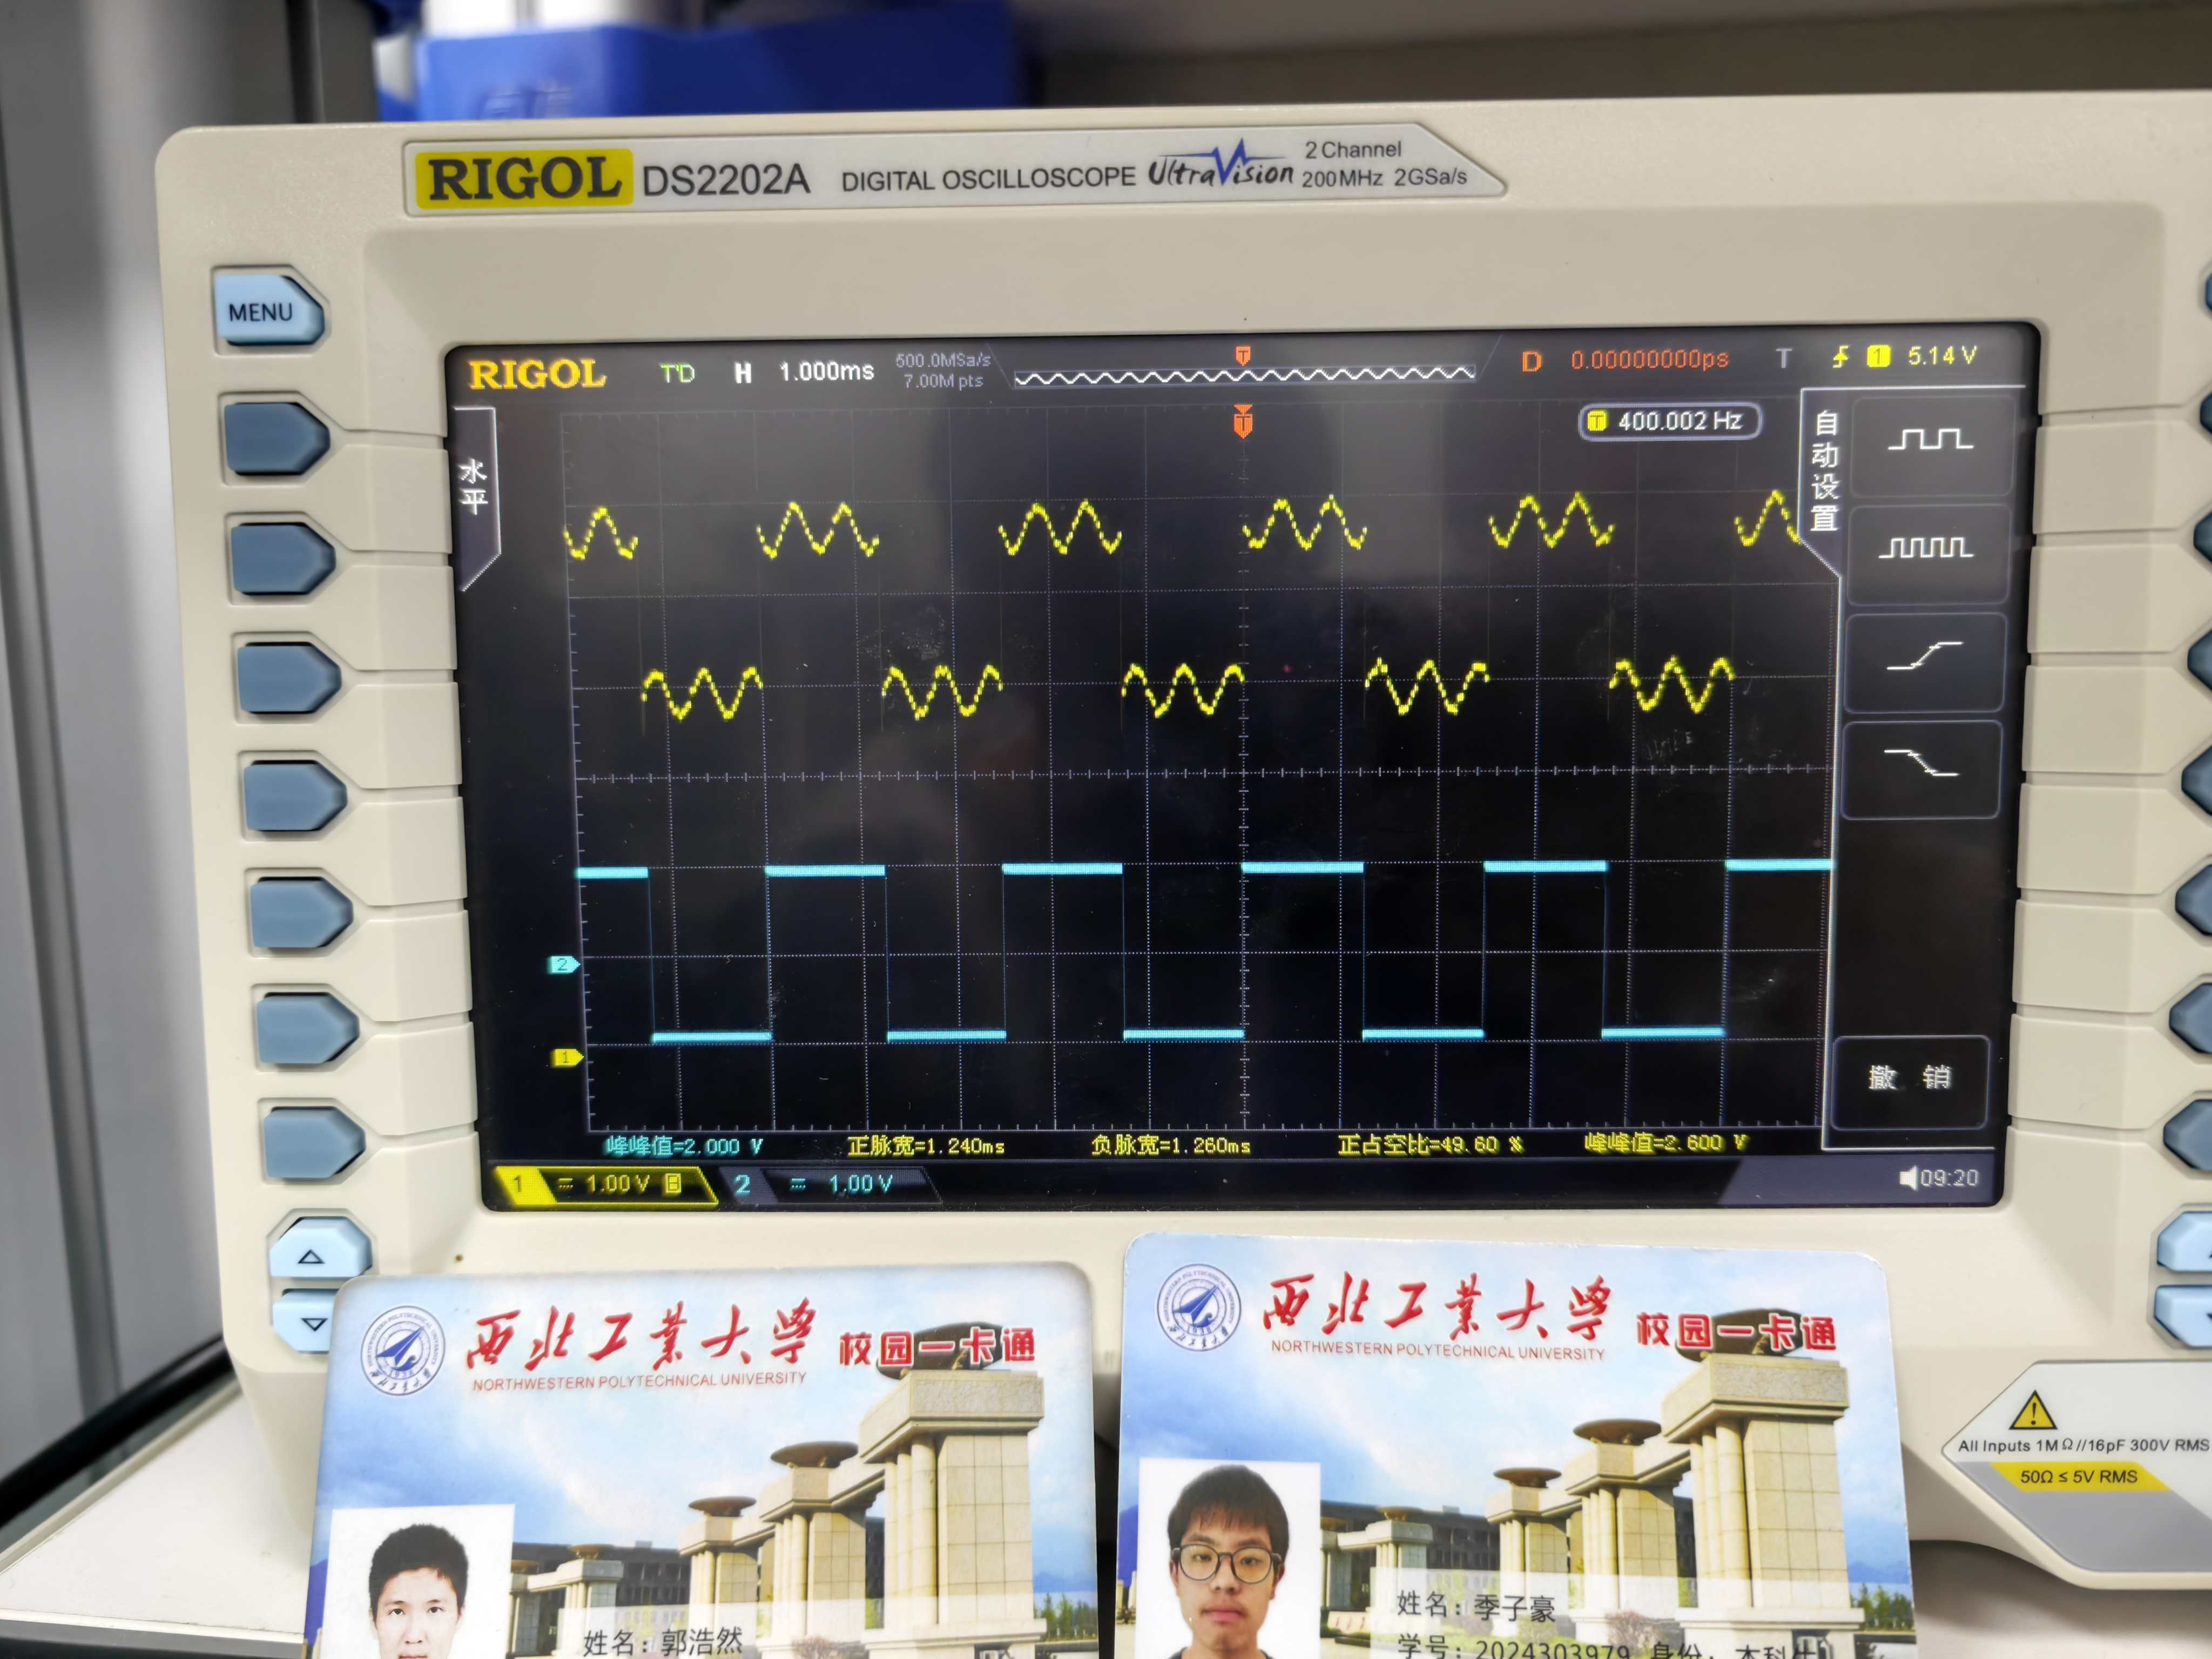
\includegraphics[width=\textwidth]{./6. filter/figures/square/7.jpg} 
        \caption{缺5次谐波}
    \end{subfigure}
    \hfill
    \begin{subfigure}[b]{0.48\textwidth}
        \centering
        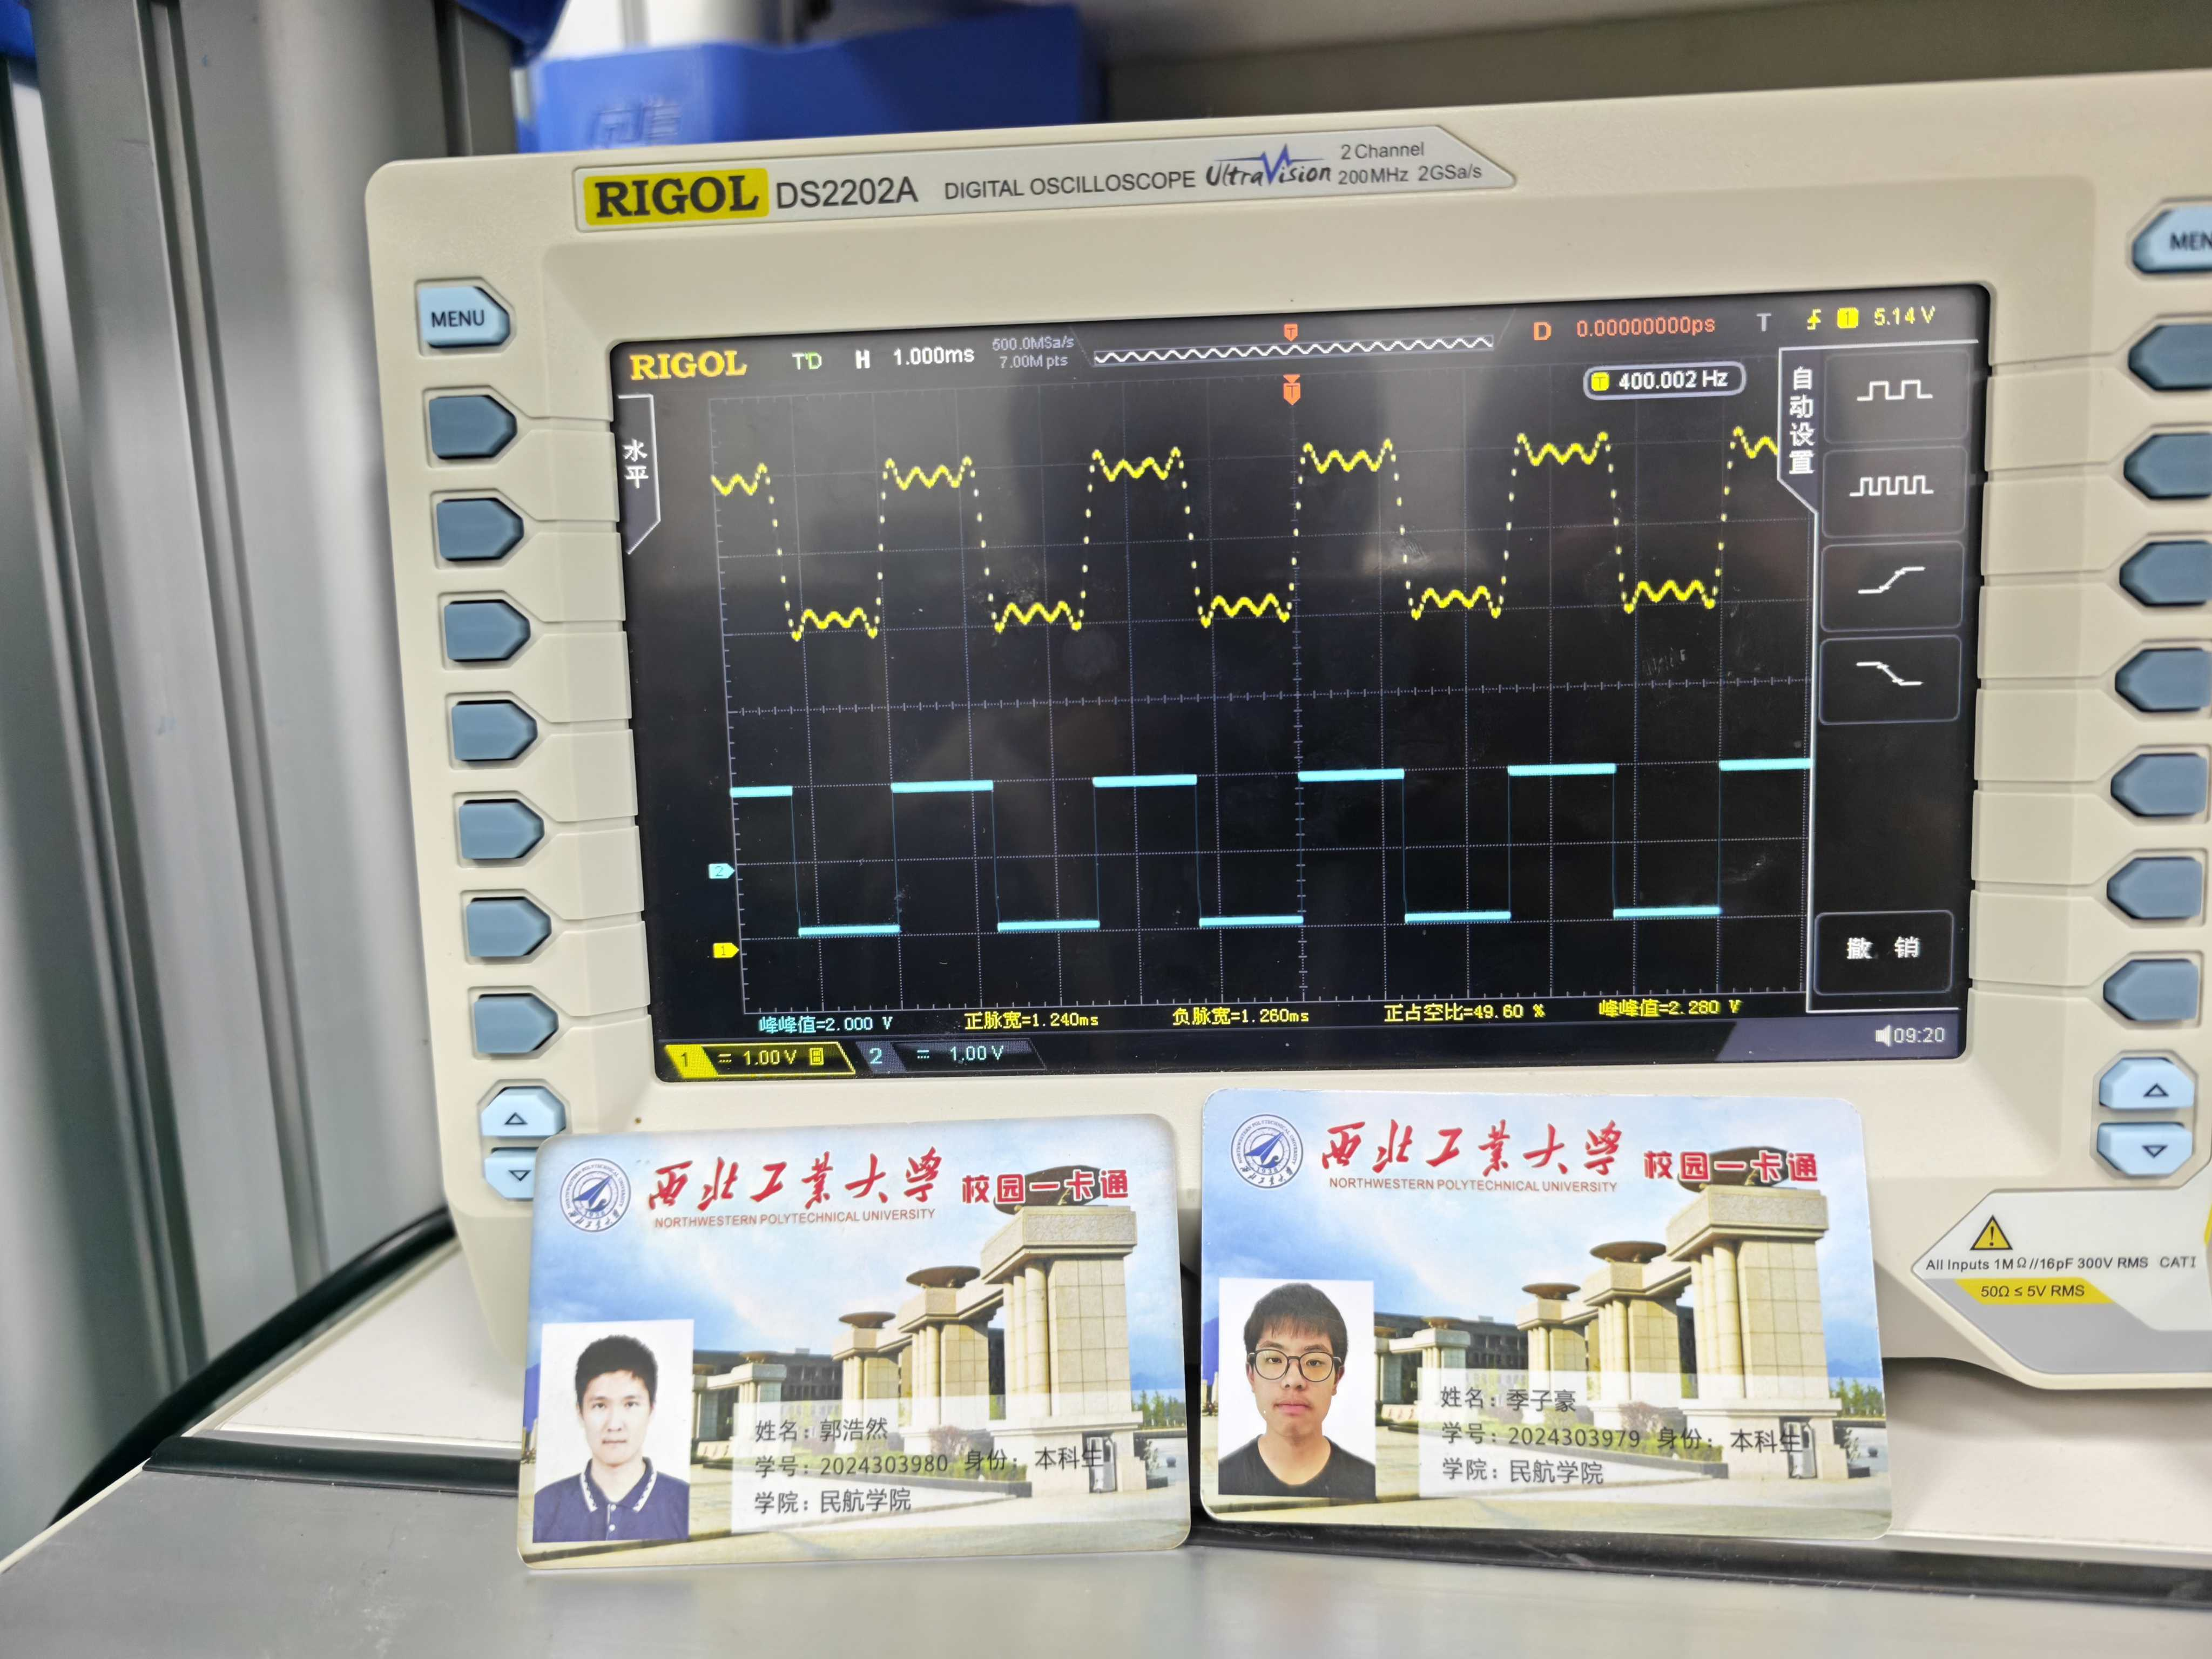
\includegraphics[width=\textwidth]{./6. filter/figures/square/8.jpg} 
        \caption{缺8次以上高次谐波}
    \end{subfigure}
    \caption{方波信号合成过程 (5-8步)}
\end{figure}

\subsubsection{三角波合成 (400Hz)}

% --- 三角波合成 Part 1 (前4张) ---
\begin{figure}[H]
    \centering
    \begin{subfigure}[b]{0.48\textwidth}
        \centering
        
\includegraphics[width=\textwidth]{./6. filter/figures/tri/1.jpg} 
        \caption{基波}
    \end{subfigure}
    \hfill
    \begin{subfigure}[b]{0.48\textwidth}
        \centering
        
\includegraphics[width=\textwidth]{./6. filter/figures/tri/2.jpg} 
        \caption{基波+3次谐波}
    \end{subfigure}
    
    \vspace{0.3cm}
    
    \begin{subfigure}[b]{0.48\textwidth}
        \centering
        
\includegraphics[width=\textwidth]{./6. filter/figures/tri/3.jpg} 
        \caption{基波+5次谐波}
    \end{subfigure}
    \hfill
    \begin{subfigure}[b]{0.48\textwidth}
        \centering
        
\includegraphics[width=\textwidth]{./6. filter/figures/tri/4.jpg} 
        \caption{1+3+5次谐波}
    \end{subfigure}
    \caption{三角波信号合成过程 (1-4步)}
\end{figure}

% --- 三角波合成 Part 2 (后4张) ---
\begin{figure}[H]
    \centering
    \begin{subfigure}[b]{0.48\textwidth}
        \centering
        
\includegraphics[width=\textwidth]{./6. filter/figures/tri/5.jpg} 
        \caption{全合成 (所有谐波)}
    \end{subfigure}
    \hfill
    \begin{subfigure}[b]{0.48\textwidth}
        \centering
        
\includegraphics[width=\textwidth]{./6. filter/figures/tri/6.jpg} 
        \caption{缺3次谐波}
    \end{subfigure}
    
    \vspace{0.3cm}
    
    \begin{subfigure}[b]{0.48\textwidth}
        \centering
        
\includegraphics[width=\textwidth]{./6. filter/figures/tri/7.jpg} 
        \caption{缺5次谐波}
    \end{subfigure}
    \hfill
    \begin{subfigure}[b]{0.48\textwidth}
        \centering
        
\includegraphics[width=\textwidth]{./6. filter/figures/tri/8.jpg} 
        \caption{缺8次以上高次谐波}
    \end{subfigure}
    \caption{三角波信号合成过程 (5-8步)}
\end{figure}

\section{实验结论}
通过本次实验，得出以下结论：
\begin{enumerate}
    \item \textbf{频谱特性验证}：实验数据表明，方波（50\%占空比）和三角波主要由奇次谐波组成，偶次谐波分量接近于零，这与傅里叶级数理论分析一致。40\%占空比的方波则出现了明显的偶次谐波分量，验证了波形对称性对频谱的影响。
    \item \textbf{谐波衰减规律}：对比方波和三角波的测量数据，三角波的高次谐波幅度衰减速度明显快于方波（如3次谐波处，方波约为基波的1/3，而三角波约为基波的1/9），验证了不同波形谐波收敛速度的理论差异。
    \item \textbf{波形合成}：通过叠加不同次数的谐波，示波器观测到的合成波形逐渐逼近原始信号。随着参与合成的谐波次数增加，波形的吉布斯现象（Gibbs Phenomenon）细节和边缘陡峭度得到改善，证明了周期信号可由一系列正弦波叠加而成的原理。
    \item \textbf{误差分析}：测量值与理论值存在一定偏差（特别是高次谐波偏大），这可能源于数字滤波器模块的增益误差、信号源输出幅度的非理想性以及示波器读数误差。
\end{enumerate}

\end{document}